\documentclass[11pt, paper=a4, DIV=16, BCOR=0mm, autooneside=yes]{scrbook}
%
\usepackage[bookmarks,colorlinks,linkcolor=blue]{hyperref}
\usepackage{fontspec,xltxtra}
\usepackage[english,ngerman]{babel}
\usepackage{scrlayer-scrpage}
\usepackage{graphicx}
\usepackage{verbatim}
\usepackage{moreverb}
\usepackage{booktabs}
\usepackage{listings}
\usepackage{amsfonts}
%\usepackage{times}
\usepackage{lastpage}
\usepackage{rotating}
\usepackage{fancybox}
\usepackage{float}
\usepackage{soul}
\usepackage{tabularx}
\usepackage[dvipsnames]{xcolor}
\usepackage{colortbl}

%
\pagestyle{scrheadings}
\clearscrheadfoot
\ihead{\headmark}
\ohead{Page \pagemark\ / \pageref{LastPage}}
\ifoot{FHNW\\R. Tanner, D. Herzig}
\ofoot{Scientific Software Engineering}
%
\newcolumntype{A}{%
  >{\color{black}\columncolor[gray]{0.8}[0.9\tabcolsep]}
}
\newsavebox{\rk}
\sbox{\rk}{\framebox[3mm]{\rule{0mm}{2mm}}}\vspace{1cm}
\newif\ifslides
\slidesfalse % We are not producing slides here
\newcommand{\newslide}{}
%
\definecolor{SteelBlue}     {rgb}{0.27,0.51,0.71}
\newcommand{\structure}[1]{\textcolor{SteelBlue}{\bfseries #1}}
%
\usepackage{pifont}
\newcommand{\OK}{\ding{52}}
%
\newcounter{saveenum}
%
  \hypersetup{%
    pdftitle      = {Software Engineering},
    pdfsubject    = {Lecture Notes FHNW/Life Science Technologies 2020},
    pdfkeywords   = {},
    pdfauthor     = {Ronald Tanner, David Herzig},
    pdfcreator    = {\LaTeX\ with package \flqq hyperref\frqq},
  }
  %
\newenvironment{boxedminipage}
  {\begin{Sbox}\begin{minipage}}%
  {\end{minipage}\end{Sbox}\shadowbox{\TheSbox}}
  %
\definecolor{darkgreen}{rgb}{0.0,0.7,0.0}
\definecolor{lightblue}{rgb}{0.4,0.4,0.9}
\definecolor{lightblue2}{rgb}{0.95,0.95,1}

\newcommand{\bluebg}[0]{
  \rowcolor{lightblue}%[6pt][10pt]
}

\newcommand{\greenbg}[0]{
  \rowcolor{darkgreen}%[6pt][5pt]
}

\newcommand{\orangebg}[0]{
  \rowcolor{orange}%[6pt][1pt]
}
%
\definecolor{lbcolor}{rgb}{0.92,0.92,0.92}
\definecolor{cmtcolor}{rgb}{0.0,0.5,0.0}
\lstset{numbers=left,
        numberstyle=\tiny,
        keywordstyle=\color{blue}\bfseries\sffamily,
        identifierstyle=\ttfamily,
        commentstyle=\em,
        stringstyle=\ttfamily,
        extendedchars=true,
        showstringspaces=false,
        language=c++,
        backgroundcolor=\color{lbcolor},
        commentstyle=\color{cmtcolor}}
%
\newbox{\fhnwhead}
\sbox{\fhnwhead}{
%\parbox[b]{60mm}{
  
\includegraphics{FHNWLOGO}
%\raggedright\sf\footnotesize
%    Fachhochschule beider Basel\\
%    Nordwestschweiz}
}
\newbox{\lsthead}
\sbox{\lsthead}{\parbox[b]{60mm}{\raggedleft\sffamily\footnotesize
Hochschule Life Sciences\\
{\bfseries Life Science Technologies}\\
}}
%
\graphicspath{{images/}}
%
\begin{document}
\begin{titlepage}
\begin{picture}(0,0)
\put(-20,0){\usebox{\fhnwhead}}
\end{picture}\hfill\raisebox{5ex}[-1.5ex]{\usebox{\lsthead}}\\
\vspace{2cm}

\begin{flushleft}
{\bfseries\Huge Scientific Software Development}\\[2ex]
{\Large
Successful execution of software projects}\\[2ex]

%{\bfseries\LARGE Unit 1: Introduction,  Software Development Cycle Models, Project Planning, Analysis}\\[2ex]
Version 2.0\\[4ex]
Ronald Tanner, David Herzig
%Die Nutzung, Modifikation und Weitergabe dieser Dokumentation unterliegt den
%in der ``Open Publication License'' (V1.0.8 und folgend) beschriebenen
%Einschränkungen.
%(Die aktuellste Version ist zur Zeit verfügbar unter
%\href{http://www.opencontent.org/openpub}{www.opencontent.org/openpub}).
\end{flushleft}
\subsection*{Version History}
\renewcommand{\arraystretch}{1.3}
\begin{tabularx}{\linewidth}{|l|l|X|l|}
\hline
\multicolumn{1}{Ac}{Version} &
  \multicolumn{1}{Ac}{Author} &
    \multicolumn{1}{Ac}{Description} &
       \multicolumn{1}{Ac}{Date}\\
\hline
1.0  & R. Tanner   &  initial version    & 2019/09/10\\
\hline
2.0  & D. Herzig   &  Automation Management & 2020/03/13\\
\hline
3.0  & D. Herzig   &  Scientific Software Engineering  & 2021/03/20\\
\hline
       &       &            &           \\
\hline
\end{tabularx}
\vfill
Copyright \copyright\ 2021 by Ronald Tanner, David Herzig, CH-4132 Allschwil\\[2ex]
Permission is granted to copy, distribute and/or modify this document
under the terms of the GNU Free Documentation License, Version 1.3
or any later version published by the Free Software Foundation;
%with no Invariant Sections, no Front-Cover Texts, and no Back-Cover Texts.
(the latest version is presently available at
  \href{http://www.gnu.org/copyleft/fdl.html}{www.gnu.org/copyleft/fdl.html}).
%
%Die Nutzung, Modifikation und Weitergabe dieser Dokumentation unterliegt den
%in der ``Open Publication License'' (V1.0.8 und folgend) beschriebenen
%Einschränkungen.
%(Die aktuellste Version ist zur Zeit verfügbar unter
%  \href{http://www.opencontent.org/openpub}{www.opencontent.org/openpub}).
\newpage
\end{titlepage}

%%% Local Variables:
%%% mode: latex
%%% TeX-master: t
%%% End:

%\newpage
%--------------------------------------------------------------------------
\pagenumbering{roman}
\tableofcontents
\clearpage
\pagenumbering{arabic}
%--------------------------------------------------------------------------
\section*{Overview}
\subsection*{Learning goals}
\begin{itemize}
\item Systematic approach to gain knowledge in theories, methods,
and tools to design and build a software that meets the specifications
efficiently, cost-effectively, and ensures quality.
%Die wesentlichen Merkmale und Konzepte des Software-Engineerings
% kennen und anwenden können um bedienerfreundliche und wartbare
% Software-Systeme zu erstellen.
\end{itemize}
\newslide
Content:
\begin{itemize}
\item Introduction
\item Software project planning
\item Software development life cycle (SDLC):
  \begin{itemize}
  \item Sequential, iterative and agile models
  \end{itemize}
\item Software Requirements Analysis
\item Software Design:
  \begin{itemize}
  \item Design patterns
  \item Use Cases: Docker, JDBC, Hibernate, Spring
  \item Unit-Testing
  \end{itemize}
\item Configuration management
  \begin{itemize}
  \item Git
\end{itemize}
\item Build Tools
  \begin{itemize}
  \item Ant, Maven
  \end{itemize}
\item Testing
  \begin{itemize}
  \item Code analyzer, logging
  \item Unit tests
  \item Performance tests, memory tests, profiling
  \item User interface tests
  \end{itemize}
%\item Testen: Methoden und Werkzeuge, Dokumentation
%  \begin{itemize}
%  \item Code Analyzer, Logging
%  \item Unit-Tests %, Integrationstests
%  \item Speichertest, Performance-Test, Profiling
%  \item GUI-Test, Web-Test
%  \item Behaviour Driven, FIT
%  \end{itemize}
\end{itemize}
%
\newslide
\subsection*{Certificate of achivement}
The final grade will be calculated based on two inputs:
\begin{itemize}
\item \verb|30%| Course project
\item \verb|70%| Written exam
\end{itemize}

%Das Modul wird durch eine
%schriftliche Prüfung (Dauer 90 Minuten)
%abgeschlossen. Erlaubte Unterlagen: alles ausser elektronische Geräte.
%Die Prüfungsfragen orientieren sich an den im Unterricht behandelten Übungen.
%Zusätzlich ist eine Fallstudie durchzuführen, die mit einer
%Semesternote
%bewertet wird.

%Die Gewichtung der Noten ist: 25\% Semesternote, 75\% Modulprüfungsnote.

%{\bfseries Hinweis:}  Zu den Übungen werden keine Musterlösungen verteilt.
\newslide
\subsection*{Timetable}
\begin{tabularx}{\linewidth}{|l|X|}
\hline
TO BE DEFINED & TO BE DEFINED\\
%18. September & Einführung, Anforderungsspezifikation\\
%25.        &  \\
%2.  Oktober      &    \\
%9.   &   \hfill Abgabe \\
%16.  &   UML, Vorgehensmodelle \\
%23.   & Projektplanung, Docker\\
%30.   & Konfigurationsmanagement\\
%6. November        &  Versionsverwaltung \\
%13.        &  Unit-Testing \\
%20.         &  JDBC, Hibernate\\
\hline
\end{tabularx}
%
%\begin{tabularx}{\linewidth}{|l|X|}
%\hline
%16. September & Einführung, Vorgehensmodelle \\
%23.        &  UML, Anforderungsspezifikation\\
%30.        & \\
%7.  Oktober      &    \\
%14.   &   \hfill Abgabe \\
%\hline
%\ifslides
%21.   & \multicolumn{1}{Al|}{Projektarbeit} \\
%\else
%21.   & \multicolumn{1}{Al|}{}\\
%28.   & \multicolumn{1}{Al|}{}\\
%4. November        &  \multicolumn{1}{Al|}{Projektarbeit} \\
%11.        & \multicolumn{1}{Al|}{}\\
%\fi
%18.         &  \multicolumn{1}{Al|}{}\\
%\hline
%25.         &  Konfigurationsmanagement\\
%2. Dezember &  Projektplanung, Docker\\
%9.         &  JDBC\\
%16.         &  Hibernate\\
%\hline
%\ifslides
%21.   & \multicolumn{1}{Al|}{\raisebox{1.5ex}{Weihnachtsferien}} \\
%\else
%23.   & \multicolumn{1}{Al|}{}\\
%30.   & \multicolumn{1}{Al|}{\raisebox{1.5ex}[-1.5ex]{Weihnachtsferien}} \\
%\fi
%\hline
%6. Januar        &  Spring\\
%\hline
%\end{tabularx}

%%% mode: latex
%%% TeX-master: "kurs"
%%% End:

\clearpage
% -----------------------------------------------------------------------

\section{Required Software Environment}
The main topic of this course is software engineering and how
to build high quality software systems. The complete course does
not depend on any specific platforms nor technologies.\\
To fulfill the exercises it is (of course) needed to use
some specific technologies. These technologies could be used
on any operating system (e.g. Windows, OSX, Linux). In the
following section there is an overview of these technologies and
a short description.\\

\begin{itemize}
\item Java Development Kit 15\\
(https://www.oracle.com/ch-de/java/technologies/javase-downloads.html)
\item IDE Integrated Development Environment\\
There are 3 very popular IDEs:
\begin{itemize}
\item Eclipse (https://www.eclipse.org/)
\item IntelliJ (https://www.jetbrains.com/de-de/idea/)
\item Netbeans (https://netbeans.org/)
\end{itemize}
All of these environments have their pros and cons. Within this course, IntelliJ
will be used
\item Texteditor Atom (https://atom.io/)
A simple text editor is one of the most powerful tools. Atom will be used, as
this editor is available on most common operating systems.
\item Apache ANT (https://ant.apache.org/)
Build Tool
\item Apache Maven (https://maven.apache.org/)
Build Tool
\item Apache Tomcat (http://tomcat.apache.org/)
Simple Servlet Engine
\item Apache JMeter (https://jmeter.apache.org/)
Test Tool (Load Tests)
\item Git (https://git-scm.com/)
Source Code management
\item MySQL (https://www.mysql.com/)
A relational database
\item StarUML (https://staruml.io/)
Graphical UML editor
\end{itemize}

\vspace{1mm}

There will be several other frameworks which will be used during the course.
These will be installed on demand. The ones listed above should be installed
prior the course start.

%\newpage
% -----------------------------------------------------------------------
\chapter{Introduction and Overview}
%-----------------------------------------------------------------------
\section{Current Situation and Challenges}
\begin{itemize}
\item Software is ubiquitous.
\item Software is expensive. Cost for maintenance and support is much
higher compared to the development costs.
%\item Software ist teuer: Wartung und Unterhalt verursachen ein Mehrfaches der
%  Entwicklungkosten.
\item Building and maintaining software can be a risky business. Most
enterprises rely on software. Failure in development could therefore lead
to serious consequences. The top risks are
\begin{itemize}
\item Schedule (e.g. Time estimation)
\item Budget (e.g. Cost overrun)
\item Operational and Management (e.g. Resource planning)
\item Technical (e.g. Change of requirements)
\item External (e.g. Government rule change)
\end{itemize}

%\item Die Software-Entwicklung gehört zu den riskantesten
%  und anspruchsvollsten Vorhaben: häufige Termin- und
%  Kostenüberschreitungen, viele Projektscheiterungen, mangelhafte
%  Produkte, grosser
%  Verbesserungsbedarf \ldots

\item Rapid raising of software complexity. Today there are new technical
possibilities compared to what was possible a couple years age
(e.g. smart devices).

%\item Die Komplexität und der Funktionsumfang von Softwareprodukten nimmt
%  rasant zu. Heute sind Produkte erhältlich, die vor wenigen Jahren ausserhalb
%  des Machbaren lagen.
\end{itemize}
\subsection{Software Maintenance Cost}
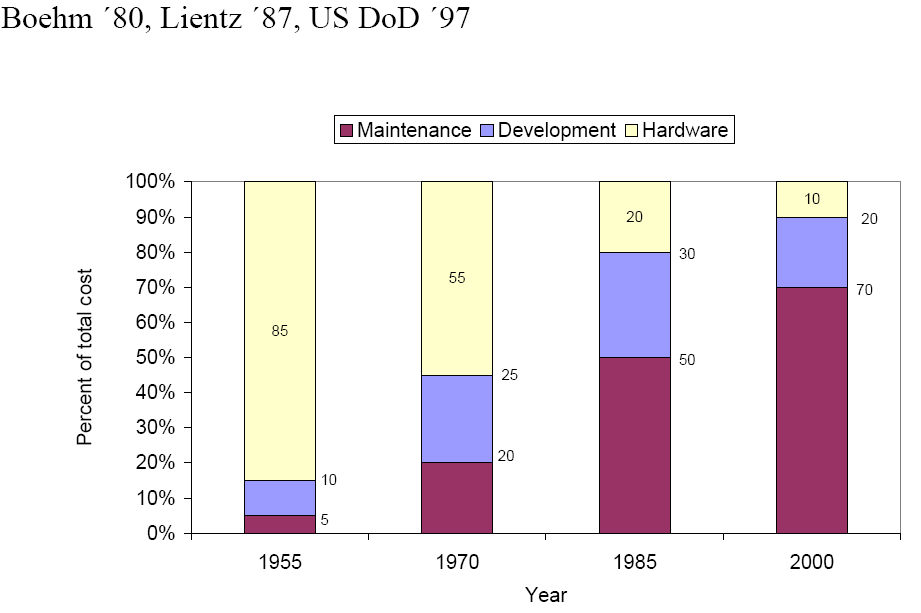
\includegraphics[width=\linewidth]{software-engineering/swMaintenanceCost}
%
\newpage
%\fi
\subsection{Standish Group Reports}
Based on more than 80000 software project there are the following comclusions:

%Anhand jährlicher Untersuchungen von mittlerweile über 80'000 kommerziellen
%Softwareprojekte werden die folgenden Schlussfolgerungen gezogen:

%(\href{http://www.standishgroup.com/sample_research/chaos_1994_1.php}
%  {www.standishgroup.com/sample\_research/chaos\_1994\_1.php}
%(\href{http://www.softwaremag.com/L.cfm?Doc=newsletter/2004-01-15/Standish}
%    {www.softwaremag.com/L.cfm?Doc=newsletter/2004-01-15/Standish})
\begin{center}
\begin{tabular}{lrr}
      & 1994 & 2004 \\
\hline
successful projects & 16 \% & 34 \%\\
 canceled software projects & 31 \% & 15 \% \\
cost of canceled software projects in Billion USD &  81  &  55\\
SW development cost in Billion USD &  250  &  255  \\
 average cost overrun & 180 \% & 43 \% \\
% Only 9\% of software projects for large companies were delivered
%  on time and within budget. For medium-sized and small companies, the
%  numbers improved to 16\% and 28\%, respectively.
\end{tabular}
\end{center}
\renewcommand{\arraystretch}{1.2}
\ifslides
{\footnotesize
\fi
\begin{tabular}[h]{lr|lr}
                  & \% OF &                        & \% OF \\
SUCCESSFUL PROJECTS & RESPONSES & CHALLENGED PROJECTS & RESPONSES \\
\hline
User involvement & 15.9 & Lack of user input & 12.8 \\
Executive mgmnt support & 13.9 & Incomplete requirements & 12.3 \\
Clear statement of requirements & 13.0 & Changing requirements & 11.8\\
Proper planning & 9.6 & Lack of executive support & 7.5 \\
Realistic expectations & 8.2 & Technology incompetence & 7.0 \\
Smaller project milestones & 7.7 & Lack of resources & 6.4 \\
Competent staff & 7.2 & Unrealistic expectations & 5.9 \\
Ownership & 5.3 & Unclear objectives & 5.3 \\
Clear vision and objectives & 2.9 & Unrealistic time frame & 4.3 \\
Hard-working, focused staff & 2.4 & New technology & 3.7 \\
Other & 13.9 & Other & 23.0 \\
\hline
\end{tabular}\\[2ex]
\ifslides
}
\fi
\begin{center}
\ifslides
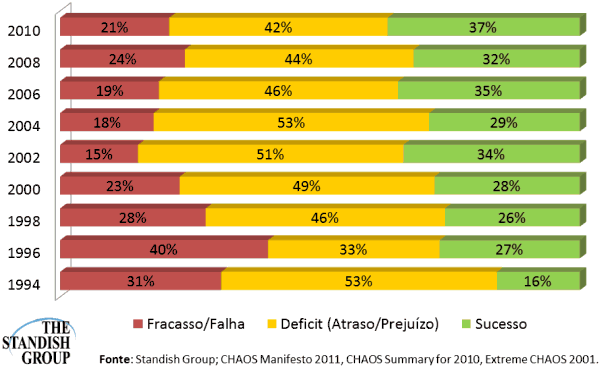
\includegraphics[width=0.9\linewidth]{software-engineering/standish_success_failure}
\else
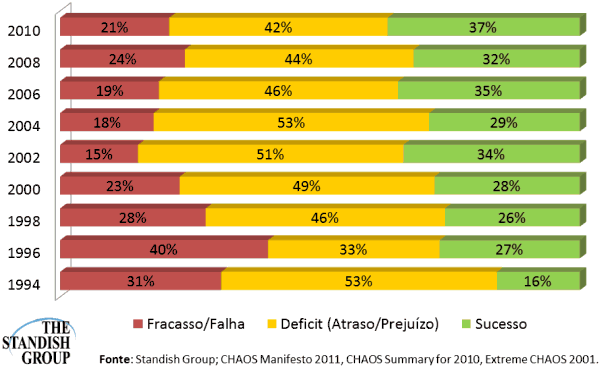
\includegraphics[width=0.6\linewidth]{software-engineering/standish_success_failure}
\fi
\end{center}
\ifslides
\newpage
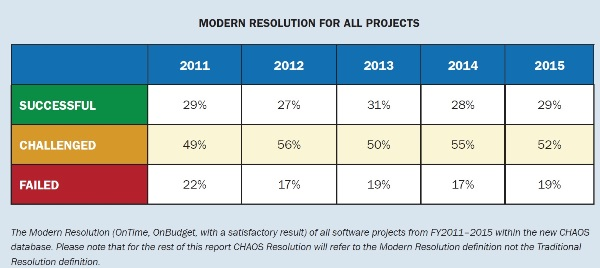
\includegraphics[width=\linewidth]{software-engineering/standish-1}
\newslide
\fi
  Research at the Standish Group also indicates that \hl{smaller time frames,
  with delivery of software components early and often, will increase the
  success rate}. Shorter time frames result in an iterative process
  of design, prototype, develop, test and deploy small elements. This
  process is known as growing software, as opposed to the old concept
  of developing software. Growing software engages the user earlier,
  each component has an owner or a small set of owners, and expectations
  are realistically set. In addition, each software component has a clear
  and precise statement and set of objectives. Software components
  and small projects tend to be less complex. Making the projects simpler
  as a worthwhile endeavor because complexity causes only confusion
  and increased cost.\\[2ex]
%-----------------------------------------------------------------------------
%\newpage
%\subsection{Definitionen}
%
\newpage
\section{Taking a Closer Look}
%\begin{description}
%\item[Systems-Engineering]
%Wegleitung, die auf bestimmten Denkmodellen und Grundprinzipien
%beruht, zur zweck\-m\"as\-si\-gen und zielgerichteten Gestaltung komplexer
%Systeme (W.F.Daenzer 1989).
%\item[Software] Die Programme, Verfahren, zugehörige Dokumentationen und
%  Daten, die mit dem Betrieb eines Computersystems zu tun haben (IEEE 610.12).
%\item[Software Engineering]
\structure{IEEE Standard Computer Dictionary} (Std 610):
\begin{quote}
(1) The application of a systematic, disciplined, quantifiable approach to the development,
   operation, and maintenance of software; that is, the application of engineering to software.

(2) The study of approaches as in (1)
\end{quote}
% Software Engineering Vocabulary:
%   https://pascal.computer.org/sev_display/index.action
%
% is the application of science and mathematics
%by which the capabilities of computer equipment
%are made useful to man via computer programs, procedures and associated
%documentation (B. Boehm 1981).
\newslide
\structure{Software Engineering Body of Knowledge} (SWEBOK V3):\\
%\href{https://www.computer.org/portal/web/swebok}{www.computer.org/portal/web/swebok}
\href{https://www.computer.org/education/bodies-of-knowledge/software-engineering}
  {www.computer.org/education/bodies-of-knowledge/software-engineering}
\ifslides

15 Knowledge Areas (KA) %Characterizing the Practice of Software Engineering:

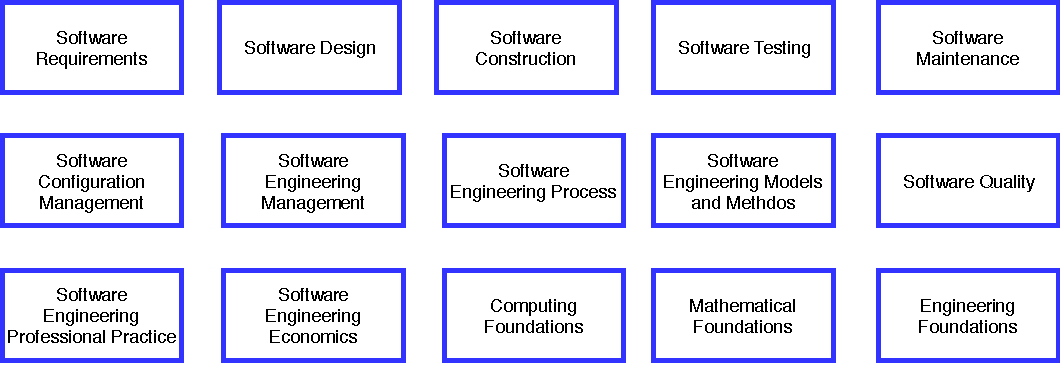
\includegraphics[width=\linewidth]{software-engineering/SWEBOK-KA}
\newslide
Covered in Modules Software Engineering% I / II:

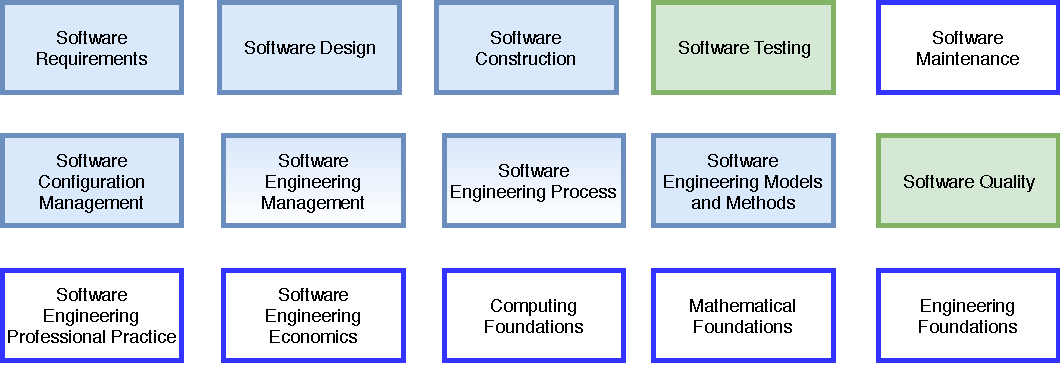
\includegraphics[width=\linewidth]{software-engineering/SWEBOK-KA2}
\newslide
\else
\begin{figure}[H]
  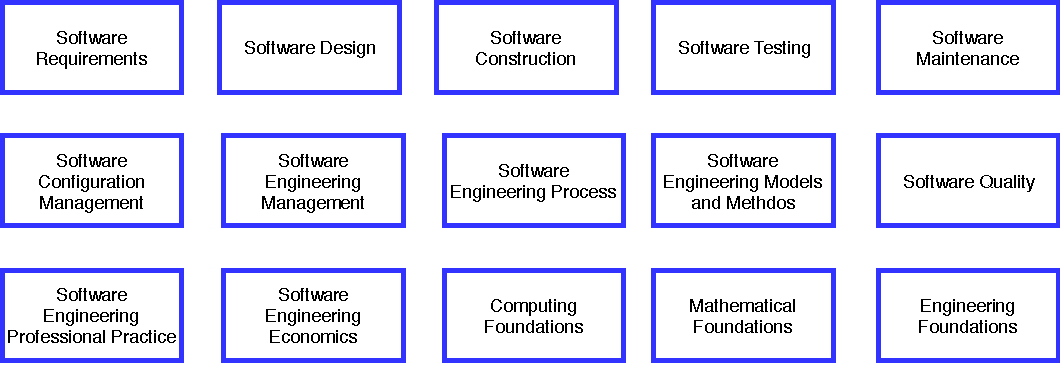
\includegraphics[width=\linewidth]{software-engineering/SWEBOK-KA}
  \caption{15 Knowledge Areas (KA)} %Characterizing the Practice of Software Engineering}
\end{figure}

\begin{minipage}{0.48\linewidth}
\fi
\begin{itemize}
\item \structure{Software Requirements}: elicitation, negotiation, analysis,
  specification, and validation,
  \item \structure{Software Design}: definition of the architecture, components, interfaces,
  \item \structure{Software construction}: detailed design, coding, unit testing,
    integration testing, debugging, verification and tools,
  \item \structure{Software Testing}: fundamentals of software testing; testing techniques;
    human-computer user interface testing and evaluation; test-related measures
  \item \structure{Software Maintenance}: program comprehension, re-engineering,
    reverse engineering, refactoring, software retirement; disaster recovery techniques, tools,
\newslide
\end{itemize}
\ifslides
\newslide
\else
\end{minipage}
\hfill
\begin{minipage}{0.48\linewidth}
\fi
\begin{itemize}
\item \structure{Software Configuration Management}: identification, control,
  status accounting, auditing; software release management and delivery, tools
\item \structure{Software Engineering Management}: process planning,
  estimation of effort, cost, and schedule, resource allocation, risk analysis,
  planning for quality;
  %software project enactment (measuring, reporting, and controlling; acquisition and supplier contract management);
  product acceptance; review and analysis of project performance; project closure; tools
\item \structure{Software Engineering Process}: software life cycle models,
  process assessment, tools
  \item \structure{Software Engineering Methods}: modeling, analysis %tools and methods
  \item \structure{Software quality}: verification, validation, reviews, audits, tools
\end{itemize}
\ifslides
\else
\end{minipage}
\hfill
\begin{minipage}[t]{0.48\linewidth}
\fi
\begin{itemize}
\item \structure{Software Engineering Professional Practice}:  standards,
  codes of ethics; group dynamics (working in teams, cognitive problem complexity,
  interacting with stakeholders, dealing with uncertainty and ambiguity,
  dealing with multicultural environments); communication skills
%\newslide
%\item Knowledge Areas Characterizing the Educational Requirements of Software Engineering
%  \begin{itemize}
\item \structure{Software Engineering Economics}: cost-benefit analysis,
  optimization, risk analysis, estimation, decision making
\end{itemize}
\ifslides
\else
\end{minipage}
\hfill
\begin{minipage}[t]{0.48\linewidth}
\fi
\begin{itemize}
\item \structure{Computing Foundations}: operation systems,
  networking, algorithms, parallel an distributed computing
\item \structure{Mathematical Foundations}: sets, relations, and
  functions; basic propositional and predicate logic;
  proof techniques; graphs and trees; discrete probability;
  grammars and finite state machines; and number theory.
\item \structure{Engineering Foundations}: statistical analysis;
  measurements and metrics; engineering design; simulation and modeling
\end{itemize}
\ifslides
\newslide
\else
\end{minipage}
\fi

\begin{minipage}{0.48\linewidth}
 7 Related Disciplines:
  \begin{itemize}
  \item Computer Engineering
  \item Computer Science
  \item General Management
  \item Mathematics
  \end{itemize}
\end{minipage}
\hfill
\begin{minipage}{0.48\linewidth}
  \begin{itemize}
  \item Project Management
  \item Quality Management
  \item Systems Engineering
  \end{itemize}
\end{minipage}
%\item[Projekt] ein zeitlich begrenztes, einmaliges Entwicklungsvorhaben zum
%L\"osen von Problemen innerhalb eines vorgegebenen Zielsystems. Es umfasst
%die Gesamtheit der f\"ur die Probleml\"osung notwendigen Entwicklungsarbeiten.
%\ifslides
%\newpage
%\fi
%\item[Projektmanagement] die Gesamtheit der organisatorischen und methodischen
%  Massnahmen zur ziel-, termin- und kostengerechten Abwicklung eines Projektes.
%
%  Dies umfasst (DIN 69 901):
%  \begin{itemize}
%    \item Führungsaufgaben: Zielsetzung,Zieleinhaltung, Entscheidung,
%    \item Führungsorganisation: Projektorganisation, Projektabwicklung,
%    \item Führungstechniken: Motivationstechnik, Besprechungstechnik,
%         Präsentationstechnik, Entscheidungsfindungstechnik
%    \item Führungsmitteln: Produkt- und Projektstrukturplanungssysteme,
%         Termin- / Kapazitäts-/ Kostenplanungs- und Steuerungssysteme
%       \end{itemize}
%
%
%\ifslides
%\newpage
%\fi
%   Die Ziele des Projektmanagements sind:
%\begin{itemize}
% \item Erstellen der erforderlichen Ergebnisse bzgl. Qualität und Funktion,
% \item     Reduzierung der Durchlaufzeit von Projekten,
%  \item     Reduzierung des Gesamtaufwands von Projekten,
%  \item     Erhöhung der Reaktionsfähigkeit der Projekte,
%  \item     Rechtzeitiges Erkennen und Vermindern von Risiken,
%  \item     Erhöhung der Transparenz über den Projektstand.
%  \end{itemize}
%\end{description}
\newpage
\subsection{Craft and Pragmatism}
Is software development more a \textcolor{blue}{\bfseries craft} than an \textcolor{OliveGreen}{\bfseries engineering} discipline?\\
(\href{http://www.developerdotstar.com/mag/articles/reeves_design.html}
{Jack W. Reeves, 1992})

Pragmatism considers words and thought as \hl{tools and instruments for prediction,
problem solving and action}, and rejects the idea that the function of thought is to
describe, represent, or mirror reality.

Pragmatists contend that most philosophical
topics—such as the nature of knowledge, language, concepts, meaning, belief, and
science—are all best viewed in terms of their \hl{practical uses and successes}.
%The philosophy of pragmatism ``emphasizes the practical application of ideas by acting on them to
%actually test them in human experiences''.
(\href{https://en.wikipedia.org/wiki/Pragmatism}{en.wikipedia.org/wiki/Pragmatism})

\newslide
{\bfseries Examples from The Pragmatic Programmer}\\
\href{https://blog.codinghorror.com/a-pragmatic-quick-reference}{blog.codinghorror.com/a-pragmatic-quick-reference}

%    Care About Your Craft
%    Why spend your life developing software unless you care about doing it well?
%
%    Think! About Your Work
%    Turn off the autopilot and take control. Constantly critique and appraise your work.
%
%    Provide Options, Don't Make Lame Excuses
%    Instead of excuses, provide options. Don't say it can't be done; explain what can be done.
\begin{itemize}
  \item \structure{Don't Gather Requirements – Dig for Them}
    Requirements rarely lie on the surface. They're buried deep beneath layers of assumptions, misconceptions, and politics.
  \item \structure{Work With a User to Think Like a User}
    It's the best way to gain insight into how the system will really be used.
  \item \structure{Program Close to the Problem Domain}
    Design and code in your user's language.
  \item \structure{Make Quality a Requirements Issue}
    Involve your users in determining the project's real quality requirements.
  \item \structure{There Are No Final Decisions}
    No decision is cast in stone. Instead, consider each as being written in the sand at the beach, and plan for change.
  \item \structure{Some Things Are Better Done than Described}
    Don't fall into the specification spiral – at some point you need to start coding.
  \item \structure{Don't Be a Slave to Formal Methods}
    Don't blindly adopt any technique without putting it into the context of your development practices and capabilities.
  \item \structure{Critically Analyze What You Read and Hear}
    Don't be swayed by vendors, media hype, or dogma. Analyze information in terms of you and your project.
%  \item
%    Costly Tools Don't Produce Better Designs\\
%    Beware of vendor hype, industry dogma, and the aura of the price tag. Judge tools on their merits.
  \item \structure{You Can't Write Perfect Software}
    Software can't be perfect. Protect your code and users from the inevitable errors.
\item \structure{Don't Live with Broken Windows}
    Fix bad designs, wrong decisions, and poor code when you see them.
%
%    Be a Catalyst for Change
%    You can't force change on people. Instead, show them how the future might be and help them participate in creating it.
%
%    Remember the Big Picture
%    Don't get so engrossed in the details that you forget to check what's happening around you.
%
%  \item
%    Invest Regularly in Your Knowledge Portfolio
%    Make learning a habit.
%  \item
%    It's Both What You Say and the Way You Say It
%    There's no point in having great ideas if you don't communicate them effectively.
  \item \structure{DRY – Don't Repeat Yourself}
    Every piece of knowledge must have a single, unambiguous, authoritative representation within a system.
%  \item
%    Make It Easy to Reuse
%    If it's easy to reuse, people will. Create an environment that supports reuse.
%
%    Eliminate Effects Between Unrelated Things
%    Design components that are self-contained. independent, and have a single, well-defined purpose.
%
%    Use Tracer Bullets to Find the Target
%    Tracer bullets let you home in on your target by trying things and seeing how close they land.
%
%  \item
%    Prototype to Learn
%    Prototyping is a learning experience. Its value lies not in the code you produce, but in the lessons you learn.
%  \item
%    Estimate to Avoid Surprises
%    Estimate before you start. You'll spot potential problems up front.
%  \item
%    Iterate the Schedule with the Code
%    Use experience you gain as you implement to refine the project time scales.
%
%    Keep Knowledge in Plain Text
%    Plain text won't become obsolete. It helps leverage your work and simplifies debugging and testing.
  \item \structure{Use the Power of Command Shells}
    Use the shell when graphical user interfaces don't cut it.
  \item \structure{Use a Single Editor Well}
    The editor should be an extension of your hand; make sure your editor is configurable, extensible, and programmable.
  \item \structure{Always Use Source Code Control}
    Source code control is a time machine for your work – you can go back.
%
%    Fix the Problem, Not the Blame
%    It doesn't really matter whether the bug is your fault or someone else's – it is still your problem, and it still needs to be fixed.
%
%    Don't Panic When Debugging
%    Take a deep breath and THINK! about what could be causing the bug.
%
%    "select" Isn't Broken.
%    It is rare to find a bug in the OS or the compiler, or even a third-party product or library. The bug is most likely in the application.
%
%    Don't Assume It – Prove It
%    Prove your assumptions in the actual environment – with real data and boundary conditions.
%
%    Learn a Text Manipulation Language.
%    You spend a large part of each day working with text. Why not have the computer do some of it for you?
%
%    Write Code That Writes Code
%    Code generators increase your productivity and help avoid duplication.
%
%    Design with Contracts
%    Use contracts to document and verify that code does no more and no less than it claims to do.

%    Crash Early
%    A dead program normally does a lot less damage than a crippled one.

%    Use Assertions to Prevent the Impossible
%    Assertions validate your assumptions. Use them to protect your code from an uncertain world.
%
%    Use Exceptions for Exceptional Problems
%    Exceptions can suffer from all the readability and maintainability problems of classic spaghetti code. Reserve exceptions for exceptional things.
%
%    Finish What You Start
%    Where possible, the routine or object that allocates a resource should be responsible for deallocating it.
  \item \structure{Minimize Coupling Between Modules}
    Avoid coupling by writing "shy" code and applying the Law of Demeter.
%
%    Configure, Don't Integrate
%    Implement technology choices for an application as configuration options, not through integration or engineering.
%
%    Put Abstractions in Code, Details in Metadata
%    Program for the general case, and put the specifics outside the compiled code base.
%
%    Analyze Workflow to Improve Concurrency
%    Exploit concurrency in your user's workflow.

%    Design Using Services
%    Design in terms of services – independent, concurrent objects behind well-defined, consistent interfaces.

%    Always Design for Concurrency
%    Allow for concurrency, and you'll design cleaner interfaces with fewer assumptions.
%  \item
%    Separate Views from Models\\
%    Gain flexibility at low cost by designing your application in terms of models and views.
%
%    Use Blackboards to Coordinate Workflow
%    Use blackboards to coordinate disparate facts and agents, while maintaining independence and isolation among participants.

%    Don't Program by Coincidence
%    Rely only on reliable things. Beware of accidental complexity, and don't confuse a happy coincidence with a purposeful plan.

%    Estimate the Order of Your Algorithms
%    Get a feel for how long things are likely to take before you write code.

%    Test Your Estimates
%    Mathematical analysis of algorithms doesn't tell you everything. Try timing your code in its target environment.
  \item \structure{Refactor Early, Refactor Often}
    Just as you might weed and rearrange a garden, rewrite, rework, and re-architect code when it needs it. Fix the root of the problem.
    \newslide
  \item \structure{Design to Test}
    Start thinking about testing before you write a line of code.
  \item \structure{Test Early. Test Often. Test Automatically}
    Tests that run with every build are much more effective than test plans that sit on a shelf.
%  \item
%    Test Your Software, or Your Users Will
%    Test ruthlessly. Don't make your users find bugs for you.
%
%    Don't Use Wizard Code You Don't Understand
%    Wizards can generate reams of code. Make sure you understand all of it before you incorporate it into your project.
%  \item
%    Abstractions Live Longer than Details\\
%    Invest in the abstraction, not the implementation. Abstractions can survive the barrage of changes from different implementations and new technologies.
%  \item
%    Use a Project Glossary
%    Create and maintain a single source of all the specific terms and vocabulary for a project.

%    Don't Think Outside the Box – Find the Box
%    When faced with an impossible problem, identify the real constraints. Ask yourself: "Does it have to be done this way? Does it have to be done at all?"

%    Start When You're Ready.
%    You've been building experience all your life. Don't ignore niggling doubts.
%  \item
%    Organize Teams Around Functionality
%    Don't separate designers from coders, testers from data modelers. Build teams the way you build code.
  \item \structure{Don't Use Manual Procedures}
    A shell script or batch file will execute the same instructions, in the same order, time after time.

%    Coding Ain't Done 'Til All the Tests Run
%    'Nuff said.

%    Use Saboteurs to Test Your Testing
%    Introduce bugs on purpose in a separate copy of the source to verify that testing will catch them.

%    Test State Coverage, Not Code Coverage
%    Identify and test significant program states. Just testing lines of code isn't enough.

%    Find Bugs Once
%    Once a human tester finds a bug, it should be the last time a human tester finds that bug. Automatic tests should check for it from then on.

%    English is Just a Programming Language
%    Write documents as you would write code: honor the DRY principle, use metadata, MVC, automatic generation, and so on.

%    Build Documentation In, Don't Bolt It On
%    Documentation created separately from code is less likely to be correct and up to date.

%    Gently Exceed Your Users' Expectations
%    Come to understand your users' expectations, then deliver just that little bit more.
  \item \structure{Sign Your Work}
    Craftsmen of an earlier age were proud to sign their work. You should be, too.
\end{itemize}
%
\subsection{A Simplified Model}
%\vfill
\begin{minipage}[t]{0.45\linewidth}
\textcolor{blue}{\large\bfseries Software Development}
\begin{description}
  \item[Requirements]: elicitation, negotiation, analysis, specification, and validation,
  \item[Design]: architecture, components, interfaces,
  \item[Construction]: coding, unit \& integration testing, documentation %integration testing, debugging,
\end{description}
\end{minipage}
\hfill
\begin{minipage}[t]{0.45\linewidth}
\textcolor{OliveGreen}{\large\bfseries Project Management:}
\begin{description}
\item[Configuration Management]: change control, release management
\item[Process Life Cycle]: planning, resource allocation, risk analysis
\item[Quality Management]: verification, validation, reviews
\end{description}
\end{minipage}

\section{Sample Software Projects}
\subsection{Ariane 5}
On June 4, 1996 an unmanned Ariane 5 rocket launched by the European Space
Agency exploded just forty seconds after its lift-off from Kourou, French
Guiana. The rocket was on its first voyage, after a decade of development
costing \verb|$|7 billion. The destroyed rocket and its cargo were valued at
\verb|$|500 million. A board of inquiry investigated the causes of the
explosion and in two weeks issued a report. It turned out that the cause
of the failure was a software error in the inertial reference system (IRS)
untested for use in a new launch environment.
Specifically a 64 bit floating point number relating to the horizontal
velocity of the rocket with respect to the platform was converted to a 16 bit
signed integer. The number was larger than 32767, the largest integer
storeable in a 16 bit signed integer, and thus the conversion failed.\\
(\href{http://www-users.math.umn.edu/~arnold/disasters/ariane.html}
{http://www-users.math.umn.edu/~arnold/disasters/ariane.html})

\section{Software Engineering in industrial automation management}
Software in the field of industrial automation include the
following:
\begin{itemize}
\item Condition monitoring for large machines
\item Measurement and control
\item Safety and security management
\end{itemize}

%TODO

\section{Software Engineering in health care and biomedicine}
Software in health care is incredibly diverse. There are
many different working environments:
\begin{itemize}
\item Creating and managing software systems that connect researchers with
clinical experiment data (e.g. clinical trial)
\item Developing mobile application to monitor and collect data of
patients (e.g. collecting data with a smart watch).
\item Providing health care providers with data records about a
patient (e.g. doctor appointment).
\item Implement software systems which allows the handling of big data sets (
e.g. creating new software to predict skin cancer based on historical data).
\item Implement software systems for embedded devices (
e.g. software for a ventilator)
).
\item Implement software systems to support any health care environment (
e.g. electronic lab journal).
\item ... and many more
\end{itemize}

There are several aspects which must be considered:

\begin{itemize}
\item Data Security: handling of patient data
\item Reliability: devices are responsible for the health of patients
(e.g. a ventilator)
\item Traceability: Each change in a system must be documented
(e.g. which input data and source code was used to create the output data)
\end{itemize}

\section{Exercises}
\begin{enumerate}
\item What are the basic tasks that all software engineering projects must handle?
\item List five tasks that might be part of software deployment and explain why.
\item Collect several reasons why software engineering projects could fail.
\end{enumerate}

%

%\newpage
% -----------------------------------------------------------------------
\chapter{Course project}
%-----------------------------------------------------------------------
\section{Raspberry Pi}
Raspberry Pi is a series of small single-board computers developed in the
United Kingdom by the Raspberry Pi Foundation in association with Broadcom.
Early on, the Raspberry Pi project leaned towards the promotion of teaching
basic computer science in schools and in developing countries.
Later, the original model became far more popular than anticipated,
selling outside its target market for uses such as robotics. It is now
widely used in many areas, such as for weather monitoring,
because of its low cost and high portability.

\begin{centering}
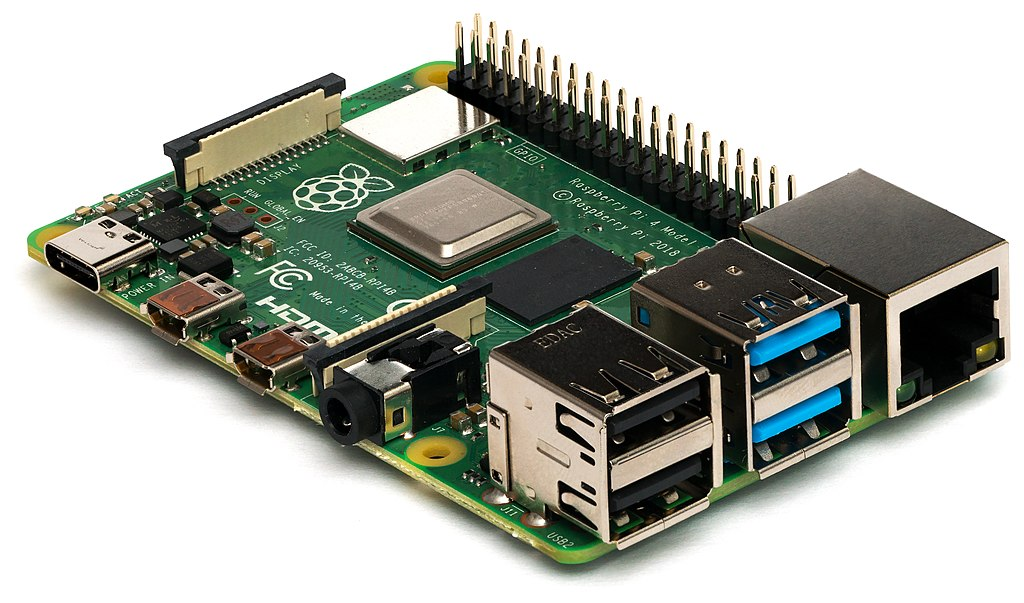
\includegraphics[width=300pt]{images/coursework/raspberrypi.jpeg}\\
(Source: https://www.wikipedia.org)
\end{centering}

\subsection{GPIO}
A powerful feature of the Raspberry Pi is the row of GPIO
(general-purpose input/output) pins along the top edge of the board.
A 40-pin GPIO header is found on all current Raspberry Pi boards.
Any of the GPIO pins can be designated (in software) as an input or output
pin and used for a wide range of purposes.

\begin{centering}
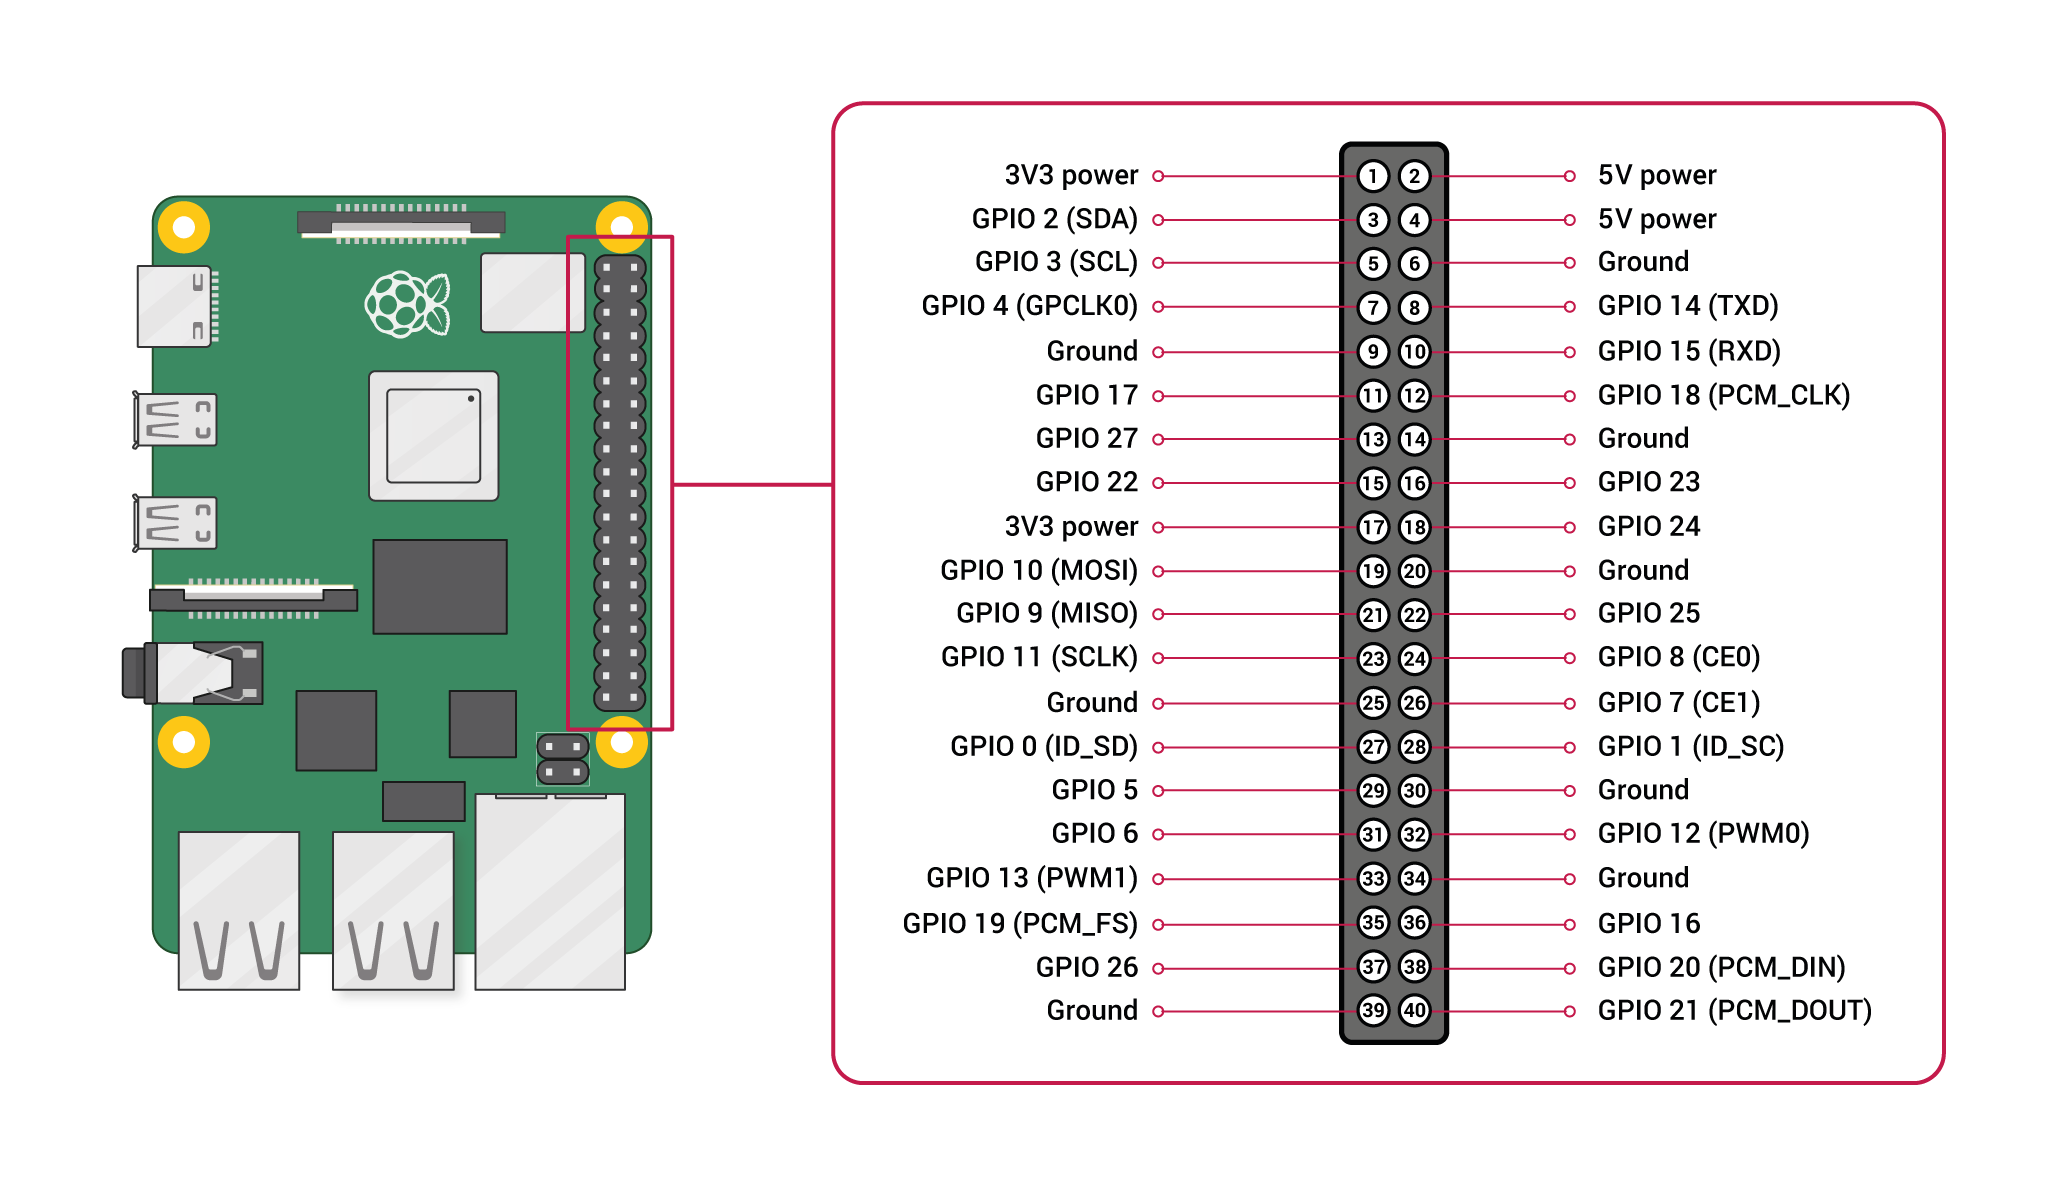
\includegraphics[width=360pt]{images/coursework/gpio.png}\\
(Source: https://www.raspberrypi.org)
\end{centering}

\section{Software}
This software project will develop a web application which could
be used to control external devices which are connected to the
GPIO system of a Raspberry Pi.

%%\newpage
% -----------------------------------------------------------------------
\chapter{Coursework}
%-----------------------------------------------------------------------
\section{Introduction}
A project will cover most of the topics from this course. At the end
of each chapter, there will be a set of exercises which are used to
strengthen the knowledge in software engineering. In addition, each
student will have the possibility to play around with the tools
demonstrated in this course.\\
For all the coursework, each student needs to have a computer
(Windows, OSX or Linux) with the possibility to install additional
software.

\subsection{Projects}
There are two projects available. The two projects are
developed for the following two courses:

\begin{itemize}
\item Gene Information Service (FHNW - Master Medical Informatics)
\item Raspberry Pi GPIO Web Application (FHNW - Master Automation Management)
\end{itemize}


\section{Gene Information Service}
The gene information service will be a system with three components:

\begin{itemize}
\item Data Loader\\
This component loads a data file from NCBI into a database
\item Gene Information Service\\
This component will provide a REST based service which could
be used by other applications to retrieve gene specific information
\item Gene Search Web Application
This component will provide a simple Java based Web Application
which utilizes the Gene Information Service
\end{itemize}

\section{What is a gene}
In biology, a gene is a sequence of nucleotides in DNA or RNA that encodes the
synthesis of a gene product, either RNA or protein.\\
(Source: Gene: Wikipedia)

\begin{centering}
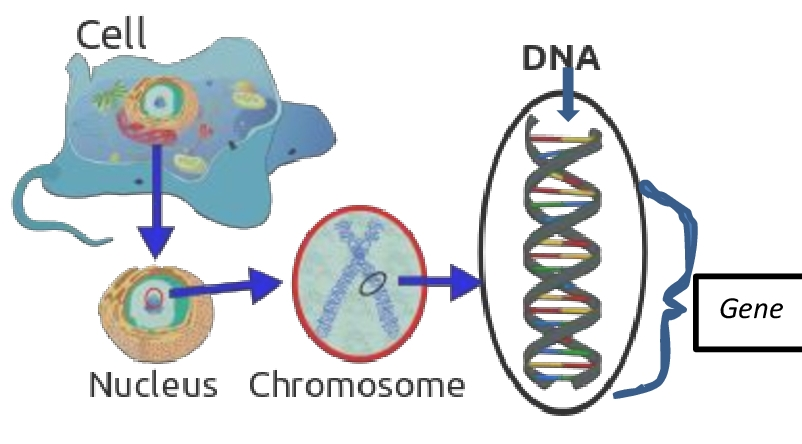
\includegraphics[width=250pt]{images/coursework/geneinfo.jpg}\\
\end{centering}

\section{Basic Idea}
The gene information service will provide a system to retrieve
information for a given gene.
\begin{itemize}
\item The data which is used is coming from NCBI. The raw data size
is in the area of 4GB.
\item This data will be loaded into a database (e.g. MySQL, Postgres).
This will be done by the first component, \emph{Data Loader}
\item The data will be available over a REST interface. This is
the second component. The service will be connected to the database
a will provide query functionalities for end users.
\item A end user application will be created, where potential
users could create queries and display the gene information data.
This could be a web application or also a mobile application. In this
project, we will use a web application.
\end{itemize}

\section{Exercises}
\begin{enumerate}
\item In each project it is important to understand the data which
is used. Download the gene information file from the NCBI ftp server:\\
\vspace{3mm}
\verb|ftp://ftp.ncbi.nlm.nih.gov/gene/DATA/gene_info.gz|\\
\vspace{3mm}
Try to answer the following questions:
\begin{itemize}
\item How many genes does the file contain?
\item What kind of information is in the \verb|tax_id| field?
\item Which gene types do exist?
\item Which gene type is the one which appears the most?
\end{itemize}

\end{enumerate}

%
% TODO: Scrum
% Joel Spolsky
% https://www.joelonsoftware.com/2007/10/26/evidence-based-scheduling/
%
\newpage
%-------------------------------------------------------------------------
\chapter{Project Planning}
%
This chapter will cover methods how to control a project. Stakeholders
measure projects by how well they are executed within the project
constraints or baselines. A project baseline is an approved plan for a
portion of a project. It is used to compare actual performance to
planned performance and to determine if project performance is within
acceptable guidelines.\\
The following 4 project baselines should be considered:
\begin{itemize}
\item Quality
\item Schedule
\item Scope
\item Budget
\end{itemize}

Results:
\begin{itemize}
\item {\textbf Cost plan}: Creating budget / offer. %Ausarbeitung des Budgets resp. der Offerte
\item {\textbf Time plan}: Define activities, deadlines and milestones. %Festlegung der Aktivitäten, Termine und Meilensteine
\item {\textbf Employee plan}: Nomination of people and their working time. %Benennung der beteiligten Mitarbeiter/innen mit ihren Einsatzzeiten
\item {\textbf Organization plan}: Agreement of team structure, nomination of responsible persons. %Festlegung der Team-Struktur, Bezeichnung der Verantwortlichkeiten
\item {\textbf Quality plan}: Compilation of documents, tools and methods to ensure quality. %Zusammenstellung der Dokumente, Werkzeuge und Methoden zur Sicherstellung der Qualit\"at
\item {\textbf Project monitor plan}: Agreement of actions to control the project and if needed how to change the plans. %Festlegung der Massnahmen zur Kontrolle der Planeinhaltung, ggf. zur \"Anderung der Pl\"ane
\item {\textbf Configuration management plan}: Agreement of actions to control changes in documents, code or data (or any other resources). %Festlegung der Massnahmen zur Kontrolle der \"Anderungen in den Dokumenten, Programmen und Daten
\item {\textbf Education plan}: Definition of education for internal (project team) and external people (users, operating stuff). %Festlegung der internen (Mitarbeiter) und externen (Kunde, Anwender, Systembetreiber) projektspezifischen Ausbildung
\item {\textbf Risk management plan}: Agreement of actions to avoid or mitigate risks. %Festlegung der Massnahmen zur Vermeidung eines eventuellen Disasters.
\end{itemize}
\newpage
%--------------------------------------------------------------------------
\section{Classical/Traditional project planning}
\ifslides
\begin{center}
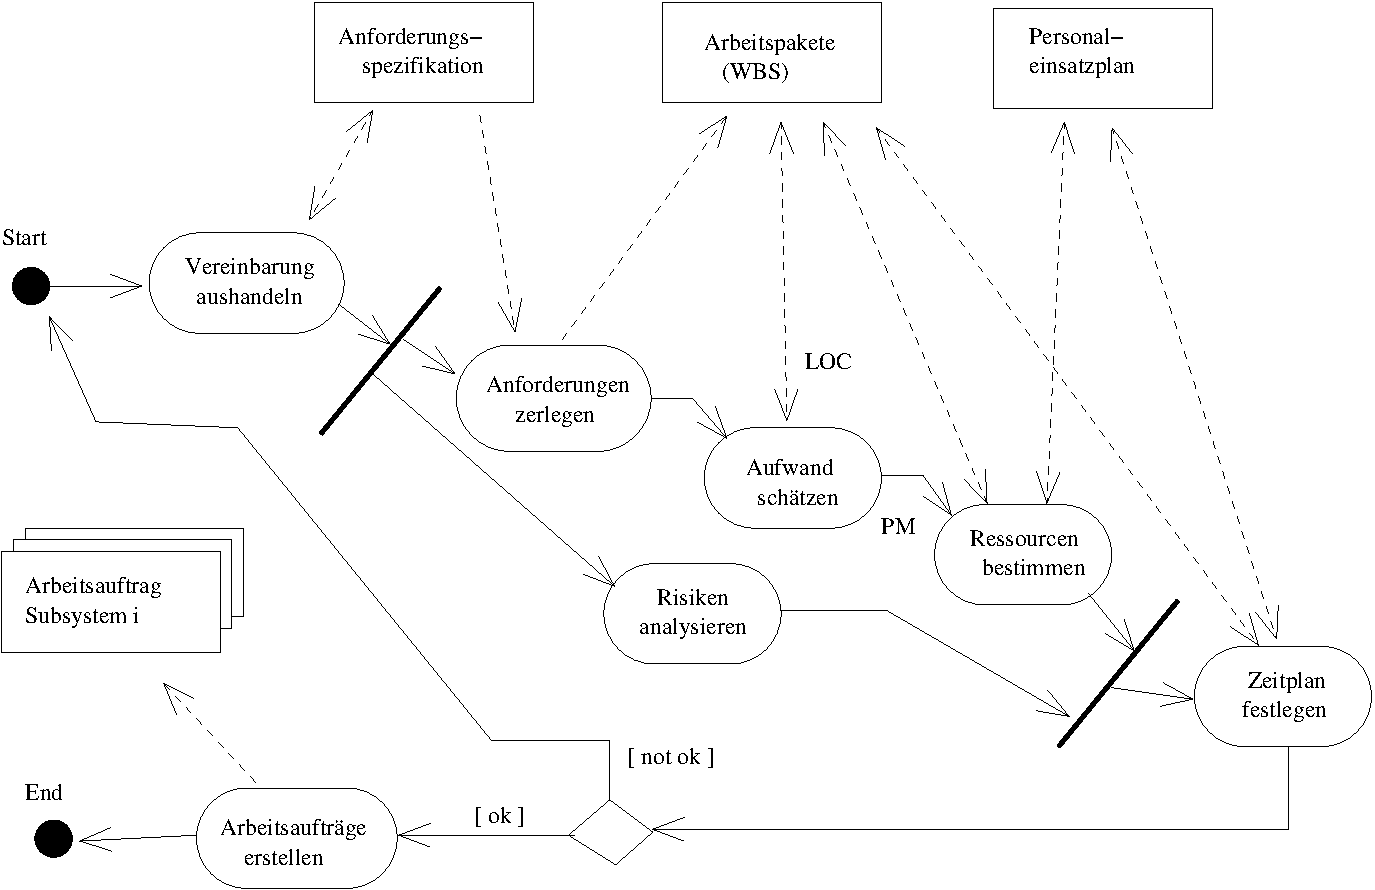
\includegraphics[width=0.85\linewidth]{lifecycle/xfig/planung}
\end{center}
\else
The process to create a project plan contains the following
activities:\\[3ex]
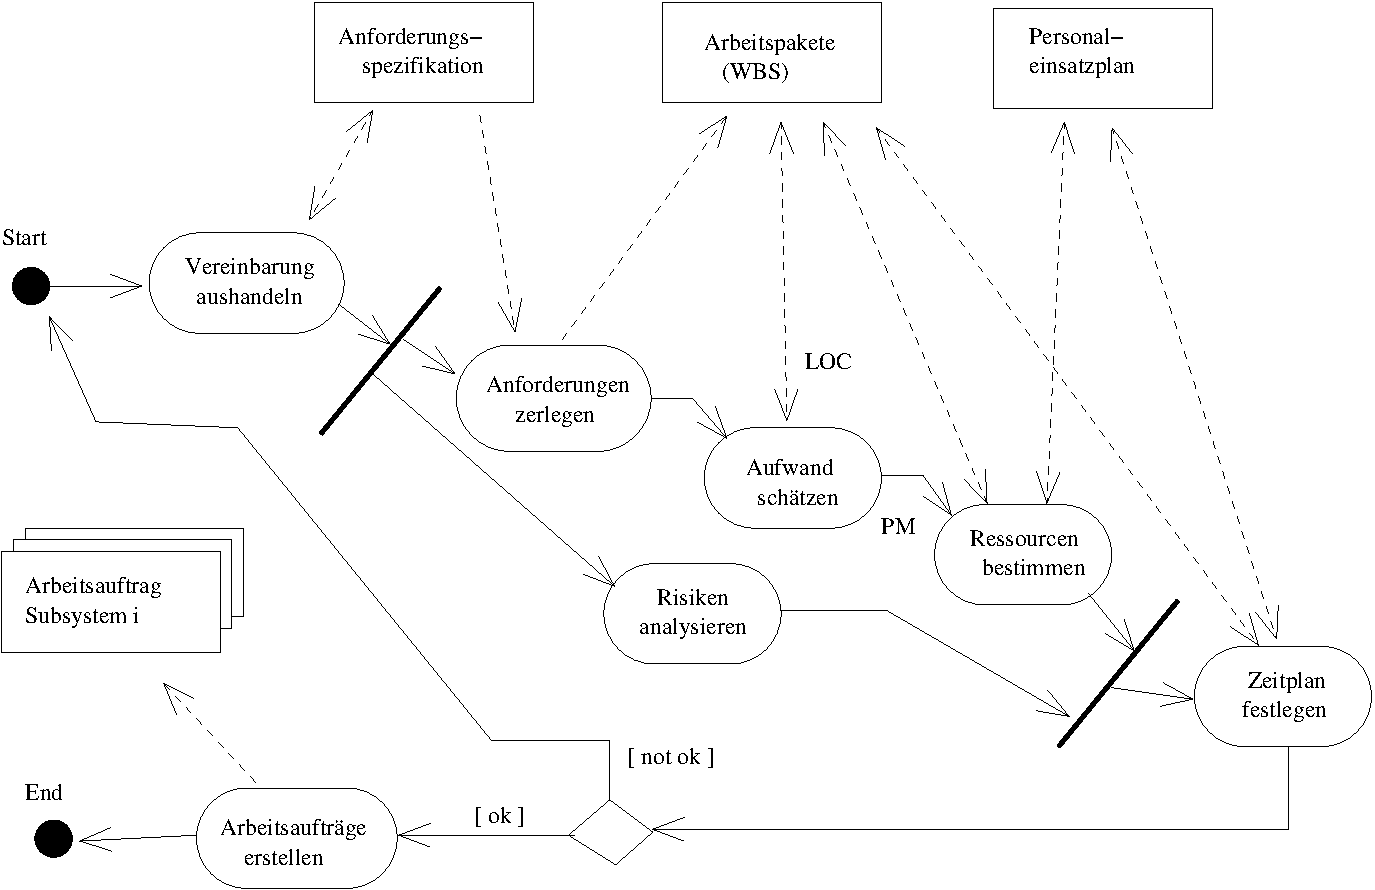
\includegraphics[width=\linewidth]{lifecycle/xfig/planung}\\[2ex]
\fi
\begin{enumerate}
\item \structure{Arrange agreement}:
  Define the project scope with a high level time schedule,
  point in time of devliverables, definition of mile stones.
  %Festlegung des Projektumfanges mit
  %einer groben Terminplanung, Abgabezeitpunkte der Liefergegenstände,
  %(engl. deliverables), Definition der Meilensteine
\item \structure{Breakdown requirements}:
  Breakdown the requirements into work packages according to the defined
  deliverables, create WBS (work breakdown structure). Recommended time
  for one work package is 4-6 weeks.
  %an den Liefergegenständen orientierte Zerlegung
  %in ``handhabbare'' Arbeitspakete, Aufstellung des Projektstrukturplans
  %(engl. Work breakdown structure WBS), empfehlenswerte Grössenordnung: 4-6
  %Wochen Zeitdauer pro Arbeitspaket,
\item \structure{Estimate effort}:
  Estimate effort for each package based on a value which could be measured.
  For software components, this could be LOC (lines of code). The LOC value
  could be used to get the amount of time needed for that component.
  %am besten auf Basis einer
  %(messbaren) Grössenschätzung für einzelne Arbeitspakete, bei SW-Komponenten
  %z.B: Lines of Code (LOC), daraus kann mittels
  %Erfahrungswerten der Aufwand in Personenmonaten (PM) bestimmt
  %werden,
\newslide
\item \structure{Define resources}:
  Assign people to activities with respect of their
  availability, qualification (education) and demand.
  The best way to do that is the usage of a model with
  roles and responsibilities.
  %Zuordnung der Personen zu den Aktivitäten
  %entsprechend des Bedarfes, ihrer Qualifikationen und Verfügbarkeit,
  %idealerweise auf Basis von Rollen und Verantwortlichkeiten
\item \structure{Analyse risks}:
  Identify and prioritize potential risks and possible actions.
  %Identifikation/Priorisierung der potentiellen
  %Probleme und möglicher Gegenmassnahmen
\item \structure{Define schedule}:
  Description of all work packages and their time dependencies.
  When is the final point in time to deliver a package, are there any
  dependencies to other packages? This is typically done with a
  gantt chart or network diagram.
  %Beschreibung/Darstellung der terminlichen
  %Rahmenbedingungen der
  %Aktivitäten sowie ihrer gegenseitige Abhängigkeiten (z.B. durch
  %Tabellen, Netzplantechnik, Ganttdiagramme) unter Berücksichtigung der Risiken
\end{enumerate}
\newpage
%-------------------------------------------------------------------
\section{Agile project planning}
Software development is a constant dialog between \emph{What is possible} and
\emph{What is needed}.
%
\begin{itemize}
\item \structure{Planning}: only plan for the next
  iteration, version. Not more!
\item \structure{Responsibility} will be taken over, not assigned
\item \structure{Estimates}: the responsible persons define the effort and duration
\item \structure{Priorities} define the order,
\end{itemize}

\newslide
The business side (Product Owner) decides
\begin{itemize}
\item \structure{MVP}: Minimal viable product. How should the problem be solved to
bring additional value. What is to much, what is not enough?
\item \structure{Priority}: Which tasks should be executed first?
\item \structure{Release}: Which pieces should be part in the next release?
\item \structure{Delivery}: Which timeframe is available to be successful?
\end{itemize}

\newslide
The developers have the freedom to take over responsibility and decide for
\begin{itemize}
\item \structure{Effort}: how long will it take to implement a specific feature?
\item \structure{Consequences}: what are the consequences for a taken approach?
\item \structure{Process}: what is the structure for the work and the team?
\item \structure{Planning}: when will the features be delivered
\end{itemize}

%
\newpage
\subsection{Cost Estimation}
The total costs of software projects contains
%Die Totalkosten einer Software-Entwicklung setzen sich zusammen aus:
\begin{itemize}
\item {\textbf Software-Cost}: software, licenses
\item {\textbf Hardware-Cost}: infrastructure (own hardware, cloud-based systems)
\item {\textbf Personal-Cost}: Salary, Expenses
\end{itemize}
\ifslides
\newpage
\fi
Precision of the cost estimation:
\ifslides
\begin{center}
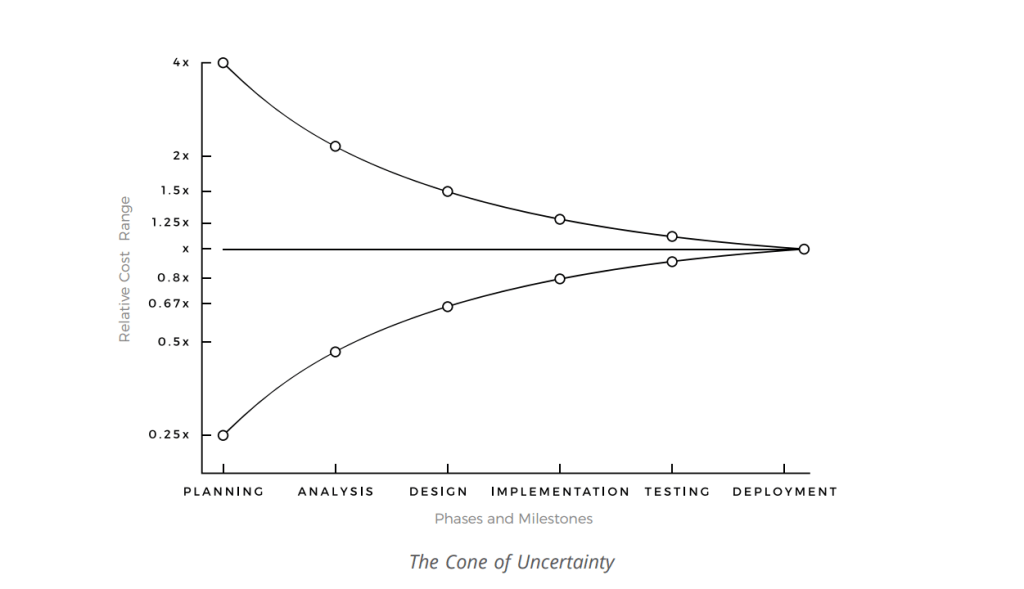
\includegraphics[width=0.75\linewidth]{lifecycle/img/cost_estimates}\\[2ex]
\end{center}
\else
\\[2ex]
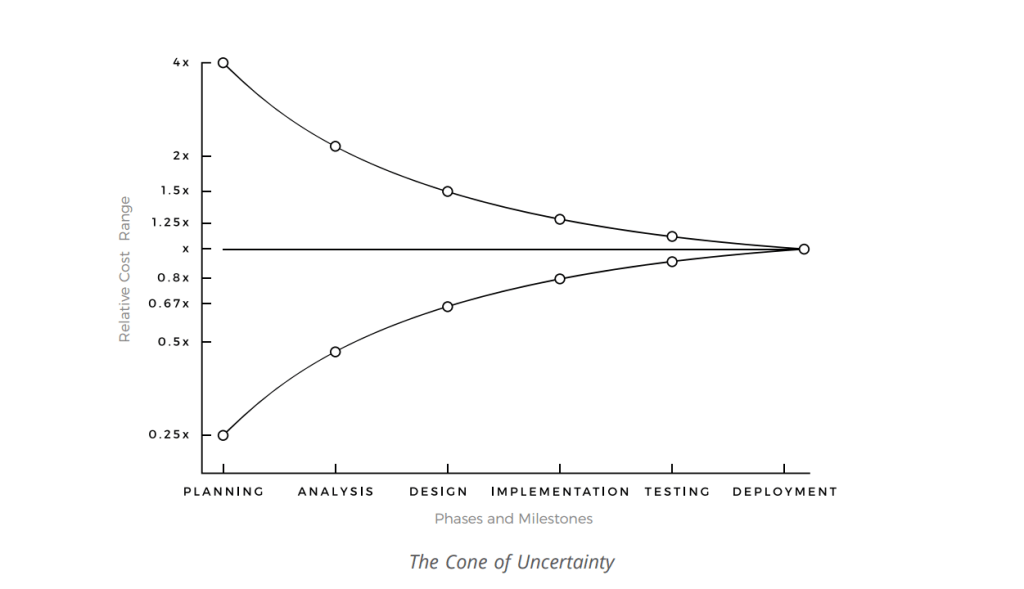
\includegraphics[width=1.0\linewidth]{lifecycle/img/cost_estimates}\\[2ex]
\fi
%
Influencing factors to estimate the costs:
\begin{itemize}
\item {\textbf Size}: Lines of code, classes, methods
\item {\textbf Complexity}: Dependency between the modules, is it possible to build modules?, HW/SW environment
\item {\textbf Experience}: Number of similar executed projects
\item {\textbf Reliability}: error rate, system stability
\end{itemize}
\newpage
There are several methods to estimate the costs:
\begin{itemize}
\item Empiric estimation methods:
\begin{itemize}
\item {\bfseries Expert judgment:}
  Several experts on the proposed software development techniques and
  the application domain are consulted. They each estimate the project
  cost. These estimates are compared and discussed. The estimation
  process iterates until an agreed estimate is reached.
  %Vergleich mit durchgeführten Projekten mittels
  %direkter Analogieschätzung, Schätzung durch Zerlegung in Teilaufgaben,
  %Drei-Punkt-Schätzung (optimistisch, realistisch, pessimistisch),
\item {\bfseries Delphi method:}
  Delphi technique is quite an old but efficient forecasting method.
  It follows an interactive approach which relies on exchange of ideas.
  The team is composed of a group of experts in their respective domains,
  who answers the queries in two or more rounds. Every time a facilitator
  provides a summary of the collected ideas, which is revised by the
  experts if required. The process of opinion and revaluation goes on
  until a final consensus is reached.\\
  Delphi technique relies its assumption on the fact that assimilation
  of ideas from a structured group leads to a productive outcome.
  %mehrere Experten geben unabhängig voneinander
  %eine Schätzung ab, anschliessend wird der Mittelwert bekannt gegeben und das
  %Verfahren solange wiederholt, bis alle Schätzungen einigermassen bei
  %einander liegen,
\end{itemize}
\ifslides
\newpage
\fi
\item Algoritmic estimation methods:
\begin{itemize}
\item {\bfseries Function Point Analysis:}
  Function Point Analysis is a standardized method used commonly as
  an estimation technique in software engineering.\\
  In simple words, FPA is a technique used to measure software
  requirements based on the different functions that the requirement
  can be split into. Each function is assigned with some points based
  on the FPA rules and then these points are summarized using
  the FPA formula. The final figure shows the total man-hours
  required to achieve the complete requirement.
  %Zählung und Gewichtung der Funktionen unter
  %Berücksichtigung
  %der Schnittstellen, Eingaben, Ausgaben, Umformungen, Abfragen und
  %Datenbestände,
  %nicht geeignet für Programme mit hoher algorithmischer Komplexität und/oder
  %komplexer Benutzerschnittstelle, kaum messbar
\item {\bfseries Widget Point Analysis:}
  Count the UI (user interface) elements and calculate out of this
  number the function points. Only useful for software with user interfaces and
  not many algorithmic calculations in the background.
  %Zählung der User-Interface-Elemente und daraus
  %Ermittlung
  %der Funktionspunkte, nur für GUI-Programme mit geringer algorithmischer
  %Komplexität geeignet, leichte Reproduzier- und Messbarkeit
\item {\bfseries Lines of Code (LOC):}
  Easy measurement method. Dependent on the programming language and the
  available libraries.
  %einfache Messbarkeit jedoch abhängig von der
  %Programmiersprache
  %und der verwendeten Bibliotheken (libraries), kann im Verlauf eines
  %Projektes stark schwanken
\end{itemize}
\ifslides
\newpage
\fi
\item Other methods:
  \begin{itemize}
  \item {\bfseries Pricing to win }:
  The software cost is estimated to be whatever the customer has
  available to spend on the project. The estimated effort depends on the
  customer's budget and not on the software functionality.
  \item {\bfseries Pain threshold method}:
  Highest price which the customer is willing to pay
  %Soviel, wie der Auftraggeber gerade noch
  %bereit ist zu zahlen.
\item {\bfseries Parkinson's Law}:
Parkinson's Law states that work expands to fill the time available. The
cost is determined by available resources rather than by objective
assessment. If the software has to be delivered in 12 months and 5
people are available, the effort required is estimated to be 60 personmonths.
  \end{itemize}
\end{itemize}
\ifslides
\newpage
\fi
\underline{Function point analysis} (A.J. Albrecht)
Function points are used to compute a functional size measurement
(FSM) of software.: (\href{http://www.ifpug.org}{www.ifpug.org})
%Weitere Informationen: International Function Point User Group
\begin{center}
\begin{tabular}{|l|l|l|l|}
\hline
Category & Number & Value (low) average (high) & Total \\
\hline
External inputs & &  x (3) 4 (6) & \\
External outputs & & x (4) 5 (7) & \\
External inquiries & & x (3) 4 (6) & \\
Internal logical files & & x (7) 10 (15) & \\
External interface files & & x (5) 7 (10) & \\
\hline
\multicolumn{3}{|l|}{Total}  &\\
\hline
\end{tabular}
\end{center}
In a second step, the calculated function points could be converted into
LOC (lines of code):
%Ein Nachteil dieses Verfahrens ist, dass Function-Points nicht
%gemessen werden können. Albrecht schlägt deshalb vor, aus dem erhaltenen Wert
%in einem zweiten Schritt die Anzahl der
%Programmzeilen zu bestimmen.
\begin{center}
\begin{tabular}{|l|c|}
\hline
Programming language & LOC per FP \\
\hline
Assembler & 320 \\
C         & 128 \\
Fortran   & 128 \\
Pascal    & 91 \\
%Modula 2  & 80 \\
C++/Java  & 53 \\
SQL       & 13 \\
\hline
\end{tabular}
\end{center}
Attention: this method does not reflect the re-usage of software
components!
%Achtung:  bei dieser Methode wird die Wiederverwendung von
%Softwarekomponenten nicht berücksichtigt.

\vspace{5mm}

\newslide
%-------------------------------------------------------------------------------
%\subsection*{Kostensch\"atzung}
\underline{Widget point analysis} (H. Krasemann)\\[2ex]
Calculate the number of function points based on the elements of the
user interface.
%Aus der Anzahl der Elemente der Benutzeroberfläche die Funktionspunkte bestimmen:
\begin{equation}
 function points = 2\cdot widget points
\end{equation}
\begin{itemize}
\item {\bfseries Input widgets:} Textfield, Combobox, Menubutton, Radiobutton, Pushbutton,
  Checkbox
\item {\bfseries Describing widgets:} Label, Separator, Group box, Window
\item {\bfseries Composite widgets:} Notebook, Table, Scrollbar, List
\item {\bfseries Menu widgets:} Menu bars, Men items
\end{itemize}

\newslide
Example:%\\[3ex]

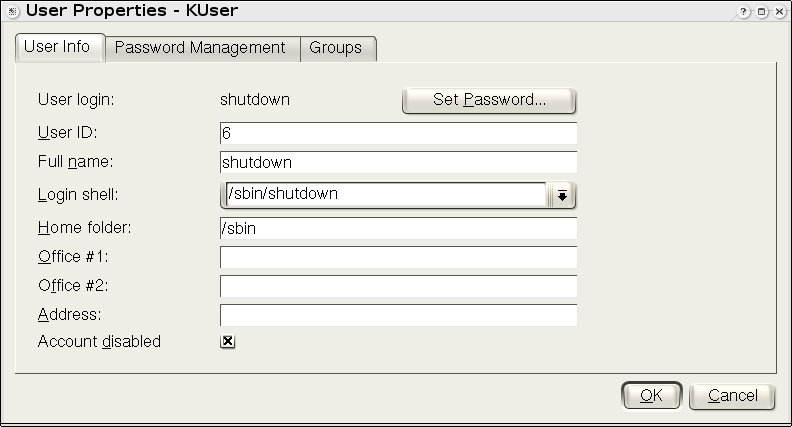
\includegraphics[width=\linewidth]{lifecycle/img/kuser}
%Beispiel:\\[2ex]
%\begin{tabular}{lr}
%Eingabewidgets & 9\\
%Beschreibende Widgets & 17 \\
%Zusammengesetzte Widgets & 1 \\
%\hline
%TOTAL  Widgetpunkte           & 27 \\
%TOTAL  Funktionspunkte           & 54 \\
%TOTAL LOC (C++)            & 2862 \\
%\end{tabular}
\newpage
%-------------------------------------------------------------------
%\section*{Projektplanung}
%\subsection*{Kostensch\"atzung}
\underline{COCOMO} (COnstructive-COst-MOdel, B. Boehm)
\begin{enumerate}
\item Calculation of the effort in person month:
\begin{equation}
 E_i = a \cdot KDL^b
\end{equation}
with the factor $a$\, the exponent $b$\
and $KDL$ as number of delivered lines of code (in thousand)
(Kilo-delivered-lines).\vspace{0.8cm}\\
\begin{tabular}{|l|cc|}\hline
Project type & a & b \\ \hline
organic (simple) & 3.2 & 1.05 \\
semi-detached (medium) & 3.0 & 1.12 \\
embedded (complex) & 2.8 & 1.20 \\ \hline
\end{tabular}\vspace{0.8cm}\\
\item Calculation of the effort in person month:
\begin{equation}
E = EAF \cdot E_i
\end{equation}
with the correction factor $EAF$ (Effort-adjustement-factor).
\end{enumerate}
\newpage
%--------------------------------------------------------------------------
\begin{enumerate}\setcounter{enumi}{2}
\item Possible correction factors $EAF$ from the table:
\ifslides
\\{\footnotesize
\else
\\[1.5ex]
\fi
\begin{tabular}{|lccccc|}\hline
Kostenfaktoren & very low & low & nominal & high & very high \\
        \hline & & & & &\\
Required Software Reliability & 0.75 & 0.88 & 1.00 & 1.15 & 1.40  \\
Size of Application Database &  & 0.94 & 1.00 & 1.08 & 1.16  \\
Complexity of The Product & 0.70 & 0.85 & 1.00 & 1.15 & 1.30  \\
Runtime Performance Constraints & & & 1.00 & 1.11 & 1.30 \\
Memory Constraints & & & 1.00 & 1.06 & 1.21\\
Response times & & 0.87 & 1.00 & 1.07 & 1.15 \\
Analyst capability & 1.46 & 1.19 & 1.00 & 0.86 & 0.71 \\
Applications experience & 1.29 & 1.13 & 1.00 & 0.91 & 0.82 \\
Software engineer capability & 1.42 & 1.17 & 1.00 & 0.86 & 0.70 \\
Programming language experience & 1.14 & 1.07 & 1.00 & 0.95 & \\
Application of software engineering methods & 1.24 & 1.10 & 1.00 & 0.91 & 0.82 \\
Use of software tools & 1.24 & 1.10 & 1.00 & 0.91 & 0.83 \\
Required development schedule & 1.23 & 1.08 & 1.00 & 1.04 & 1.10 \\
\hline
\end{tabular}
\ifslides
}
\fi
\vspace{0.8cm}\\
\item Calculation of the effort distribution (in percentage):
\vspace{0.8cm}\\
\begin{tabular}{|lccc|}\hline
Software size & small (2 KDL) & medium (32 KDL) & large (128 KDL) \\ \hline
 & & & \\
Design & 16 & 16 & 16 \\
Implementation & 68 & 62 & 59 \\
Integration + Tests & 16 & 22 & 25 \\ \hline
\end{tabular}
\end{enumerate}
\newpage
\underline{Story point method}\\
Story points are a unit of measure for expressing an estimate of
the overall effort that will be required to fully implement a
product backlog item or any other piece of work. When we
estimate with story points, we assign a point value to each item.
The raw values we assign are unimportant.\\

\vspace{3mm}

The Fibonacci sequence is one popular scoring scale for estimating agile
story points. In this sequence, each number is the sum of the
previous two in the series.\\

%In Scrum-Projekten werden \structure{Story Points}
%zur Bestimmung des Aufwands verwendet. Im Unterschied zu Zeiteinheiten
%bezeichnen Story Points die relative
%Grösse einer User Story. Von Mike Cohn stammt der Vorschlag dazu die
%Fibonacci-Reihe zu verwenden:

{\Large\centering
0, 1, 2, 3, 5, 8, 13, 21\ldots.
}

\vspace{3mm}

Also, it’s useful to set a maximum limit (13, for instance).
If a task is estimated to be greater than that limit, it should
be split into smaller items. Similarly, if a task is smaller than 1,
it should be incorporated into another task.\\

\vspace{3mm}

Before each estimation round, set 2 reference points:
two good predictable stories, one with 2 the other one with 5 points.\\

\vspace{3mm}

%Man sollte sich auf das Intervall 0 bis 8 beschränken und nur
%in Ausnahmefällen grössere Werte einsetzen.

%Zu Beginn einer Schätzrunde empfiehlt es sich zwei Referenzpunkte zu
%setzen: eine gut abschätzbare Story mit 2 und eine solche mit 5
%Punkten.
\newslide

A burndown chart shows the amount of work that has been
completed in an epic or sprint, and the total work remaining.
Burndown charts are used to predict your team's likelihood of
completing their work in the time available.
%vs. time. The outstanding work (or backlog) is often on the vertical
%axis, with time along the horizontal. It is useful for predicting when
%all of the work will be completed.:
\begin{figure}[H]
\centering
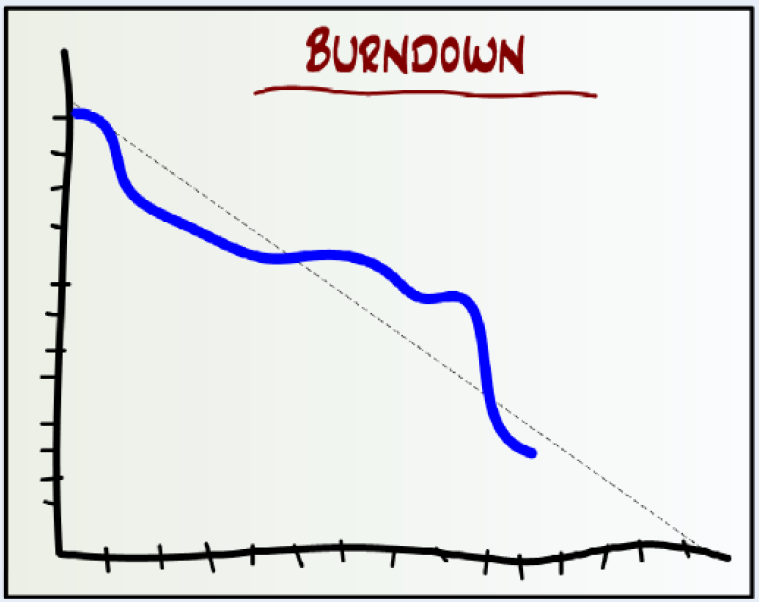
\includegraphics[width=0.55\linewidth]{lifecycle/img/burndownchart}
\caption{Burndown chart (Source: Henrik Kniberg)}
%\caption{Release Burndown Chart showing scope changes
%(Source http://alistair.cockburn.us/)}
\end{figure}
\newslide
% https://www.joelonsoftware.com/2007/10/26/evidence-based-scheduling/
%
And what about Microsoft Project?
Software development guru Joel Spolsky puts it this way:
\begin{quote}
"The trouble with Microsoft Project is that it assumes that you want
to spend a lot of time worrying about dependencies... I've found that
with software, the dependencies are so obvious that it's just not
worth the effort to formally keep track of them."
\end{quote}
Joel continues:
\begin{quote}
Another problem with Project is that it assumes that you're going to
want to be able to press a little button and ''rebalance'' the
schedule... For software, this just doesn't make sense [in
practice]... The bottom line is that Project is designed for building
office buildings, not software.
\end{quote}
Joel is a former Microsoft employee, who worked on both Excel and
Project.  He's not alone in his views. Chris Peters, Microsoft's Vice
President in charge of Office, also said that Microsoft Project is
more appropriate for managing the design of airplanes and buildings,
rather than
software. (\href{http://www.agilekiwi.com/earnedvalue/agile-charts}
{www.agilekiwi.com/earnedvalue/agile-charts})
%
\begin{itemize}
\item Aufwandschätzung mit Story Points (Mike Cohn)
\href{http://www.planningpoker.com/detail.html}
{www.planningpoker.com/detail.html}
\item How to implement Scrum:

\href{http://www.agile-software-development.com/2007/09/how-to-implement-scrum-in-10-easy-steps_20.html}{www.agile-software-development.com/2007/09/how-to-implement-scrum-in-10-easy-steps\_20.html}
\end{itemize}
%
\newpage
%--------------------------------------------------------------------------
%\section*{Projektplanung}
\section{Timeplan}
Axiom: Personen und Monate sind nicht austauschbar.
\begin{enumerate}
\item Calculate the length of a project in months based on the calculated
person months:
\begin{equation}
 D = 2.5 \cdot E ^{\;0.38}
\end{equation}
\item Caclculate the average demand of employees:
\begin{equation}
 P = \frac{E}{D}
\end{equation}
\ifslides
\newpage
\fi
\item Calculation of the effort distribution (in percentage)::\\[1.5ex]
\begin{tabular}{|lccc|}\hline
Software size & small (2 KDL) & medium (32 KDL) & large (128 KDL)\\ \hline
 & & & \\
Design & 19 & 19 & 19 \\
Implementation & 63 & 55 & 51 \\
Integration + Tests & 18 & 26 & 30 \\ \hline
\end{tabular}
\ifslides
\newpage
\fi
\item Refinement of all phases and creation of the predecessor list:
\begin{center}
\begin{tabular}{|l|l|c|c|l|}
\hline
No & Task & Predecessor & Duration & Ressource \\
\hline
1   & Software design &    & 5  & Meier \\
2   & Design approval & 1 & 1 & (Review) \\
3   & Implementation GUI & 2 & 25 & Hilfiker \\
4   & Implementation DB  & 2 & 12 & \ldots   \\
5   & Module test GUI &    3 & 3 & \ldots \\
6   & Module test DB  &    4 & 2 & \ldots \\
7   & Integration   &    5,6 & 2 & \ldots \\
\hline
\end{tabular}
\end{center}
\end{enumerate}

Further development of the model:

\href{http://sunset.usc.edu/csse/research/COCOMOII/cocomo_main.html}
  {sunset.usc.edu/csse/research/COCOMOII/cocomo\_main.html}

\newslide
Calculation software:
\begin{itemize}
\item  COCOMO 81 Intermediate Model Implementation:

  \href{http://sunset.usc.edu/research/COCOMOII/cocomo81_pgm/cocomo81.html}
  {sunset.usc.edu/research/COCOMOII/cocomo81\_pgm/cocomo81.html}

\item COCOMO II with Heuristic Risk Assessment:

  \href{http://sunset.usc.edu/research/COCOMOII/expert_cocomo/expert_cocomo2000.html}{sunset.usc.edu/research/COCOMOII/expert\_cocomo/expert\_cocomo2000.html}
\end{itemize}
\newpage
%------------------------------------------------------------------------------
\subsection{Critical Path Method / Critical Path Analysis}
The critical path method (CPM), or critical path analysis (CPA),
is an algorithm for scheduling a set of project activities.
It is commonly used in conjunction with the program evaluation and
review technique (PERT). A critical path is determined by identifying
the longest stretch of dependent activities and measuring the time
required to complete them from start to finish.\\

\vspace{4mm}

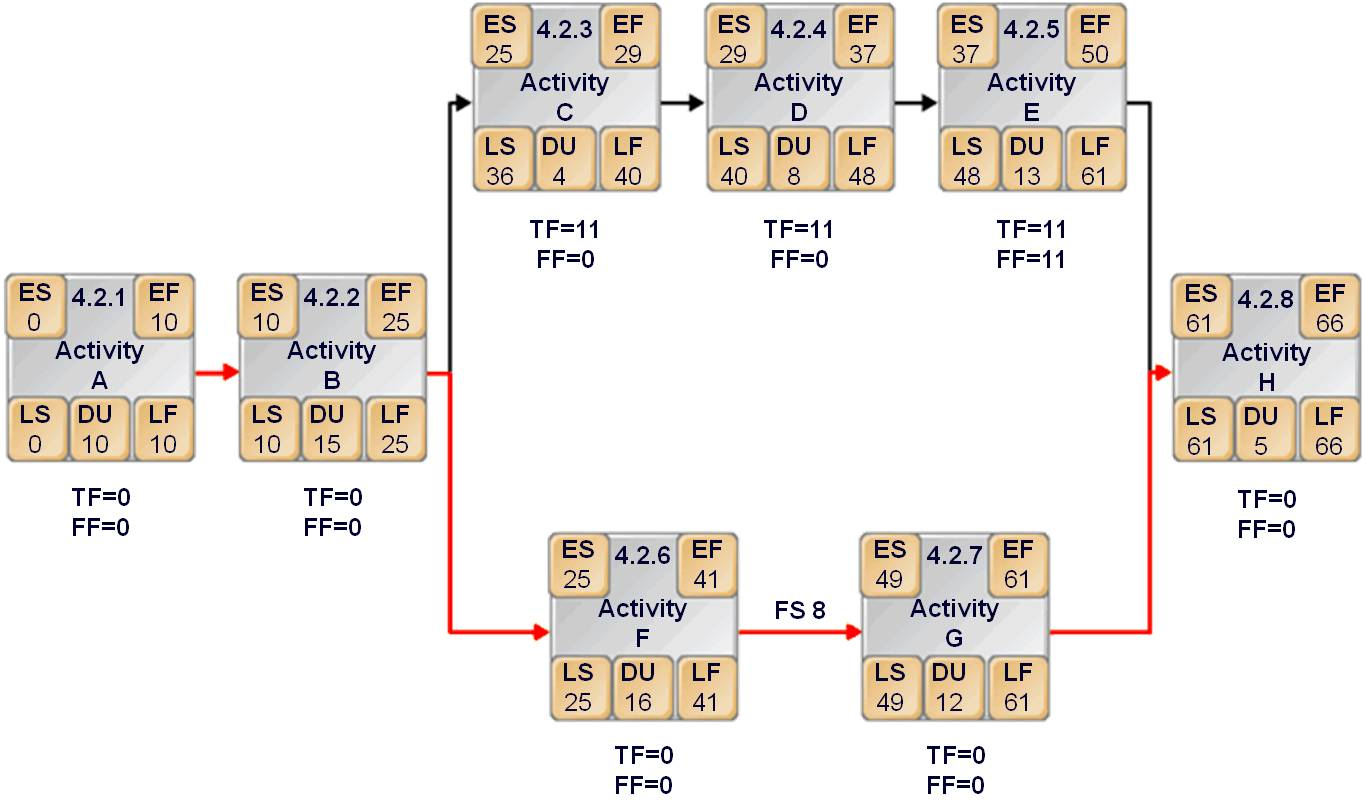
\includegraphics[width=1.0\linewidth]{lifecycle/img/networkdiagram}
%
\newslide
\newpage

\subsection{Gantt charts}
A Gantt chart, or harmonogram, is a type of bar chart that illustrates
a project schedule. This chart lists the tasks to be performed on the
vertical axis, and time intervals on the horizontal axis. The width
of the horizontal bars in the graph shows the duration of each
activity. Gantt charts illustrate the start and finish dates of the
terminal elements and summary elements of a project. Terminal elements
and summary elements constitute the work breakdown structure of the
project. Modern Gantt charts also show the dependency
relationships between activities. (wikipedia.org)
\ifslides
\begin{center}
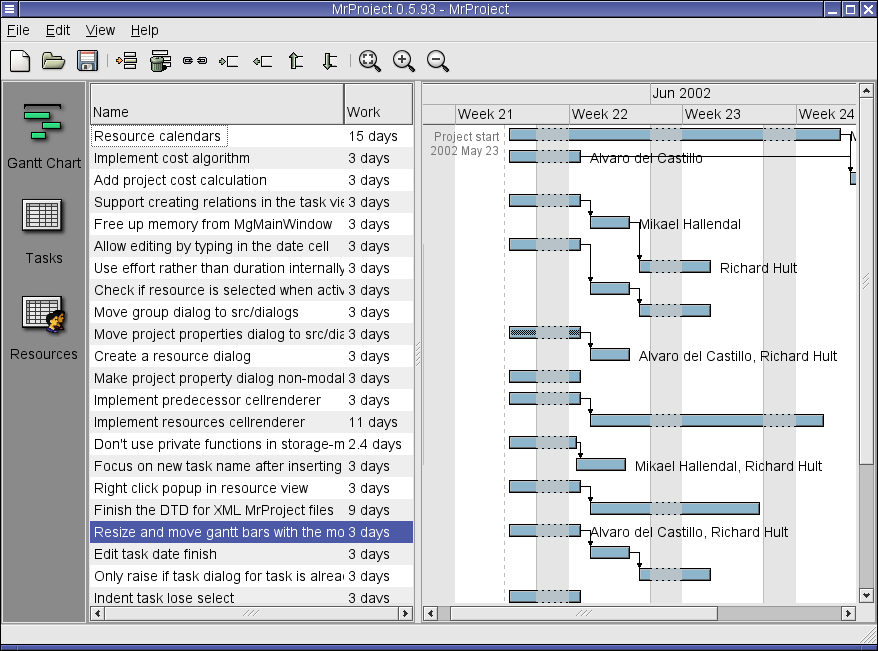
\includegraphics[width=0.75\linewidth]{lifecycle/img/mrproject-gantt}
\end{center}
\else
\vspace{0.5cm}
\begin{figure}[H]
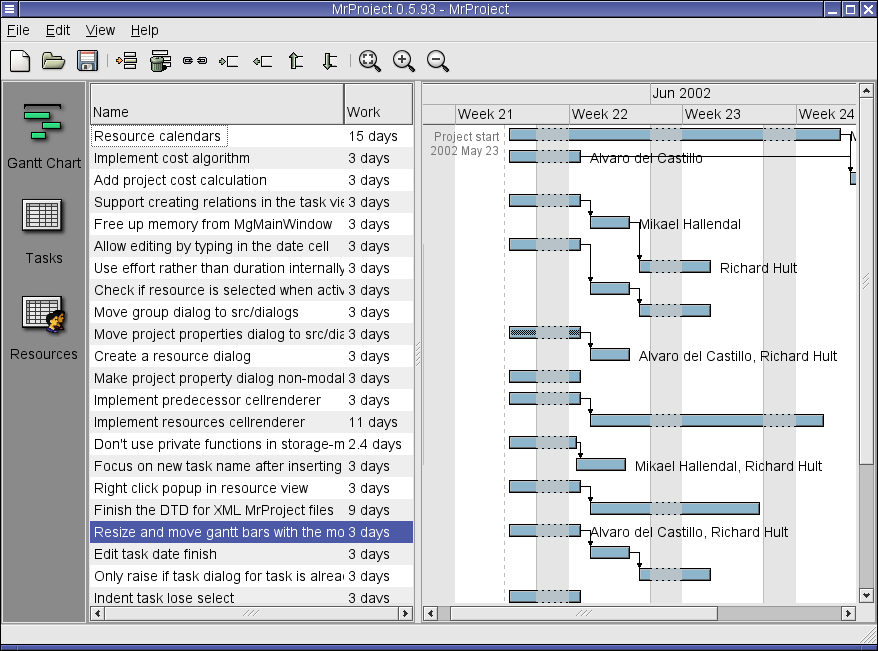
\includegraphics[width=\linewidth]{lifecycle/img/mrproject-gantt}
\caption{Source: \href{http://live.gnome.org/Planner}
               {live.gnome.org/Planner}}
\end{figure}
\fi
%Die Länge der Balken entspricht der Zeitdauer einer Aktivität.

%Bei der Erstellung eines Gantt-Diagrammes ist auf einen sinnvollen
%Detaillierungsgrad zu achten.
\newpage
%------------------------------------------------------------------------------
%\section*{Projektplanung}
\section{Risk Management}
Recognize, analyse and control risks:
%Risiken rechtzeitig erkennen, bewerten und kontrollieren können:
\ifslides
\\{\footnotesize
\else
\\[2ex]
\fi
\begin{tabular}{|l|p{8.5cm}|}
\hline
Risk & Reason \\
\hline
Change of requirements & Scope variations occur when the scope of an iteration
  changes after a timeframe had been agreed upon. Due to the value from
  receiving frequent customer feedback, stakeholders or product owners
  will often ask to vary the scope of a project\\
\hline
Unrealistic planning & Inaccurate estimations occur when the length of a
  project, milestone or iteration is underestimated by the project group.
  Software estimations can cause problems between developers and clients
  because they lead to increase project timeframes, and therefore also
  project expenses. There could also be a problem if people are not
  available due to job change, illness, accident or other reasons.\\
\hline
Missing experience & first usage of a technology, method, tools,
  reduced knowledge of the project area,
  complex SW/HW environment, special requirements, big data,
  high reliability\\
\hline
Improper infrastructure & instable or non-working HW/SW components. Problem with
  component delivery by 3rd party vendor\\
\hline
Financial issue      & Reorganization, incorrect budget estimation,
  project scope expansion, cost overruns\\
\hline
Communication issues & Inadequate support, misunderstanding, conflicts\\
\hline
\end{tabular}
\ifslides
}
\fi
\vspace{0.5cm}

Level of risk:
\begin{equation}
  Risk = Likelihood \cdot Severity
\end{equation}
Project management standards dictate that planning in advance for risks to
the project is a critical success factors.  Each risk should be identified
and ranked on a scale of probability and severity (1-10 or similar) in a
risk log.\\
Once prioritized, there are 5 primary ways to manage your project risks:

\begin{enumerate}
\item Avoidance\\
Although often not possible, this is the easiest way of removing risk from a
project.  It involves the removal of the tasks that contain the risk from the
project.
\item Acceptance\\
On the other end of the spectrum, acceptance involves planning the risk into
the project.  If a better response strategy cannot be identified, accepting
the risk might be sufficient to proceed with the project.
\item Monitor and Prepare\\
Similar to accepting the risk, this response can be used for major risks that
carry a high probability and/or severity, but must be accepted by the project.
It involves the following two things:
\begin{itemize}
\item Creating plans for monitoring the triggers that activate the risk.
\item Building action plans that can be immediately mobilized upon occurrence of the risk.
\end{itemize}
\item Mitigation\\
Since risk is a function of probability and severity, both of these factors
can be scrutinized to reduce the risk of project failure.
\begin{itemize}
\item Probability of occurance:  Take measures to reduce the likelihood of a risk occurring.  This is usually a more preferable option than reducing the severity because it’s better not to experience the risk occurrance in the first place.
\item Severity:  Reduce the impact of the risk on the critical success factors of the project.
\end{itemize}
\item Transference\\
Finally, you can transfer the risk onto another party.  Naturally, this
will usually require some form of trade-off (or cost).  Shifting the
consequence of a risk to a third party is not always easy but is often overlooked.
\end{enumerate}

\newpage
%------------------------------------------------------------------------------
\section{Measurements and Metrics}
With measurements, attributes become quantifiable and measureable:\\[2ex]
%Durch Messungen werden Merkmale quantitativ erfassbar und vergleichbar:\\[2ex]
\begin{tabularx}{\linewidth}{|l|X|}
\hline
Attribute & Measurement \\
\hline
Software size & (LOC) Number of lines of code\\
Complexity & Number of classes, methods, relations\\
Change frequency & Number of changes in a given time frame\\
Fault rate & Number of errors in a given time frame\\
Productivity & Number of lines in a given time frame \\
Effort & Number of working hours \\
\hline
\end{tabularx}
\subsection{Incidents, errors and reliability}
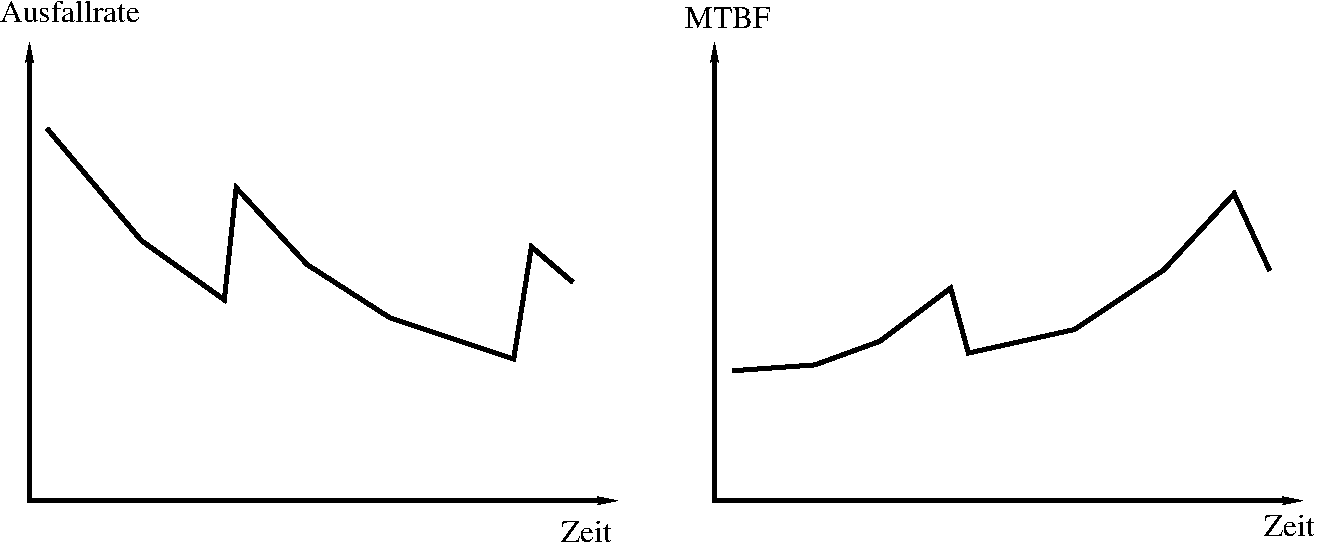
\includegraphics[width=0.8\linewidth]{lifecycle/xfig/failurerate}\\
\ifslides
{\footnotesize
\fi
\begin{tabularx}{\linewidth}{lX}
failure & Deviation of the operating behavior from its requirements \\
fault, bug & Cause of one or more malfunctions \\
error & wrong, incorrect or incomplete implementation \\
reliability & Probability of trouble-free operation during a certain period of time \\
availability & Ratio of the trouble-free operating time to the total operating time \\
\end{tabularx}
\ifslides
}
\fi
\begin{minipage}[t]{0.3\linewidth}
\small
\begin{tabular}{ll}
MTBF & mean time\\
     & between  failures\\
MTTR & mean time\\
     & to repair \\
MTTF & mean time\\
     & to failure\\
\end{tabular}

\end{minipage}
\hfill
\begin{minipage}{0.6\linewidth}
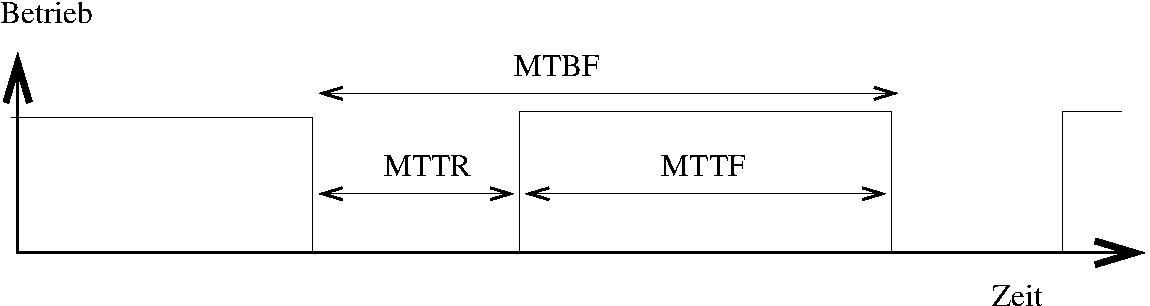
\includegraphics[width=\linewidth]{lifecycle/xfig/mttf-mttr}

{\small
\begin{tabular}{llll}
Nines of     &            \multicolumn{3}{c}{downtime per year}\\
Reliability: &         [h]    &     [min]   &     [sec]\\
\hline
2 9's (99\%)     &  87.6    &   5256.0   &  315360.0 \\
3 9's (99.9\%)    &  8.76   &    525.6   &   31536.0 \\
4 9's (99.99\%)   &  0.876  &     52.56  &    3153.6 \\
%5 9's (99.999%)   & 0.0876   &    5.256  &    315.36\\
%6 9's (99.9999%)   0.00876      0.5256      31.536
%7 9's (99.99999%)  8.76E-4      0.05256      3.1536
%
\end{tabular}
}
\end{minipage}
%
\newpage

\section{Excercise}

\begin{enumerate}
\item What is the critical path for the given task list and what is the duration (of the critical path)?
\begin{tabular}{l|l|l}
Task & Duration (Days) & Predecessor\\
\hline
A & 4 & - (Start)\\
B & 3 & A\\
C & 1 & B\\
D & 5 & - (Start)\\
E & 4 & D\\
F & 6 & E\\
G (end) & 2 & C,F\\
H & 4 & D\\
I (end) & 2 & H
\end{tabular}

\item VLC is a popular video player software. Try to find out how many lines
of code are needed based on the given user interface:\\
\vspace{3mm}
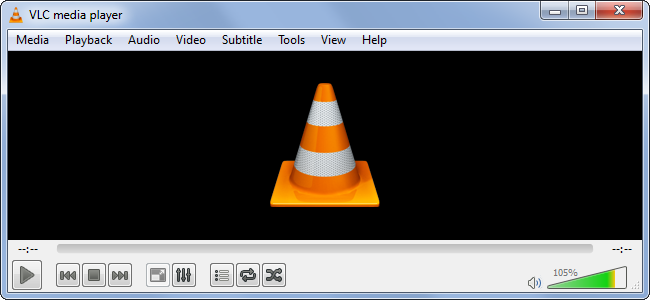
\includegraphics[width=\linewidth]{lifecycle/img/vlc}

\item You are responsible to find out how many person months are needed to
create a simple time recording software. The requirements are the following:

\begin{itemize}
\item The system is a single user system
\item A database is used to store the information
\item The user could add, delete or change an entry
\item An entry contains \emph{date, time, task}
\item A report could be created for a given month. This report will list
a activities for the specified month.
\end{itemize}

\end{enumerate}

%
\chapter{Software Development Life Cycle Models}%\vspace{1cm}
Software development life cycle refers to the process of software development.
The standard for software life cycle processes, describes the development
process as consisting of requirements, design, code, and testing.
There are different approaches to break down the work when developing software
systems. Conceptually, each model provides specific guidance to the
sequencing and repetition of life cycle activities to deliver software systems.

\vspace{3mm}

There is no process that can fit all projects. The most important factors
to choose the best model are the following ones:
\begin{itemize}
\item Project Scope/Size
\item Organizational Cultutre
\item Involved People
\item Criticality
\item Stability
\end{itemize}

\ifslides
\\
\else
%\\[3ex]
\fi
%
%Wir betrachten hier die zwei wichtigsten Vertreter:
\begin{minipage}[t]{0.35\linewidth}
\section{Build and fix model}
no specific procedure
\begin{center}
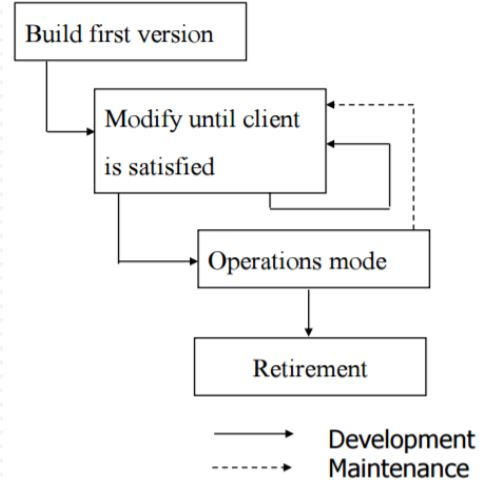
\includegraphics[width=\linewidth]{lifecycle/img/buildandfix.jpg}
\end{center}
\end{minipage}
\hfill
%
\ifslides
\begin{minipage}[t]{0.5\linewidth}
\else
\begin{minipage}[t]{0.5\linewidth}
\fi
\section{Waterfall model}
sequential, fixed, not adaptive
\begin{center}
\ifslides
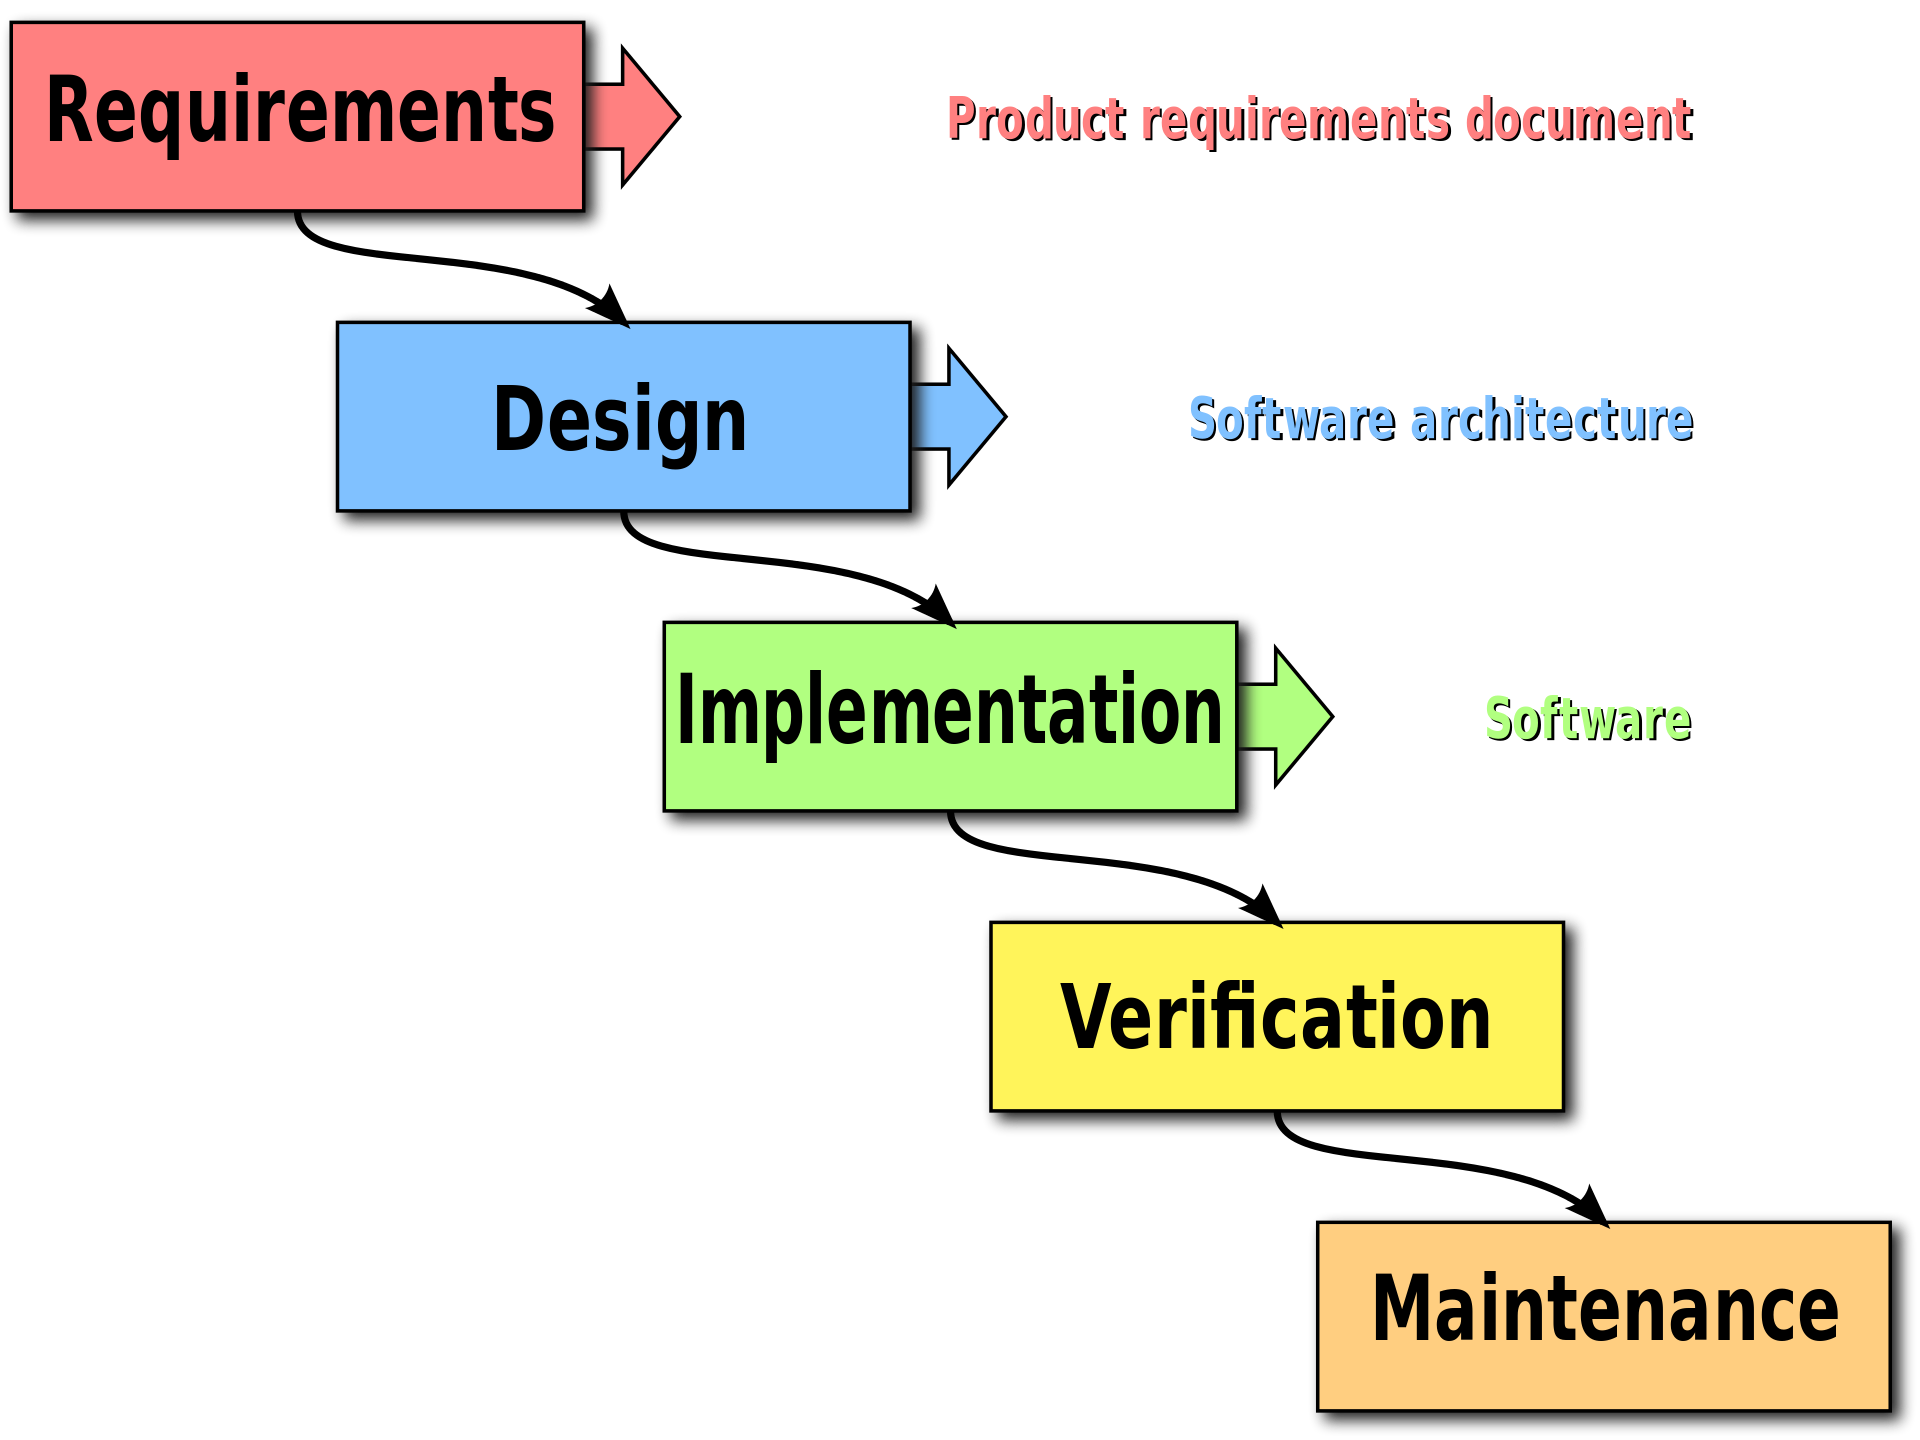
\includegraphics[width=0.8\linewidth]{lifecycle/img/waterfall}
\else
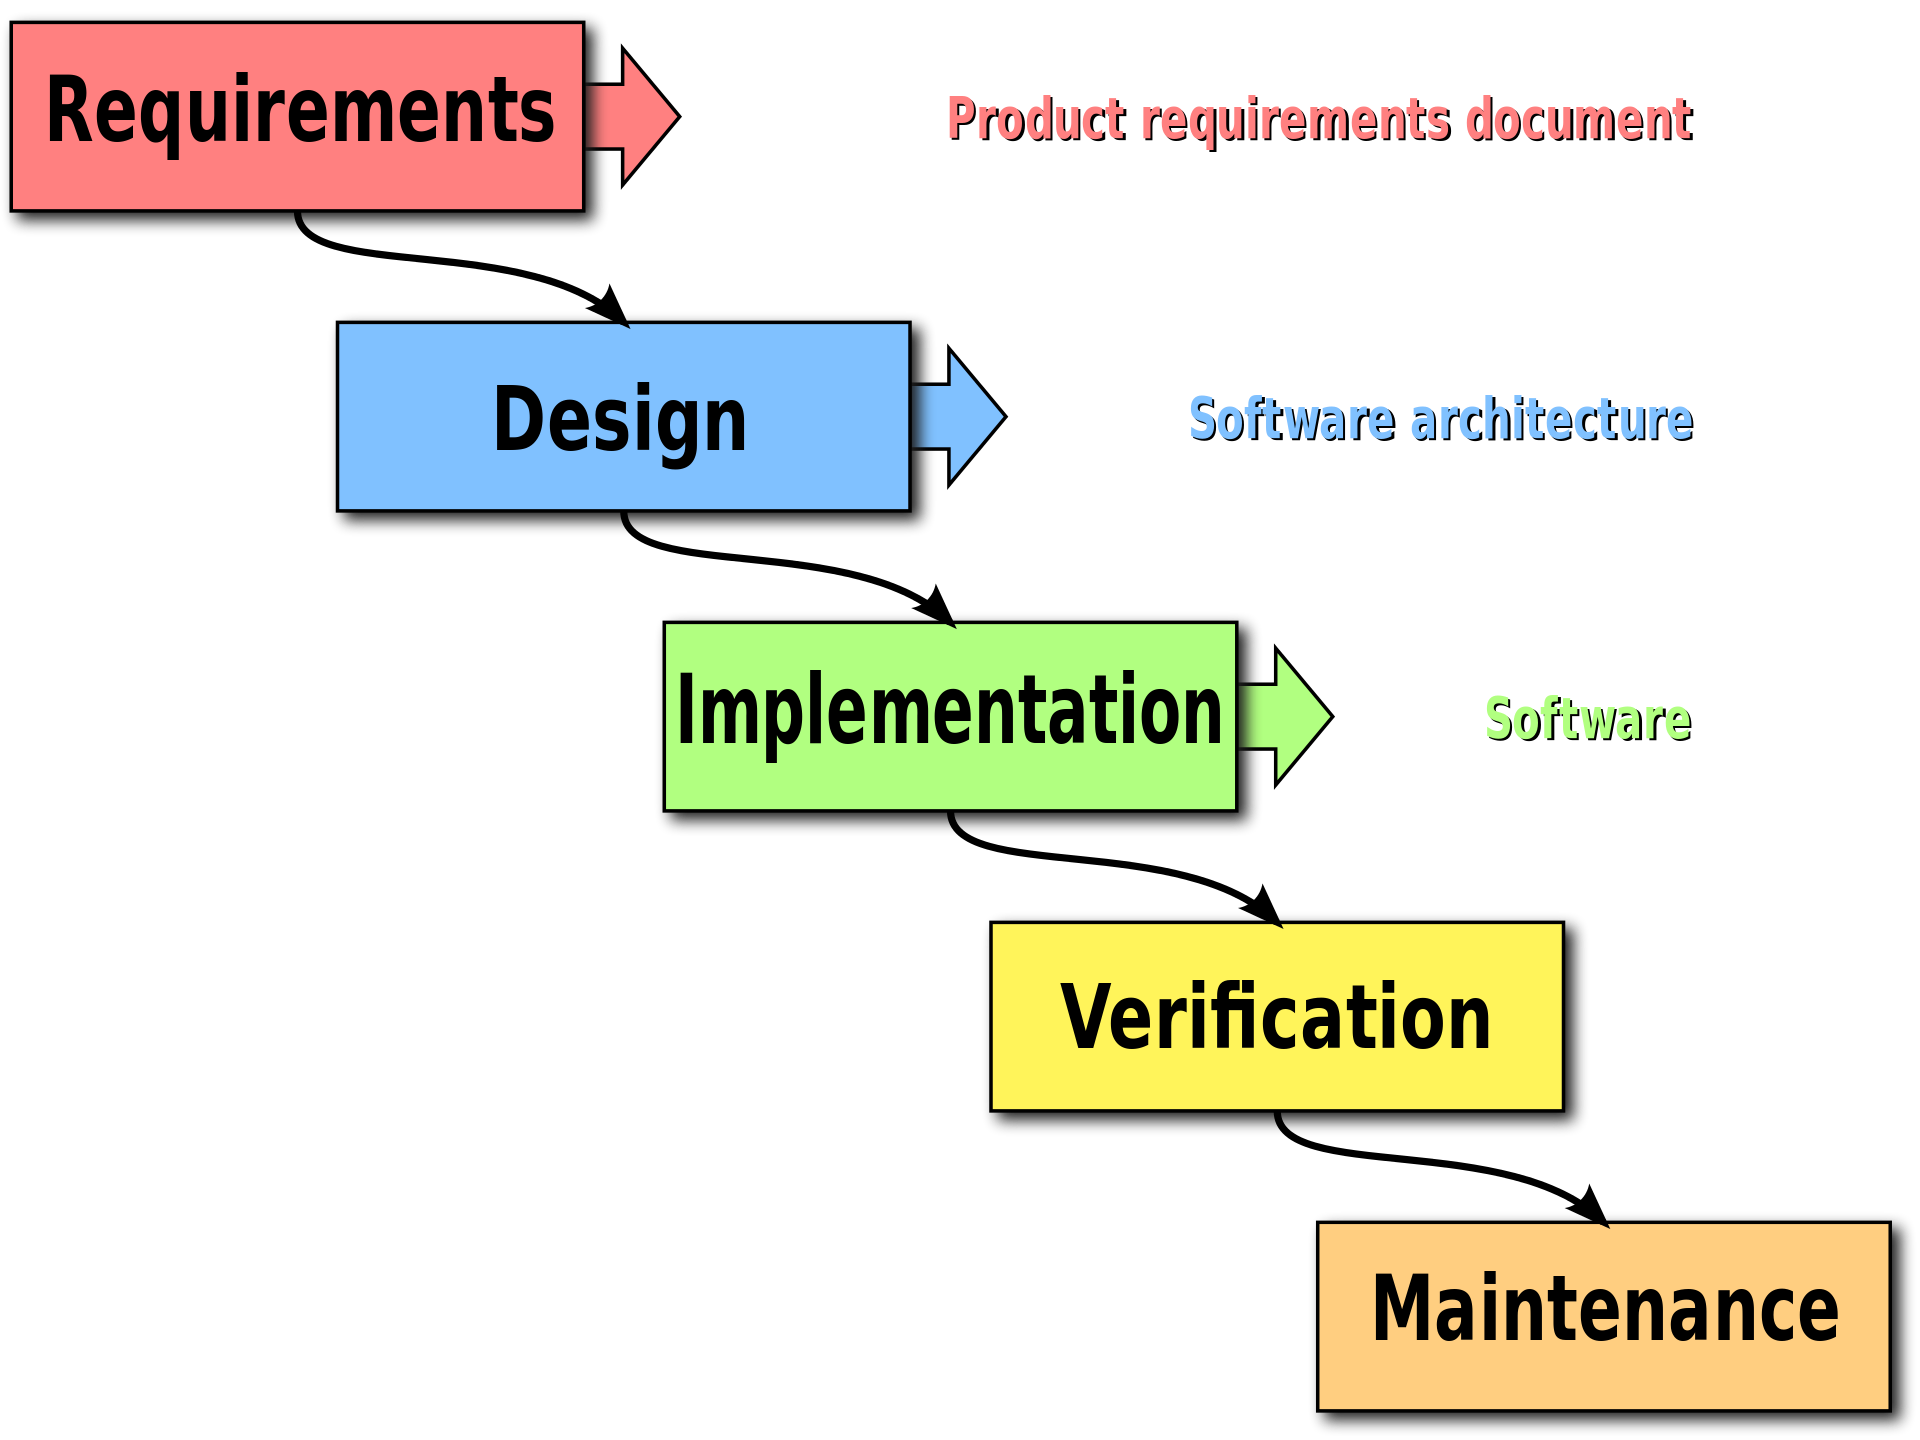
\includegraphics[width=0.8\linewidth]{lifecycle/img/waterfall}
\fi
\end{center}
\end{minipage}
\vspace{1cm}
\newpage
\section{Spiral model}
Risk driven, incremental
%zyklisch, risiko-orientiert
\begin{center}
%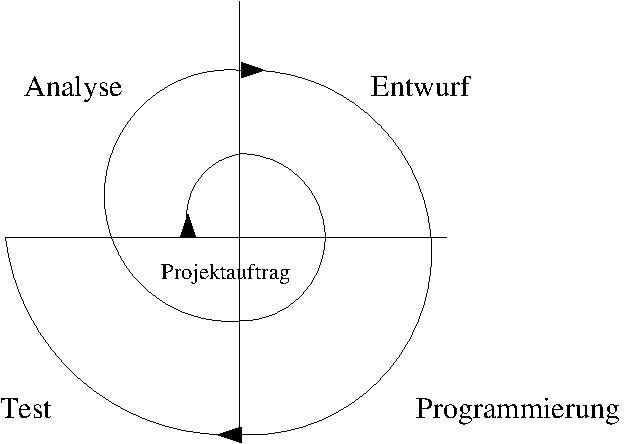
\includegraphics[width=0.6\linewidth]{lifecycle/xfig/spiral}
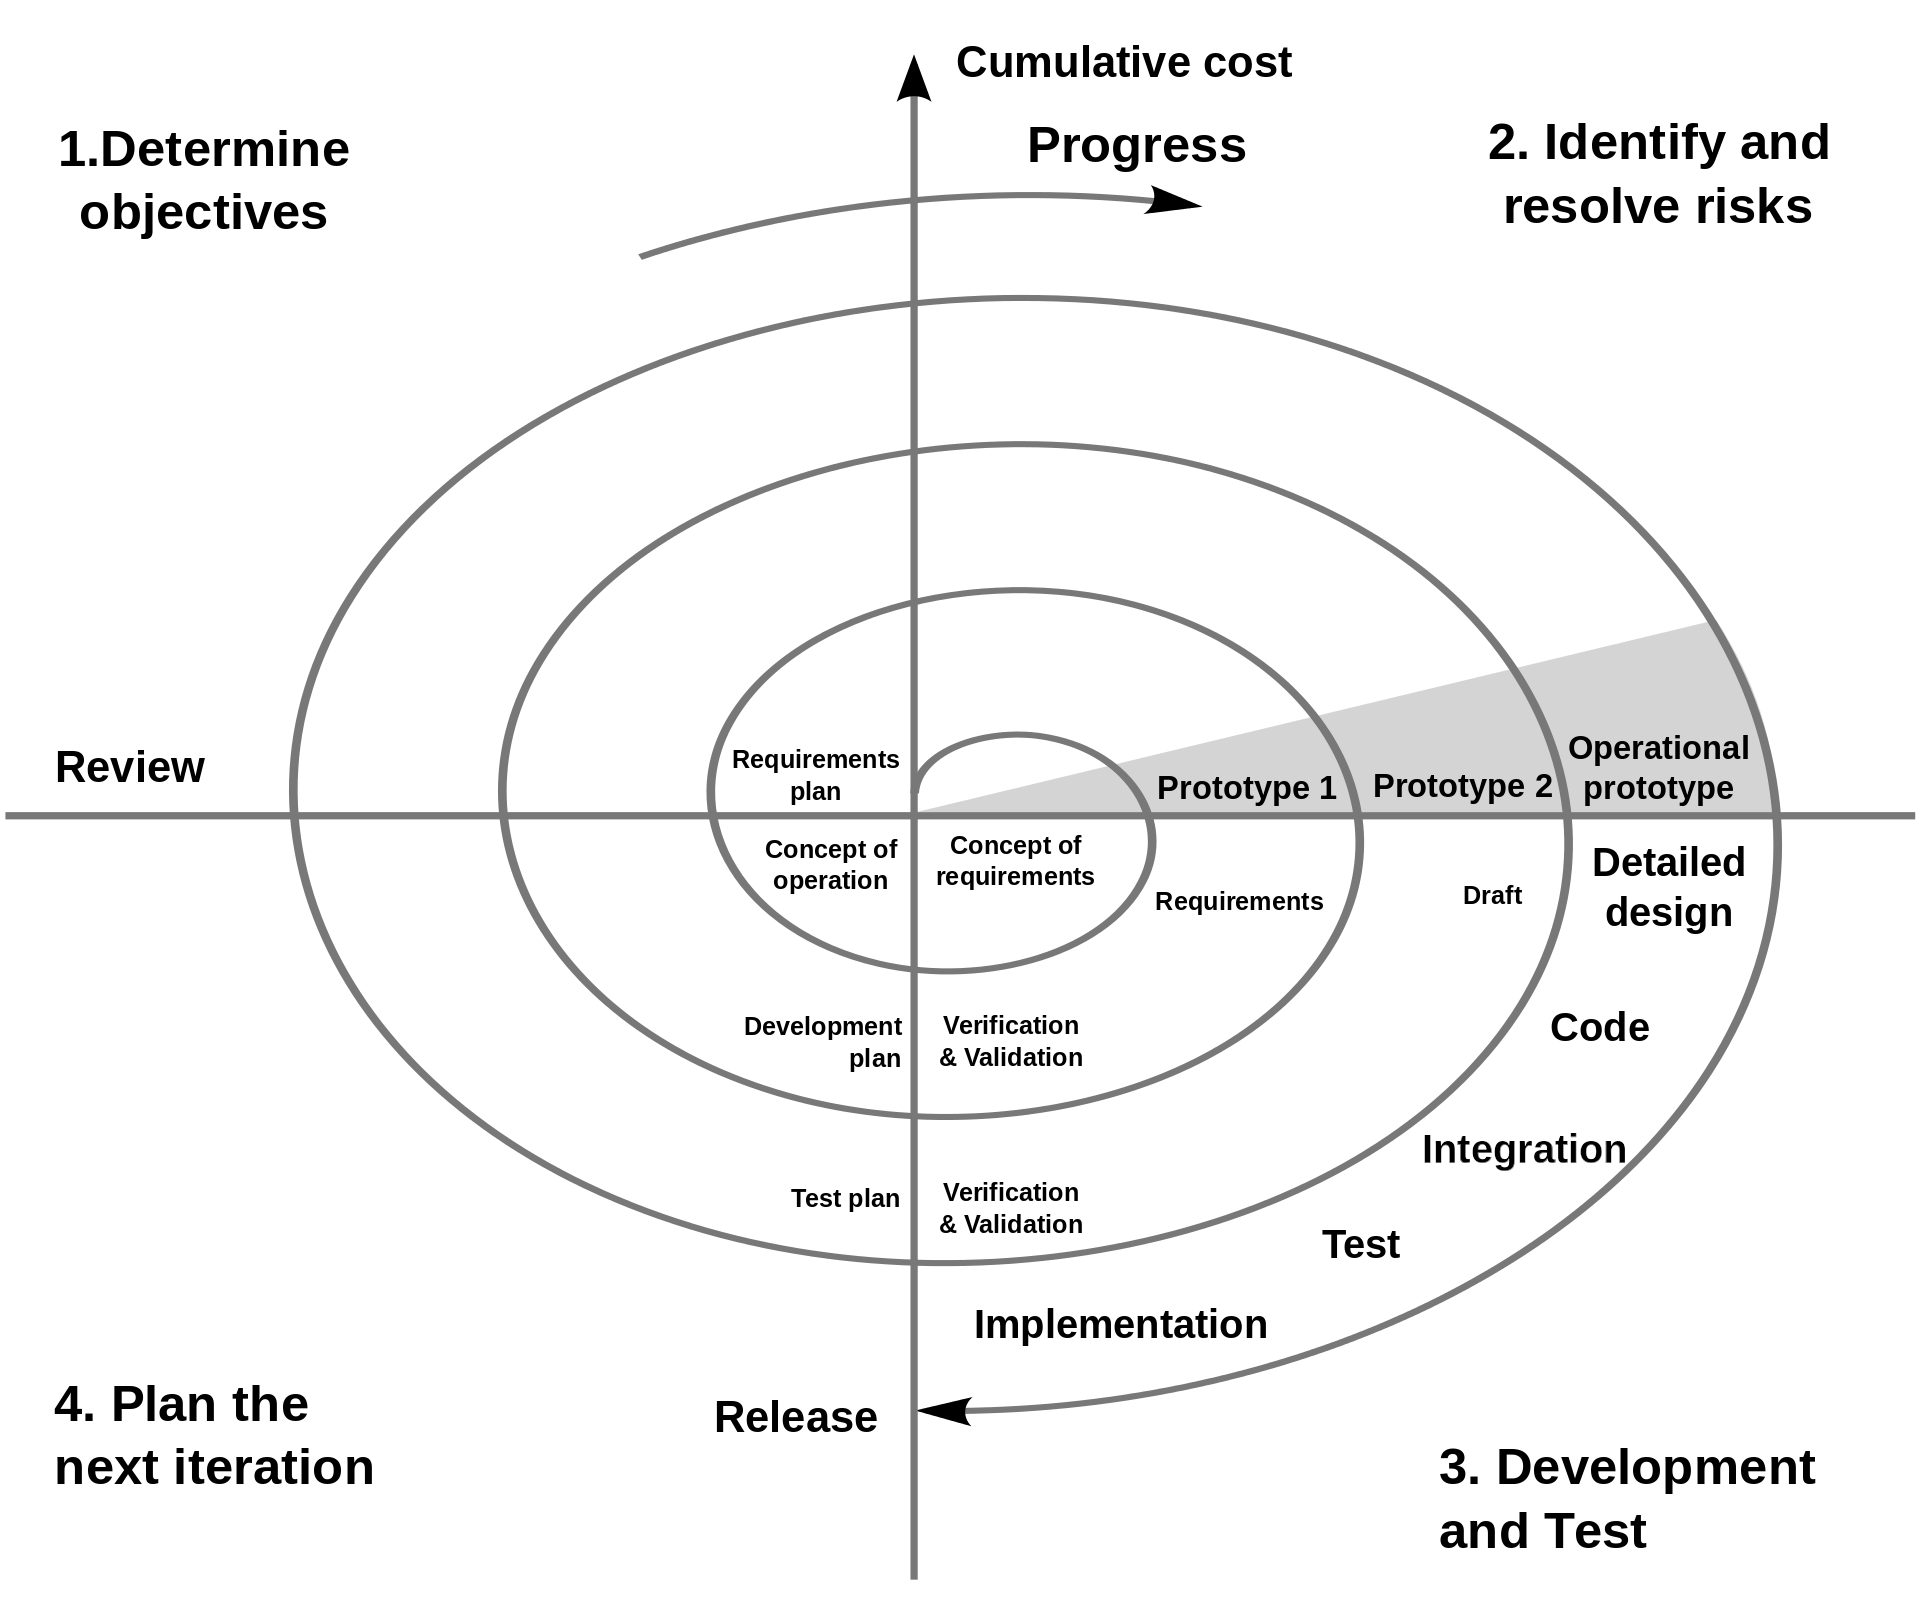
\includegraphics[width=0.6\linewidth]{lifecycle/img/spiralmodel}
\end{center}
%
\section{Hermes}
\ifslides
\else
%Ein offener Standard zur Führung und Abwicklung von Informatikprojekten
%in- und ausserhalb der schweizerischen Bundesverwaltung (seit 1975, letzte
%Überarbeitung/Aktualisierung 2003, neuste Version 5.1, 2014)
HERMES is the project management method for projects in the area of IT,
service and product development, and business organization adjustment.
HERMES supports the steering, management and execution of projects with various
levels of complexity and different features. As a method, HERMES has a clear,
easy-to-understand structure, has a modular design and can be expanded.
 \href{https://www.hermes.admin.ch}{www.hermes.admin.ch}
\begin{figure}[H]
\fi
\begin{center}
\ifslides
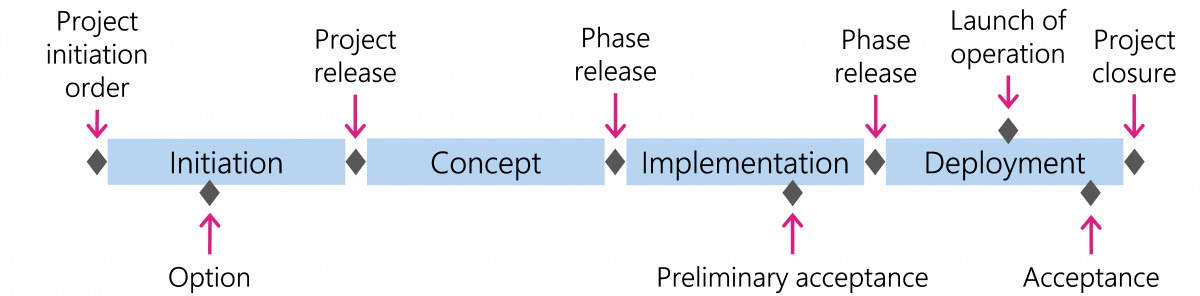
\includegraphics[width=\linewidth]{lifecycle/img/hermes}
\else
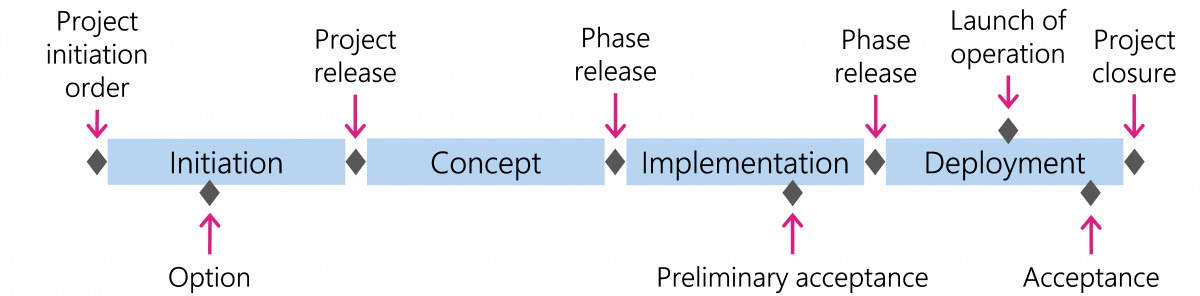
\includegraphics[width=\linewidth]{lifecycle/img/hermes}
\fi
%%\caption{Source: Informatikstrategieorgan des Bundes}
\end{center}
\ifslides
\else
\end{figure}
\fi
%\vspace{2cm}
The phase model forms the backbone of the project. It subdivides the life
cycle of the project and creates the conditions for the project participants
common understanding of the course of the project. The HERMES phase model
consists of four phases:
\begin{description}
\item[Initiation] During the initiation phase, the objectives are defined in
the study and the requirements are worked out in sufficient detail for options
to be developed and evaluated. The project order is created on the basis of the
option selected.
\item[Concept] In the concept phase, the rough requirements documented in the
study are fleshed out and completed as system requirements. Project-specific
solution concepts are designed in detailed studies. They form part of the system
architecture. This describes the system with its processes, functionality,
system components and their integration into the system environment via interfaces.
\item[Implementation] Based on the system architecture, the detailed
specifications are created and the system is developed according to those.
This also includes testing as a prerequisite for the decision on preliminary
acceptance.
\item[Deployment] In the deployment phase, the system is activated and then the
decision on acceptance is made.
\end{description}

\newslide

HERMES offers eight standard scenarios for projects with different characteristics:

\structure{Scenarios}: Anpassung an jeweilige Projektcharakteristiken:
\begin{itemize}
%\item IT-Individualanwendung: Entwicklung und Integration
%\item IT-Standardanwendung: Beschaffung und Integration
%\item IT-Anwendung-Weiterentwicklung
%\item IT-Infrastruktur: Erweiterung, Anpassung
%\item Dienstleistung/Produkt
%\item Organisationsanpassung

\item Service/product
\item Customized IT application
\item Standard IT application
\item Further development of IT application
\item IT infrastructure
\item Organizational adjustment
\item Service/product (agile)
\item Customized IT application (agile)
\end{itemize}

\structure{Modules}: wiederverwerwendbare Bausteine zur Erstellung von Szenarien
\begin{itemize}
%\item Beschaffung
%\item Einführungsorganisation
%\item Entwicklung
%\item Geschäftsorganisation
%\item Informationssicherheit und Datenschutz
%\item IT Betrieb, -Migration, -System
%\item Produkt
%\item Projektführung, -grundlagen, -steuerung
%\item Testen

\item Project steering
\item Project management
\item Agile development
\item Project foundations
\item Business organization
\item Product
\item IT system
\item Procurement
\item Deployment organization
\item Testing
\item IT migration
\item IT operation
\item Information security and data protection
\end{itemize}
Ergänzung: Marketing, Kommunikation, Personalentwicklung, Ausbildung, Strategieentwicklung, Einführung Geschäftsverwaltung
\newslide

\section{V-Modell}
The V-model is a graphical representation of a systems development
lifecycle. It is used to produce rigorous development lifecycle models
and project management models. The key attribute of using a
"V" representation was to require proof that the products from the left-side
of the V were acceptable by the appropriate test and integration
organization implementing the right-side of the V.\\

\vspace{3mm}

\begin{figure}[H]
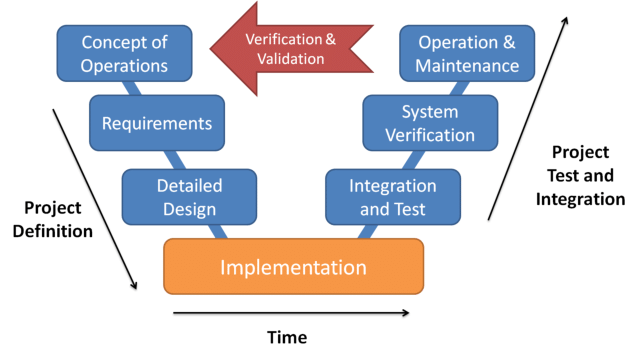
\includegraphics[width=\linewidth]{lifecycle/img/vmodell}
\end{figure}

\subsection{2 Streams}
There are two streams, one stream on each side of the V.
\begin{itemize}
\item Specification Stream\\
User Requirements Specification, Functional Requirement Specification, Design specification
\item Testing Stream\\
Installation qualification, Operational qualification, Performance qualification
\end{itemize}

\subsection{Advantages}
\begin{itemize}
\item The users of the V-model participate in the development and
maintenance of the V-model. A change control board publicly maintains
the V-Model. The change control board meets anywhere from every day to
weekly and processes all change requests received during system development
and test.
\item The V-model provides concrete assistance on how to implement an
activity and its work steps, defining explicitly the events needed to
complete a work step: each activity schema contains instructions,
recommendations and detailed explanations of the activity.
\end{itemize}

\newpage
\section{PRINCE2}
PRINCE2 is a project management method widely adopted around the world,
used by people and organizations from wide-ranging industries and sectors.

It is a flexible method that guides you through the essentials for
managing successful projects, regardless of type or scale. Built
upon seven principles, themes and processes, PRINCE2 can be tailored
to meet your specific requirements.

%1996
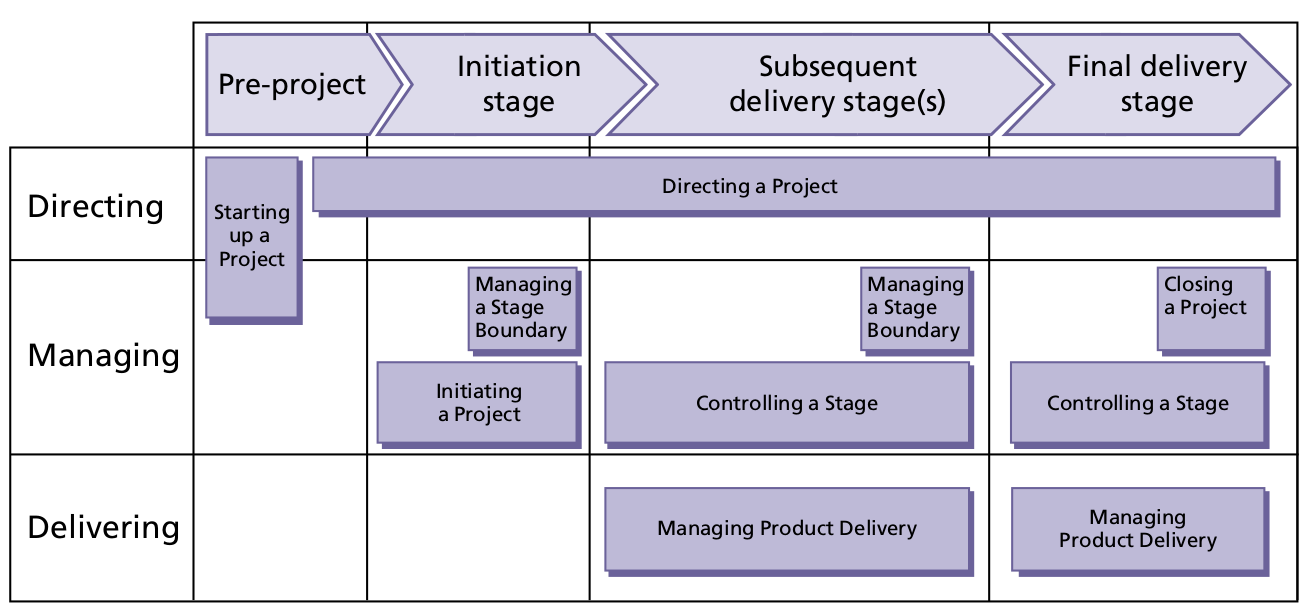
\includegraphics[width=\linewidth]{lifecycle/img/prince2}

\newslide
The Modell includes the following 8 processes:
  (\href{https://www.prince-officialsite.com}{www.prince-officialsite.com})
\begin{description}
\item [1. Directing a Project (DP)]:
Directing a Project runs from the start-up of the project until its
closure. This process is aimed at the Project Board. The Project Board manages
by exception, monitors via reports and controls through a number of decision
points.

The key processes for the Project Board break into four main areas:
\begin{itemize}
\item Initiation (starting the project off on the right foot)
\item Stage boundaries (commitment of more resources after checking results so
  far)
\item Ad hoc direction (monitoring progress, providing advice and guidance,
  reacting to exception situations)
\item Project closure (confirming the project outcome and controlled close).
\end{itemize}
This process does not cover the day-to-day activities of the Project Manager.
%
\ifslides
\newpage
\fi
\item [2. Starting up a Project (SU)]:
This is the first process in PRINCE. It is a pre-project process, designed to
ensure that the pre-requisites for initiating the project are in place. The
process expects the existence of a Project Mandate which defines in high level
terms the reason for the project and what outcome is sought. Starting up a
Project should be very short.

The work of the process is built around the production of three elements:
\begin{itemize}
\item Ensuring that the information required for the project team is available
\item Designing and appointing the Project Management Team
\item Creating the Initiation Stage Plan.
\end{itemize}
%
\ifslides
\newpage
\fi
\item[3. Initiating a Project (IP)]: The objectives of Initiating a Project are to:
  \begin{itemize}
  \item Agree whether or not there is sufficient justification to proceed with
  the project
\item Establish a stable management basis on which to proceed
\item Document and confirm that an acceptable Business Case exists for the
  project
\item Ensure a firm and accepted foundation to the project prior to
  commencement of the work
\item Agree to the commitment of resources for the first stage of the project
\item Enable and encourage the Project Board to take ownership of the project
\item Provide the baseline for the decision-making processes required during
  the project's life
\item Ensure that the investment of time and effort required by the project is
  made wisely, taking account of the risks to the project.
  \end{itemize}
\ifslides
\newpage
\fi
\item[4. Managing Stage Boundaries (SB)]:
This process provides the Project Board with key decision points on whether to
continue with the project or not. The objectives of the process are to:
\begin{itemize}
\item Assure the Project Board that all deliverables planned in the current
  Stage Plan have been completed as defined
\item Provide the information needed for the Project Board to assess the
  continuing viability of the project
\item Provide the Project Board with information needed to approve the current
  stage's completion and authorise the start of the next stage, together with
  its delegated tolerance level
\item Record any measurements or lessons which can help later stages of this
  project and/or other projects.
\end{itemize}
\ifslides
\newpage
\fi
\item [5. Controlling a Stage (CS)]:
This process describes the monitoring and control activities of the Project
Manager involved in ensuring that a stage stays on course and reacts to
unexpected events. The process forms the core of the Project Manager's effort
on the project, being the process which handles day-to-day management of the
project. Throughout a stage there will be a cycle consisting of:
\begin{itemize}
\item Authorising work to be done
\item Gathering progress information about that work
\item Watching for changes
\item Reviewing the situation
\item Reporting
\item Taking any necessary corrective action.
\end{itemize}
This process covers these activities, together with the on-going work of risk
management and change control.
\ifslides
\newpage
\fi
\item [6. Managing Product Delivery (MP)]:
The objective of this process is to ensure that planned products are created
and delivered by:
\begin{itemize}
\item Making certain that work on products allocated to the team is
  effectively authorised and agreed e accepting and checking Work Packages
\item Ensuring that work conforms to the requirements of interfaces identified
  in the Work Package
\item Ensuring that the work is done
\item Assessing work progress and forecasts regularly
\item Ensuring that completed products meet quality criteria
\item Obtaining approval for the completed products.
\end{itemize}
\ifslides
\newpage
\fi
\item [7. Closing a Project (CP)]:
The purpose of this process is to execute a controlled close to the
project. The process covers the Project Manager's work to wrap up the project
either at its end or at premature close. Most of the work is to prepare input
to the Project Board to obtain its confirmation that the project may close.

The objectives of Closing a Project are, therefore, to:
\begin{itemize}
\item Check the extent to which the objectives or aims set out in the Project
  Initiation Document (PID) have been met
\item Confirm the extent of the fulfilment of the Project Initiation Document
  (PID) and the Customer's satisfaction with the deliverables
\item Obtain formal acceptance of the deliverables
\item Ensure to what extent all expected products have been handed over and
  accepted by the Customer
\item Confirm that maintenance and operation arrangements are in place (where
  appropriate)
\item Make any recommendations for follow-on actions
\item Capture lessons resulting from the project and complete the Lessons
  Learned Report
\item Prepare an End Project Report
\item Notify the host organisation of the intention to disband the project
  organisation and resources.
\end{itemize}
\ifslides
\newpage
\fi
\item [8. Planning (PL)]
Planning is a repeatable process, and plays an important role in other
processes, main ones being:
\begin{itemize}
\item Planning an Initiation Stage (SL16)
\item Planning a Project (IP2)
\item Planning a Stage (SB1)
\item Producing an Exception Plan (SB6).
\end{itemize}
PRINCE provides a product-based start to the planning activity. It also provides planning framework which can be applied to any type of project. This involves:
\begin{itemize}
\item Establishing what products are needed
\item Determining the sequence in which each product should be produced
\item Defining the form and content of each product
\item Resolving what activities are necessary for their creation and delivery.
\end{itemize}
\end{description}
\ifslides
\newpage
\fi
Managers using PRINCE are able to...
\begin{itemize}
\item Establish terms of reference as a pre-requisite to the start of a
  project
\item Use a defined structure for delegation, authority and communication
\item Divide the project into manageable stages for more accurate planning
\item Ensure resource commitment from management is part of any approval to
  proceed
\item Provide regular but brief management reports
\item Keep meetings with management and stakeholders to a minimum but at the
  vital points in the project.
\end{itemize}
\ifslides
\newpage
\fi
Those who will be directly involved with using the results of a project are able to...
\begin{itemize}
\item Participate in all the decision-making on a project
\item If desired, be fully involved in day-to-day progress
\item Provide quality checks throughout the project and ensure their
\item requirements are being adequately satisfied.
\end{itemize}
For senior management PRINCE uses the 'management by exception' concept. They
are kept fully informed of the project status without having to attend
regular, time-consuming meetings.
\ifslides
\else
\newpage
\fi
\section{Unified-Process}
\ifslides
%Rational Corp (Ivar Jacobson)
\else
The Unified Process is not simply a process, but rather an extensible
framework which should be customized for specific organizations or
projects. The Rational Unified Process is, similarly, a customizable
framework. As a result, it is often impossible to say whether a
refinement of the process was derived from UP or from RUP, and so
the names tend to be used interchangeably.\\

The name Unified Process as opposed to Rational Unified Process is
generally used to describe the generic process, including those elements
which are common to most refinements. The Unified Process name is also
used to avoid potential issues of trademark infringement since Rational
Unified Process and RUP are trademarks of IBM.
\fi
\begin{center}
\ifslides
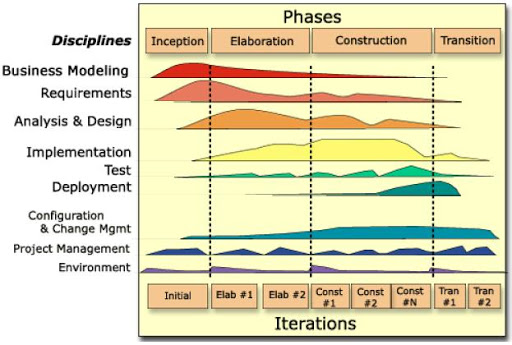
\includegraphics[width=0.8\linewidth]{lifecycle/img/unifiedprocess.jpg}
\else
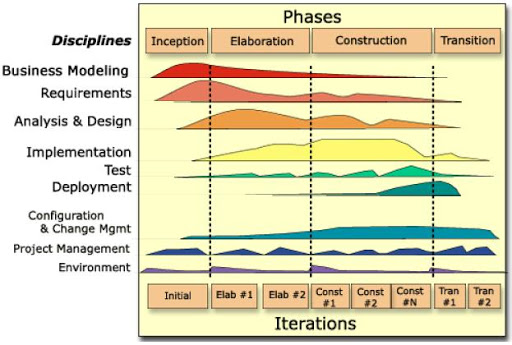
\includegraphics[width=0.9\linewidth]{lifecycle/img/unifiedprocess.jpg}
\fi
\end{center}
\vspace{1.5cm}

\begin{description}
\item[Use-Case-Driven]:\\
  Use case driven means that use cases are used as a primary artifact for
  establishing the desired behavior of the system, for verifying and
  validating the system's architecture, for testing, and for communicating
  among the stakeholders of the project.
\item[Architecture-centric]:\\
  Architecture-centric means that a system's architecture is used as a
  primary artifact for conceptualizing, constructing, managing, and
  evolving the system under development.
\item[Iterative and incremental]:\\
  An iterative process is one that involves managing a stream of
  executable releases. An incremental process is one that involves
  the continuous integration of the system's architecture to produce
  these releases, with each new release embodying incremental improvements
  over the other. Together, an iterative and incremental process is
  risk-driven, meaning that each new release is focused on attacking and
  reducing the most significant risks to the success of the project.
\end{description}
\newpage
\subsection{Phases}
\begin{description}
\item[Inception]:\\
  The idea for the project is stated. The development team determines
  if the project is worth pursuing and what resources will be needed.
\item[Elaboration]:\\
  The project's architecture and required resources are further evaluated.
  Developers consider possible applications of the software and costs
  associated with the development.
\item[Construction]:\\
  The project is developed and completed. The software is designed,
  written, and tested.
\item[Transition]:\\
 The software is released to the public. Final adjustments or updates are
 made based on feedback from end users.
 The Transition phase also includes system conversions and user training.
\end{description}

\subsection{Workflows}
\begin{description}
\item[Business Modelling]:\\
  During this workflow, the business context (scope) of the project should be
  outlined.
\item[Requirements]:\\
  Used to define all potential requirements of the project, throughout the
  software development life cycle.
\item[Analysis and Design]:\\
  Once the requirements workflow is complete, the analysis and design phase
  takes those requirements and transforms them into a design that can be
  properly implemented.
\item[Implementation]:\\
  This is where the majority of actual coding takes place, implementing and
  organizing all the code into layers that make up the whole of the system.
\item[Test]:\\
  Testing of all kinds takes place within this workflow.
\item[Deployment]:\\
  Finally, the deployment workflow constitutes the entire delivery and
  release process, ensuring that the software reaches the customer as expected.
\item[Configuration Management]:\\
Used to describe the various artifacts produced by the development team,
ideally ensuring that there is minimal overlap or wasted efforts performing
similar activities that result in identical or conflicting artifacts.
\item[Project Management]:\\
Where all activities dealing with project management take place, from pushing
design objectives to managing risk to overcoming delivery constraints.
\item[Environment]:\\
Finally, this workflow handles the setup and management of all software
development environments throughout the team, including the processes,
as well as the tools, that are to be used throughout the software
development life cycle.

\end{description}
%%
\newpage
\section{Extreme Programming (XP)}
Extreme programming (XP) is a software development methodology which is
intended to improve software quality and responsiveness to changing customer
requirements. As a type of agile software development,
it advocates frequent "releases" in short development cycles, which is
intended to improve productivity and introduce checkpoints at which new
customer requirements can be adopted. \href{https://www.extremeprogramming.org}
{www.extremeprogramming.org}
\begin{center}
\ifslides
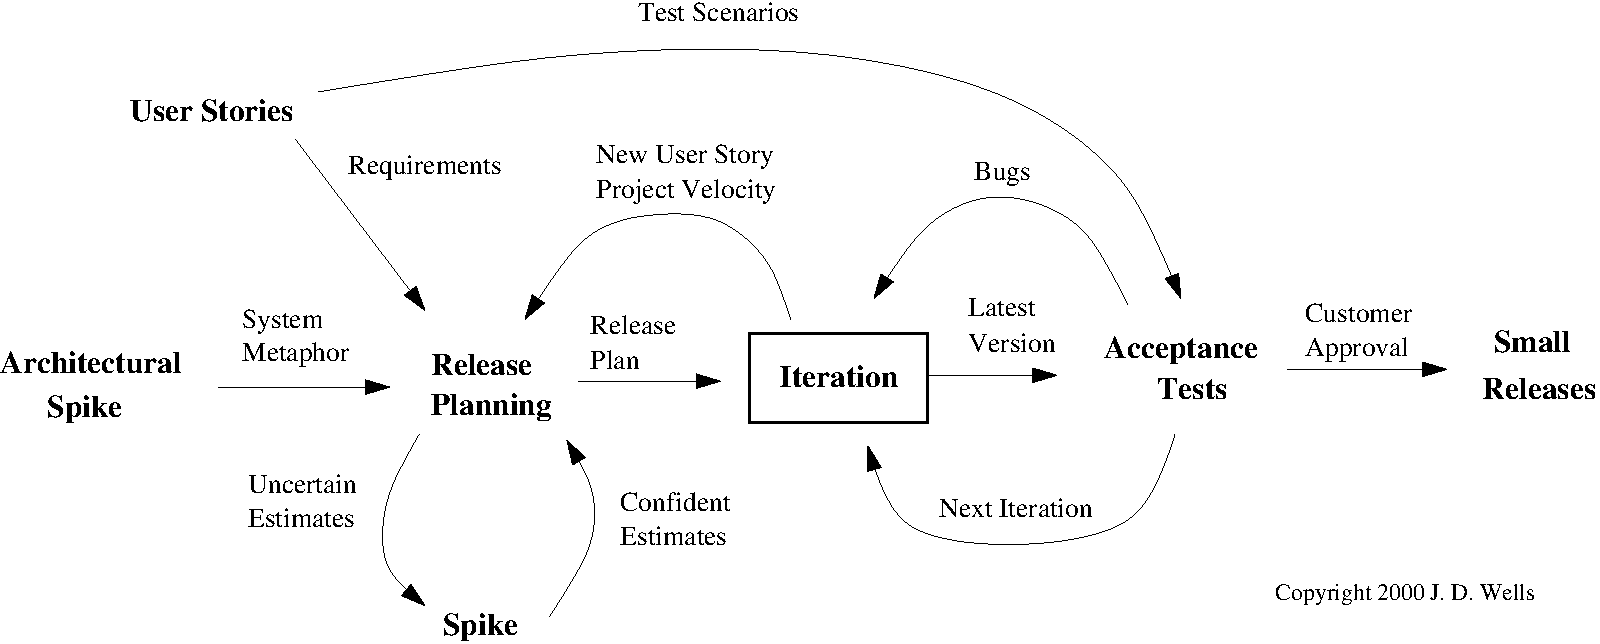
\includegraphics[width=0.9\linewidth]{lifecycle/xfig/xp-project}
\else
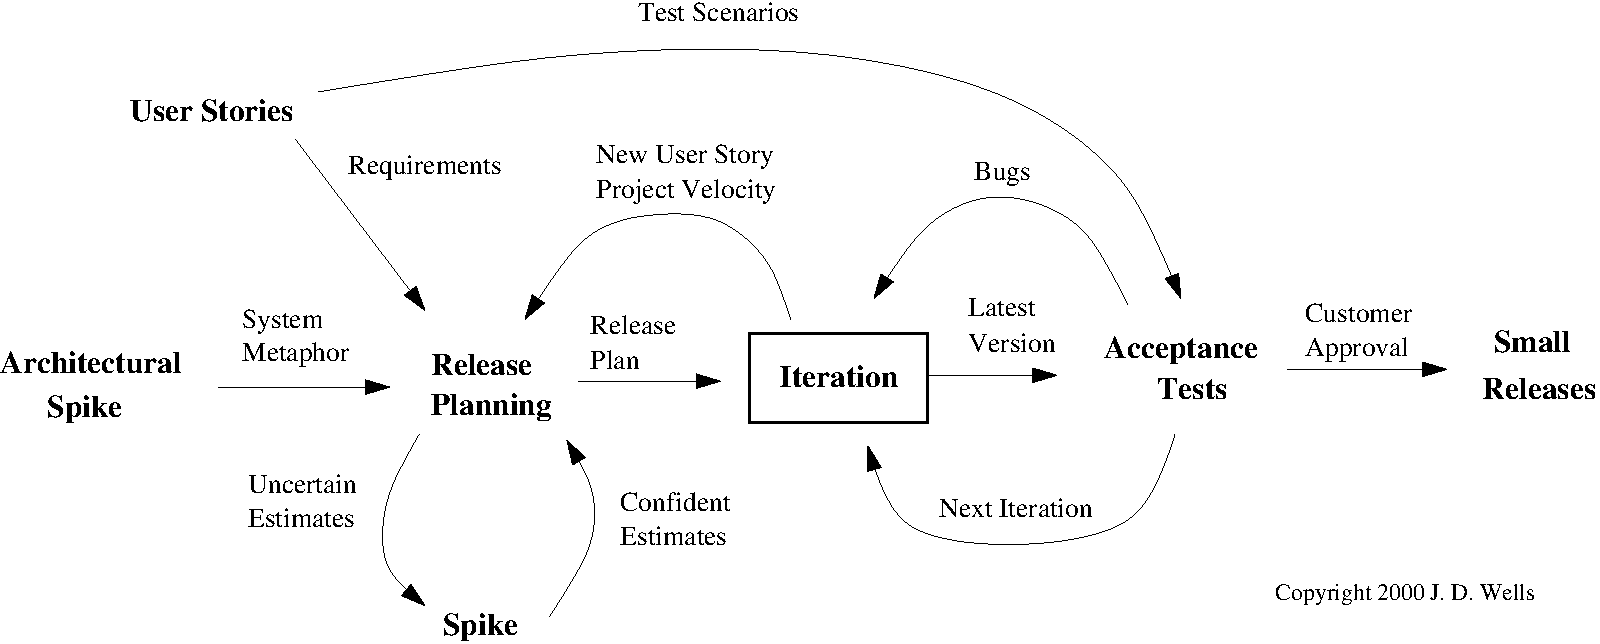
\includegraphics[width=0.8\linewidth]{lifecycle/xfig/xp-project}
\fi
\end{center}
%\section*{Extreme-Programming Grundsätze}

\subsection{Values}
Extreme Programming has simple rules that are based on 5 values:

\begin{description}
\item [Communication]:\\
Everyone on a team works jointly at every stage of the project.
\item  [Simplicity]:\\
Developers strive to write simple code bringing more value to a product, as it
saves time and efforts.
\item [Feedback]:\\
Team members deliver software frequently, get feedback about it, and improve a
product according to the new requirements.
\item [Respect]:\\
Every person assigned to a project contributes to a common goal.
\item [Courage]:\\
Programmers objectively evaluate their own results without making excuses and
are always ready to respond to changes.
\end{description}


\subsection{Principles}
Most researches link XP with the following 5 principles:

\begin{description}
\item [Rapid feedback]:\\
Team members understand the given feedback and react to it right away.
\item [Assumed simplicity]:\\
Developers need to focus on the job that is important at the moment and
follow YAGNI (You Ain't Gonna Need It) and DRY (Don't Repeat Yourself)
principles.
\item [Incremental changes]:\\
Small changes made to a product step by step work better than big ones made at
once.
\item [Embracing change]:\\
If a client thinks a product needs to be changed, programmers should support
this decision and plan how to implement new requirements.
\item [Quality work]:\\
A team that works well, makes a valuable product and feels proud of it.
\end{description}


\subsection{12 Practices}
XP suggests using 12 practices while developing software.

\begin{description}
\item [Test-Driven Development]:
\item [The Planning Game]:
\item [On-site Customer]:
\item [Pair Programming]:
\item [Code Refactoring]
\item [Continuous Integration]
\item [Small Releases]
\item [Simple Design]
\item [Coding Standards]
\item [Collective Code Ownership]
\item [System Metaphor]
\item [Work Condition]
\end{description}
%
\newpage
\subsection{User Story vs Use Case}
A \textbf{user story} is a short description of something that your customer will
do when they come to your website or use your application/software,
focused on the value or result they get from doing this thing. They are
written from the point of view of a person using your website or application,
and written in the language that your customers would use.\\

\newslide
Examples (\href{https://www.agilemodeling.com/artifacts/userStory.htm}
     {www.agilemodeling.com/artifacts/userStory.htm}):
\begin{itemize}
\item Students can purchase monthly parking passes online.
\item Parking passes can be paid via credit cards.
\item Parking passes can be paid via PayPal ™.
\item Professors can input student marks.
\item Students can obtain their current seminar schedule.
\item Students can order official transcripts.
\item Students can only enroll in seminars for which they have prerequisites.
\item Transcripts will be available online via a standard browser.
\end{itemize}

A \textbf{user story} is usually written using the format canonised by Mike Cohn:
\emph{As an [actor] I want [action] so that [achievement]}.\\
So, for example: \emph{As a Flickr member, I want to set different privacy levels
on my photos, so I can control who sees which of my photos}.\\


A \textbf{use case} is a description of a set of interactions between a
system and and one or more actors (where actor can be people, or other
systems: for example, both online shoppers and PayPal can be actors).
They are usually created as documents, and generally include this kind
of information:

\ifslides
\else
\begin{tabularx}{\linewidth}{lX}
%\begin{tabular}{|l|l|}
  \toprule % booktabs package
  Title & Name of use case \\
  \midrule
    Description & some short text describing the scope.\\
  \midrule
    Actor(s) & person(s) who interact with this particular use case. \\
  \midrule
    Precondition & anything that this use case can assume to be true
                        prior to beginning it's life cycle.\\
  \midrule
    Success scenario & a sequence of steps describing correct flow of
         events that take place.\\
  \midrule
  Extensions & flow of application when it deviates from success scenario's flow:
    \begin{itemize}
    \item
      Alternate flows - other options of correct flow
    \item
      Exception flows - flow of events for when things go wrong
    \end{itemize}\\
  \midrule
        Post condition &  state of application after everything is done\\
        \bottomrule
\end{tabularx}\\[2ex]
\fi

%
\subsection{INVEST (Bill Wake)}
\begin{tabularx}{\linewidth}{l|l|X}
  I & Independent &The user story should be self-contained, in a way that there is no inherent dependency on another user story. \\
  N & Negotiable & User stories, up until they are part of an iteration, can always be changed and rewritten.\\
  V & Valuable & A user story must deliver value to the end user.\\
  E & Estimable & You must always be able to estimate the size of a user story.\\
  S & Small & User stories should not be so big as to become impossible to plan/task/prioritize with a certain level of certainty.\\
  T & Testable & The user story or its related description must provide the necessary information to make test development possible.\\
\end{tabularx}
\newpage
\section{Scrum}
Scrum (Rugby: Gedränge) ist ein agiles Vorgehensmodell für die
Entwicklung komplexer Softwaresysteme. Ursprünglich von Hirotaka
Takeuchi und Ikujiro Nonaka beschrieben, wurde es einige Jahre später von
Jeff Sutherland und Ken Schwaber in Firmen eingesetzt und als Referenz
an ein Rugby-Team

.. tries to go to the distance as a unit, passing the ball back and forth

Scrum genannt.

\newslide
Der Scrum-Prozess beginnt mit der Zusammenstellung der Anforderungen
in Form von User Stories,
was hier als ``Product Backlog'' bezeichnet wird. Für die
Implementierung wählt das Team, welches üblicherweise aus 5-9
Entwicklern besteht, gemeinsam mit dem Kunden (dem Product
Owner) einen Satz von Anforderungen aus, die für die nächste Iteration
wichtig und sinnvoll sind. Dieser Satz wird ``Sprint Backlog''
genannt.
Er wird
getrennt vom Product Backlog verwaltet, da sich während einer
Iteration die Anforderungen ändern können. Dadurch entsteht eine
 Verbindlichkeit: die Entwickler lernen Aufwände besser zu
schätzen und Zusagen einzuhalten und die Kunden konkrete und
relevante Anforderungen zu stellen.
\begin{figure}[H]
\begin{center}
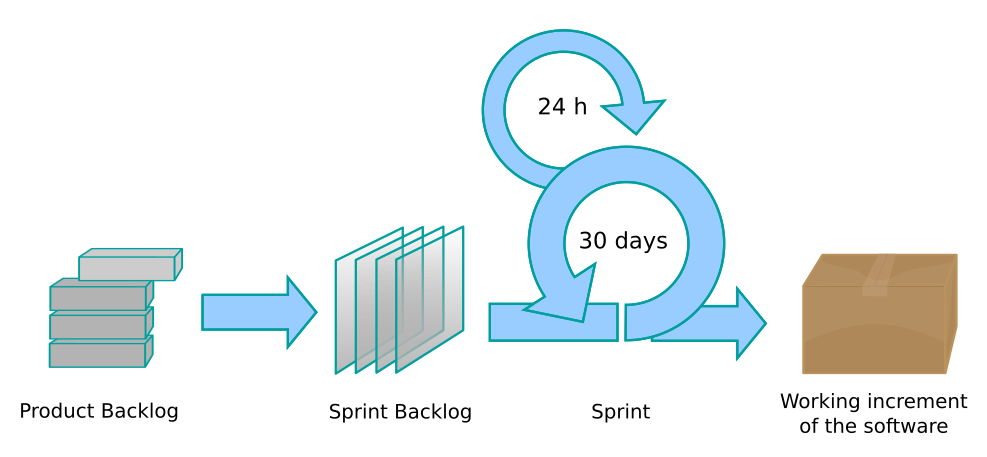
\includegraphics[width=\linewidth]{lifecycle/img/scrum_process}
\caption{Der Scrum-Prozess (Source: Wikipedia)}
\end{center}
\end{figure}
Ein Sprint dauert in der Regel etwa 15 - 30 Tage. Nach dieser Periode
sollte jeweils ein ausführbarer Release zur Verfügung stehen.

Zu Beginn eines Sprints werden die ausgewählten User Stories
in ein mehrspaltiges Taskboard (Sprint Backlog)
übertragen und in einzelne Tasks aufgeteilt:
Design, Implementierung, Test und Dokumentation. Die Tasks werden
in die Spalte ``zu erledigen'' (To Do) platziert. Im Laufe des Sprints
werden die einzelnen Tasks abgearbeitet, wobei die jeweilige Karte in
die entsprechende Spalte verschoben wird, um so den Projektfortschritt
zu dokumentieren.
\begin{figure}[H]
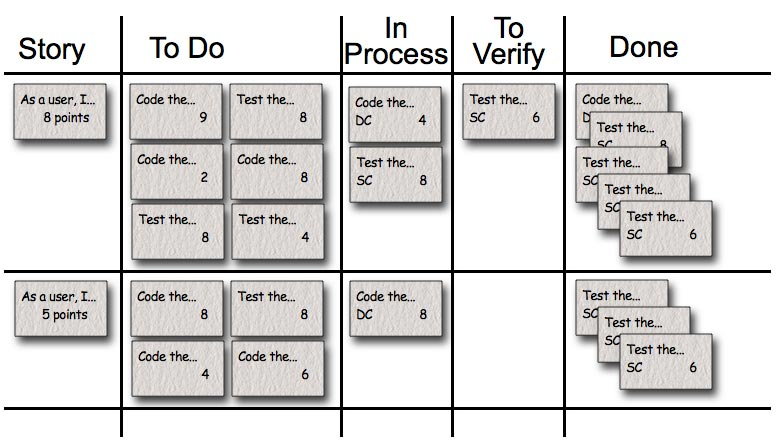
\includegraphics[width=\linewidth]{lifecycle/img/MockedTaskBoard}
\caption{Ein Scrum Taskboard (Source: www.mountaingoatsoftware.com)}
\end{figure}
%\newslide
Die Teilnehmer eines Scrum-Projektes werden in Pigs und Chicken
eingeteilt:
\begin{figure}[H]
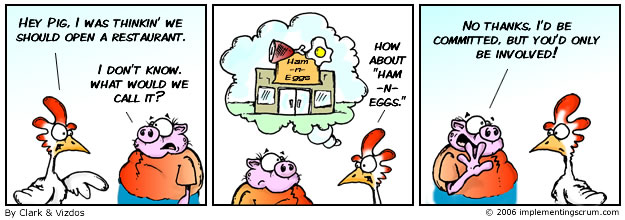
\includegraphics[width=\linewidth]{lifecycle/img/060911-scrumtoon}
\caption{Pigs und Chicken (Source: www.implementingscrum.com)}
\end{figure}
Als Pigs bezeichnet man Teilnehmer, die konkrete Verpflichtungen eingehen
(commit), während Chicken weniger direkt involvierte Teilnehmer sind
(User, Kunden, Anbieter, Manager \ldots).

In täglich durchgeführten Besprechungen (Daily Scrum) wird der
Kontext des aktuellen Tages festgelegt. Alle sind eingeladen daran
teilzunehmen aber nur ``Pigs'' dürfen sich äussern. Dabei geht
es im wesentlichen um die Fragen:
\begin{enumerate}
\item What did you do yesterday?
\item What will you do today?
\item Are there any impediments in your way?
\end{enumerate}
\newslide
Als typische Hindernisse (impediments) können auftreten:
\begin{itemize}
\item My \ldots broke and I need a new one today.
\item I still haven't got the software I ordered a month ago.
\item I need help debugging a problem with \ldots.
\item I'm struggling to learn \ldots and would like to pair with someone on it.
\item I can't get the vendor's tech support group to call me back.
\item Our new contractor can't start because no one is here to sign her contract.
\item I can't get the \ldots group to give me any time and I need to meet with them.
\item The department VP has asked me to work on something else "for a day or two."
\end{itemize}
Ein zuvor bestimmtes Team-Mitglied, der Scrum Master, sorgt dafür, dass
die Hindernisse so schnell wie möglich aus dem Weg geräumt werden.
%
\newslide
Weitere Informationen:
\begin{itemize}
\item Scrum: \href{https://www.scrumguides.org/scrum-guide.html}{www.scrumguides.org}
\item Eine Einführung: \href{https://mountaingoatsoftware.com/scrum}
    {mountaingoatsoftware.com/scrum}
\item Verschiedene Artikel
  \href{https://www.infoq.com/Agile}{www.infoq.com/Agile}
\item Scrum and XP from the Trenches (Henrik Kniberg)

  \href{https://www.infoq.com/minibooks/scrum-xp-from-the-trenches}
   {www.crisp.se/henrik.kniberg/ScrumAndXpFromTheTrenches.pdf}
%\item Beispiele:
%  \href{https://groups.google.com/group/allaboutagile/files}
%            {groups.google.com/group/allaboutagile/files}
%
\end{itemize}
%
\newpage
\section{The Cathedral and the Basar}
Eric Steven Raymond (ESR), US-amerikanischer Autor, Programmierer,
Mitgründer der OpenSource-Initiative hat 1997 ein Essay mit dem Titel
``The Cathedral and the Bazaar'' verfasst und am Linux-Kongress in
Würzburg präsentiert.

Er beschreibt darin die beiden unterschiedlichen Vorgehensmodelle
\begin{itemize}
\item \structure{Kathedrale}: ein zentralisierterer Ansatz mit sehr genauer
  Vorausplanung, gebaut wie Kathedralen, sorgsam gemeißelt von
  einzelnen Druiden oder kleinen Teams von Hohepriestern, die in
  totaler Abgeschiedenheit wirken und keine unfertigen Beta-Freigaben
  veröffentlichen dürfen.
\item \structure{Basar}: gekennzeichnet durch frühe und häufige Freigaben, dem
  Delegieren von allem, was nur irgendwie möglich ist, und der an
  Promiskuität grenzenden Offenheit - ein großer, wild durcheinander
  plappernder Basar von verschiedenen Zielsetzungen und Ansätzen,
  bei dem jeder etwas dazu beitragen kann.
\end{itemize}
\newslide
Voraussetzungen für Basar-Projekte:
\begin{itemize}
\item Basar-Projekte können nicht von Null an begonnen werden, man
benötigt ein herzeigbares, überzeugendes Versprechen (a plausible
promise).
Das Programm
braucht nicht besonders gut zu funktionieren. Es kann sehr
ungeschliffen, von Bugs geplagt, unvollständig und spärlich
dokumentiert sein. Was es aber nicht verfehlen darf, ist, (a) zu
laufen, und (b) potentielle Mit-Entwickler davon zu überzeugen, daß es
sich in absehbarer Zukunft zu etwas wirklich Tollem transformieren
läßt.
\item Der Koordinator oder Leiter eines Basar-Projekts muß mit Leuten
  umgehen und kommunizieren können. Um eine Entwicklergemeinde
  aufzubauen, muß man Menschen begeistern und für seine Sache
  interessieren können und bewirken, daß sie mit dem eigenen Anteil am
  Aufwand zufrieden sind.
\end{itemize}
%
\newpage
\section{Manifesto for Agile Software Development}
We are uncovering better ways of developing
software by doing it and helping others do it.
Through this work we have come to value:
\begin{description}
\item[Individuals and interactions] over processes and tools
\item[Working software] over comprehensive documentation
\item[Customer collaboration] over contract negotiation
\item[Responding to change] over following a plan
\end{description}
That is, while there is value in the items on
the right, we value the items on the left more.\\[2ex]
\begin{minipage}{0.3\linewidth}
Kent Beck\\
Mike Beedle\\
Arie van Bennekum\\
Alistair Cockburn\\
Ward Cunningham\\
Martin Fowler
\end{minipage}
\begin{minipage}{0.3\linewidth}
James Grenning\\
Jim Highsmith\\
Andrew Hunt\\
Ron Jeffries\\
Jon Kern\\
Brian Marick\\
\end{minipage}
\begin{minipage}{0.3\linewidth}
Robert C. Martin\\
Steve Mellor\\
Ken Schwaber\\
Jeff Sutherland\\
Dave Thomas\\
\end{minipage}\\[2ex]
\href{https://agilemanifesto.org}{agilemanifesto.org}

\newslide
\subsection{Manifesto for Software Craftmanship}

As aspiring Software Craftsmen we are raising the bar of professional software development
by practicing it and helping others learn the craft. Through this work we have come to value:
\begin{description}
\item[Not only working software] but also well-crafted software
\item[Not only responding to change] but also steadily adding value
\item[Not only individuals and interactions] but also a community of professionals
\item[Not only customer collaboration] but also productive partnerships
\end{description}

That is, in pursuit of the items on the left we have found the items on
the right to be indispensable.
\href{http://manifesto.softwarecraftsmanship.org}{manifesto.softwarecraftsmanship.org}

\newslide
Agil bedeutet wendig, flink:
\begin{itemize}
\item Die agilen Vorgehensmodelle betrachten
 die laufende Änderung der Anforderungen als ein \structure{natürlicher,
 unvermeidbarer} und \structure{wünschbarer Aspekt}.
\item Die Fähigkeit sich daran anzupassen ist \structure{realistischer} und
\structure{erfolgsversprechender}, als das Bestreben die Anforderungen
  bei Projektbeginn vollständig festzulegen.
\end{itemize}
Zitat Kent Beck (Extreme Programming explained):
\begin{quote}\em
Listening, Testing, Coding, Designing. That's all there is to
 software. Anyone who tells you different is selling something.
\end{quote}

\chapter{Requirements Engineering}

ISO/IEC/IEEE 29148-2011 {\em Systems and Software Engineering - Life Cycle Processes - Requirements Engineering}:
\begin{quote}
% function that mediates between the domains of the acquirer and supplier to establish and
%maintain the requirements to be met by the system, software or service of interest

\ldots is an \hl{interdisciplinary} process
concerned with discovering, eliciting, developing, analyzing, determining
 verification methods, validating, communicating, documenting, and managing requirements.
\end{quote}
\newslide

Glossary:
\begin{itemize}
  \item
    \structure{Requirement}: statement which translates or expresses a need and its associated constraints and conditions
     to solve a problem or to achieve an objective.
%
%\item
%  requirements elicitation: process through which the acquirer and the suppliers of a
%  system discover, review, articulate, understand, and
%  document the requirements on the system and the life cycle processes.
%
\item
  \structure{Stakeholder}: individual or organization having a right, share, claim, or interest in
  a system or in its possession of characteristics that meet their needs and expectations.
 Stakeholders include, but are not limited to, end users, end user organizations, supporters, developers,
producers, trainers, maintainers, disposers, acquirers, customers, operators, supplier organizations, accreditors, and
regulatory bodies.

%\item requirements validation:
%confirmation by examination that requirements (individually and as a set) define the right system as intended
%by the stakeholders
%
%\item
%  requirements verification: confirmation by examination that requirements (individually and as a set) are well formed
%NOTE
% This means that a requirement or a set of requirements has been reviewed to ensure the characteristics of
%good requirements are achieved.
%
%requirements management
%activities that ensure requirements are identified, documented, maintained, communicated and traced
%throughout the life cycle of a system, product, or service
%
\end{itemize}
\newslide
Tasks:
\begin{itemize}
\item \structure{Elicitation}:
 build an understanding of the problem that
 the software is required to solve. It is fundamentally a human activity and is where
 the stakeholders are identified and relationships established
between the development team and the customer.
  % Goals, Domain Knowledge, Stakeholders, Business Rules, Environment
\item \structure{Analysis}:
  detect and resolve conflicts between requirements,
  discover the bounds of the software and how
    it must interact with its organizational and operational environment,
 elaborate system requirements to derive software requirements.

% Classification (functional/non-functional), Priority, Scope, Volatility
%
%  Grundlegende Konkretisierung und Abgrenzung des Projektes, so dass 
%  dessen Inhalte und Ziele entscheidbar und planbar werden,
%%
%\item  Analyse des Anwendungsbereiches mit Erfassung aller wichtigen Anforderungen
%  an das Produkt
%
\item \structure{Architectural Design}: design the system structure with its components,
  their connections and interfaces.
  %%
  \newslide
\item \structure{Specification}: create a document that can be systematically reviewed,
  evaluated, and approved.

  Types:
\begin{itemize}
\item Stakeholder Requirements Specification
\item System Requirements Specification
\item Software Requirements Specification
\end{itemize}
%
%software requirements specification
%structured collection of the requirements (functions, performance, design constraints, and attributes) of the
%software and its external interfaces
%

\item \structure{Validation}:
  verify that a requirements document conforms to company standards
  and that it is understandable, consistent, and complete

\end{itemize}
%{\bfseries Requirements-Engineering}
%\begin{centering}
%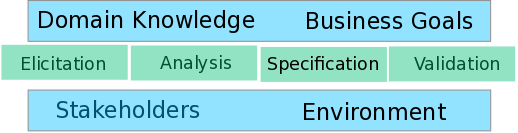
\includegraphics[width=0.8\linewidth]{img/requirements-engineering}
%Elicitation $\longrightarrow$ Analysis $\longrightarrow$ Specification $\longrightarrow$ Validation
%\end{centering}
%
\newpage
%\ifslides
%\else
%Zu klärende Fragen:\\[2ex]
%\fi
\begin{boxedminipage}{\linewidth}
\begin{itemize}
\item {\bfseries Wer} ist involviert?\\ 
(Benutzerprofil, Projektbeteiligte, Zuständigkeiten, Organigramm)
\item {\bfseries Wie} ist die gegenwärtige Situation?\\
  (Geschäftsprozesse, ev. Probleme, Schwachstellen)
\item {\bfseries Wann} muss das System lauffähig sein?\\
 (Termine, Meilensteine)
\item {\bfseries Wo} wird das System installiert?\\
  (HW/SW-Umgebung)
\item {\bfseries Warum} ist eine Neuentwicklung notwendig?\\
  (Zielsetzungen, Nutzen, Risiken)
\item {\bfseries Was} muss das System leisten?\\
 (Funktionalität, Mengengerüst)
\item {\bfseries Welche} Einschränkungen sind zu berücksichtigen?\\ 
(Programmiersprachen, Zuverlässigkeit, Antwortzeiten, Speicherbedarf etc.)
\end{itemize}
\end{boxedminipage}
\newslide
\vspace{0.5cm}

Ergebnisse:
\begin{itemize}
\item Anforderungsspezifikation (Requirements Specification)
\item Projektplan
\end{itemize}
InformationsSourcen:
\begin{itemize}
\item Interviews, Workshops
\item Fachliteratur, Zeitungen, Zeitschriften, Handb"ucher, Lexika
\item Dokumente, Formulare, Arbeitsanweisungen, Vorschriften
\item Internet
\end{itemize}
%\newpage
%
%--------------------------------------------------------------------------
%\ifslides
\newpage
%\fi
%\kopf
\section{Non-Functional Requirements}
%       \addcontentsline{toc}{subsection}{Nichtfunktionale Anforderungen}
Alle Anforderungen, die nicht im Systemmodell enthalten sind.\\[2ex]
Benutzerschnittstelle:
\begin{itemize}
\item An welche Benutzerkreise richtet sich das System?
\item Welcher Schulungsaufwand soll f\"ur die Benutzer vorgesehen werden?
\item Wieviel Gewicht soll auf die Verhinderung von Eingabefehlern
 gelegt werden?
\item Welche Ein- und Ausgabeger\"ate stehen zur Verf\"ugung und welches
  sind ihre Charakteristiken?
\end{itemize}
Dokumentation:
\begin{itemize}
\item Welche Dokumentationen m\"ussen erstellt werden?
\item Welche Leserkreise sollen damit angesprochen werden?
\end{itemize}
Hardware-Voraussetzungen:
\begin{itemize}
\item Auf welcher Hardware-Plattform wird das System ben\"utzt werden?
\item Welche Eigenschaften wird diese haben (Speicher, Disk, 
        Koprozessor etc.)?
\end{itemize}
Leistungsf\"ahigkeit:
\begin{itemize}
\item Gibt es irgendwelche Anforderungen bez\"uglich Rechengeschwindigkeit,
 Daten\-\"ubertragungsraten oder Antwortzeiten?
\item Gibt es bereits Einschr\"ankungen bezueglich Umfang oder Groesse der
 zu bearbeitenden Datens\"atze?
\end{itemize}
Fehlerbehandlung:
\begin{itemize}
\item Wie soll das System auf Eingabefehler reagieren?
\item Wie soll das System auf extreme Bedingungen reagieren?
\end{itemize}
\ifslides
\newpage
\fi
Programmschnittstellen:
\begin{itemize}
\item Sind Dateneingaben von anderen Programmsystemen vorzusehen?
\item Sind Datenausgaben an andere Programmsysteme vorzusehen?
\item Gibt es irgendwelche Einschr\"ankungen an das Ein- oder Ausgabeformat
resp. Medium?
\end{itemize}
\ifslides
\else
\newpage
\fi
Qualit\"atsanforderungen:
\begin{itemize}
\item Welche Anforderungen sind an die Zuverl\"assigkeit zu stellen?
\item Gibt es eine maximal zul\"assige Zeit zum Wiederaufstarten nach einem
eventuellen Systemabsturz?
\item Wie lange darf das System pro 24 Stunden ausfallen?
\item Muss das System auf andere Betriebssysteme und / oder 
Hardware-Plattformen portierbar sein?
\end{itemize}
\ifslides
\newpage
\fi
Modifikationen:
\begin{itemize}
\item Welche Teile des Systems sind m\"ogliche Kandidaten f\"ur 
sp\"atere Modifikationen?
\item Welche Modifikationen sind zu erwarten?
\end{itemize}
Physikalische Umgebung:
\begin{itemize}
\item Wo wird das realisierte System benutzt werden?
\item Sind dabei irgendwelche ungew\"ohnlichen Umweltbedingungen
 (Temperaturen, Feuchtigkeiten, Vibrationen, magnetische oder
 elektrische Felder etc.) zu erwarten?
\end{itemize}
Sicherheit:
\begin{itemize}
\item M\"ussen die Daten oder das System vor unberechtigtem
Zugriff gesch\"utzt werden?
\item Wie oft werden die Daten gesichert?
\end{itemize}
\ifslides
\newpage
\fi
Projektmanagement:
\begin{itemize}
\item Welche Mittel und Personen sind f\"ur den Entwurf, die Implementierung,
die Installation und den Unterhalt des Systems notwendig?
\item Welche Qualifikationen m\"ussen die Entwickler-Innen aufweisen?
\item Welche Termine sind einzuhalten?
\item Wie gross ist das Budget?
\item Wer ist verantwortlich f\"ur die Installation und Wartung?
\end{itemize}
\newpage
%--------------------------------------------------------------------------
%\section*{Systemanalyse}
%\subsection*{Nichtfunktionale Anforderungen}
%{\bfseries Beispiel:}
%\begin{verbatim}
%1. Benutzerschnittstelle
%  (a) Die Benutzer sind Projektierungsingenieure mit 
%      EDV-Kennt
%  (b) Die Einarbeitungszeit in die Systembedienung sol
%      mehr als 1 Tag beansp
%  (c) Die Benutzer sollen selbst in der Lage sein, sich 
%      Bedienung einzuar
%  (d) Das einzige Eingabegeraet ist die Tastatur, zur 
%      stehen ein Drucker und der Bildschirm zur Verfuegung.
%
%2. Hardware-Voraussetzungen
%  (a) Das System soll auf IBM-PC (oder kompatible) mit 256 kB
%      internem Speicher, einem 3 1/2-Zoll Floppy-Disk-Geraet 
%      und dem Betriebssystem DOS 3.3 betrieben werden.
%  (b) Das Programm soll auf einer 3 1/2 Zoll Diskette 
%      (DD = 720 kBytes) verteilt werden.
%  (c) Alle gaengigen Grafikkarten werden 
%      unterstuetzt (EGA,CGA,VGA).
%
%3. Leistungsfaehigkeit
%  (a) Es sollen  500 - 1000 verschiedene Normmotoren verwaltet 
%      werden koennen.
%  (b) Die Verarbeitungsgeschwindigkeit (Berechnung und Anzeige) 
%      soll mindestens 25 Motoren pro Minute betragen.
%
%4. Fehlerbehandlung
%  (a) Kritische Eingabefehler, die zum Beispiel zur Loeschung
%      von Datensaetzen fuehren koennten, sollen abgefangen werden.
%  (b) Falsche Eingaben sollten korrigiert werden koennen.
%
%5. Modifikationen:
%  (a) Das Programm soll in einer spaeteren Version auch fuer
%      Stromrichtersysteme verwendet werden koennen.
%  (b) Verbesserungen der Benutzerschnittstelle mit 
%      Mauseingabe und Fenstertechnik sind vorzusehen.
%\end{verbatim}
%\newpage
%--------------------------------------------------------------------------
%\section*{Systemanalyse}
% UI Mockups:
%  https://github.com/evolus/pencil
%  https://moqups.com/
%  https://balsamiq.com/
%  https://wireframe.cc/
%
\section{Software Requirements Specification (SRS)}

The Software Requirements Specification (SRS) establishes the basis for agreement between customers and
contractors or suppliers (in market-driven projects, these roles may be played by the marketing
and development divisions) on what the software
product is to do as well as what it is not expected
to do. It should also provide a realistic basis for estimating product costs, risks, and schedules.

Organizations can also use a SRS document as the basis for
developing effective verification and validation plans.

\newslide
Content: (Software Requirements Specification SRS IEEE Std 830, ISO/IEC/IEEE 29148)

\begin{tabbing}
{\bfseries\large Titel}\\
 Was, Wer, Wann, Wo\\
 Verteiler\\
 Inhaltsverzeichnis\\
 Zusammenfassung\\[1.5ex]
{\bfseries\large 1. Einleitung}{\em\ (Introduction)}\\
1.1 Zielsetzung {\em (Purpose)}\\
1.2 Geltungsbereich {\em (Scope)}\\
1.3 Definitionen und Begriffe {\em (Definitions and Acronyms)}\\
1.4 Referenzen {\em (References)}\\
1.5 \"Uberblick {\em (Overview)}\\[1.5ex]
\ifslides
\end{tabbing}
\newslide
\begin{tabbing}
\fi
{\bfseries\large 2. Allgemeine Beschreibung} {\em\ (General Description)}\\
2.1 Produktumfeld {\em (Product Perspective)}\\
2.2 Produktfunktionen {\em (Product Functions)}\\
2.3 Benutzercharakteristiken {\em (User Characteristics)}\\
2.4 Allgemeine Restriktionen {\em (General Constraints)}\\
2.5 Annahmen und Abh"angigkeiten {\em (Assumptions and Dependencies)}\\[1.5ex]
{\bfseries\large 3. Spezifische Anforderungen} {\em\ (Specific Requirements)}\\
Beschreibung der funktionalen und nicht-funktionalen Anforderungen
mit:\\
\ - UML-Diagrammen (Klassen- und Zustandsdiagramme)\\
\ - Datenflussdiagrammen, Aktivit\"ats-Spezifikationen, Datenkatalogen\\
\ - ER-Diagrammen (Datenbankmodell)\\
\ - Dateistrukturen, Protokolldefinitionen\\
\end{tabbing}
% https://github.com/rick4470/IEEE-SRS-Tempate#11-purpose
% https://github.com/jpeisenbarth/SRS-Tex
%
%Siehe auch: Volere Requirements Specification Template 
%\href{http://www.volere.co.uk/template.htm}{www.volere.co.uk/template.htm}

%product perspective: Business case, operational concept, external interfaces (Deployment Diagram)
%product functions: major functional capabilities, actors (Use Case Diagram)
%user characteristics: technical skills and capabilities of each user class
%constraints: regulatory policies; target platform, database, network software and protocols,
%  development standards requirements

%\ifslides 
%{\small
%Weitere Infos: \href{http://www.ktsi.ch/intranet/projekte/index.html}{www.ktsi.ch/intranet/projekte/index.html} (Username/Password: intra/testintra)
%}
%\else
%Weitere Infos: \href{http://www.ktsi.ch/intranet/projekte/index.html}{www.ktsi.ch/intranet/projekte/index.html} (Username/Password: intra/testintra)
%\newpage
%\fi
\newpage
Inhalt: (Pflichtenheft)
\begin{tabbing}
{\bfseries\large 1. Zielbestimmung}\\
1.1 Musskriterien \\
1.2 Wunschkriterien\\
1.3 Abgrenzungskriterien\\
{\bfseries\large 2. Produkteinsatz} \\
2.1 Anwendungsbereiche \\
2.2 Zielgruppen \\
2.3 Betriebsbedingungen\\
{\bfseries\large 3. Produktumgebung} \\
3.1 Software\\
3.2 Hardware\\
3.3 Orgware\\
3.4 Produktschnittstellen\\
\newslide
{\bfseries\large 4. Produktfunktionen} \\
4.1 Funktion 1\\
4.2 Funktion 2\\
\ldots\\

{\bfseries\large 5. Produktdaten} \\
5.1 Daten 1\\
\ldots\\

{\bfseries\large 6. Produktleistungen} \\
{\bfseries\large 7. Benutzungsoberfläche} \\
{\bfseries\large 8. Qualitätszielbestimmung} \\
{\bfseries\large 9. Globale Testszenarien/Testfälle} \\
{\bfseries\large 10. Entwicklungsumgebung} \\
{\bfseries\large 11. Ergänzungen} \\
\end{tabbing}
(Source: Helmut Balzert, Lehrbuch der Software-Technik)

%------------------------------------------------------------------------
%\section*{Systemanalyse}
\subsection{Review}
%       \addcontentsline{toc}{subsection}{Beurteilung (Review)}
%\begin{tabbing}
%Datum:\\[2ex]
%Ausf\"uhrende:\\[2ex]
%Thema:\\[2ex]
%\end{tabbing}
\begin{tabular}{llp{5cm}c}
 \hline
% &  &  &  \\
{\large\bfseries Form} & \\
        & \underline{Sprache} & \\
        &  Ausdruck, Formulierungen    & klar, verst\"andlich, eindeutig\\
        &   Grammatik, Rechtschreibung  & korrekt\\[2ex]
        & \underline{Struktur} & \\
        &    Aufbau, Gliederung         & logisch, \"ubersichtlich \\[2ex]
        & \underline{Darstellung} & \\
         &   Layout       & einheitlich, zweckm\"assig \\
         &   Zeichnungen, Bilder & beschriftet, normgerecht\\[2ex]
\hline
\ifslides
\end{tabular}
\newpage
\begin{tabular}{llp{5cm}c}
 \hline
\fi
% &  &  & \\
{\large\bfseries Inhalt} & \\
       & \underline{L\"osungsansatz} & \\
       &   Idee & origin\"ar, innovativ \\
       &  Praktikabilit\"at & \\[2ex]
       & \underline{Vollst\"andigkeit}  &  \\ 
       &   Aufgabenstellung, Thematik & verstanden \\
       &   Anforderungen, Projektziele & spezifiziert \\
       &   Funktionalit\"at & erfasst \\[2ex]
       & \underline{Korrektheit}        & \\ 
       &   Anforderungen, Ziele, Modelle & konsistent, widerspruchsfrei\\[2ex]
\hline
\ifslides
\end{tabular}
\newpage
%
\begin{tabular}{llp{5cm}c}
 \hline
\fi
%  &  & & \\
  Entscheid & \\
       &\usebox{\rk} akzeptiert\\
       &\usebox{\rk} akzeptiert mit kleinen \"Anderungen\\
       &\usebox{\rk} abgelehnt\\
       &\usebox{\rk} Projektabbruch\\
\end{tabular}
\newpage
\subsection{Exercise}
Untersuchen und bewerten Sie eine Anforderungsspezifikation. 
Verwenden Sie dabei die folgenden IEEE-Kriterien:
\begin{itemize}
\item vollständig (complete)
\item korrekt (correct)
\item konsistent (consistent)
\item prüfbar (verifiable)
\item eindeutig (unambigous)
\item verfolgbar (traceable)
\item priorisiert (ranked)
\item machbar (feasible)
\end{itemize}
\newslide

%It is unreasonable to expect that business stakeholders can
%articulate a set of complete fully-developed consistent requirements
%(Alan Mc Sweeney, 2016)

%
%Vorschläge:
%\begin{itemize}
%\item Personal Investment Management System (PIMS):
%Management of the investment of a single user (portfolio, security, transaction)

%\href{http://www.cse.iitk.ac.in/JaloteSEbook/CaseStudies/CaseStudy2/SRS.pdf}
%  {www.cse.iitk.ac.in/JaloteSEbook/CaseStudies/CaseStudy2/SRS.pdf}
%
%\item NetBeans Plugin for ER-Diagrams
%\href{http://wiki.netbeans.info/wiki/attach/ERDModuleRequirements/SRS%20final%20document.doc}
%{wiki.netbeans.info/wiki/attach/ERDModuleRequirements/SRS\%20final\%20document.doc}
%
%\item University Student Registration
%
%\href{http://www.nyu.edu/classes/jcf/g22.2440-001/handouts/Assignment1SampleSolution.pdf}
%{www.nyu.edu/classes/jcf/g22.2440-001/handouts/Assignment1SampleSolution.pdf}
%\item Space-Fractions: an interactive game to improve fraction-solving skills for sixth-grade students

%\href{http://users.snip.net/~gbooker/ISYS425/SRSSample.pdf}
%          {users.snip.net/~gbooker/ISYS425/SRSSample.pdf}
%
%\item Cafeteria-Ordering-System (COS)
%
%\href{http://www.tol.oulu.fi/kurssit/otekniikka/papers/COS_SRS.pdf}
%  {www.tol.oulu.fi/kurssit/otekniikka/papers/COS\_SRS.pdf}

%\item Brettspiele
%
%\href{http://www.stefan-baur.de/downloads/Lastenheft.pdf}
%   {www.stefan-baur.de/downloads/Lastenheft.pdf}

%\item PersonalShoppingAssistant (PSA)
%
%\href{http://www.informatik.uni-bremen.de/st/Lehre/swp0708/abgabe2.html}
%{www.informatik.uni-bremen.de/st/Lehre/swp0708/abgabe2.html}
%\end{itemize}
% Allg: http://www.informatik.uni-bremen.de/st/Lehre/
%------------------------------------------------------------------------
% 

% -----------------------------------------------------------------------
\chapter{Object Oriented Programming}
%-----------------------------------------------------------------------
\section{Introduction}
Object-oriented programming is a programming paradigm based on the
concept of \emph{objects}, which can contain data, in the form of
fields (attributes or properties), and code, in the form of procedures
(methods).\\
The key concepts in OOP are:
\begin{itemize}
\item Abstraction (objects, classes)
\item Data Encapsulation
\item Inheritance
\item Polymorphism
\end{itemize}
The following chapter will give a brief overview of the key concepts
in object oriented programming. This is of course not a course about
object oriented programming. But it makes perfectly sense to understand
the key concepts as they are also used in several areas of software
engineering.

\section{Languages}
There are many object oriented programming languages available.
Each language has its advantages and disadvantages. The most popular
languages are:
\begin{itemize}
\item C++
\item Java
\item .Net
\item Python
\item ...and many more!
\end{itemize}

\section{Abstraction}
Abstraction means using simple things to represent complexity.
We all know how to turn the TV on, but we do not need to know how
it works in order to enjoy it. In OOP, abstraction means simple
things like objects, classes, and variables represent more complex
underlying code and data. This is important because it lets avoid
repeating the same work multiple times.

\begin{lstlisting}
public class TV {
  private Color color;
  private int size;
  public void turnOn(){ // some complex code }
  public void turnOff(){ // some complex code }
  public void changeChannel(){ // some complex code }
}

TV tv1 = new TV();
TV tv2 = new TV();
\end{lstlisting}
TV is the class definition. \verb|tv1| and \verb|tv2| are the
objects. They both have their own color and size.

\section{Data Encapsulation}
This is the practice of keeping fields within a class private,
then providing access to them via public methods. It's a protective
barrier that keeps the data and code safe within the class itself.
This way, we can re-use objects like code components or variables
without allowing open access to the data system-wide.

\begin{lstlisting}
public class Circle {
  private double radius;
  public void setRadius(double radius) {this.radius = radius;}
  public void getRadius() {return radius;}
}

Circle circle = new Circle();
circle.setRadius(10); // correct way
circle.radius = 10; // compilation error, radius is private
\end{lstlisting}

\section{Inheritance}
This is a special feature of Object Oriented Programming.
It lets programmers create new classes that share some of the
attributes of existing classes. This lets us build on previous work
without reinventing the wheel.

\begin{lstlisting}
public class Doctor {
  protected String name;
  public void doctorDetails() { // do some stuff }
}

public class Surgeon extends Doctor {
  public void surgeonDetails() { // do some stuff }
}

Surgeon jamesMiller = new Surgeon();
jamesMiller.surgeonDetails();
jamesMiller.doctorDetails();
\end{lstlisting}

The object \verb|jamesMiller| is a doctor and a surgeon.

\section{Polymorphism}
This OOP concept lets programmers use the same word to mean
different things in different contexts. One form of polymorphism
is method overloading. That's when different meanings are implied
by the code itself. The other form is method overriding. That's when
the different meanings are implied by the values of the supplied
variables.

\begin{lstlisting}
public abstract class DBConnection {
  public abstract void connect();
};

public class OracleConnection extends DBConnection {
  public void connect() { // connect to oracle db }
};

public class SQLServerConnection extends DBConnection {
  public void connect() { // connect to sql server db }
};

DBConnection connection1 = new OracleConnection();
DBConnection connection2 = new SQLServerConnection();
connection1.connect();
connection2.connect();
\end{lstlisting}

Both objects, \verb|connection1| and \verb|connection2| are of
type \verb|DBConnection|. During runtime, the \verb|connection1| object
will point to a \verb|OracleConnection| object, the
\verb|connection2| object will point to a \verb|SQLServerConnection| object.
When calling the \verb|connect| method o both objects, a different method
will be called.

\section{Exercises}
\begin{enumerate}
\item Write a class called \verb|Util|. This class should contain a method
\verb|createSampleDNA| which will create a sample DNA sequence of
a given length.\\
The program should be callable from the command line. One parameter
could be provided, which specifies the length of the sequence. If
no parameter is provided, the default length is 100.
\item Extend your \verb|Util| class with a method which counts the
number of A, G, C and T in a given sequence. The sequence will also
be provided as parameter.
\item Implement the data loader component. Create a project in your
preferred development environment and create on class \verb|Loader|.
This class should fulfill the following steps:
\begin{itemize}
\item The program should be called with a properties file as parameter.
This file will contain information like db location, username and password.
\item The program will read the data file line by line
\item The program will insert the data into the database
\item Please ensure that the program is running with an acceptable performance and resource consumption
\end{itemize}
\item If the data is loaded, please try to answer the following questions by
using SQL statements:
\begin{itemize}
\item How many gene information entries are available?
\item How many genes have the type \emph{protein-coding}?
\item How many genes have the type \emph{protein-coding} and are
related to the specie \emph{Human}?
\end{itemize}
\end{enumerate}

\subsection{SQL Help}
\begin{lstlisting}
drop database if exists XZY;

create database XYZ;

use XZY;

create table TTT (
  column1 varchar(256),
  column2 int,
  ...,
  PRIMARY KEY(column1),
  FOREIGN KEY(column2) REFERENCES TABLE_X(column_x)
);

CREATE USER 'dataloader'@'localhost' IDENTIFIED BY 'password';
GRANT ALL PRIVILEGES on XZY.* TO 'dataloader'@'localhost';
FLUSH PRIVILEGES;
\end{lstlisting}

%--------------------------------------------------------------------------
\chapter{System Analysis and Design using UML}
%
The {\em Unified Modeling Language} (UML) is a general-purpose, developmental,
modeling language in the field of software engineering that is
intended to provide a standard way to visualize the design of a system:
\begin{quote}
The Unified Modeling Language (TM)
 -- UML -- is OMG's most-used specification, and
the way the world models not only application structure, behavior, and
architecture, but also business process and data structure.
\end{quote}

Likewise building plans are created in many other areas, e.g.
architects, machine design, electronic circuits, plans are
also needed for the design and implementation of software
systems.

%Analog zu den Bauplänen, die für Architekten, Maschinenkonstrukteure
%und Elektroniker unabdingbar und selbstverständlich sind,
%hat sie den Anspruch (oder vielmehr das Ziel) solche
%Systeme generell, vollständig und eindeutig zu beschreiben.

\ifslides
\newslide
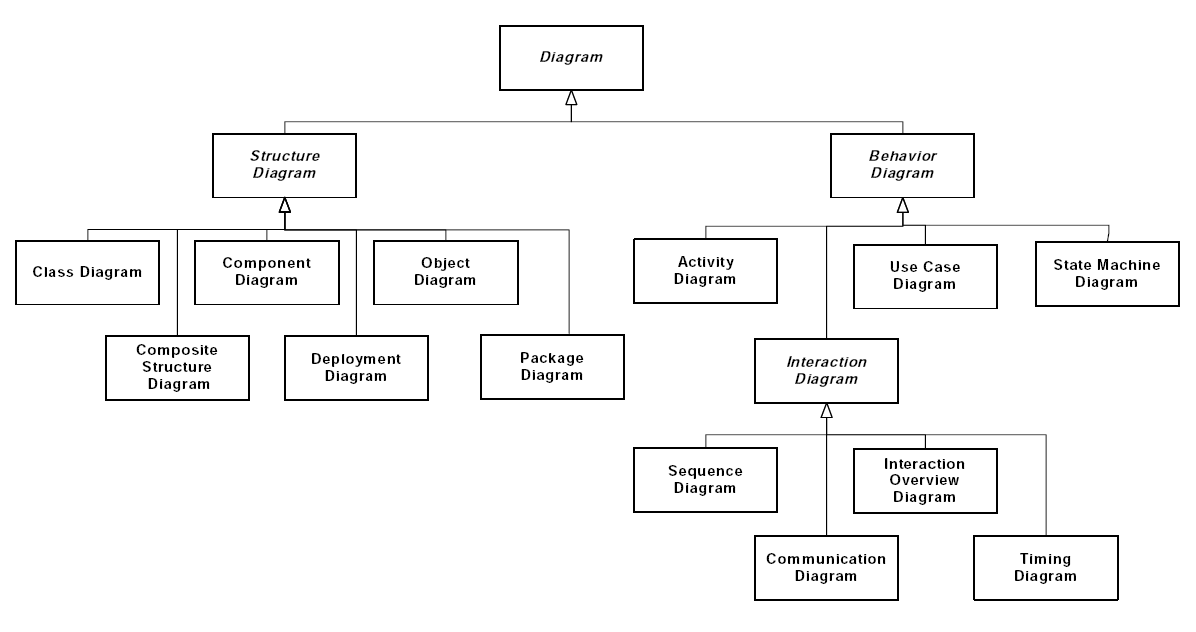
\includegraphics[width=\linewidth]{uml/img/uml-diagrams}
\newslide
\else
UML contains diagrams which could be used for all
areas in the design of a software system.
%Die UML umfasst spezielle Diagramme für
%die Darstellung der verschiedenen Aspekte
%eines Softwaresystems:

\begin{figure}[H]
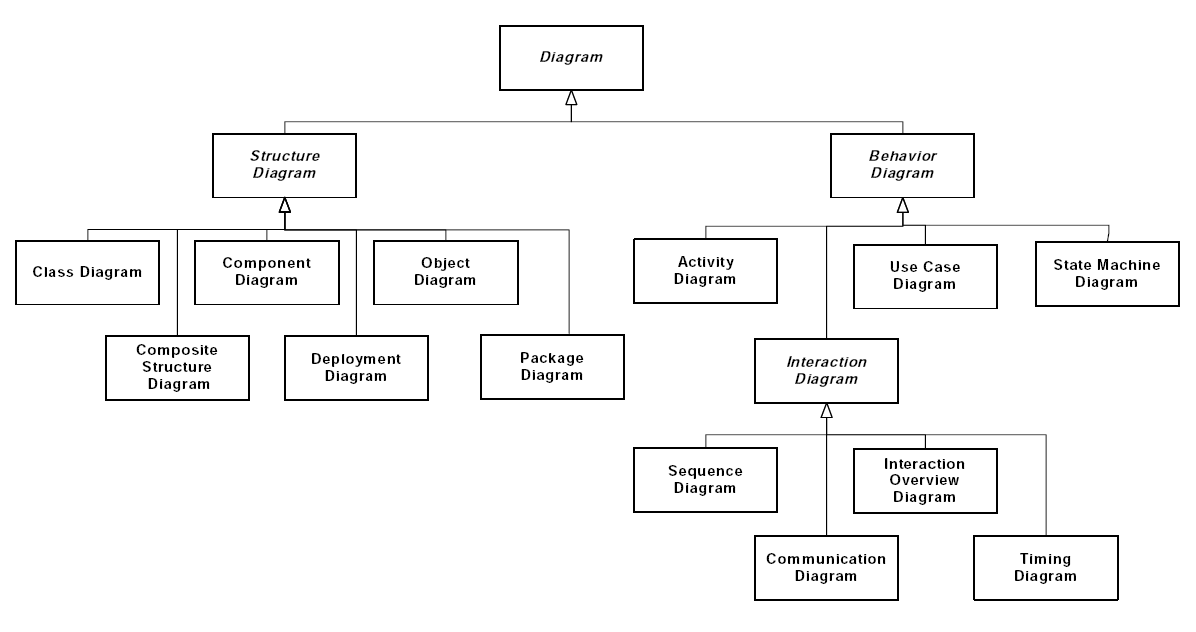
\includegraphics[width=\linewidth]{uml/img/uml-diagrams}
\caption{The Diagrams of UML 2 (Source: OMG)}
\end{figure}
\fi

Für den vereinfachten Austausch der UML-Modelle zwischen
Entwicklungswerkzeugen verschiedener Hersteller wird von OMG auch das
Datenformat {\em XML Metadata Interchange (XMI)} definiert.

%Dazu wird in der Regel ein
% formales Modell erstellt, das die essentiellen Aspekte
%des Systems beschreibt resp. spezifiziert.
\newpage
The current UML standards call for 13 different types of diagrams:
\begin{description}
\item[Structural UML diagrams:] Structure diagrams emphasize the things that
must be present in the system being modeled:
  \begin{description}
  \item[Class Diagram:] Class diagrams are the backbone of almost
  every object-oriented method, including UML. They describe the
  static structure of a system.
  \item[Package Diagram:] Package diagrams are a subset of class
  diagrams, but developers sometimes treat them as a separate
  technique. Package diagrams organize elements of a system into
  related groups to minimize dependencies between packages.
  \item[Component Diagram:] Component diagrams describe the
  organization of physical software components, including
  source code, run-time (binary) code, and executables.
  \item[Deployment Diagram:] Deployment diagrams depict
  the physical resources in a system, including nodes,
  components, and connections.
  \end{description}
\item[Behavioral UML diagrams:] Behavior diagrams emphasize what must
happen in the system being modeled:
  \begin{description}
  \item[Use-Case Diagram:] Use case diagrams model the functionality
  of a system using actors and use cases.
  \item[State-Transition Diagram:] State-Transition diagrams,
  now known as state machine diagrams and state diagrams describe
  the dynamic behavior of a system in response to external stimuli.
  State diagrams are especially useful in modeling reactive objects
  whose states are triggered by specific events.
  \item[Activity Diagram:] Activity diagrams illustrate the dynamic
  nature of a system by modeling the flow of control from activity
  to activity. An activity represents an operation on some class in
  the system that results in a change in the state of the system.
  Typically, activity diagrams are used to model workflow or business
  processes and internal operation.
  \item[Interaction diagram:] Interaction diagrams describe interactions
  among classes in terms
  of an exchange of messages over time.
  \item[Timing Diagram:] A timing diagram is a type of behavioral or
  interaction UML diagram that focuses on processes that take place
  during a specific period of time. They're a special instance of a
  sequence diagram, except time is shown to increase from left to right
  instead of top down.
  \end{description}
\end{description}
\newpage
%--------------------------------------------------------------------------
%\subsection{UML-Diagramme}
\section{Class Diagram}
The class diagram is the main building block of object-oriented
modeling. It is used for general conceptual modeling of the
structure of the application, and for detailed modeling translating
the models into programming code. Class diagrams can also be used for
data modeling. The classes in a class diagram represent both the
main elements, interactions in the application, and the classes to be
programmed.

\ifslides
\newpage
\paragraph{Class}\\[2ex]
\begin{minipage}[c]{0.45\linewidth}
\else
\paragraph{Class}\mbox{} \\
\begin{minipage}[c]{0.5\linewidth}
\fi
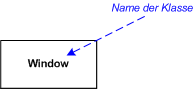
\includegraphics[width=\linewidth]{uml/img/Class-1}\\

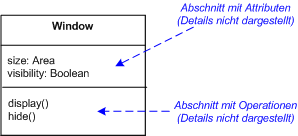
\includegraphics[width=\linewidth]{uml/img/Class-2}\\

%\includegraphics[width=3cm]{uml/img/Class-3}\\
%
{\footnotesize Source: wikipedia}
\end{minipage}
\hfill
\begin{minipage}[c]{0.45\linewidth}
A class contains a name, attributes and methods. Attributes and
methods could be hidden if they do not cover an important part in
the system design.
\end{minipage}
%
\paragraph{Interface}\mbox{} \\
\begin{minipage}[c]{0.28\linewidth}
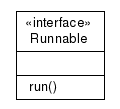
\includegraphics[width=3cm]{uml/img/interface}
\end{minipage}
\begin{minipage}[c]{0.7\linewidth}

Interface are similar to abstract classes.
It is a collection of abstract methods.
A class implements an interface, thereby inheriting
the abstract methods of the interface.
Along with abstract methods, an interface may also
contain constants, default methods, static methods,
and nested types.
\end{minipage}
%
\ifslides
\newpage
\fi
\paragraph{Abstract class}\mbox{} \\
\begin{minipage}[c]{0.28\linewidth}
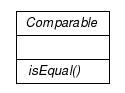
\includegraphics[width=3cm]{uml/img/abstract}
\end{minipage}
\begin{minipage}[c]{0.7\linewidth}
An abstract class is a class that is declared abstract. It
may or may not include abstract methods.
Abstract classes cannot be instantiated, but they can be subclassed.
\end{minipage}
%
\newpage
%
\paragraph{Attributes and Methods}\mbox{} \\
\begin{minipage}{0.3\linewidth}
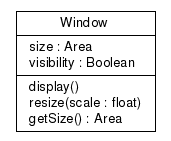
\includegraphics[width=\linewidth]{uml/img/window}
\end{minipage}
\hfill
\begin{minipage}{0.65\linewidth}

An \structure{attribute} is an individual thing that differentiate one object from
another and determine the appearance, state, or other qualities of that object.
Each object for a class has the given set of attributes with
own values.

A \structure{class attribute} is an attribute which exists only once
for all objects. All objects of a given class share the same attribute.
Class attributes are underlined.

A \structure{method} is a set of statements to perform an operation.
Sometimes, a method is also called member function.

A \structure{class method} is an operation which does not depend on any object
of that class. This method could also be called if there is no object of the
class (e.g. utility method), therefore a class method could not access any
attributes (expect class attributes).
\end{minipage}

%Eine abstrakte Operation ist eine Operation, f\"ur die nur eine Signatur,
%jedoch keine Anweisungsfolge definiert ist, d.h. die Operation ist definiert,
%aber noch nicht implementiert. Sie wird in einer abgeleiteten Klasse
%implementiert. Abstrakte Operationen werden \"ublicherweise durch
%Kursivschrift gekennzeichnet.
\ifslides
\newpage
\fi
%
\paragraph{Visibility}\mbox{} \\
\begin{minipage}[c]{0.4\linewidth}
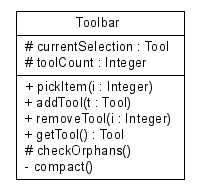
\includegraphics[width=0.85\linewidth]{uml/img/visibility}
\end{minipage}
\begin{minipage}[c]{0.58\linewidth}
There are 3 different types of visibility for attributes and methods:

\begin{description}
\item [-- Private] only visible within the class

\item [\# Protected] visible in the class itself and all inherited classes

\item [+ Public] visible from everywhere, no protection.
\end{description}
\end{minipage}

%\ifslides
\newpage
%\fi
\paragraph{Inheritance} (generalization)\\[2ex]
\begin{minipage}[c]{0.5\linewidth}
\ifslides
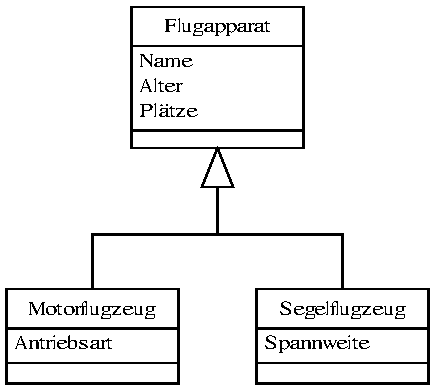
\includegraphics[width=\linewidth]{uml/img/Vererbung}
\else
\includegraphics[width=\linewidth]{uml/img/Vererbung}
\fi
\end{minipage}
\begin{minipage}[c]{0.45\linewidth}

In object-oriented programming, inheritance is the mechanism of basing an
class upon another class, retaining similar implementation. Also defined as
deriving new classes (sub classes) from existing ones (super class)
and forming them into a hierarchy of classes. Aan object created through
inheritance acquires all the properties and behaviors of the parent
object (except: constructors, and some other language specific constructs).
Inheritance allows programmers to create classes
that are built upon existing classes, to specify a new implementation while
maintaining the same behaviors (realizing an interface), to reuse code and to
independently extend original software via public classes and interfaces.
\end{minipage}
%
\newpage
\paragraph{Association}\mbox{} \\
\begin{minipage}[c]{0.28\linewidth}
\ifslides
\includegraphics[width=3.2cm]{uml/img/Assoziation}
\else
\includegraphics[width=3.7cm]{uml/img/Assoziation}
\fi
\end{minipage}
\begin{minipage}[c]{0.7\linewidth}
An \structure{association} defines a relationship between classes of
objects that allows one object instance to cause another to perform an action
on its behalf. This relationship is structural, because it specifies that
objects of one kind are connected to objects of another and does not
represent behaviour.
\end{minipage}
%
\ifslides
\newpage
\fi
\paragraph{Aggregation}\mbox{} \\
\begin{minipage}[c]{0.28\linewidth}
\includegraphics[width=3cm]{uml/img/Aggregation}
\end{minipage}
\begin{minipage}[c]{0.7\linewidth}
Inheritance is a \verb|"|is-a\verb|"| relation (e.g. a dog (sub class) is a animal
(super class)). An \structure{aggregation} contains a whole/part
relationship (\verb|"|has-a\verb|"|). A synonym for this is \verb|"|part-of\verb|"|.
\end{minipage}
%
\ifslides
\newpage
\fi
\paragraph{Composition}\mbox{} \\
\begin{minipage}[c]{0.28\linewidth}
\includegraphics[width=3cm]{uml/img/Komposition}
\end{minipage}
\begin{minipage}[c]{0.7\linewidth}
A \structure{composition} is a restricted form of Aggregation in which two
entities are highly dependent on each other. When there is a composition
between two entities, the composed object cannot exist without the other entity.
\end{minipage}
%
\ifslides
\newpage
\fi
\paragraph{Comment} (note)\\[2ex]
\begin{minipage}[c]{0.3\linewidth}
\ifslides
\includegraphics[width=3.5cm]{uml/img/Kommentar1}
\else
\includegraphics[width=4.3cm]{uml/img/Kommentar1}
\fi
\end{minipage}
\begin{minipage}[c]{0.69\linewidth}
Comments could be added for additional clarification or description.
\end{minipage}
%
\newpage
\ifslides
\paragraph{Beispiel}\ \\
\includegraphics[width=0.9\linewidth]{uml/img/Beobachter}
\else
\paragraph{Beispiel}
Ein Objekt soll in der Lage sein, andere Objekte zu benachrichtigen,
ohne Annahmen dar\"uber zu treffen, wer die anderen Objekte sind.
Mit anderen Worten: gesucht ist eine Struktur mit
 möglichst lose gekoppelten Objekten.
Die L\"osung dieses Problems ist unter dem Begriff
Beobachter (Observer) bekannt.
%
\begin{figure}[H]
\begin{center}
\includegraphics[width=\linewidth]{uml/img/Beobachter}
\caption{Entwurfsmuster Beobachter}
\end{center}
\end{figure}
\fi
%
%\begin{center}
%\ifslides
%\includegraphics[width=0.4\linewidth]{uml/xfig/uml-classdiagram}
%\else
%\includegraphics[width=0.7\linewidth]{uml/xfig/uml-classdiagram}
%\fi
%\end{center}
\ifslides
\newpage
\fi
\underline{Vorgehen}
\begin{enumerate}
\item Klassen und Beziehungen identifizieren,
\item die relevanten Attribute und Methoden hinzuf\"ugen,
\item generalisieren durch Vererbung,
\item die Klassen in Kategorien (Module) gruppieren
\end{enumerate}
%--------------------------------------------------------------------------
\newpage
\subsection{The Creation of Class Diagrams}
\underline{1. Schritt: Identifizieren von Klassen und deren Beziehungen}\\[2ex]
Ausgangspunkt ist den meisten F\"allen eine verbale Beschreibung des
Problembereichs im Vokabular des Anwenders. Eine g\"angige, wenn
auch zum Teil kritisierte, Methode
zur Identifizierung der Klassen (und Objekte) basiert auf einer Textanalyse,
bei der die Substantive als m\"ogliche Kandidaten dienen:\\[2ex]
\begin{tabularx}{\linewidth}{l|X}
Personen, Rollen & Lieferant, Kunde, Mitarbeiter, Student, Dozent \\
Dinge, Ger\"ate  & Beh\"alter, Tank, Regler, Pumpe, Zeitgeber, Schalter,
            Messger\"at, Sensor, Filter, Anzeige\\
Abstraktionen & Stack, Array, Tabelle, Sequenz, Menge, Figur, Dreieck, Linie,
    Datei, Baustein, Element\\
%%\item[Orte]
Beschreibungen, Dokumente & Rezeptur, Produkt, Konto\\
Ereignisse, Vorg\"ange & Prozess, Simulation, Steuerung, Nachricht\\
Interaktionen& Bestellung, Kaufvertrag, Buchung, Reservation,
Anmeldung, Auftrag
%%\item[Externe Systeme]
%%\item[Organisationseinheiten]
\end{tabularx}

In der Regel findet man in einer ersten Analyse des Problembereichs
mehr Klassen, als man wirklich ben\"otigt. Auf weiter zu verwendende Klassen
m\"ussen die folgenden Aussagen zutreffen:
\begin{enumerate}
\item Ihr Name ist eindeutig, d.h. kein Synonym einer bereits
 ausgew\"ahlten Klasse.
\item Sie enth\"alt Informationen (Attribute), die innerhalb
  des Systems gespeichert werden sollen.
\item Sie stellt system-relevante Operationen zur Verf\"ugung (mehr als
   nur Setzen und Abfragen).
\end{enumerate}
Beziehungen zwischen den Objekten entsprechen physischen oder
logischen Verkn\"upfungen mit zugeh\"origen Kardinalit\"aten
analog den Relationen zwischen Entit\"aten:
\begin{itemize}
\item Assoziation: semantische Verkn\"upfung
\item Aggregation: ``hat-ein''-Verkn\"upfung
\item Verwendung: Nutzungs-Verkn\"upfung
\item Vererbung: ``ist-ein''-Verkn\"upfung
\end{itemize}
\newpage
%--------------------------------------------------------------------------
%{\bfseries Beispiel:} Es soll ein einfaches
%Zeichnungsprogramm entwickelt werden, mit welchem der Anwender
%verschiedene Figuren (Linien, Rechtecke) mit dem Mauszeiger
%erzeugen und in einer
%Zeichenfl\"ache darstellen kann.
%Eine Reihe in senkrechter Kolonne angeordneter und
%gegenseitig sich ausschliessender
%Kontrollkn\"opfe, die sich am rechten (oder linken) Rand der
%Zeichenfl\"ache befindet, erlaubt die Auswahl des zu zeichnenden Figurentyps.
%Mit einer weiteren solchen Reihe kann die Farbe gew\"ahlt werden.
%Schliesslich gibt es noch Druckkn\"opfe zum L\"oschen oder Verlassen des
%Programms.
%\newpage
%--------------------------------------------------------------------------
%\subsection*{Objektorientierte Analyse (Object-Oriented Analysis)}
{\bfseries Beispiel:} Klassendiagramm eines bekannten Spiels:\\[1.5ex]
%%
\begin{center}
\ifslides
\includegraphics[width=0.77\linewidth]{uml/img/monopoly}
\else
\includegraphics[width=0.9\linewidth]{uml/img/monopoly}
\fi
\end{center}
\ifslides
\else
{\footnotesize Source: Craig Larman}\\[2ex]
\fi
%--------------------------------------------------------------------------
%\subsection*{Klassendiagramm}
\underline{2. Schritt: Hinzuf\"ugen der relevanten Attribute und Methoden}
\begin{itemize}
\item Attribute sind die Eigenschaften der Objekte:
\begin{enumerate}
\item Wie wird das Objekt allgemein beschrieben?
\item Wie wird das Objekt im Problembereich beschrieben?
\item Können zusammengehörende Attribute zu einer Gruppe
  zusammengefasst werden?
 (Bsp: Vorname, Nachname, Anrede ergibt Name)
\end{enumerate}
\item Methoden sind die Dienste, die ein Objekt bereitstellt:
\begin{enumerate}
\item Berechnungen
\item \"Uberwachung
\item Kommunikation
\end{enumerate}
aus Gründen der \"Ubersichtlichkeit sollen nur explizite und
keine impliziten Methoden im Objektmodell dargestellt werden.
Implizite Methoden sind: Konstruktorfunktionen, Zugriffsfunktionen zu den
  Attributen, Verbindungsfunktionen zum Setzen und L\"osen von Verbindungen.
\end{itemize}
\newpage
\underline{3. Schritt: Generalisieren durch Vererbung}\\[2ex]
Durch eine Vererbungsstruktur werden Klassen
die
\begin{itemize}
\item Spezialfälle einer andern Klasse sind oder
\item gemeinsame Attribute mit andern Klassen haben
\end{itemize}
in einer gemeinsamen Basisklasse zusammengefasst.\\[3ex]
\underline{4. Schritt: Gruppierung der Klassen in Kategorien}
\begin{itemize}
\item Jede Klasse ist Teil genau einer Kategorie.
\item Die Kopplung zwischen Klassen unterschiedlicher Kategorien ist minimal.
\end{itemize}
\ifslides
\newpage
\fi
%--------------------------------------------------------------------------
\section{Interaction Diagrams}
An \structure{interaction diagram} visualizes the interactions between
objects.

One interaction diagram normally demonstrates the behavior of one
single use case. The diagram shows a number of objects as well as
all messages which are exchanged between these objects.

There are two types of interaction diagrams:
sequence diagram and collaboration diagram

%
\paragraph{Sequence diagram}\mbox{} \\
A \structure{sequence diagram} shows object interactions arranged in time sequence.
It depicts the objects and classes involved in the scenario and the sequence
of messages exchanged between the objects needed to carry out the
functionality of the scenario.

A sequence diagram shows, as parallel vertical lines (lifelines),
different processes or objects that live simultaneously, and, as
horizontal arrows, the messages exchanged between them, in the order in
which they occur. This allows the specification of simple runtime scenarios
in a graphical manner.

%Um zu zeigen, dass ein Objekt aktiv ist, kann man einen
%\emph{Aktivierungskasten} (engl.
%activitation box) hinzuf\"ugen. Man kann
%Aktivierungsk\"asten weglassen, wodurch die Diagramme
%einfacher zu zeichnen, jedoch auch schwieriger zu verstehen werden.

%Zwei Anteile der Steuerinformationen k\"onnen besonders n\"utzlich sein.
%
%Erstens kann eine \emph{Einschr\"ankung} angeben, wann
%eine Nachricht gesendet wird. Die Nachricht
%wird nur gesendet, wenn die Einschr\"ankung wahr ist.
%
%Die zweite n\"utzliche Steuermarkierung ist die Iterationsmarkierung.
%Sie zeigt an, dass eine
%Nachricht mehrfach an viele Empf\"angerobjekte gesendet wird. Woraus
%sich die Iteration ergibt,
%kann man in eckigen Klammern darstellen
%(wie z.B. *[f\"ur alle
%Auftragspositionen]).

%Das Löschen eines Objekts wird mit einem grossen \textbf{X} markiert.
%\ifslides
%\else
%
%Auftragsbearbeitung als Sequenzdiagramm.
%\fi
%
\begin{figure}[H]
\begin{center}
\ifslides
\includegraphics[width=0.7\linewidth]{uml/img/uml-sequence-diagram}
\else
\includegraphics[width=\linewidth]{uml/img/uml-sequence-diagram}
\fi
\caption{Sequenzdiagramm}
\label{SEQ}
\end{center}
\end{figure}
\ifslides
\begin{center}
\includegraphics[width=0.75\linewidth]{uml/img/dnsquery}
\end{center}
\else
\begin{figure}[H]
\begin{center}
\includegraphics[width=\linewidth]{uml/img/dnsquery}
\caption{Sequenzdiagramm einer DNS-Abfrage (Source: Craig Larmann)}
%\label{SEQ}
\end{center}
\end{figure}
\fi
%
\paragraph{Collaboration diagram}\mbox{} \\
A \structure{collaboration diagram} models the interactions between objects
or parts in terms of sequenced messages. Collaboration diagrams represent
a combination of information taken from Class, Sequence, and Use Case
Diagrams describing both the static structure and dynamic behavior of a system.

However, communication diagrams use the free-form arrangement of objects
and links as used in Object diagrams. In order to maintain the ordering of
messages in such a free-form diagram, messages are labeled with a
chronological number and placed near the link the message is sent over.
Reading a communication diagram involves starting at message 1.0, and
following the messages from object to object.

Communication diagrams show a lot of the same information as sequence
diagrams, but because of how the information is presented, some of it
is easier to find in one diagram than the other. Communication diagrams
show which elements each one interacts with better, but sequence
diagrams show the order in which the interactions take place more clearly.

\ifslides
\includegraphics[width=0.9\linewidth]{uml/img/uml-collaboration-diagram}
\else
\paragraph{Beispiel}
%Auftragsbestellung
%
\begin{figure}[H]
\begin{center}
\includegraphics[width=\linewidth]{uml/img/uml-collaboration-diagram}
\caption{Kollaborationsdiagramm}
\label{fig:KOL1}
\end{center}
\end{figure}
%
\fi
%%
\ifslides
\newpage
\fi
\underline{Vorgehen}
\begin{enumerate}
\item Szenarien entwerfen
\item Ereignisse und betroffene Objekte identifizieren
\item Ereignispfad skizzieren
\end{enumerate}
%\newpage
\ifslides
\newpage
\fi
%--------------------------------------------------------------------------
\section{State Transition Diagram}
%%% (Sequence und State-Transition-Diagram)}
State transition diagrams are used to give an abstract description of the behavior of a
system. This behavior is analyzed and represented by a series of events that
can occur in one or more possible states. Hereby each diagram usually
represents objects of a single class and track the different states of its
objects through the system. An object is always in one (and only one) state.
If a event occurs, the state may change.

%
\ifslides
\begin{center}
\includegraphics[width=0.8\linewidth]{uml/img/uml-state-diagram}
\end{center}
\else
\newpage
\paragraph{Beispiel}\ \\[2ex]
The following diagram shows the different states for an order (online shop).
\begin{figure}[H]
\begin{center}
\includegraphics[width=\linewidth]{uml/img/uml-state-diagram}
\caption{Zustandsdiagramm}
\end{center}
\end{figure}
\fi
%
\paragraph{Anfangszustand}\ \\[2ex]
\begin{minipage}[c]{0.1\linewidth}
\includegraphics[width=0.8cm]{uml/img/Anfangszustand}
\end{minipage}
\begin{minipage}[c]{0.89\linewidth}
Jeder Zustandsautomat muss einen Anfangszustand besitzen.
Es handelt sich um einen Pseudozustand, der durch eine
Transition mit einem echten Zustand verbunden ist.
\end{minipage}
%
\paragraph{Endzustand}\ \\[2ex]
\begin{minipage}[c]{0.1\linewidth}
\includegraphics[width=1cm]{uml/img/Endzustand}
\end{minipage}
\begin{minipage}[c]{0.89\linewidth}
Ein Zustandsautomat kann einen Endzustand besitzen.
Im Endzustand (ebenfalls ein Pseudozustand) h\"ort ein Objekt auf zu
existieren.
\end{minipage}
%
\newpage
\paragraph{State}\ \\[2ex]
\begin{minipage}[c]{0.28\linewidth}
\ifslides
\includegraphics[width=2.8cm]{uml/img/Zustand}
\else
\includegraphics[width=4cm]{uml/img/Zustand}
\fi
\end{minipage}
\begin{minipage}[c]{0.7\linewidth}
Der Name des Zustands ist optional. Zust\"ande ohne Namen
heissen anonyme Zust\"ande und sind alle voneinander verschieden.
Ein benannter Zustand kann dagegen - der besseren Lesbarkeit halber -
mehrmals in das Diagramm eingetragen werden.
\end{minipage}
%
\paragraph{Action}\ \\[2ex]
\begin{minipage}[c]{0.28\linewidth}
\includegraphics[width=3.5cm]{uml/img/Aktion}
\end{minipage}\hfill
\begin{minipage}[c]{0.7\linewidth}
Mit einem Zustand oder einer Transition k\"onnen Aktionen oder
Aktivit\"aten verbunden sein. \\
\end{minipage}
%
\begin{minipage}[c]{0.28\linewidth}
\ifslides
\includegraphics[width=3cm]{uml/img/Zustandsname}
\else
\includegraphics[width=4cm]{uml/img/Zustandsname}
\fi
\end{minipage}
\begin{minipage}[c]{0.7\linewidth}
\paragraph{entry}\ \\[2ex]
\ifslides
Ausführung bei Entritt
\else
Jede Aktion, die als mit dem Eintrittsereignis assoziiert
markiert ist, wird immer dann ausgef\"uhrt, wenn der vorgegebene
Zustand \"uber eine Transition betreten wird. Eine entry-Aktion ist atomar.
\fi
%
\paragraph{exit}\ \\[2ex]
\ifslides
Ausführung beim Verlassen
\else
Die mit dem Austrittsereignis assoziierte Aktion wird immer ausgef\"uhrt,
wenn der Zustand \"uber eine Transition verlassen wird. F\"uhrt eine
Transition in den gleichen Zustand zur\"uck (das wird Transitionsschleife
genannt) und besitzt diese eine Aktion, dann wird die Austrittsaktion
zuerst ausgef\"uhrt, dann die Aktion der Transition und anschliessend
die Eintrittsaktion.
\fi
%
\paragraph{do}\ \\[2ex]
\ifslides
Ausführung während des Zustandes
\else
Eine Aktivit\"at beginnt, wenn das Objekt den Zustand einnimmt und endet,
wenn es den Zustand verl\"asst. Zus\"atzlich k\"onnen weitere interne
Aktionen angegeben werden, die durch bestimmte Ereignisse auftreten k\"onnen.
\fi
\end{minipage}
%
\paragraph{Transition}\ \\[2ex]
\begin{minipage}[c]{0.28\linewidth}
\includegraphics[width=3.5cm]{uml/img/Ereignis}
\end{minipage}
\begin{minipage}[c]{0.7\linewidth}
Eine Transition bzw. ein Zustands\"ubergang verbindet
zwei Zust\"ande. Eine
Transition wird durch ein Ereignis ausgel\"ost und kann
nicht unterbrochen werden.
Man sagt, dass die Transition feuert. Wenn das Ereignis
nicht angegeben wird, handelt
es sich um ein implizites Ereignis.
\end{minipage}
%
\paragraph{Guard condition}\ \\[2ex]
\begin{minipage}[c]{0.28\linewidth}
\includegraphics[width=3.5cm]{uml/img/EreignisWaechter}
\end{minipage}
\begin{minipage}[c]{0.7\linewidth}
Eine Transition kann zus\"atzlich mit einem W\"achter versehen werden.
Es handelt sich um einen logischen Ausdruck, der ausgewertet wird,
wenn das zugeh\"orige Ereignis eintritt. Nur wenn die Bedingung des
W\"achters erf\"ullt ist, feuert die Transition.
\end{minipage}
%
\paragraph{Event}\ \\[2ex]
Ein Ereignis kann sein:
\begin{itemize}
\item eine Bedingung, die wahr wird,
\item eine Botschaft (Aufruf einer Methode),
\item eine verstrichene Zeitdauer oder
\item das Eintreten eines bestimmten Zeitpunktes.
\end{itemize}
Tritt ein Ereignis ein und das Objekt befindet sich
nicht in einem Zustand, in dem es darauf reagieren kann,
dann wird das Ereignis ignoriert.

Ein Zustand kann analog der Klasse mit Variablen und Aktivitäten
zusätzlich beschrieben werden:
\begin{center}
\ifslides
\includegraphics[width=0.7\linewidth]{uml/xfig/uml-state}
\else
\includegraphics[width=0.9\linewidth]{uml/xfig/uml-state}
\fi
\end{center}
\underline{Vorgehen}
\begin{enumerate}
\item Szenarien entwerfen
\item Ereignisse und betroffene Objekte identifizieren
\item Zustandsdiagramm entwickeln
\end{enumerate}
\newpage
%--------------------------------------------------------------------------
\section{Use-Case Diagram}
\begin{center}
\includegraphics[width=\linewidth]{uml/xfig/uml-usecase}
\end{center}
% Craig Larman UML and Patterns

\ifslides
\newpage
\fi
Ein Anwendungsfall ist die Beschreibung eines Arbeitsablaufes, einer
typischen Interaktion zwischen einem Anwender (Akteur) und dem System.
Hauptsächlicher Zweck der Use-Case-Diagramme ist die allgemeinverständliche
Dokumentation des Anwendungsfachgebietes.\\[2ex]
\underline{Vorgehen}
\begin{enumerate}
\item Arbeitsabläufe (Interaktionen) und Akteure identifizieren
   und beschreiben,
\item Begriffe (Fachausdrücke) des Anwendungsgebietes klären
\item Anwendungsfalldiagramme erstellen
\end{enumerate}
\newpage
%\begin{minipage}[c]{0.38\linewidth}
\ifslides
\begin{center}
\includegraphics[width=0.8\linewidth]{uml/img/usecase}
\end{center}
\else
\begin{figure}[H]
\includegraphics[width=\linewidth]{uml/img/usecase}
\caption{Use-Case eines Point-Of-Sale-Systems (Source: Craig Larman)}
\end{figure}
\fi
%\end{minipage}
%\begin{minipage}[c]{0.6\linewidth}
\emph{Akteure} interagieren mit dem System. Es sind Rollen, die
Benutzer des Systems spielen. Akteure können Personen oder externe
Systeme sein.
%\end{minipage}
%
%\begin{minipage}[c]{0.38\linewidth}
%\includegraphics[width=4.5cm]{uml/img/AnwendungsfallC}
%\end{minipage}
%\begin{minipage}[c]{0.6\linewidth}

Ein \emph{Anwendungsfall} beschreibt ein bestimmtes Verhalten des zu
erstellenden Systems.
%\end{minipage}
%
%\begin{minipage}[c]{0.38\linewidth}
%\includegraphics[width=4.5cm]{uml/img/KommentarC}
%\end{minipage}
%\begin{minipage}[c]{0.6\linewidth}

Einem Anwendungsfall kann ein Kommentar zugeordnet sein.
%\end{minipage}
%
%\begin{minipage}[c]{0.7\linewidth}
%\ifslides
%\includegraphics[width=7.5cm]{uml/img/BeziehungC}
%\else
%\includegraphics[width=9.5cm]{uml/img/BeziehungC}
%\fi
%\end{minipage}
%\begin{minipage}[c]{0.28\linewidth}

Jeder Akteur hat mindestens eine \emph{Beziehung} zu einem Anwendungsfall.

Akteure können auch externe Systeme sein.

%\end{minipage}
%
%\begin{minipage}[c]{0.6\linewidth}
%\includegraphics[width=7.5cm]{uml/img/Beziehung2C}
%\end{minipage}
%\begin{minipage}[c]{0.38\linewidth}

Anwendungsf\"alle k\"onnen nicht nur zu Akteuren,
sondern auch untereinander in \emph{Beziehung} stehen.

%Die \emph{include Beziehung} bedeutet hier, dass jedesmal,
%wenn \texttt{Datei ausw\"ahlen und \"offnen} ausgef\"uhrt wird,
%auch \texttt{Titel und \"Uberschriften in der HTML-Seite lesen} ausgef\"uhrt
%wird.
%\end{minipage}
%
%\begin{minipage}[c]{0.6\linewidth}
%\includegraphics[width=7.5cm]{uml/img/ExtendC}
%\end{minipage}
%\begin{minipage}[c]{0.38\linewidth}
%Der allgemeinere Anwendungsfall \texttt{Einstellungen vornehmen}
% wird spezialisiert durch den Anwendungsfall \texttt{Papierformat w\"ahlen}.
%\end{minipage}\\
%\begin{minipage}[c]{0.58\linewidth}
%\ifslides
%\includegraphics[width=7cm]{uml/img/VerallgemeinerungC}
%\else
%\includegraphics[width=7.5cm]{uml/img/VerallgemeinerungC}
%\fi
%\end{minipage}\hfill
%\begin{minipage}[c]{0.4\linewidth}
%Auch Akteure lassen sich verallgemeinern bzw. spezialisieren: Auch der
%Techniker ist ein Anwender.
%\end{minipage}\\
%--------------------------------------------------------------------------
%\underline{Anwendungsfalldiagramm (Use-Case-Diagram)}
%
%--------------------------------------------------------------------------
% Siehe auch
% http://www.readysetpro.com/whitepapers/usecasetut.html
%--------------------------------------------------------------------------
\newpage
\ifslides
\includegraphics[width=\linewidth]{uml/xfig/kontext-diagramm}
\else
\paragraph{Beispiel Antriebsauslegung}
 Es soll ein Programm erstellt werden, das den
Antriebsprojektierer bei der energie-optimalen
Auswahl von Normmotoren unterst\"utzt. Dabei sollen ihm
nach Eingabe der Projektierungsdaten
verschiedene m\"ogliche Varianten angeboten werden, aus welcher er dann
eine Auswahl treffen kann. Auf Wunsch soll der gew\"ahlte Motor
direkt im Lager bestellt werden k\"onnen. Sofern ein solcher
vorrätig ist, wird vom System ein Lieferauftrag erzeugt, der dem zuständigen
Lagermitarbeiter per E-mail zugeschickt wird. Der Einkauf ist dafür
besorgt, dass die Motordaten stets nachgeführt sind.\\
\vspace{1.5cm}

\includegraphics[width=\linewidth]{uml/xfig/kontext-diagramm}
\fi
%\newpage
%\ifslides
%\begin{center}
%\includegraphics[width=0.7\linewidth]{uml/img/AnwendungsfalldiagrammC}
%\end{center}
%\else
%\paragraph{Beispiel Fotokopierer}
%Der Anwender soll Fotokopien erstellen k\"onnen. Dazu muss er zun\"achst
%das Ger\"at einschalten. Danach muss er Einstellungen vornehmen, und zwar
% zuerst das Papierformat w\"ahlen und dann die gew\"unschte Zahl zu
%erstellender Kopien. Danach ist das Original einzulegen und das Kopieren
%kann gestartet werden. Liegt kein Original vor, wird auch nicht kopiert.
%Der Anwender kann das Kopieren auch jederzeit abbrechen. Der Techniker
%f\"uhrt die Wartung durch, dazu geh\"ort zuerst das Toner auff\"ullen
%und dann die Reinigung des Ger\"ates.
%
%\begin{figure}[H]
%\begin{center}
%\includegraphics[width=\linewidth]{uml/img/AnwendungsfalldiagrammC}
%\caption{Anwendungsfalldiagramm Fotokopierer}
%\end{center}
%\end{figure}
%\fi
%
%--------------------------------------------------------------------------
\section{Package Diagram}
\ifslides
\begin{center}
\includegraphics[width=0.6\linewidth]{uml/img/packages}
\end{center}
\else
\begin{figure}[H]
\includegraphics[width=\linewidth]{uml/img/packages}
\caption{Paketdiagramm (Source: Craig Larman)}
\end{figure}
Mit Paketen werden verschiedene Elemente (meist Klassen) zusammengefasst.
\fi

\section{Activity Diagram}
Das Aktivit\"atsdiagramm (engl. activity diagramm) kombiniert Ideen aus
mehreren Techniken, den
Ereignisdiagrammen (engl. event diagramms) von Jim Odell, der zustandsbasierten
Modellierungstechnik SDL, Workflow-Modellierung sowie Petri-Netzen. Diese
Diagramme sind
insbesondere im Zusammenhang mit Arbeitsvorg\"angen und bei der Beschreibung
von Verhalten mit
parallel ablaufenden Anteilen n\"utzlich.
\paragraph{Beispiel Auftragsbearbeitung}
Der Vorgang beginnt mit dem Erhalt eines Auftrages.
Es wird in der Folge eine Rechnung versandt und
parallel dazu der Auftrag
fertiggestellt. Bei einem Eilauftrag wird \"uber Nacht ausgeliefert,
sonst auf normale Weise.
Sobald die Zahlung erhalten und die Auslieferung geschehen ist,
wird der Auftrag abgeschlossen.
\ifslides
\begin{center}
\includegraphics[width=0.6\linewidth]{uml/img/Aktivitaetsdiagramm}
\end{center}
\else
\begin{figure}[H]
\begin{center}
\includegraphics[width=0.8\linewidth]{uml/img/Aktivitaetsdiagramm}
\caption{Aktivitätsdiagramm}
\end{center}
\end{figure}
\fi
%
\newpage
\paragraph{Aktivit\"at}\ \\[2ex]
\begin{minipage}[c]{0.28\linewidth}
\includegraphics[width=3cm]{uml/img/Aktivitaet}
\end{minipage}
\begin{minipage}[c]{0.7\linewidth}
Eine Aktivit\"at ist ein Zustand, in dem etwas getan wird: entweder ein
Prozess in der realen Welt, wie die Eingabe eines Zeichens, oder die Ausf\"uhrung
einer Softwareroutine, wie der Aufruf einer Methode einer Kasse.
\end{minipage}
%
%\newpage
\paragraph{Verzweigung} (engl. branch)\\[2ex]
\begin{minipage}[c]{0.49\linewidth}
\ifslides
\includegraphics[width=5.8cm]{uml/img/branch}
\else
\includegraphics[width=6.3cm]{uml/img/branch}
\fi
\end{minipage}
\begin{minipage}[c]{0.5\linewidth}
Eine Verzweigung besitzt eine einzelne Eingangstransition
und mehrere bewachte Ausgangstransitionen. Genau eine der
Ausgangstransitionen wird genommen. Deshalb sollten die
W\"achterbedigungen sich wechselseitig ausschliessen.
\end{minipage}
%
\newslide
%\newpage
\paragraph{Zusammenf\"uhrung einer Verzweigung} (engl. merge)\\[2ex]
\begin{minipage}[c]{0.29\linewidth}
\ifslides
\includegraphics[width=3.5cm]{uml/img/merge}
\else
\includegraphics[width=4.2cm]{uml/img/merge}
\fi
\end{minipage}
\begin{minipage}[c]{0.7\linewidth}
Eine Zusammenf\"uhrung besitzt mehrere Eingangstransitionen und
einen einzelnen Ausgang. Eine
Zusammenf\"uhrung markiert das Ende eines durch die Verzweigung
eingeleiteten bedingten Verhaltens.
\end{minipage}

Die Raute f\"ur die Verzweigung und Zusammenf\"uhrung muss
nicht explizit gezeichnet werden. Eine
Aktivit\"at kann wie jeder Zustand mehrere bewachte
 Ausgangstransitionen und mehrere Eingangstransitionen besitzen.
%
\ifslides
\newpage
\fi
\paragraph{Aufspaltung} (engl. fork)\\[2ex]
\begin{minipage}[c]{0.29\linewidth}
\ifslides
\includegraphics[width=3.8cm]{uml/img/fork}
\else
\includegraphics[width=4.2cm]{uml/img/fork}
\fi
\end{minipage}
\begin{minipage}[c]{0.7\linewidth}
Eine Aufspaltung besitzt eine Eingangstransition und
mehrere Ausgangstransitionen. Wird die
Eingangstransition ausgel\"ost, werden alle Ausgangstransitionen
gleichzeitig verfolgt.
\end{minipage}

Das Diagramm sagt aus, dass diese Aktivit\"aten parallel
stattfinden k\"onnen. Das heisst also,
dass die Reihenfolge dieser Aktivit\"aten unwichtig ist.

Flussdiagramme sind normalerweise auf sequentielle Prozesse
beschr\"ankt. Aktivit\"ats\-dia\-gramme
k\"onnen hingegen auch parallele Prozesse modellieren.

Dies ist f\"ur die Modellierung von Gesch\"aftsvorg\"angen
vorteilhaft, da Unternehmen oft
Vorg\"ange mit unn\"otigen Reihenfolgevorschriften aufweisen.
Eine Technik wie diese, die die
Modellierung parallelen Verhaltens erm\"oglicht, tr\"agt dazu bei,
dass die Beteiligten sich
\"uber unn\"otige Reihenfolgebedingungen bewusst werden und
Parallelisierungsm\"oglichkeiten
erkennen k\"onnen. Dies kann die Effizienz und die
Durchlaufzeiten von Gesch\"aftsvorg\"angen
verbessern.
%
\newpage
\paragraph{Zusammenf\"uhrung einer Aufspaltung} (engl. join)\\[2ex]
\begin{minipage}[c]{0.29\linewidth}
\ifslides
\includegraphics[width=3.8cm]{uml/img/join}
\else
\includegraphics[width=4.2cm]{uml/img/join}
\fi
\end{minipage}
\begin{minipage}[c]{0.7\linewidth}
Bei parallelen Verhalten muss man die Vorg\"ange untereinander
synchronisieren. Dies zeigen wir
mit dem Join an. Bei einem Join wird die Ausgangstransition nur
beschritten, wenn alle Zust\"ande
an den Eingangstransitionen ihre Aktivit\"aten abgeschlossen haben.
\end{minipage}

Aufspaltung und Joins m\"ussen paarweise zusammen auftreten.
Im einfachsten Fall bedeutet dies,
dass alle durch eine Aufspaltung erzeugten Threads durch ein
Join wieder zusammengef\"uhrt werden
m\"ussen. (Diese Regel r\"uhrt daher, dass das Aktivit\"atsdiagramm
derzeit eine Form des
Zustandsdiagramms ist).
%
\ifslides
\newpage
\fi
\paragraph{Bedingter Thread}\ \\[2ex]
\begin{minipage}[c]{0.49\linewidth}
\ifslides
\includegraphics[width=5.8cm]{uml/img/thread}
\else
\includegraphics[width=6.2cm]{uml/img/thread}
\fi
\end{minipage}
\begin{minipage}[c]{0.5\linewidth}
Zu der Regel, dass vor dem Betreten des Joins alle seine
Einganszust\"ande beendet sein m\"ussen,
existiert eine Ausnahme. Man kann dem aus einer Aufspaltung
hervorgehenden Thread eine Bedingung
hinzuf\"ugen. Das Ergebnis ist ein bedingter Thread. Wird
w\"ahrend der Ausf\"uhrung die Bedingung
eines bedingten Threads zu falsch ausgewertet, wird dieser
Thread in bezug auf den Join als
abgeschlossen betrachtet.
\end{minipage}
%
\ifslides
\newpage
\fi
\paragraph{Dynamische Nebenl\"aufigkeit}\ \\[2ex]
\begin{minipage}[c]{0.29\linewidth}
\includegraphics[width=3cm]{uml/img/Nebenlaeufigkeit}
\end{minipage}
\begin{minipage}[c]{0.7\linewidth}
Die dynamische Nebenl\"aufigkeit erm\"oglicht das Notieren von
Iterationen, ohne explizit eine
Schleife konstruieren zu m\"ussen.
\end{minipage}
%
\paragraph{Veranwortlichkeitsbereich} (engl. swimlanes)\\[2ex]
Wenn man mit Verantwortlichkeitsbereichen arbeiten will,
können die Aktivit\"ats\-dia\-gramme in
vertikal verlaufende Zonen angeordnet werden. Jeder
Bereich repr\"asentiert die Verantwortlichkeiten einer bestimmten Klasse.
%
%------------------------------------------------------------------------
\section{Exercise}
\begin{enumerate}
\item Create a use case diagram for the Web Application component.
Try to describe as much information as needed. The web application will
be used to search and retrieve data over the REST component.
\end{enumerate}

%\newpage
\section{Software and further Informations}
\begin{itemize}
\item Der UML-Standard: \href{http://www.uml.org/}{http://www.uml.org/}
%\item Eine umfassende Liste mit UML-Tools:
%  \href{http://www.jeckle.de/umltools.htm}{www.jeckle.de/umltools.htm}
%\item Notationsübersicht und Glossar in Deutsch:
%  \href{http://www.oose.de/uml.htm}{www.oose.de/uml.htm}
%\item UML-Tutorial: \href{http://ivs.cs.uni-magdeburg.de/~dumke/UML/index.htm}
%                  {ivs.cs.uni-magdeburg.de/\~dumke/UML/index.htm}
\item UMLGraph: deklaratives Zeichnen von UML-Diagrammen
   \href{http://www.spinellis.gr/umlgraph}{www.spinellis.gr/umlgraph}
%\item LightUML: Eclipse-Plugin zur Generierung von UML-Diagrammen
%aus Java-Klassen
%  \href{http://lightuml.sourceforge.net/}{lightuml.sourceforge.net}
%\item Craig Larman: Autor des UML-Bestsellers ``Applying UML and
%  Patterns: An Introduction to Object-Oriented Analysis and Design and
%  Iterative Development''
%\href{http://www.craiglarman.com/}{www.craiglarman.com/}
%
%
%    http://se.cs.uni-magdeburg.de/tutorial/UML2/Einfuehrung.htm
%    http://dn.codegear.com/article/31863
%    http://uml-tutorials.trireme.com/
%    http://www.jeckle.de/files/umltutorial.pdf
%
%
\end{itemize}
%%% Local Variables:
%%% mode: latex
%%% TeX-master: t
%%% End:

\newpage
%--------------------------------------------------------------------------
%\section*{Entwurf}
\chapter{Design Patterns}
Entwurfsmuster sind Beschreibungen bewährter und erprobter Lösungen,
die als Vorlagen zur Lösung neuer Probleme
dienen können. Mit Hilfe von Musterkatalogen
kann so der Entwurf, die Wiederverwendung und Wartung von
Software vereinfacht werden.

\newslide
Beispiel\footnote{Design Patterns: Elements of Reusable Object-Oriented
  Software (Gamma, Helm, Johnson, Vlissides)}:
\begin{figure}[H]
\begin{center}
\includegraphics[width=0.7\linewidth]{uml/img/GoF}
\caption{Musterkatalog (Source: http://www.vincehuston.org/dp)}
\end{center}
\end{figure}
\newslide
\begin{itemize}
\item \underline{Erzeugungsmuster (Creational Patterns):}
  \begin{description}
  \item [factory method:] (FM) Erzeugung von Objekten
  \item [abstract factory:] (AF) Erzeugung unterschiedlicher Gruppen von Objekten
  \item [builder:] (BU) Einheitlicher Konstruktionsprozess komplexer Objekte
  \item [singleton:] (S) Sicherstellung, dass von einer Klasse nur eine
    einzige Instanz existiert
  \end{description}
\newslide
\item \underline{Strukturierungsmuster (Structural Patterns):}
  \begin{description}
  \item[adapter:](A) Konvertierung,Anpassung von Schnittstellen
  \item[bridge:] (BR) Entkopplung einer Schnittstelle (Abstraktion) von
    ihrer Implementation
  \item[composite:] (CP) Aufbau von Objektstrukturen (Stücklisten)
  \item[proxy:] (PX) Platzhalter zur Zugriffskontrolle eines Objektes
  \item[decorator:] (D) dynamisches Anhängen zusätzlicher Aufgaben an ein
    Objekt als Alternative zur Vererbung
  \item[facade:] (FA) Einheitliche Schnittstelle für den Zugriff auf
    unterschiedliche Schnittstellen von Subsystemen
  \end{description}
%\newslide
\newpage
\item \underline{Verhaltensmuster (Behavioral Patterns):}
  \begin{description}
  \item[observer:] (O) Abhängigkeitskontrolle zwischen Objekten, deren Zustand
   sich ändert und solchen
    die darüber informiert werden müssen
  \item[chain of responsibility:] (CR) Entkopplung von Sender und Empfänger,
    so dass mehrere Empfänger eine Anfrage behandeln können
  \item[mediator:] (MD) Kapselung der Interaktion von Objekten
  \item[iterator:] (IT) Sequentieller Zugriff auf die Elemente eines
     zusammengesetzten Objektes
  \item[command:] (CD) Kapselung einer Anfrage als Objekt
  \item[state:] (ST) Verhaltensänderung aufgrund von Zustandsänderungen
  \item[visitor:] (V) Ausführung von Funktionen auf einer Objektstruktur
  \end{description}
\end{itemize}
Weitere Infos:
\begin{itemize}
\item Wikipedia: \href{http://en.wikipedia.org/wiki/Design_Patterns}
   {en.wikipedia.org/wiki/Design\_Patterns}
 \item Vince Huston: \href{http://www.vincehuston.org/dp}
   {www.vincehuston.org/dp/}
\end{itemize}
 % Abstraktionen von Grundstrukturen:
%\begin{description}
%\item [Strategy:] allgemeine Schnittstelle zu mehreren Funktionsweisen
%\item [Decorator:] Ummantelung mit zusätzlichen Funktionen
%\item [Mediator:] Koordination zwischen Komponenten
%\item [Adapter:] Anpassung von Komponentenschnittstellen
%\item [Bridge:] Zugang zu unterschiedlich realisierten Komponenten mit ähnlicher
%  Funktionalität
%\item [Observer:] Überwachung und Reaktion auf Veränderungen
%\item [Proxy:] transparente Verteilung von Komponenten
%\item [Factory:] Erzeugung neuer Komponenten
%\item [Composite:] Aggregation mehrerer Komponenten zu einer neuen
%\end{description}
%Beispiel Observer:\\[2ex]
%\epsfig{file=xfig/observer.epsf,width=\linewidth}
\newpage
%--------------------------------------------------------------------------
\section{Factory Method}
\begin{center}
\includegraphics[width=0.8\linewidth]{uml/xfig/factory}
\end{center}
\newslide
Bsp: der Byte-Array eines Bildes muss entsprechend dem jeweiligen Dateiformat
gebildet werden:
\begin{itemize}
\item ImageReader-Interface
\begin{lstlisting}[language=java]
public interface ImageReader {
     public byte [] getDecodedImage();
}
\end{lstlisting}
\newslide
\item GifReader-Klasse
\begin{lstlisting}[language=java]
public class GifReader implements ImageReader {
     public GifReader( InputStream in ) {
         // check that it's a gif, throw exception if it's not,
         // then if it is decode it.
         ..
     }

     public byte [] getDecodedImage(){
        return decodedImage;
     }
}
\end{lstlisting}
\newslide
\item JpegReader-Klasse:
\begin{lstlisting}[language=java]
public class JpegReader implements ImageReader {
     public JpegReader( InputStream in ) {
         // check that it's a jpeg, throw exception if it's not,
         // then if it is decode it.
         ..
     }

     public byte [] getDecodedImage(){
        return decodedImage;
     }
}
\end{lstlisting}
\end{itemize}
\newslide
Für das Einlesen einer Bilddatei, muss das passende
Reader-Objekt erzeugt werden:
\begin{lstlisting}[language=java]
public class ImageReaderFactory {
  public static ImageReader getImageReader( InputStream is ) {
    int imageType = getImageType( is );

    switch( imageType ) {
      case ImageReaderFactory.GIF:
          return new GifReader( is );
      case ImageReaderFactory.JPEG:
          return new JpegReader( is );
      // etc.
    }
  }
}
\end{lstlisting}
\section{Observer}
\begin{center}
\includegraphics[width=0.9\linewidth]{uml/img/observer}

\includegraphics[width=0.7\linewidth]{uml/xfig/observer-classdiag}
\end{center}
\ifslides
\newpage
\fi
\begin{lstlisting}[language=java]
public class Subject {
  private ArrayList<Observer> obslist;

  public void attach( Observer o ){
    obslist.add( o );
  }
  public void notify(){
    Iterator<Observer> i = obslist.iterator();
    while( i.hasNext() ){ (i.next()).update( this ); }
}
\end{lstlisting}
\ifslides
\newpage
\fi
\begin{center}
\includegraphics[width=0.65\linewidth]{uml/xfig/observer-eventdiag}
\end{center}
%%%%%
\newpage
\section{State und Singleton}
Beispiel: Zeichenweises Einlesen einer Gleitkommazahl:
\begin{center}
\ifslides
\includegraphics[width=0.5\linewidth]{uml/xfig/state}
\else
\includegraphics[width=0.5\linewidth]{uml/xfig/state}
\fi
\end{center}
\ifslides
\newpage
\fi
\begin{lstlisting}[language=java]
..
public class FloatingPointNumber {

  public double readFloat( Reader in ) throws IOException {
    State state = SignState.getInstance();

    while( (state=state.getNext(in)) != null )
       /* empty loop */;

    return SignState.getInstance().getResult() *
      ( IntegerDigitState.getInstance().getResult() +
       FractionDigitState.getInstance().getResult() );
  }


  public static void main( String argv[] ) throws Exception{
    FloatingPointNumber f=new FloatingPointNumber();

    BufferedReader in
         = new BufferedReader(new FileReader("number.txt"));

    System.out.println( f.readFloat( in ) );
  }
}
\end{lstlisting}
\newslide
\begin{lstlisting}[language=java]
..
public abstract class State {
  protected double result=0;

  public abstract State getNext( Reader in ) throws IOException;

  public double getResult(){
    return result;
  }
};
\end{lstlisting}
\newslide
\begin{lstlisting}[language=java]
...
public class  SignState extends State {
    private static State instance=new SignState();

    public State getNext( Reader in ) throws IOException {
        in.mark(1);
        int c=in.read();
        if( c == '+' )
            return IntegerDigitState.getInstance();
        if( c== '-' ){
            result = -1;
            return IntegerDigitState.getInstance();
        }
        in.reset();
        return IntegerDigitState.getInstance();
    }

    static State getInstance(){
        return instance;
    }

    private SignState() {
        result=1;
    }

}
\end{lstlisting}
\newpage
\begin{lstlisting}[language=java]
..
public class  IntegerDigitState extends State {
    private static State instance=new IntegerDigitState();

    public State getNext( Reader in ) throws IOException {
        int c;
        while(  (c=in.read()) > 0 ){
            if( c == '.' )
                return FractionDigitState.getInstance();
            c = c - '0';
            if( (c>=0) && (c<=9) ){
                result = 10 * result + c;
            }
            else
                return null;
        }
        return null;
    }

    static State getInstance(){
        return instance;
    }

    private IntegerDigitState() {
        result=0;
    }

};
\end{lstlisting}
%\begin{lstlisting}
%\end{lstlisting}
%\underline{Aufgabe:}
%
%Vervollständigen Sie das Programm und testen Sie es.
\newpage
%--------------------------------------------------------------------------
\section{Mediator}
\begin{center}
\includegraphics[width=0.5\linewidth]{uml/img/fontdialog}
\end{center}
\begin{center}
\includegraphics[width=0.9\linewidth]{uml/xfig/mediator}
\end{center}
\includegraphics[width=\linewidth]{uml/xfig/mediator-seq}
\newpage
\section{Adapter}
converts the interface of one class to be what another class expects.
Adapter lets classes work together that couldn't otherwise because of incompatible
interfaces.
\begin{center}
\includegraphics[width=0.75\linewidth]{uml/xfig/pushb-adapter}
\end{center}
%\href{http://www.tutorialspoint.com/design_pattern/design_pattern_quick_guide.htm}
%  {www.tutorialspoint.com/design\_pattern/design\_pattern\_quick\_guide.htm}
\newslide
\begin{lstlisting}[language=java]
public class AdapterDemo {
  public AdapterDemo() {
    Process process = new Process();
    Button button = new Button("Press me");
    button.addActionListener(new Adapter(process) );
    ..
  }
}
\end{lstlisting}
\newslide
\begin{lstlisting}[language=java]
public class Adapter implements ActionListener {
  Process process;

  public Adpater( Process adaptee ){
    process=adaptee;
  }
  public void actionPerformed(ActionEvent e) {
    process.doOperation();
  }
}
\end{lstlisting}
\newslide
Oder etwas kompakter:
\begin{lstlisting}[language=java]
public class AdapterDemo {
  public AdapterDemo() {
    Button button = new Button("Press me");
    button.addActionListener(new ActionListener() {
      public void actionPerformed(ActionEvent e) {
        doOperation();
      }
    });
  }
  public void doOperation() { ... }
}
\end{lstlisting}

\section{Exercise}
\begin{enumerate}
\item Modify the following class in a way that only one
object could exist:
\begin{lstlisting}
public class Storage {
  private int value;

  public void setValue(int value) {
    this.value = value;
  }

  public int getValue() {
    return value;
  }
}
\end{lstlisting}
\end{enumerate}

% TODO https://trello.com/
%
\chapter{Software Configuration Management}
Als Konfiguration eines Systems bezeichnet man die Festlegung seiner
Elemente mit ihren Versionen resp. Varianten:
(\href{http://www.software-kompetenz.de/?22704}
{www.software-kompetenz.de/?22704})
\begin{quote}
Eine Konfiguration ist ein Entwicklungsstand eines Produkts, in dem neben dem
Quellcode und der Dokumentation sämtliche Werkzeuge und Hilfsmittel zum
Erzeugen einer lauffähigen Version zusammengefasst sind. Das schließt auch die
Dokumentation und die Einstellungen bzw. verwendete Parameter der Werkzeuge
und Hilfsmittel ein.
\end{quote}
\newslide
Softwaresysteme sind aus vielfältigen Gründen \"Anderungen unterworfen:
Strategie- und Marketingentscheidungen, Fehlerbehebungen, Kundenforderungen,
nicht mehr unterstützte Softwareversionen von Drittherstellern etc.

\newslide
Änderungen betreffen meist unterschiedliche, von einander abhängige Elemente
\begin{itemize}
\item Anforderungskatalog, Spezifikation, Pflichtenheft
\item Designspezifikation
\item Testplan, Testreport, Testspezifikation
\item Projektplan
\item Quell-Kode
\item Makefiles
\item Produkte von Drittherstellern (Compiler, Libraries, Datenbank \ldots)
\item Benutzerhandbuch, Administrationsanweisungen
\item Ausbildungsunterlagen, Marketingbrochuren,
\item \ldots
\end{itemize}
Unkontrolliert durchgeführte Änderungen an einem oder mehreren Elementen
können unversehends zu Funktionsstörungen oder anderen Inkonsistenzen
führen.

Deshalb: Um die Integrität und Rückverfolgbarkeit eines Softwaresystems zu
gewährleisten, muss ein
systematischer Änderungsprozess betrieben werden:
\begin{quote}
Configuration Management ... is a management process for establishing and
maintaining consistency of a product's performance, its functional and
physical attributes, with its requirements, design and operational
information, throughout its life. (ANSI/EIA)
\end{quote}
\newpage
\section{Gliederung (IEEE/SWEBOK)}
\begin{figure}[H]
\centering
\includegraphics[width=0.75\linewidth]{config-management/scm-activities}
\caption{Software Configuration Management (Source: SWEBOK)}
\end{figure}
\begin{itemize}
\item \underline{SCMP}
   (Management des Software-Konfigurationsprozesses):
  \begin{itemize}
  \item Organisatorischer Kontext: Einbindung in die betriebliche
  Organisation, Bezeichnung der Schnittstellen und Verantwortlichkeiten,
\item Randbedingungen und Wegleitung: Berücksichtigung juristischer,
  ökonomischer, unternehmenspolitischer Faktoren, Anwendung von
  ``Best-Practices''
\item Planung: Festlegung und Anpassung der Verfahren und Werkzeuge zur
  Identifikation der Software-Elemente, Steuerung und Überwachung des
  Prozesses, Release-Management und Auslieferung, unter Berücksichtigung des
  Projektumfanges
  \end{itemize}
\item \underline{Configuration Identification} (Identifikation):
 Festlegung und Beschreibung der Bezugskonfiguration (Baseline),
  Markierung der Elemente, Aufnahme in die Konfiguration,
  Zulassungsverfahren (approval), Bezeichnung der Software-Bibliotheken
\item \underline{Control} (Steuerung):
  formelle Organisation und Behandlung von Änderungen,
  Strukturierung der Anfragen (Requests), Abschätzung der Auswirkungen,
  Durchführung und Freigabe, Umgang mit Abweichungen (Verzichtserklärungen)
\item \underline{Status Accounting} (Buchführung): Aufzeichnung der Aktivitäten mit
  Terminangaben und
  kommentierenden Erläuterungen, Ablageverfahren, Berichterstattung
\item \underline{Auditing} (Überwachung): Einhaltung der Vorgaben,
  Durchführung von Audits
%Evaluation von Verbesserungen
\item \underline{Release Processing} (Release-Managemement und Auslieferung):
  Festlegung,
  Erstellung und
  Beschreibung der auszuliefernden Konfiguration (Release Notes: neue
  Funktionalität, bekannte
  Einschränkungen und Probleme, Plattform-Anforderungen), Mitteilung an Kunden
\end{itemize}
%\newpage
%----------------------------------------------------------------------
\section{Versionen, Revisionen und Ausgaben}
Ein File (Dokument) kann verschiedene Versionen haben:
\begin{figure}[H]
\begin{center}
\includegraphics[width=0.8\linewidth]{config-management/xfig/file-revisions}
\end{center}
\caption{Die Versionen einer Datei}
\end{figure}
Sie werden \underline{Revisionen} (engl. Revisions) genannt.

\ifslides
\else
Ebenso kann ein Softwareprodukt mehrere Versionen haben. Man
nennt sie \underline{Ausgaben} (engl. Releases). Ihre Sourcefiles
haben jedoch unterschiedliche Versionen:

\fi
\begin{figure}[H]
\begin{center}
\includegraphics[width=0.9\linewidth]{config-management/xfig/releases}
\end{center}
\caption{Die Versionen eines Produktes}
\end{figure}
\newslide

Die Entwicklung erfolgt normalerweise entlang des Hauptastes
(Trunk oder Master). In mehreren Zyklen werden Dateien modifiziert,
hinzugefügt, gelöscht und umbenennt.

Bevor ein neuer Release gebildet wird, empfiehlt es sich
eine Verzweigung (Branch) zu erstellen. Dieser Moment wird auch als
``Code'' resp. ``Feature freeze'' bezeichnet, da innerhalb dieser Verzweigung
keine funktionalen Erweiterungen sondern nur noch diejenigen
Änderungen durchgeführt werden, die für die Integrations- und
Systemtests nötig sind. Nach Abschluss dieser Phase sollten die
Änderungen wieder mit dem Hauptast zusammengeführt werden.
\begin{figure}[H]
\begin{center}
  \includegraphics[width=0.9\linewidth]{config-management/xfig/release-branch}
\end{center}
\caption{Release-Bildung mit Branches und Merges}
\end{figure}
Die nicht mit dem Release beschäftigten Entwickler können während der
Release-Bildung auf dem Trunk weiterarbeiten.

\newslide
Für die Release-Bezeichnung empfiehlt es sich, ein einfaches und
nachvollziehbares Schema
anzuwenden. Z. B: {\bfseries major.minor.patch}

\begin{tabular}{ll}
Major: & umfangreiche Änderungen oder Erweiterungen\\
Minor: & zusätzliche Funktionalitäten\\
Patch: & Fehlerbehebungen oder geringfügige Verbesserungen\\
\end{tabular}

% Siehe http://apr.apache.org/versioning.html
%---------------------------------------------------------------
\newpage
%\subsection*{Konfigurationsmanagement}
\section{Change Management}
\begin{figure}[H]
\ifslides
\begin{center}
\includegraphics[width=0.65\linewidth]{config-management/xfig/changemgmt}\\[2ex]
\end{center}\else
\includegraphics[width=\linewidth]{config-management/xfig/changemgmt}
\caption{Der Änderungsprozess}
\fi
\end{figure}
\begin{minipage}[t]{0.48\linewidth}
\subsection*{Bug and Issue Tracking} %Problembehandlung
\begin{itemize}
\item Erfassung und Verwaltung aller eingehender Fehlermeldungen
  und \"Anderungsanträgen
\item Entscheidung über die Bearbeitung der Meldungen unter Berücksichtigung
 der technischen und zeitlichen Auswirkungen
\item Abschluss der \"Anderung und Information der Betroffenen
\end{itemize}
\end{minipage}
\hfill
\begin{minipage}[t]{0.48\linewidth}
\subsection{Version Control}
\begin{itemize}
\item Eindeutige Kennzeichnung der Software-Elemente
\item Einfrieren von Zwischenergebnissen
\item Sicherstellen dass auf vorangegangene Versionen
  zurückgegriffen werden kann
\end{itemize}
\end{minipage}
\newslide
\section{Software and further Informations}
\begin{itemize}
\item Software Engineering Body of Knowledge (Kap. 7 SCM):
  \href{http://www.swebok.org}{www.swebok.org}
\item Eine nützliche  Linksammlung: \href{http://www.cmcrossroads.com/yp}
                                          {www.cmcrossroads.com/yp/}
\end{itemize}
%---------------------------------------------------------------
\newslide
% CRISP: Complete Repeatable Informative Schedulable Portable
% (Pragmatic Project Automation)
%


\chapter{Software Version Control}
Version control (also known as revision control,
source control, or source code management) is a class of systems
responsible for managing changes to computer programs, documents,
web sites, or other collections of information. Version control is a
component of software configuration management.\\

\vspace{3mm}

A version control system serves the following purposes, among others:
\begin{enumerate}
%\item die Speicherung der Fileversionen (Revisions) mit \"Anderungskommentar,
% die Protokollierung der Änderungen, damit jederzeit nachvollzogen
% werden kann, wer wann was (warum) geändert hat.
%\item die eindeutige Kennzeichnung der Versionen und ihrer
% Abhängigkeiten (Baumstruktur),
%\item die Zugriffsregelung und (wenn möglich) automatische Abgleichung
% bei gleichzeitigen Modifikationen (Mehrbenutzerfähigkeit),
%\item Wiederherstellung bestimmter Änderungszustände/Releases
% die Gruppierung von Fileversionen zu Releases (Snapshots)
%\item
% Gleichzeitige Entwicklung mehrerer Entwicklungszweige (engl. Branches) eines
% Projektes (z.B. stabile Release-Version und  und Entwicklerversion mit
% größeren, nicht getesteten Änderungen)
\item Version control gives access to historical versions of your project.
\item You can reproduce and understand a bug report on a
past version of your software.
\item Version control enables multiple people to simultaneously
work on a single project. Each person edits his or her own copy
of the files and chooses when to share those changes with the
rest of the team.
\end{enumerate}
\ifslides
\newpage
\fi
%Es existieren zahlreiche kommerzielle und freie Softwarepakete, die sich in
%die beiden Kategorien einteilen lassen:
There are a number of available systems for version control. They all could
be divided into two categories:
\begin{description}
\item[Centralized]
In centralized version control, each user gets his or her own working
copy, but there is just one central repository. As soon as you
commit, it is possible for your co-workers to update and to see
your changes.\\
\includegraphics[width=0.5\linewidth]{config-management/version-control-fig2.png}\\
For others to see your changes, 2 things must happen:
\begin{itemize}
\item You commit
\item They update
\end{itemize}

%Diese Systeme zeichnen sich durch eine zentrales
%  Archiv (Repository) aus, wo die Originaldateien abgelegt sind. Beispiele sind:
Typical systems are:
  \begin{itemize}
  \item CVS
  \item Subversion
  \end{itemize}

\item[Distributed]
In distributed version control, each user gets his or her own
repository and working copy. After you commit, others have no access
to your changes until you push your changes to the central repository.
A pull needs to be executed to get new data into your local repository.\\
\includegraphics[width=0.5\linewidth]{config-management/version-control-fig3.png}\\
For others to see your changes, 3 things must happen:
\begin{itemize}
\item You commit
\item You push
\item They pull/fetch
\end{itemize}
  %bei diesen Systemen sind die Dateien lokal auf den
  %jeweiligen Entwicklungssystemen abgelegt (Distributed Version
  %Control System DVCS). Beispiele sind:
Typical systems are:
  \begin{itemize}
  \item GNU Arch
  \item Bazaar-NG
  \item BitKeeper
  \item Git
  \item Monotone
  \item Mercurial
  \end{itemize}
\end{description}
\ifslides
\newpage
\fi

There is also another way to classify version control systems:

\begin{description}
\item[Lock-Modify-Unlock] (Pessimistic Revision Control)\\
Many version control systems use a lock-modify-unlock model to
address the problem of many authors clobbering each other's work.
In this model, the repository allows only one person to change a
file at a time. This exclusivity policy is managed using locks.
%Einzelne Dateien müssen vor einer
%  Än\-derung gesperrt und nach Abschluss der Änderung wieder freigegeben werden.
\item[Copy-Modify-Merge] (Optimistic Revision Control)\\
Other version control systems use a copy-modify-merge model as an
alternative to locking. In this model, each user's client contacts the
project repository and creates a personal working copy. This is a local
reflection of the repository's files and directories.
Users then work simultaneously and independently, modifying their
private copies. Finally, the private copies are merged together into a
new, final version. The version control system often assists with
the merging, but ultimately a human being is responsible for making it
happen correctly.
%   Die Dateien können von allen Benutzern
%  geändert werden. Gleichzeitig durchgeführte Änderungen werden anschliessend
%  entweder automatisch oder manuell zusammengeführt.
\end{description}
%%% End:
\newslide
\newpage
\section{Git}
Git is software for tracking changes in any set of files,
usually used for coordinating work among programmers collaboratively
developing source code during software development. Its goals include
speed, data integrity, and support for distributed, non-linear workflows
(several branches running on different systems).\\

Git was created by Linus Torvalds in 2005 for development of the
Linux kernel, with other kernel developers contributing to its initial
development. Since 2005, Junio Hamano has been the core maintainer.
As with most other distributed version control systems, and unlike most
client–server systems, every Git directory on every computer is a
full-fledged repository with complete history and full version-tracking
abilities, independent of network access or a central server.
Git is free and open-source software

%GIT\footnote{englischer Slangausdruck: Blödmann, Depp}
% ist ein einfaches, von Linus Torvalds 2005 für das
% Linux-Kernel-Projekt
%in wenigen Monaten entwickeltes
%Versionsverwaltungssystem. Torvalds nennt es ein ``stupid
%(but extremely fast) directory content manager''. Anstoss dazu gab eine
%längere Auseinandersetzung mit dem Hersteller von BitKeeper, dem bis anhin von
%den Kernel-Entwicklern eingesetzten
%Versionsverwaltungssystems. Hauptkritikpunkt
%an CVS und anderen quell-offenen Paketen waren Performance-Probleme, die bei
%der grossen Anzahl von Dateien (mehr als 30 000) und der hohen Änderungsrate
%auftraten: ``Taking tens of seconds to apply a patch just because the source
%base is big is just not acceptable''. Mittlerweile geniesst Git (nebst
%Mercurial) eine grosse Popularität und wird in einer wachsenden Zahl von
%kleinen bis hin zu sehr grossen Projekten eingesetzt.

\newslide
The most important features are:
\begin{itemize}
\item \structure{Distributed repositories}:\\
each user gets his or her own repository and working copy.
\item \structure{Branches and tags}:\\
Branches and tags are part of the repository (compared to centralized systems)
\item \structure{Revision identifier}:\\
The SHA1 of the commit is the hash of all the information.
\item \structure{Commits are snapshots}:\\
In other version control systems, changes to individual files are tracked
and referred to as revisions, but with git you are tracking the entire
workspace, so they use the term snapshot to denote the difference.
\item \structure{Stages}: Files have one of the following stages: untracked,
  modified, staged, committed
\end{itemize}

%\begin{itemize}
%
% http://wiki.phys.ethz.ch/readme/git_basics
%\item Single Repository Coupled with the Project
%\item Synchronizing Production and Developer Copies
%\item Bare repository
%\end{itemize}

%
%Eigenschaften;
%\begin{itemize}
%\item Git ist eher ein Dateisystem als eine klassische Versionsverwaltung.
%\item Fast alle Operationen sind lokal
%\end{itemize}

%Git unterscheidet 4 Objekt-Typen:
\subsection{Git Object Store}
The object store contains the original data files and all the log
messages, author information, dates, and other information required to
rebuild any revision or branch of the project.\\
There are 4 different object types:
\begin{itemize}
\item \structure{Blob}: A blob is used to store file data. It is generally a file.
\item \structure{Tree}: A tree is basically like a directory.
It references a bunch of other trees and blobs
\item \structure{Commit}: A commit object holds metadata for each change
introduced in the repository, including the author, committer, commit-data,
and log messages.
\item \structure{Tag}: A tag object assigns an arbitrary human-readable
name to a specific object usually a commit.
\end{itemize}
%\ifslides
%\else
%\newpage
%\fi
All Git objects have a 160 bit hash key:
\begin{lstlisting}
6ff87c4664981e4397625791c8ea3bbb5f2279a3
\end{lstlisting}
There is a very high probability, that Git objects are globally unique.\\

\vspace{3mm}

\newslide
Git objects are stored in the \verb|.git| directory. They are reflecting a
directed acyclic graph:
\ifslides
\begin{center}
  \includegraphics[width=0.7\linewidth]{config-management/git-objects}
\end{center}
\else
\begin{figure}[H]
  \centering
  \includegraphics[width=0.7\linewidth]{config-management/git-objects}
  \caption[Git-Objekte und Referenzen]{Git objects and references \\
(Source: \href{http://teohm.github.com/blog/2011/05/30/learning-git-internals-by-example}
                {teohm.github.com/blog/2011/05/30/learning-git-internals-by-example})}
  \label{fig:gitobjects}
\end{figure}
\fi
\newslide
One of the biggest advantages of Git compared to other systems is the easy
handling of branches. Branches are needed for:
\begin{itemize}
\item executing experiments
\item try out new ideas
\item development of new features
\end{itemize}
Or in general, for any type of modification.\\
In some software projects, it is forbidden to push directly to the master
branch. Therefore it is needed to create a branch for each modification.
%
\newslide
\subsection{Git commands}
\ifslides
\begin{center}
  \includegraphics[width=0.65\linewidth]{config-management/xfig/git-workflow}
\end{center}
\else
\begin{figure}[H]
\centering
  \includegraphics[width=0.95\linewidth]{config-management/xfig/git-workflow}
\caption{Workflow with git}
\end{figure}
\fi
\begin{enumerate}
\item \underline{config}: Define user name and mail address:
  \begin{lstlisting}
$ git config --global user.name "David Herzig"
$ git config --global user.email "dave.herzig@gmail.com"
  \end{lstlisting}
This information will be stored in the home directory in a file called
\verb+.gitconfig+.

Es gibt 3 Orte für
Config-Dateien: per User, per Repository, per System. Lässt man
die
Option \verb+--global+ weg, dann wird die Einstellung in der
Config-Datei des aktuellen Repository's abgelegt.
%
\newslide
\item \underline{init}: ein neues Repository einrichten. Man
  unterscheidet lokale (private) und synchronisierbare (shared)
  Repositories, die anderen Benutzer zugänglich gemacht werden können.

Ein leeres, lokales Repository im aktuellen Verzeichnis einrichten:
  \begin{lstlisting}
$ cd /home/user/projects
$ git init project1
Initialized empty Git repository in /home/user/projects/project1/.git
  \end{lstlisting}
\begin{center}
\includegraphics[width=0.25\linewidth]{config-management/git-repository-files}
\end{center}
%
{\bfseries Bemerkung:} Um ein lokales Repository aus einem bereits existierenden
zu erzeugen, muss anstelle von ``init'' der Befehl ``clone'' verwendet
werden:
\begin{lstlisting}
$ git clone file:///var/git/project1.git
\end{lstlisting}
%
\newslide
\item \underline{add}: Dateien in den Index aufnehmen.
  \begin{lstlisting}
$ cd project1
$ git add .
  \end{lstlisting}
%$
Alle im aktuellen Verzeichnis liegenden Dateien und Unterverzeichnisse
werden in die Versionsverwaltung aufgenommen (genauer: dem
Stage-Bereich, resp. dem Index hinzugefügt)
%%% git config --global http:sslVerify false
%% env GIT_SSL_NO_VERIFY=true git clone ....
%
\newslide
\begin{center}
\includegraphics[width=0.7\linewidth]{config-management/xfig/git-added}
\end{center}
%% show index
%% git ls-files --stage
%%
%%%Inhalt anzeigen: git show d2ad210a...
%% 1. cat .git/HEAD:
%%    refs/heads/master
%% 2. cat .git/refs/heads/master
%%    f0dda106c105f9b15b379678d8d88322da5abd2d
%% 3. git cat-file -p f0dda106c105f9b15b379678d8d88322da5abd2d
%%    tree e4978d4515571fce768e1bb11b492e42faae7389
%%    author Ronald Tanner <tar@semafor.ch> 1410001976 +0200
%%    committer Ronald Tanner <tar@semafor.ch> 1410001976 +0200
%%
%%    initial commit
%% 4. git cat-file -p e4978d4515571fce768e1bb11b492e42faae7389
%%    100644 blob 113a0be621b669bf4f4c5a62445a5441037f50aa    build.xml
%%
%% ----------------
%% keep password
%% git config --global credential.helper cache
%%
\newslide
\item \underline{commit}: übertragen der Änderungen aus dem Index in
  den Master-Branch des Repository's:
  \begin{lstlisting}
$ git commit -m "initial commit"
  \end{lstlisting}
%$
{\bfseries Bemerkung}: modifizierte Dateien müssen vorgängig mit ``add'' in den
  Stage-Bereich kopiert werden, wenn sie in das Repository übertragen
  werden sollen. Will man alle modifizierten Dateien übertragen, kann
  man auch die Option ``-a'' angeben:
  \begin{lstlisting}
$ git commit -am "another commit"
  \end{lstlisting}
%%% $
\begin{center}
\includegraphics[width=0.66\linewidth]{config-management/xfig/git-commited}
\end{center}
\newslide
\item \underline{checkout}: das aktuelle Verzeichnis mit dem
  Inhalt des lokalen Repository's aktualisieren.
Üblicherweise wird dazu ein neuer Branch erstellt:
  \begin{lstlisting}
$ git checkout -b ticket-53
  \end{lstlisting}
%$
\newslide
\item \underline{tag}: Markierungen erzeugen, anzeigen, löschen und
  verifizieren. Eine neue Markierung des letzten Commit-Objektes erstellen:
\begin{lstlisting}
$ git tag -a rel-0.0 -m "Release 0.0"
\end{lstlisting}
%$
{\bfseries Bemerkungen}: Man unterscheidet lighweight und annotated
Tags. Lightweight Tags werden ohne die Option \verb+-a+ (und ohne
Kommentar) erstellt. Sie sind lediglich eine Referenz zu einem
speziellen Commit. Annoted Tags werden als Objekte im Repository
gespeichert und sind die bevorzugte Variante.

Alle Markierungen anzeigen:
\begin{lstlisting}
$ git tag -l
\end{lstlisting}
%$
\newslide
\item \underline{init}:
Ein leeres, synchronisierbares Repository einrichten:
\begin{lstlisting}
$ git init --bare /var/git/project1.git
\end{lstlisting}
%$
{\bfseries Bemerkung}: Bei Verwendung des Git-Daemons sollte das Repository
 dem Benutzer nobody gehören
und der Benutzergruppe gitusers Lese- und Schreibberechtigung
zugewiesen werden.
Dazu muss jedoch der entsprechende Mount-Eintrag in /etc/fstab mit der
Option acl (Access Control List) ergänzt werden. Beispiel:
\begin{verbatim}
/dev/sda3  /	ext3	noatime,acl	0 1
\end{verbatim}
Die Anweisungen lauten in diesem Fall:
\begin{lstlisting}
$ sudo groupadd gitusers
$ sudo mkdir /var/git
$ sudo chown nobody:nobody /var/git
$ sudo -u nobody git init --bare /var/git/project1.git
$ sudo setfacl -R -d -m g:gitusers:rwX /var/git/project1.git
\end{lstlisting}
% Siehe
% http://www.techrepublic.com/article/learn-to-use-extended-filesystem-acls/6091748
%  mount -v -o remount /
%$ sudo usermod -a -G gitusers tar
%
\newslide
\item \underline{push}: übertragen des Master-Branches
 des lokalen Repository's in ein
  (oder mehrere) Remote-Repository:
  \begin{lstlisting}
$ git remote add origin file:///var/git/project1
$ git push origin master
  \end{lstlisting}
{\bfseries Bemerkungen}:
\begin{itemize}
\item der Benutzer benötigt Schreibberechtigung
im Remote-Repository.
\item Mit ``remote add'' wird ein Alias für ein Remote-Repository
  definiert (Hier: origin)
\item Anzeige aller Remote-Repositories mit URL:
  \begin{lstlisting}
$ git remote -v
  \end{lstlisting}
%$
\item Tags werden nicht automatisch aus dem lokalen Repository
  übertragen. Sie müssen explizit angegeben werden:
  \begin{lstlisting}
$ git push origin rel-0.0
  \end{lstlisting}
%$
oder alle zusammen:
\begin{lstlisting}
$ git push origin --tags
\end{lstlisting}
\end{itemize}
%
\item \underline{pull}: übertragen der Daten aus dem (default)
  Remote-Repository's in das lokale Repository (fetch) und
  zusammenfügen der Änderungen mit dem aktuellen Branch (merge)
  \begin{lstlisting}
$ git pull
\end{lstlisting}
\end{enumerate}
%$
{\bfseries Bemerkung}: in der Git-Config-Datei sollte/kann das Default-Repository
und der Default-Branch definiert werden:
  \begin{lstlisting}
git config branch.master.remote origin
git config branch.master.merge refs/heads/master
  \end{lstlisting}
Nach einer Git-Clone-Operation sind diese Werte automatisch gesetzt.
%
\subsection{Weitere Funktionen}
\begin{itemize}
\item Eine bestimmte Version wiederherstellen (mit Release-Nummer):
  \begin{lstlisting}
$ git checkout -b branch-0 rel-0.0
  \end{lstlisting}
%$
\item Anzeige der Änderungen einer Datei:
\begin{lstlisting}
$ git log Main.java
\end{lstlisting}
%$
\item Detaillierte Anzeige der letzten beiden Änderungen einer Datei:
\begin{lstlisting}
$ git log -p -2 Main.java
\end{lstlisting}
%$
\item Detaillierte Anzeige Änderungen der letzten beiden Wochen:
\begin{lstlisting}
$ git log --sinde=2.weeks
\end{lstlisting}
%$
\item Vergleich der Änderungen einer Datei mit Stage-Bereich:
\begin{lstlisting}
$ git diff Main.java
\end{lstlisting}
%$
\item Vergleich zwischen Stage-Bereich und Repository:
\begin{lstlisting}
$ git diff --staged
\end{lstlisting}
%$
\item Dateien entfernen:
\begin{lstlisting}
$ git rm Main.java
\end{lstlisting}
Die Datei wird nach einem Commit im Repository als gelöscht markiert.
% $
\item eine Datei umbenennen (verschieben):
\begin{lstlisting}
$ git mv Main.java NewMain.java
\end{lstlisting}
Die Änderung wird nach einem Commit in das Repository übertragen.
%$
\item Zustand der Dateien im aktuellen Verzeichnis und darunter anzeigen
\begin{lstlisting}
$ git status
\end{lstlisting}
\end{itemize}
%$
\subsection{Verzweigungen (Branches)}
Änderungen werden bei Git in der Regel nicht direkt auf dem
Master-Branch sondern in einem separaten Branch durchgeführt, der
(in der Regel)
nach Abschluss der Änderungen mit dem Master-Branch zusammengeführt und
anschliessend gelöscht wird:
\begin{itemize}
\item Einen neuen Branch erstellen:
\begin{lstlisting}
$ git checkout -b ticket-53
\end{lstlisting}
%$
\item Alle Branches anzeigen:
  \begin{lstlisting}
$ git branch
  \end{lstlisting}
{\bfseries Bemerkung}: mit -a werden auch die Remote-Branches angezeigt
%$
\item Rückgabe der Änderungen:
  \begin{lstlisting}
$ git commit -m "initial commit"
  \end{lstlisting}
%$
\item Zum Master-Branch wechseln und zusammenführen
  \begin{lstlisting}
$ git checkout master
$ git merge ticket-53
  \end{lstlisting}
Wenn dabei keine Konflikte auftreten, werden die Änderungen
automatisch in das Repository übertragen.
\item Löschen des Branches
  \begin{lstlisting}
$ git branch -d ticket-53
  \end{lstlisting}
%$
\end{itemize}
%
\newslide
\subsection{Konfliktbehandlung}
Wenn 2 oder mehr Entwickler ihre Änderungen in ein gemeinsames
Remote-Repository übertragen, oder 2 oder mehr Branches zusammengefügt
werden, kann es zu Konflikten kommen.

Beispiel:
\begin{lstlisting}[escapechar=\%]
$ %{\bfseries git push origin master}%
To file:///var/git/project1.git
 ! [rejected]        master -> master (non-fast-forward)
error: failed to push some refs to 'file:///var/git/project1.git'
To prevent you from losing history, non-fast-forward updates were rejected
Merge the remote changes (e.g. 'git pull') before pushing again.  See the
'Note about fast-forwards' section of 'git push --help' for details.
\end{lstlisting}
%$
\newslide
Nach einem Git-Pull können folgende Meldungen angezeigt werden:
\begin{lstlisting}
Auto-merging <filename>
CONFLICT (content): Merge conflict in <filename>
Automatic merge failed; fix conflicts and then commit the result
\end{lstlisting}
Die Konfliktstellen der betreffenden Dateien sind
ähnlich wie bei Subversion markiert mit den Zeilen
\begin{lstlisting}
<<<<<<<
=======
>>>>>>>
\end{lstlisting}
Diese Stellen müssen korrigiert werden, bevor man die Änderungen per
commit übertragen kann.
% Bei
% der Bezeichnung project1.git handelt es sich eine Namenskonvention.
%
% http://www.thomas-krenn.com/de/wiki/Git_Workflows
\newslide
\subsection{Verteilte Repositories: Workflow}
Source: \href{http://git-scm.com/book/en/Distributed-Git-Distributed-Workflows}
  {Distributed-Git-Distributed-Workflows}
\begin{itemize}
\item Zentralisierter Workflow:
\begin{center}
\includegraphics[width=0.6\linewidth]{config-management/git-centralized-wf}
\end{center}
\newslide
\item Integration-Manager-Workflow:
\begin{center}
\includegraphics[width=0.75\linewidth]{config-management/git-integration-wf}
\end{center}
\newslide
\item Diktator und Leutnant:
\begin{center}
\includegraphics[width=0.75\linewidth]{config-management/git-dictator-wf}
\end{center}
\end{itemize}
% http://git-scm.com/book/en/Distributed-Git-Distributed-Workflows
\newslide
\subsection{Gitflow Workflow (Vincent Driessen)}
Source: \href{http://nvie.com/posts/a-successful-git-branching-model}
  {nvie.com/posts/a-successful-git-branching-model}
\begin{center}
\includegraphics[width=0.6\linewidth]{config-management/gitflow}
\end{center}
% https://www.atlassian.com/git/tutorials/comparing-workflows/gitflow-workflow
%
% git branch develop
% git push -u origin develop
%
% git checkout -b develop origin/develop
% git checkout -b feature/jgitflow develop
% ..
% git commit -m
% git pull origin develop
% git checkout develop
% git merge feature/jgitflow
% git push
% git branch -d feature/jgitflow
\newslide
%\section{Github, Gitlab, Bitbucket}

\subsection{Software und weitere Informationen}
\begin{itemize}
\item Git Projekt-Seite: \href{http://git-scm.com/}{git-scm.com}
\item Git Tutorials: \href{http://www.gitguys.com}{www.gitguys.com},
   \href{https://www.atlassian.com/git/tutorials}{www.atlassian.com/git/tutorials}
\item 8 ways to share your git repository (Patrick Debois):\\
  \href{http://agile.dzone.com/news/8-ways-share-your-git}
   {}http://agile.dzone.com/news/8-ways-share-your-git
\item Git Workflows \href{https://www.atlassian.com/git/workflows}
         {www.atlassian.com/git/workflows}
\item Pro Git (Benutzeranleitung)
  \href{http://progit.org/book}{progit.org/book}
\item Git Reference: \href{http://gitref.org}{gitref.org}
\item Git -- Verteilte Versionsverwaltung für Code und Dokumente,
(V. Haenel, J. Plenz, Open Source Press, 2011)
\href{http://gitbu.ch}{gitbu.ch}
\item Eclipse-Plugin EGit:
  \href{http://www.eclipse.org/egit}{www.eclipse.org/egit}
\item TortoiseGit: \href{http://code.google.com/p/tortoisegit}
    {code.google.com/p/tortoisegit}
\end{itemize}
%
%http://www.kernel.org/pub/software/scm/git/docs/everyday.html
%
% self signed certs:
%% get certificate
% openssl s_client -connect host:port -key our_private_key.pem -showcerts -cert our_server-signed_cert.pem
%
% save it in /etc/ssl/certs
%
%% clone:
% GIT_SSL_CAINFO=/etc/ssl/certs/rorcz_root_cert.pem \
%    git clone https://repo.or.cz/org-mode.git
%
%# Ensure all future interactions with origin remote also work
% cd org-mode
% git config http.sslCAInfo /etc/ssl/certs/rorcz_root_cert.pem

%
\newslide
\section{Exercise}
\begin{enumerate}
\item Perform the following steps on the data loader component:
\begin{itemize}
\item Create a repository (e.g. Github, Gitlab)
\item Push your code into that repository
\item Think about the following questions:\\
Which parts of the project should be in the repository?
Which parts of the project should NOT be in the repository?
\item Create a tag which marks the software with \verb|V0_1|
\item Verify in the web console (Github, Gitlab) if
everything is correct.
\item Create a branch and perform a modification on that branch.
\item Merge the branch into the master branch.
\end{itemize}

\end{enumerate}
%{\bfseries Bewertung:} Vollständigkeit, Korrektheit, Nachvollziehbarkeit
%, Anschaulichkeit
% patch -p0 -i ~/milestone2.patch
% patch -p0 -i ~/milestone3.patch
\newslide
\section{Software and further Informations}
\begin{itemize}
\item Konfigurationsmanagement mit Subversion,
  Ant und Maven (Gunther Popp) dpunkt.verlag, 2008
\label{lit:popp}
%\item CVS
%\begin{itemize}
%\item Die offizielle CVS-Projektseite:
%  \href{http://savannah.nongnu.org/projects/cvs/}
%    {savannah.nongnu.org/projects/cvs/}
%\item Open Source Development with CVS:
%  \href{http://cvsbook.red-bean.com}{cvsbook.red-bean.com}
%\item CVS Client/Server für Windows 2000/XP:
%  \href{http://www.march-hare.com/cvspro}{www.march-hare.com/cvspro}
%\item Ein CVS-Client-Front-End für MS-Explorer:
%  \href{http://www.tortoisecvs.org}{www.tortoisecvs.org}
%\item Mehrere graphische Frontends für CVS:
%  \href{http://www.wincvs.org}{www.wincvs.org}
%\end{itemize}
\item Weitere Versionsverwaltungs-Tools:
\begin{itemize}
\item Mercurial: \href{http://mercurial.selenic.com/}{mercurial.selenic.com}
\item Monotone:
  \href{http://www.monotone.ca}{www.monotone.ca}
\item GNU arch:
  \href{http://www.gnu.org/s/gnu-arch}{www.gnu.org/s/gnu-arch}
\end{itemize}
\end{itemize}
%---------------------------------------------------------------

%%% Local Variables:
%%% mode: latex
%%% TeX-master: t
%%% End:

\chapter{The Software Build Process}
%Die Aufgabe des Erstellungs- (od. Build)-Prozesses in der
%SW-Entwicklung ist es, die
%benötigten Produkte (Artefakte) in einer konsistenten,
%reproduzierbaren und soweit wie möglich
%automatisierten Weise zu erstellen.

Build is the process of creating the application program for a
software release, by taking all the relevant source code files
and compiling them and then creating a build artefact, such as
binaries or executable program, etc.\\

The build process should be automated as much as possible and
be reproducible.\\

You can also say that the build process is a combination of
several activities which varies for each programming language
and for each operating system but please remember the basic
concepts are universal.\\

\vspace{3mm}

The build process could include the following activities:

%In der Regel umfasst
%dieser Prozess die folgenden Schritte:

\begin{itemize}
\item Fetching the code from source control repository
\item Compile the code and check dependencies
\item Run automated unit tests
\item Link the libraries, code etc accordingly
\item Build artifacts
\item Deploy application
\item Generate documentation
\item Archive build logs
\end{itemize}

To have the possibility to create an automated and reproducible
process, a description of each software (e.g. compiler) including
parameters and dependencies is needed.\\

\vspace{3mm}

The build process is \structure{CRISP} oriented.

%Der Erstellungsprozess soll sich am Prinzip \structure{CRISP} orientieren:

 {\bfseries C}omplete {\bfseries R}epeatable {\bfseries I}nformative {\bfseries S}chedulable {\bfseries P}ortable

Typical tools which could be used are::
\begin{itemize}
\item make, CMake and Automake/Autotools (Unix, Windows/Cygwin)
\item Apache Ant
\item Apache Maven
\item Gradle
\end{itemize}
%
\section{Apache Ant}
Apache Ant is a Java library and command-line tool whose mission
is to drive processes described in build files as targets and
extension points dependent upon each other. The main known usage
of Ant is the build of Java applications. Ant supplies a number of
built-in tasks allowing to compile, assemble, test and run Java
applications. Ant can also be used effectively to build non Java
applications, for instance C or C++ applications. More generally,
Ant can be used to pilot any type of process which can be described
in terms of targets and tasks.\\

\vspace{3mm}

To use Apache Ant, a build file in XML format is needed. This file
has the following prooperties:

%Um Ant zu verwenden, muss eine sogenannte Build-Datei in XML-Format erstellt
%werden. Diese Datei hat folgende Eigenschaften:
\begin{itemize}
\item Each build file contains one project
\item Each project contains one or more {\bfseries Targets}. Each Target
will execute a given number of {\bfseries Tasks}.
\end{itemize}
\newslide
Sample build file:
\begin{lstlisting}[language=xml,morekeywords={project,target,javac,mkdir}]
<project name="SimpleProject" default="compile">

  <target name="init">
    <mkdir dir="build"/>
  </target>

  <target name="compile" depends="init">
    <javac srcdir="src"
        destdir="build"/>
  </target>
</project>
\end{lstlisting}
\ifslides
\else
This build files takes care that
%Die obige Datei sorgt dafür, dass
\begin{enumerate}
\item the directory \verb|build| will be created (if not already there).
\item all Java source code files which are in the \verb|src| directory
  will be compiled and the result will be written to the \verb|build| directory.
\end{enumerate}
\fi
\newslide
%Ein Ant-Prozess kann wie folgt angestossen werden:
A process based on Ant could be started in the following way:

\begin{tabularx}{\linewidth}{l|X}
Call   & Description \\
\hline
ant  &  will execute the default target in the build file (build.xml)\\
%\hline
ant -f otherbuild.xml & using a different name for the build file: otherbuild.xml\\
%\hline
ant compile & executes the target {\bfseries compile}
  aus.\\
%\hline
ant -projecthelp & displays all available targets\\
%\hline
ant -version & displays the current Ant version\\
%\hline
ant -emacs & creates Emacs based log statements.\\
\end{tabularx}

Per default, Ant contains about 80 tasks. Most of the work which
needs to be done in the build process could be covered with the
default tasks. Default tasks are:
\begin{itemize}
\item Copy
\item Create directory
\item Create jar file
\item Compile code
\item Execute operating system command
\end{itemize}
There is also the possibility to extend Ant with your own tasks.
Many extension projects are available.

%Standardmässig bringt Ant über 80 Tasks mit, die einen breiten
%Anwendungsbereich abdecken und die auch durch eigene Tasks erweitert werden
%können. Es gibt über 100 Erweiterungsprojekte und Tools zu Ant.
%
\newslide
\subsection{Constants}
Whenever possible, make use of properties in your build file:
%Um allenfalls notwendige Anpassungen zu vereinfachen, sollten in der
%Build-Datei Konstanten als sogenannte Properties vereinbart werden:
\begin{lstlisting}[language=xml, morekeywords={property,target,javac}]
<property name="build.dir" value="build"/>
<target name="compile">
  <javac srcdir="src"
        destdir="${build.dir}"/>
</target>
\end{lstlisting}
%$
Properties could be defined in an additional file or in the build file
directly:
%Oft sind diese auch in einer separaten Datei definiert:
\begin{lstlisting}[language=xml,morekeywords={property}]
<property file="project.properties"/>
\end{lstlisting}
The project.properties file contains key value pairs:
%In der Datei project.properties sind die Werte zeilenweise aufgeführt:
\begin{verbatim}
build.dir=build
\end{verbatim}
%
\newslide
\subsection{Create Jar file}
A jar file could be created with the jar task:
%Eine Archiv-Datei kann mit dem Task jar erstellt werden:
\begin{lstlisting}[language=xml,morekeywords={target,jar,mkdir}]
<target name="dist" depends="compile"
   description="generate the distribution" >
   <mkdir dir="dist" />
   <jar destfile="dist/project.jar"
        basedir="${build.dir}"/>
</target>
\end{lstlisting}
%$
The attribute destfile defines the final file name and the
basedir defines, which files should be included.


%Das Attribut destfile legt den Filenamen fest und mit basedir wird
%das Verzeichnis bezeichnet, dessen Dateien in die Archiv-Datei
%aufgenommen werden.

\newslide
To create an executable jar file, the following manifest needs to be
added:
%Um eine Archiv-Datei ausführbar zu machen, muss eine Manifest-Datei
%mit folgendem Inhalt hinzugefügt werden:
\begin{verbatim}
  Main-Class: classname
\end{verbatim}
classname is the class, which contains the \verb|main| method. There
is a possibility to do that directly in the Ant task:
%wobei \verb+classname+ die Klasse bezeichnet, welche die Main-Methode
%enthält. In der Ant-Build-Datei kann dies mit dem Element manifest
%vereinbart werden:
\begin{lstlisting}[language=xml,morekeywords={jar,manifest,attribute}]
   <jar destfile="dist/project.jar"
        basedir="${build.dir}">
      <manifest>
	<attribute name="Main-Class"
		   value="example.Main"/>
      </manifest>
   </jar>
\end{lstlisting}
%$
\newslide
\subsection{Fileset}
Filesets are used as a common way to bundle files:
%Mit Filesets können Dateien gruppiert werden:
\begin{lstlisting}[language=xml,morekeywords={fileset,include,exclude}]
<fileset dir="src">
  <include name="**/*.java"/>
  <exclude name="**/*Test*"/>
</fileset>
\end{lstlisting}
A group will be created, containing all files from the \verb|src| directory ending with \verb|.java|
or containing the word \verb|Test| in the filename.
%Hiermit wird eine Gruppe gebildet mit allen Java-Dateien, die im
%src-Verzeichnis und darunter liegen und nicht den Text ''Test'' im
%Namen enthalten.
%
\newslide
\subsection{Path}
A path is a collection of resources (files). A path has an id and could
then be used within another task:
%Als Pfad bezeichnet man eine Sammlung von Ressourcen (Dateien), die
%üblicherweise mit einem Id-Attribut eindeutig gekennzeichnet werden:
\begin{lstlisting}[language=xml,morekeywords={path,pathelement,fileset,include}]
<path id="compile.classpath">
  <fileset dir="lib">
    <include name="**/*.jar"/>
  </fileset>
</path>

<path id="run.classpath">
  <pathelement location="${build.dir}"/>
  <path refid="compile.classpath"/>
</path>
\end{lstlisting}
%$
\newslide
This approach is used to set the classpath in the compilation process:
%Damit kann beim Compilieren der Klassenpfad wie folgt gesetzt werden:
\begin{lstlisting}[language=xml,morekeywords={javac,classpath}]
<javac ...>
  <classpath refid="compile.classpath"/>
</javac>
\end{lstlisting}
%
\newslide
\subsection{Exercise}
\begin{enumerate}
\item Create an Ant build file for the loader project. This build file
should contain the following targets:
\begin{itemize}
\item clean (delete all generated artifacts)
\item compile (compiles the java code)
\item dist (creates an executable jar file, containing the build date)
\end{itemize}

\end{enumerate}
%
\newslide
\subsection{Software and further Informations}
\begin{itemize}
\item Java Development with Ant (Erik Hatcher, Steve Loughan), Manning
  Publications
\item Das Apache ANT Projekt:
  \href{http://ant.apache.org}{ant.apache.org}
\item Apache Ant:
  \href{http://en.wikibooks.org/wiki/Programming:Apache_Ant}
     {en.wikibooks.org/wiki/Programming:Apache\_Ant}
\item Ant Wiki:
  \href{http://wiki.apache.org/ant/FrontPage}{wiki.apache.org/ant/FrontPage}
\item Introduction to
  Ant:\href{http://www.exubero.com/ant/antintro-s5.html}
{www.exubero.com/ant/antintro-s5.html}
\end{itemize}
%
\newslide
%
% http://pettermahlen.com/2010/05/01/code-sharing-use-maven/
%

\newpage

\section{Maven}

Apache Maven is a software project management and comprehension tool.
Based on the concept of a project object model (POM), Maven can manage a
project's build, reporting and documentation from a central piece of
information.\\
Maven’s primary goal is to allow a developer to comprehend the
complete state of a development effort in the shortest period of
time. In order to attain this goal, Maven deals with several areas
of concern:
\begin{itemize}
\item Making the build process easy\\
While using Maven doesn’t eliminate the need to know about the underlying mechanisms, Maven does shield developers from many details.
\item Providing a uniform build system\\
Maven builds a project using its project object model (POM) and a set of plugins. Once you familiarize yourself with one Maven project, you know how all Maven projects build. This saves time when navigating many projects.
\item Providing quality project information\\
Maven provides useful project information that is in part taken from your POM and in part generated from your project’s sources. For example, Maven can provide:
\begin{itemize}
\item Change log created directly from source control
\item Cross referenced sources
\item Mailing lists managed by the project
\item Dependencies used by the project
\item Unit test reports including coverage
\end{itemize}
Third party code analysis products also provide Maven plugins that add their reports to the standard information given by Maven.
\item Encouraging better development practices\\
Maven aims to gather current principles for best practices development and make it easy to guide a project in that direction.\\
For example, specification, execution, and reporting of unit tests are part of the normal build cycle using Maven. Current unit testing best practices were used as guidelines:
\begin{itemize}
\item Keeping test source code in a separate, but parallel source tree
\item Using test case naming conventions to locate and execute tests
\item Having test cases setup their environment instead of customizing the build for test preparation
\end{itemize}
Maven also assists in project workflow such as release and issue management.\\
Maven also suggests some guidelines on how to layout your project’s directory structure. Once you learn the layout, you can easily navigate other projects that use Maven.\\
While takes an opinionated approach to project layout, some projects may not fit with this structure for historical reasons. While Maven is designed to be flexible to the needs of different projects, it cannot cater to every situation without compromising its objectives.
\end{itemize}

%
\subsection{Project Object Model POM}
The pom.xml file is the core of a project's configuration in Maven.
It is a single configuration file that contains the majority of
information required to build a project in just the way you want.\\
The most important information is:
\begin{itemize}
\item \structure{General information}: Project information, Package \ldots
\item \structure{Dependencies}: Dependencies to external libraries,
\item \structure{Build}: information for the build process (plugins),
\item \structure{Properties}: project specific properties (e.g. Java version),
\item \structure{Profile}: Build variants (e.g. PROD, DEV, TST),
\item \structure{Repositories}: 3rd party repositories
\item Reporting: Documentation
\end{itemize}
All information is stored in a file called \verb|pom.xml|:
\begin{lstlisting}[language=xml,
   morekeywords={modelVersion,groupId,artifactId,
   packaging,version,name,url,dependencies,dependency,scope,project}]
  <project xmlns="http://maven.apache.org/POM/4.0.0"
       xmlns:xsi="http://www.w3.org/2001/XMLSchema-instance"
       xsi:schemaLocation="http://maven.apache.org/POM/4.0.0
                  http://maven.apache.org/maven-v4_0_0.xsd">
  <modelVersion>4.0.0</modelVersion>

  <groupId>example</groupId>
  <artifactId>myapp</artifactId>
  <packaging>jar</packaging>
  <version>1.0-SNAPSHOT</version>

  <name>My First App</name>
  <url>http://maven.apache.org</url>

  <dependencies>
  <dependency>
    <groupId>org.junit.jupiter</groupId>
    <artifactId>junit-jupiter-engine</artifactId>
    <version>5.7.1</version>
    <scope>test</scope>
  </dependency>
  <dependency>
    <groupId>org.junit.jupiter</groupId>
    <artifactId>junit-jupiter-api</artifactId>
    <version>5.7.1</version>
    <scope>test</scope>
  </dependency>
  </dependencies>
</project>
\end{lstlisting}
\newslide
General information will be described in the following way:
%Die allgemeinen Angaben werden mit den folgenden Elementen beschrieben:
\begin{itemize}
\item \structure{groupId}: unique identifier of the project organization, e.g. ch.fhnw.mscmi
\item \structure{artifactId}: unique identifier of the outcome (product)
\item \structure{version}: version of the artifact
\item \structure{packaging}: package type (e.g. war, jar)
\item \structure{name}: project name for the documentation
\item \structure{url}: website of the project
\end{itemize}
As a dependency there is the \verb|Junit| framework listed. Other
dependencies could be added (e.g. Apache Commons).\\
A dependency could have a scope (test, compile, provided, runtime, system) to
define the usage area.
%Unter dependencies findet man
%das junit-Artefakt, welches im Projekt für die Test-Phase
%benötigt wird. Hier können weitere Dependency-Elemente
%hinzugefügt mit Scope den jeweiligen Verwendungsbereich
% (test, compile, provided, runtime, system) vereinbart werden.
%
% Lat. ars „Bearbeitung“ und factum „das Gemachte“
% Artefakt:
% in der Softwareentwicklung ein Produkt, das als Zwischen- oder
% Endergebnis der Softwareentwicklung entsteht
%
\newslide
% http://www.avajava.com/tutorials/lessons/what-are-the-phases-of-the-maven-default-lifecycle.html
\subsection{Build-Lifecycle}
The build process in Maven contains the following phases:
%Leicht vereinfacht ist der Build-Prozess bei Maven
%in die folgenden Phasen gegliedert:
\begin{itemize}
\item \structure{compile}: compile the source code
\item \structure{test}: run unit tests
\item \structure{package}: package compiled source code into the distributable format (jar, war, …)
\item \structure{integration-test}: process and deploy the package if needed to run integration tests
\item \structure{install}: install the package to a local repository
\item \structure{deploy}: copy the package to the remote repository
\end{itemize}
%Diese Phasen werden in der dargestellten Reihenfolge durchgeführt. Das
%heisst, wenn man zum Beispiel \verb+package+ ausführen lassen möchte,
%werden zuerst die davor liegenden Phasen validate, compile, und test
%ausgeführt.
%
There are additional goals available:
\begin{itemize}
\item \structure{clean}: deletes all generated files
\item \structure{site}: creates the project documentation
\end{itemize}
\newslide
For the full list of each lifecycle's phases, check out the Maven Reference.

\vspace{3mm}

To create a jar file, the following 8 phases are included:

\begin{tabularx}{\linewidth}{llll}
  & Phase &  Plugin & Goal\\
\hline
1 & process-resources & maven-resources-plugin & resources:resources\\
2 & compile & maven-compiler-plugin & compiler:compile\\
3 & process-test-resources & maven-resource-plugin & resources:testResources\\
4 & test-compile & maven-compiler-plugin & compiler:testCompile\\
5 & test & maven-surefire-plugin  & surefire:test\\
6 & package & maven-jar-plugin & jar:jar\\
7 & install & maven-install-plugin & install:install\\
8 & deploy & maven-deploy-plugin & deploy:deploy\\
\end{tabularx}
%
\newslide
\subsection{How to use Maven?}
A simple example will explain how Maven could be used:
\begin{enumerate}
\item \underline{Create project (based on a template):}
\begin{lstlisting}
mvn archetype:generate
  -DarchetypeArtifactId=maven-archetype-quickstart
  -DarchetypeVersion=1.4
\end{lstlisting}
Some information is needed to create the project. This information
could be provided as parameters or in an interactive mode:

  \begin{itemize}
  \item \structure{groupId}: namespace, organization name
  \item \structure{artifactId}: project identifier
  \item \structure{version}: version identifier
  \item \structure{package}: default package
  \begin{figure}[H]
  \begin{center}
  \includegraphics[width=0.65\linewidth]{config-management/major-minor}
  \end{center}
  \caption{Format of the version identifier (Source: Better Builds with Maven)}
  \end{figure}
\newslide
Examples for version identifier:
  \begin{itemize}
  \item 1.0.1-20080211.131141-1
  \item 1.0-alpha
  \item 1.0
  \end{itemize}
  \end{itemize}

A project is now generated with the following file/directory structure:
%Hiermit ist nun die in Abbildung \ref{fig:maven-dirstruct} gezeigte
%Verzeichnisstruktur entstanden.
\begin{figure}[H]
  \centering
\ifslides
  \includegraphics[width=0.4\linewidth]{config-management/maven-dirstruct}
\else
  \includegraphics[width=0.4\linewidth]{config-management/maven-dirstruct}
\fi
  \caption{Directory structure of a Maven project}
  \label{fig:maven-dirstruct}
\end{figure}
\newslide
The available project templates could be displayed with the command
\verb|archetype:generate|. The option \verb|-Dfilter| could be used search
for specific templates.
%Mit archetype:generate wird eine Auswahl möglicher Projektvorlagen präsentiert, die mit dem Argument -Dfilter
%eingegrenzt werden kann.
%
\newslide
\item \underline{Compile and Test}
A specific project phase could now be executed on command line:
\begin{lstlisting}
  mvn test
\end{lstlisting}
All phases from start to \verb|test| will now be executed. That means:
\begin{itemize}
\item Dependencies will be solved
\item Compile source code
\item Execute unit tests
\end{itemize}

The Java version which is defined in the \verb|JAVA_HOME| environment
variable will be used to execute the maven build process.

\vspace{3mm}

Specific compiler flags will be defined in the \verb+maven-compiler-plugin+ plugin:
\begin{lstlisting}[language=xml,
  morekeywords={plugins,plugin,configuration,artifactId,source,target}]
  <plugins>
    <plugin>
      <artifactId>maven-compiler-plugin</artifactId>
      <configuration>
        <source>1.8</source>
        <target>1.8</target>
      </configuration>
    </plugin>
  </plugins>
\end{lstlisting}

\item \underline{Using 3rd/external party libraries}
Additional libraries will be added to the \verb|dependencies| section:
\begin{lstlisting}[language=xml,
    morekeywords={dependency,groupId,artifactId,version,scope}]
<dependency>
   <groupId>org.biojava</groupId>
   <artifactId>core</artifactId>
   <version>1.9.5</version>
</dependency>
\end{lstlisting}
Searching in the Maven repository is possible on the page:
\href{https://search.maven.org}{search.maven.org}

Maven will then download the libraries (if not already available) and
stores the files into a local repository.
%
\newslide
\item \underline{Running the program}

Executing a Java application does not belong to the core competencies
of Maven. Nevertheless, there is a possibility to do that:

\begin{lstlisting}
mvn exec:java -Dexec.mainClass=ch.fhnw.mscmi.App
\end{lstlisting}
Additional arguments could be passed with \verb+-Dexec.args=".."+.

The exec plugin could also be configured
\begin{lstlisting}[language=xml,
  morekeywords={plugin,groupId,artifactId,configuration,mainClass}]
<plugin>
  <groupId>org.codehaus.mojo</groupId>
  <artifactId>exec-maven-plugin</artifactId>
  <configuration>
    <mainClass>ch.fhnw.mscmi.App</mainClass>
  </configuration>
</plugin>
\end{lstlisting}
\newslide

\item \underline{Package}
The package command takes the compiled code and package it in its
distributable format, such as a JAR, WAR, EAR.\\
Per default, the dependencies are not included. The assembly plugin could be
used to achieve that:

\begin{lstlisting}[language=xml,
  morekeywords={build,plugins,plugin,artifactId,configuration,descriptorRefs,
  descriptorRef}]
<build>
  <plugins>
    <plugin>
      <artifactId>maven-assembly-plugin</artifactId>
      <configuration>
        <archive>
          <manifest>
            <mainClass>ch.fhnw.mscmi.App</mainClass>
          </manifest>
        </archive>
        <descriptorRefs>
          <descriptorRef>jar-with-dependencies</descriptorRef>
        </descriptorRefs>
      </configuration>
    </plugin>
  </plugins>
</build>
\end{lstlisting}

With the goal {\bfseries assembly:single} the application,
including the dependencies, could be generated.\\
This goal could also be combined with the package goal:

\begin{lstlisting}[language=xml,
  morekeywords={executions,execution,id,phase,goals,goal}]
  <executions>
    <execution>
      <id>make-assembly</id>
      <phase>package</phase>
      <goals>
        <goal>single</goal>
      </goals>
    </execution>
  </executions>
\end{lstlisting}
Hiermit wird beim Aufruf von Maven mit dem Parameter {\bfseries package} die
Jar-Datei, welche alle Klassen der zu diesem Artefakt abhängigen
Archiv-Dateien enthält.
%
\newslide
\item \underline{Install}
Maven installs the created artefacts into the local repository. Therefore
these artefacts are available for other projects:

\begin{lstlisting}
  mvn install
\end{lstlisting}
The path is build up in the following way:
\begin{verbatim}
<groupId>/<artifactId>/<version>/<artifactId>-<version>.jar
\end{verbatim}
Example: org/example/myapp/1.0-SNAPSHOT/myapp-1.0.SNAPSHOT.jar
%
\newslide
\item \underline{Deployment}
The deployment command will copy the artefacts into a remote
repository. Several ways are supported: Copy, FTP, SCP/SSH:
\begin{lstlisting}[language=xml,
  morekeywords={distributionManagement,repository,id,name,url}]
  <distributionManagement>
    <repository>
      <id>internal.repository</id>
      <name>Internal Repository</name>
      <url>file://${basedir}/target/deploy</url>
    </repository>
  </distributionManagement>
\end{lstlisting}
For FTP and SCP/SSH: Credentials (username, password, public key)
needs to be stored in the Maven settings file: \verb+~/.m2/settings.xml+.
\end{enumerate}
% $
\newslide
\subsection{Properties}
Like in Apache Ant, properties could be used to store values which are
used at several positions in the pom.xml file:
\begin{lstlisting}[language=xml,
 morekeywords={dependencies,dependency,groupId,artifactId,
   version,scope,properties,junit}]
  <dependencies>
    <dependency>
      ...
      <version>${junit.version}</version>
    </dependency>
  </dependencies>

<properties>
  <junit.version>5.7.1</junit.version>
</properties>
\end{lstlisting}
% $
\newslide
There are some implicit properties available in any Maven project
these implicit properties are:

\begin{tabularx}{\linewidth}{lX}
\verb+project.*+ & Maven Project Object Model (POM). You can use the \verb|project.*| prefix to reference values in a Maven POM.\\
\verb+settings.*+ & You use the \verb|settings.*| prefix to reference values from your Maven Settings in \verb|~/.m2/settings.xml|.\\
\verb+env.*+ & Environment variables like \verb|PATH| and \verb|M2_HOME| can be referenced using the \verb|env.*| prefix.\\
System Properties & Any property which can be retrieved from the \verb|System.getProperty()| method can be referenced as a Maven property.\\
\end{tabularx}
\newslide
\subsection{Build Profiles}
With the help of profiles, several different builds could be defined (e.g. PROD, TST, DEV):
\begin{lstlisting}[language=xml,
  morekeywords={profiles,profile,id,build,plugins,plugin,artifactId,
    configuration,debug,optimize}]
  <profiles>
    <profile>
      <id>production</id>
      <activation>
        <activeByDefault>true</activeByDefault>
      </activation>
      <build>
	<plugins>
          <plugin>
            <artifactId>maven-compiler-plugin</artifactId>
	    <configuration>
	      <debug>false</debug>
	      <optimize>true</optimize>
	    </configuration>
	  </plugin>
	</plugins>
      </build>
    </profile>
  </profiles>
\end{lstlisting}
To run a specific profile, the option -P could be used when starting the
Maven process:
\begin{lstlisting}
  mvn -Pproduction compile
\end{lstlisting}
\newslide
\subsection{Filtern von Ressourcen}
Für die einfache Anpassung umgebungsabhängiger Konstanten und Texte werden
bei Java-Programmen in der Regel spezielle Ressourcen-Dateien verwendet.
Zum Beispiel können damit der Name und die Version einer Applikation
gesetzt werden:
\begin{lstlisting}[language=java]
  ResourceBundle rb =
     ResourceBundle.getBundle("ApplicationResources");

  String appname = rb.getString("application.name");
  String version = rb.getString("application.version");
  System.out.println("This is " + appname +
                     " (Version " + version + ")");
\end{lstlisting}
\newslide
Legt man im Verzeichnis src/main/resources die Datei
ApplicationResources.properties mit folgendem Inhalt ab
\begin{lstlisting}
# application resources
application.name=${project.name}
application.version=${project.version}
\end{lstlisting}
dann kann Maven dafür sorgen, dass die Property-Werte in der
process-resources-Phase aus der POM-Datei übernommen und eingesetzt
werden.
\newslide
Dazu muss jedoch das
Resource-Element entsprechend konfiguriert werden:
\begin{lstlisting}[language=xml,
morekeywords={build,resources,resource,directory,filtering}]
   <build>
     <resources>
       <resource>
	 <directory>src/main/resources</directory>
	 <filtering>true</filtering>
       </resource>
     </resources>
  </build>
\end{lstlisting}
\newslide
%Die Variable Project enthält die POM-Werte
%
\subsection{Test-Durchführung}
Die Durchführung der Unit-Tests ist Bestandteil des
Standard-Build-Prozesses, für welches das Plugin
maven-surefire-plugin zuständig ist:
\begin{lstlisting}
mvn test
\end{lstlisting}
Ohne entsprechende Konfiguration werden alle Tests in den Dateien des
Verzeichnisses src/test und aller Unterverzeichnisse mit folgendem
Muster ausgeführt:
\begin{itemize}
\item \verb+**/Test*.java+
\item \verb+**/*Test.java+
\item \verb+**/*TestCase.java+
\end{itemize}
Dabei können die Testklassen mit TestNG, Junit oder sogar
als normale POJO-Klassen
implementiert werden. Das Plugin berücksichtigt dazu die entsprechende
Dependency-Konfiguration.

Die Ergebnisse werden als
Report-Dateien jeweils in Text- und XML-Format ins Verzeichnis
target/surefire-reports abgelegt und der Build-Prozess wird
abgebrochen, falls ein Unit-Test fehlschlägt.

Dieses Verhalten kann jedoch konfiguriert werden:
\begin{lstlisting}[language=xml,
  morekeywords={plugin,groupId,artifactId,configuration,testFailureIgnore,includes}]
  <plugin>
    <artifactId>maven-surefire-plugin</artifactId>
    <configuration>
      <includes>**/*</includes>
      <testFailureIgnore>false</testFailureIgnore>
    </configuration>
  </plugin>
\end{lstlisting}
%
\newslide
\subsection{Reporting}
Mit der Anweisung:
\begin{lstlisting}
% mvn site
\end{lstlisting}
erzeugt Maven eine Projekt-Dokumentation, die im Verzeichnis target/site
abgelegt wird. Die dazu nötigen Informationen werden ebenfalls der
POM-Datei entnommen. Zum Beispiel:
\begin{lstlisting}[language=xml,morekeywords={name,url,description}]
..
  <name>My first Project powered by maven</name>
   <url>http://your.project.url</url>
   <description>Write some brief explanatory text
             about your project.</description>
..
\end{lstlisting}
Das Layout der so erzeugten Dokumentation
kann mit dem File src/site/site.xml angepasst werden.

\newslide
\begin{figure}[H]
\centering
\includegraphics[width=\linewidth]{config-management/mvnsite}
\caption{Eine mit Maven erstellte Projektseite}
\end{figure}
\newslide
Für eine umfassende Dokumentation sorgen zahlreiche Plugins (Beispiele):
\begin{itemize}
\item Change-Log: maven-changelog-plugin
\item Checkstyle: maven-checkstyle-plugin
\item Junit-Report: maven-surefire-report-plugin
\item PMD: maven-pmd-plugin
\item Findbugs: findbugs-maven-plugin
\item JavaDoc: maven-javadoc-plugin
\item Cobertura: cobertura-maven-plugin
\item JXR (Cross-Reference): maven-jxr-plugin
\end{itemize}
\newslide
\begin{lstlisting}[language=xml,
  morekeywords={reporting,plugins,plugin,groupId,artifactId,
    version,configuration}]
  <reporting>
    <plugins>
      <plugin>
	<groupId>org.codehaus.mojo</groupId>
	<artifactId>cobertura-maven-plugin</artifactId>
      </plugin>
      <plugin>
	<artifactId>maven-javadoc-plugin</artifactId>
      </plugin>
      <plugin>
	<artifactId>maven-jxr-plugin</artifactId>
      </plugin>
 ..
    </plugins>
  </reporting>
\end{lstlisting}
\newslide
%\newpage
\newslide
\subsection{Eigene Dateien hinzufügen}
Das (lokale) Maven-Repository kann auch mit eigenen Dateien oder solchen,
die man von dritter Seite erhalten hat, ergänzt werden:
\begin{lstlisting}
mvn install:install-file     \
     -Dfile=Sample.jar       \
     -DgroupId=uniquesample  \
     -DartifactId=sample_jar \
     -Dversion=2.1.3b2       \
     -Dpackaging=jar         \
     -DgeneratePom=true
\end{lstlisting}
%
\newslide
\subsection{Software Version Control (SCM)}
Mit Hilfe des Plugins \verb+maven-scm-plugin+
bietet Maven auch eine einheitliche Schnittstelle zu
den Source-Code-Management (SCM) Systemen CVS, SVN, GIT (u.a.) an:
\begin{center}
\begin{tabular}{l|l}
Aktion & Beschreibung\\
\hline
 scm:checkin & Änderungen zum SCM-Repository senden\\
 scm:checkout & Arbeitskopie erstellen\\
 scm:add     & Datei hinzufügen\\
 scm:update  & Dateien aktualisieren \\
 scm:status & Status anzeigen\\
 scm:tag    & eine Markierung setzen\\
 \ldots
\end{tabular}
\end{center}
Bei einigen Aktionen müssen Parameter angegeben werden:
\begin{lstlisting}
  % mvn -Dmessage="<checkin comment here>" scm:checkin
\end{lstlisting}
Dazu muss in der POM-Datei das Element scm definiert werden:
\begin{lstlisting}[language=xml,
  morekeywords={scm,connection,developerConnection,url}]
<scm>
  <developerConnection>
    scm:svn:https://somerepository.com/svn_repo/trunk
  </developerConnection>
</scm>
\end{lstlisting}
Bei GIT lautet die URL wie folgt (Beispiel):
\begin{lstlisting}
  scm:git:git://github.com/path_to_repository
\end{lstlisting}
Weitere Infos: \href{http://maven.apache.org/scm/git.html}
                    {maven.apache.org/scm/git.html}
\newslide
\subsection{Release-Bildung}
Bei der Release-Bildung überprüft das Release-Plugin die folgenden Punkte:
\begin{itemize}
\item Sind alle lokalen Änderungen mit dem SCM-Repository abgeglichen?
\item Sind alle Integrations-Tests fehlerfrei durchgelaufen?
\item Werden bei den verwendeten Bibliotheken und Plugins
  keine SNAPSHOT-Versionen referenziert?
\end{itemize}
und sorgt dafür, dass die Versionsbezeichner in den POM-Dateien
entsprechend angepasst werden und mit den SCM-Tags korrespondieren:
\begin{lstlisting}
mvn release:prepare -DdryRun=true
\end{lstlisting}
\newslide
Das Plugin verlangt anschliessend die folgenden Angaben:
\begin{itemize}
\item aktueller Versionsbezeichner (Bsp: 1.0)
\item aktueller Releasebezeichner (Bsp: myapp-1.0)
\item neuer Bezeichner der Entwicklungsversion (Bsp: 1.1-SNAPSHOT)
\end{itemize}
und legt die eingebenen Werte in der Datei release.properties
ab. Zusätzlich werden verschiedene POM-Dateien erzeugt, die man
allesamt mit
\begin{lstlisting}
mvn release:clean
\end{lstlisting}
wieder löschen muss, wenn Maven die Aktionen ausführen soll.
\newslide
Nach Eingabe von
\begin{lstlisting}
mvn release:prepare
\end{lstlisting}
% achtung: bei SVN 1.5.2:
%    svn: Commit failed (details follow):
%    svn: File '..' already exists
%
% svn update und ein erneutes mvn:prepare behebt das Problem
%
wird Maven den aktuellen Stand des Projektes in das Tags-Verzeichnis
kopieren, die neue Versionsbezeichnung
in den POM-Dateien einsetzen und mitteilen, dass man nun mit
\begin{lstlisting}
mvn release:perform
\end{lstlisting}
die eigentlichen Release-Dateien bilden und in das lokale (und
Deploy-) Repository
transferieren kann. Damit dieser Schritt klappt, muss das
distributionManagement-Element definiert sein.
% Achtung:
% maven-release-plugin
% configuration tag
%  <plugin>
%        <artifactId>maven-release-plugin</artifactId>
%        <configuration>
%          <tagBase>http://localhost/omnislitteris/tags
%          </tagBase>
%        </configuration>
%      </plugin>
%

Eine verbesserte Unterstützung bietet das Plugin jgitflow:
\begin{lstlisting}[language=xml,morekeywords={plugin,groupId,artifactId,configuration,noDeploy}]
<plugin>
   <groupId>external.atlassian.jgitflow</groupId>
   <artifactId>jgitflow-maven-plugin</artifactId>
   <version>1.0-m5.1</version>
   <configuration>
     <noDeploy>true</noDeploy>
   <configuration>
</plugin>
\end{lstlisting}
Plugin goals:
\begin{itemize}
\item \structure{jgitflow:release-start} create and push a release branch
\item \structure{jgitflow:release-finish} build, tag and merge the release branch
into master and develop branches
\end{itemize}
\newslide
\subsection{Exercise}
\begin{enumerate}
\item Konvertieren Sie das Projekt Histogram in ein Maven-Projekt
(artifactId: histogram, groupId=demo) und
erstellen Sie die ausführbare Archiv-Datei mit allen benötigten Klassen.
Wie lautet der Dateiname der Archiv-Datei, und wie kann man ihn
konfigurieren?

%Hinweis: Bis und mit Version 1.0.12
%wird von jfreechart  die Library gnujaxp benötigt, welche
%nicht im offiziellen Maven-Repository abgelegt ist. Sie müssen
%in diesem Fall Ihre
%POM-Datei mit dem folgenden Repositories-Element ergänzen:
%\begin{lstlisting}[language=xml,
%   morekeywords={repositories,repository,id,name,url}]
%  <repositories>
%    <repository>
%      <id>maven-repository.atlassian.com</id>
%      <name>Atlassian Maven Repository</name>
%      <url>http://maven.atlassian.com/repository/public</url>
%    </repository>
%  </repositories>
%\end{lstlisting}
\end{enumerate}
%
\subsection{Software and further Informations}
\begin{itemize}
\item Maven: \href{http://maven.apache.org/}{maven.apache.org/}
\item Maven, The Definitive Guide
%(Tim O'Brien, John Casey, Brian Fox, Bruce Snyder, Jason Van Zyl)

\href{http://www.sonatype.com/book/reference/public-book.html}
{www.sonatype.com/book/reference/public-book.html}

\item Eclipse und Maven:
  \href{http://www.eclipse.org/m2e/}{www.eclipse.org/m2e/}
%\item An introduction to Maven 2
%
%\href{http://www.javaworld.com/javaworld/jw-12-2005/jw-1205-maven.html}
%   {www.javaworld.com/javaworld/jw-12-2005/jw-1205-maven.html}
%
%\item Building Web Applications with Maven
%
%   \href{http://today.java.net/pub/a/today/2007/03/01/building-web-applications-with-maven-2.html}
%      {today.java.net/pub/a/today/2007/03/01/building-web-applications-with-maven-2.html}
%
%\item Maven 2.0: Compile, Test, Run, Deploy, and More
%
%\href{http://www.onjava.com/pub/a/onjava/2006/03/29/maven-2-0.html}
%{www.onjava.com/pub/a/onjava/2006/03/29/maven-2-0.html}
%
%\item Get the most out of Maven 2 site generation:
%
%\href{http://www.javaworld.com/javaworld/jw-02-2006/jw-0227-maven.html}
%  {www.javaworld.com/javaworld/jw-02-2006/jw-0227-maven.html}
%
%\item Introduction to Apache Maven 2
%
%\href{http://www-128.ibm.com/developerworks/edu/j-dw-java-mavenv2.html}
%   {www-128.ibm.com/developerworks/edu/j-dw-java-mavenv2.html}
%
%\item Tutorial:Hibernate, Spring, HSQL, Eclipse \& Maven
%
%\href{http://www.lulu.com/content/1087191}{www.lulu.com/content/1087191}
%
%\item Netbeans Wiki: Maven best practices
%
%\href{http://wiki.netbeans.org/MavenBestPractices}
%  {wiki.netbeans.org/MavenBestPractices}
%
%\item Working with Maven in Netbeans
%
%\href{http://today.java.net/article/2009/10/14/working-maven-netbeans-671}
%  {today.java.net/article/2009/10/14/working-maven-netbeans-671}
\end{itemize}

\newpage


\chapter{Bug/Issue Tracking}
\section{Bugzilla}
Bugzilla ist ein von Terry Weissmann ursprünglich in TCL jetzt in Perl
geschriebenes
Problembehandlungssystem, welches im Open-Source-Umfeld einen
Defacto-Standard darstellt.
\begin{center}
\includegraphics[width=0.18\linewidth]{config-management/buggie}\hfill
\includegraphics[width=0.56\linewidth]{config-management/xfig/bugzilla}
\end{center}
Bugzilla bietet:

\begin{minipage}{0.48\linewidth}
\begin{itemize}
\item vielfältige Suchmöglichkeiten:
  \begin{itemize}
  \item Welche Probleme sind bekannt, werden bearbeitet, sind behoben?
  \item Welche Releases sind davon betroffen?
  \item Wer ist für das Problem zuständig?
  \item Wie lautet die Problemlösung?
  \end{itemize}
\end{itemize}
\end{minipage}\hfill
\begin{minipage}{0.48\linewidth}
\begin{itemize}
\item vollständige Dokumentationen der Modifikationen (Reports, Grafiken),
\item konfigurierbare Benachrichtigungen bei \"Anderungen,
\item unterschiedliche Schnittstellen: E-Mail, Web, XML, Konsole.
\end{itemize}
\end{minipage}
\begin{figure}[H]
\centering
\includegraphics[width=0.85\linewidth]{config-management/bugzilla-buglist1}
\caption{Anzeige der Bug-Liste}
\end{figure}
%---------------------------------------------------------------
\newpage
\ifslides
\begin{center}
\includegraphics[width= 0.6\linewidth]{config-management/bzLifecycle}
\end{center}
\else
\subsection{Zustandsmodell}
\begin{figure}[H]
\caption{Lifecycle of a Bug}
\includegraphics[width= \linewidth]{config-management/bzLifecycle}
\end{figure}
\fi
\newpage
\subsection{Aufbau einer Problemmeldung:}
\ifslides
\else
%Aufbau einer Problemmeldung:\\[2ex]
\fi
\ifslides
{\small
\fi
\begin{tabular}{lp{9.5cm}}
\hline
Product und Component & Ein Produkt kann aus mehreren Komponenten bestehen\\
Status & Zustand der Problemmeldung: UNCONFIRMED, NEW, ASSIGNED, REOPENED,
RESOLVED, VERIFIED, CLOSED\\
Resolution & Behebung: FIXED, INVALID, WONTFIX, LATER, REMIND, DUPLICATE,
WORKSFORME, MOVED\\
Assigned to & die für die Behebung zuständige Person\\
URL & ein mit diesem Problem verknüpfter URL (falls vorhanden)\\
Summary & Zusammenfassung\\
Whiteboard & Beschreibung des Problems\\
Keywords & wichtige Schlüsselbezeichner\\
\ifslides
\end{tabular}
}
\newpage
{\small
\begin{tabular}{lp{9.5cm}}
\fi
Platform und OS & Rechnertyp und Betriebssystem\\
Version & Versionsnummer (Release) des betreffenden Produktes/der Komponente\\
Priority & zugewiesene Priorität: P1 - P5\\
Severity & Auswirkung: blocker, critical, major, normal, minor, trivial,
enhancement\\
Target & voraussichtlicher Release, mit dem das Problem behoben sein wird\\
Reporter & Person, die das Problem gemeldet hat\\
CC & Personen, die bei \"Anderungen des Problemzustandes benachrichtigt
werden\\
Attachments & beiliegende Dateien\\
Dependencies & Abhängigkeiten\\
%%Votes & \\
Comments & Kommentare\\
\hline
\end{tabular}
\ifslides
}
\newpage
\fi
\subsection{Suchen von Bugs mit Bugzilla}
\ifslides
\begin{center}
\includegraphics[width=0.6\linewidth]{config-management/bugzilla-search}
\end{center}
\else
\includegraphics[width=\linewidth]{config-management/bugzilla-search}
\fi
%\newpage
%\subsection{Installation und Konfiguration von Bugzilla}
%Bugzilla kann grundsätzlich auf Mac, Windows und Unix/Linux-Systemen betrieben
%werden. Am einfachsten ist die Installation auf Linux (Details siehe
%Dokumentation):
%\begin{enumerate}
%\item Man installiert, falls nicht bereits vorhanden, Perl, Apache und MySQL.
%\item Man lädt eine aktuelle Bugzilla-Version herunter (2.22) und entpackt
%  sie in ein lokales (Web-) Verzeichnis
%  (z.B. /srv/www/htdocs/bugzilla-2.22). Der Web-Server-User (\verb+wwwrun+)
%  soll Schreibrechte in diesem Verzeichnis haben.
%\item Man installiert allenfalls zusätzlich benötigte
%  Perl-Module:
%  \begin{lstlisting}[language=ksh]
%    checksetup.pl --check-modules
%    perl -MCPAN -e 'install "<modulename>"'
%  \end{lstlisting}
%\item Man installiert einen MTA (sendmail, postfix, exim \ldots), der bei
%  Systemstart gestartet wird.
%\item Man konfiguriert Bugzilla:
%  \begin{enumerate}
%  \item Das Benutzerpasswort für den Datenbank-Benutzer \verb+bugs+.
%\ifslides
%\else
%  (Datei:\verb+localconfig+).
%\fi
%\item Verschiedene MySQL-Parameter: die maximal zulässige Grösse der
%  Attachments,
%  die minimale Wortlänge für die Index-Suche, die maximale Tabellengrösse.
%\item Man legt den Datenbank-Benutzer \verb+bugs+ an und gibt ihm die nötigen
%  Berechtigungen.
%\item Man führt das Skript \verb+checksetup.pl+ aus, welches die Tabellen
%  erzeugt und nach Bedarf weitere Administratoren anlegt.
%  \end{enumerate}
%\item Man konfiguriert den Web-Server, so dass CGI-Skripte im
%  Bugzilla-Verzeichnis ausgeführt werden können (File \verb+httpd.conf+).
%\end{enumerate}
%Bugzilla bietet eine Vielzahl von Konfigurationsmöglichkeiten. Zum Beispiel
%können auf der Basis von Benutzergruppen die Rechte für die Anzeige, das
%Erfassen und Ändern von Einträgen produkt-spezifisch zugeteilt werden.

%\newpage
%\input{mantis}
%\newpage
% http://gushieblog.blogspot.com/2006/11/trac.html
% http://trac-hacks.org/wiki/GitPlugin
%
\section{Trac}
\begin{minipage}{0.55\linewidth}
Trac ist ein erweiterbares Bug-Tracking-Werkzeug mit einer einfachen
Projekt-Management-Funktionalität.
Zusätzlich bietet das von der Firma Edgewood ebenfalls in
Open-Source-Lizenz entwickelte Tool
ein Wiki-System sowie eine Schnittstelle zu verschiedenen Versionsverwaltung-Systemen
(ua. Subversion und Git). Trac basiert auf der Scriptsprache Python und kann
an unterschiedliche Datenbanken angepasst werden.
\end{minipage}
\hfill
\begin{minipage}{0.4\linewidth}
\includegraphics[width=\linewidth]{config-management/trac_diagram}
\end{minipage}
%
\ifslides
\begin{center}
\includegraphics[width=\linewidth]{config-management/trac-ticketlist}
\end{center}
\else
\begin{figure}[H]
\includegraphics[width=\linewidth]{config-management/trac-ticketlist}
\caption{Anzeige der Ticket-Liste bei Trac}
\end{figure}
\fi
\ifslides
\begin{figure}[H]
\begin{center}
\includegraphics[width=0.7\linewidth]{config-management/trac-newticket}
\caption{Erfassen eines Tickets bei Trac}
\end{center}
\end{figure}
\else
\begin{figure}[H]
\begin{center}
\includegraphics[width=0.8\linewidth]{config-management/trac-newticket}
\caption{Erfassen eines Tickets bei Trac}
\end{center}
\end{figure}
\fi
%
\ifslides
\begin{figure}[H]
\begin{center}
\includegraphics[width=\linewidth]{config-management/trac-roadmap}
\caption{Roadmap bei Trac}
\end{center}
\end{figure}
\else
\begin{figure}[H]
\begin{center}
\includegraphics[width=0.8\linewidth]{config-management/trac-roadmap}
\caption{Roadmap bei Trac}
\end{center}
\end{figure}
\fi
\subsection{Workflow}
Beim Arbeiten mit Trac muss einer konfigurierten Abfolge von Schritten,
einem sogenannten Workflow, der vom Zustand
des Tickets gesteuert wird, gefolgt werden. Die Workflow-Regeln können im
Konfigurations-File trac.ini festgelegt werden. Bei der
Installation von Trac wird der in Abbildung \ref{fig:trac-workflow}
dargestellte Workflow eingestellt.
\begin{figure}[H]
  \centering
  \includegraphics[width=0.5\linewidth]{config-management/trac-workflow}
  \caption{Default-Workflow}
  \label{fig:trac-workflow}
\end{figure}
%
\paragraph{\underline{1. Erfassen eines Tickets}}
Ein angemeldeter Benutzer mit der zugeteilten Berechtigung
\verb+TICKET_CREATE+ kann ein neues Ticket erfassen.
Ein Ticket kann eine Fehlermeldung, ein
  Änderungsvorschlag, eine Idee für eine Erweiterung sein.
  Es müssen dabei die folgenden Informationen
  eingeben werden:
  \begin{description}
    \item [Summary] eine Kurzbeschreibung des Inhalts
    \item [Description] die ausführliche Beschreibung
    \item[Type] der Typ des Tickets:
      \begin{itemize}
      \item defect: ein Bug, eine Störung, etwas was nicht so
        funktioniert, wie es
        erwartet wird oder dokumentiert ist,
      \item enhancement: eine Erweiterung, Verbesserung des
        bestehenden Systems,
      \item Task: ein Auftrag, der erledigt werden muss/sollte
      \end{itemize}
      Die Liste kann vom Administrator geändert und ergänzt werden.
\newslide
      \item [Priority:] die Auswirkung resp. Dringlichkeit
        \begin{center}
        \begin{tabular}{llll}
          Priority & Weiterarbeit & Verbesserung & Behebung/Umsetzung\\
          \hline
         {\bfseries blocker} &  nicht möglich & unverzichtbar & unverzüglich \\
         {\bfseries critical} & erheblich eingeschränkt & bedeutend & möglichst bald\\
       {\bfseries major} & eingeschränkt & wichtig & innerhalb kurzer Zeit\\
        {\bfseries minor} & leicht eingeschränkt & geringfügig & bald \\
        {\bfseries trivial} & marginal eingeschränkt & kosmetisch & offen \\
      \end{tabular}
    \end{center}
\newslide
  \item[Milestone] der Release, bei welchem das Problem behoben sein
    sollte,
  \item[Component] die betroffene Komponente (Teilsystem),
  \item[Version] die betroffene Version des verwendeten Systems (nur
    bei defects),
  \item[CC] E-Mail-Adressen und/oder Benutzer, die bei Änderungen
    benachrichtigt werden sollen,
   \item[Estimated Number of Hours] der geschätzte Aufwand in Stunden,
   \item[Add hours to ticket] der neu geleistete Aufwand in Stunden,
   \item[Assign to] die für die Behebung zuständige Person,
   \item[I have files to attach] wenn Dateien (Screenshots,
     Log-Dateien, Patches\ldots) hinzugefügt werden sollen.
  \end{description}
%
\newslide
\paragraph{\underline{2. Bearbeiten eines Tickets}}
Nachdem ein Ticket erfasst ist, kann es von jedem Benutzer mit der zugeteilten
Berechtigung \verb+TICKET_MODIFY+ modifiziert werden. Alle Änderungen
werden mit Datum und Benutzername aufgezeichnet.
%und können mit den
%Menupunkten ''View Tickets'' oder ''Timeline'' angezeigt werden.

Tickets können auf unterschiedliche Art gesucht und angezeigt werden:
\begin{itemize}
\item Search: Eingabe eines Such-Textes
\item View Tickets: Ausgabe einer sortierten Ticket-Liste nach unterschiedlichen
  Filter- und Gruppierkriterieren:
  \begin{itemize}
  \item active: alle Tickets, die noch nicht abgeschlossen sind,
  \item active by version: dito, gruppiert nach Version,
  \item active tickets by milestone: dito, gruppiert nach Milestone,
  \item accepted by owner: alle Tickets, die akzeptiert aber noch
    nicht abgeschlossen sind, gruppiert nach Besitzer,
  \item all by milestone: alle Tickets gruppiert nach Milestone
  \item my tickets: alle Tickets, die dem Benutzer zugewiesen sind
  \end{itemize}
\end{itemize}
\newslide
Wenn ein Ticket erfasst worden ist, erhält es den Zustand ''New''. Es
muss innerhalb einer festzulegenden Periode geprüft, fehlende oder
inkorrekte Einträge müssen korrigiert oder ergänzt und einem
Bearbeiter zugewiesen, resp. von einem Bearbeiter akzeptiert
werden. Insbesondere müssen vor einer Zuweisung die folgenden Werte
korrekt gesetzt werden:
\begin{itemize}
  \item Milestone
  \item Version (nur bei einem defect)
\end{itemize}
Ein zugewiesenes Ticket muss von einem Bearbeiter akzeptiert
werden. Er setzt dabei den geschätzten Aufwand im Textfeld ''estimated
number of hours''.
%
\newslide
\paragraph{\underline{3. Abschliessen eines Tickets}}
Das Ticket wird mit ''resolve as'' und der Angabe des geleisteten Aufwands
geschlossen. Dabei muss eines der folgenden
Attribute gewählt werden:
\begin{description}
\item[fixed] das Problem ist behoben resp. die Verbesserung ist
  implementiert, getestet und eingecheckt.
\item[invalid] das Ticket ist ungültig, weil es entweder einen
  Sachverhalt beschreibt, der beabsichtigt ist, oder weil das Problem
  ein anderes System betrifft.
\item[wontfix] das beschriebene Problem kann aus technischen oder
  ökonomischen Gründen nicht behoben werden.
\item[duplicate] das Problem ist bereits von einem anderen Ticket beschrieben.
\item[worksforme] das Problem kann nicht reproduziert werden.
\end{description}
Der jeweilige Entscheid muss im Textfeld ''Add/Change'' begründet werden.

Ein bereits geschlossenes Ticket kann mit ''reopen' wieder geöffnet werden.
%
\newpage
\section{Gitlab: Issues}
\ifslides
\begin{picture}(0,0)
\put(250,22){
  \includegraphics[width=4cm]{config-management/gitlab-logo}
}
\end{picture}
\else
\begin{picture}(0,0)
\put(280,17){
  \includegraphics[width=3.7cm]{config-management/gitlab-logo}
}
\end{picture}
\fi
The GitLab issue tracker is an advanced tool for collaboratively
developing ideas, solving problems, and planning work.
\begin{figure}[H]
  \includegraphics[width=\linewidth]{config-management/gitlab-issues}
  \caption{Gitlab Issue Example}
\end{figure}
\begin{figure}[H]
  \includegraphics[width=\linewidth]{config-management/gitlab-new-issue}
  \caption{Gitlab New Issue}
\end{figure}
Concepts:
\begin{description}
\item[Labels]: categorize issues or merge requests using descriptive titles like bug, feature request, or docs
\item[Issue Boards]: groups issues in lists that correspond to their assigned labels,
  visualizing issues designed as cards throughout those lists.
\item[Milestones]: group issues and merge requests with an optional start date and an optional due date.
\end{description}

\newpage
\section{JIRA}
\ifslides
\begin{picture}(0,0)
\put(270,22){
\includegraphics[width=2.5cm]{config-management/jira-logo}
}
\else
\begin{picture}(0,0)
\put(300,22){
\includegraphics[width=2.5cm]{config-management/jira-logo}
}
\fi
\end{picture}
JIRA ist ein Problemverwaltungsystem, oder vielleicht zutreffender,
ein kommerzielles, populäres, umfassendes, konfigurierbares Pendenzen- und
Projektverwaltungssystem
(Issue Tracking and Project Management) auf Java-EE-Basis.
%welches für Non-Profit-Organisationen und Open-Source-Projekte
%kostenfrei eingesetzt werden kann.
\ifslides
\begin{figure}[H]
\begin{center}
\includegraphics[width=0.9\linewidth]{config-management/jira-issue-overview}
\end{center}
\caption{Anzeigen einer Pendenz bei JIRA}
\end{figure}
\else
\begin{figure}[H]
\begin{center}
\includegraphics[width=\linewidth]{config-management/jira-issue-overview}
\end{center}
\caption{Anzeigen einer Pendenz bei JIRA}
\end{figure}
\fi
%
\begin{enumerate}
\item {\bfseries Key}: ein eindeutiger Kennzeichner.
\item {\bfseries Type}: Bug, Improvement, New feature, Task, Custom issue
\item {\bfseries Status}: der Zustand, den die Pendenz gegenwärtig einnimmt:
   Open, In Progress, Resolved, Reopened, Closed.
\item {\bfseries Resolution}: ob und wie die Pendenz erledigt ist:
  Fixed, Won't Fix, Duplicate, Incomplete, Cannot Reproduce.
\item {\bfseries Priority}: die Wichtigkeit in Bezug zu anderen Pendenzen:
   Blocker, Critical, Major, Minor, Trivial.
\item {\bfseries Assignee}: die Person, welcher die Pendenz zugewiesen ist.
\item {\bfseries Reporter}: die Person, die die Pendenz erfasst hat.
\newslide
\item {\bfseries Project}:  das zugeordnete Projekt
\begin{enumerate}
  \item Component(s): die betroffenen Projekt-Komponenten
  \item Affects Version(s): die betroffenen Versionen
  \item Fix Version(s)*: die Projekt-Versionen, bei welchen das
      Problem behoben ist (oder sein wird)
  \end{enumerate}
\item {\bfseries Summary}: eine Kurzbeschreibung
\item {\bfseries Environment}*
  die betroffene Hardware oder Software-Umgebung
\item {\bfseries Description} die detaillierte, (nachvollziehbare!) Beschreibung
\item {\bfseries Comments}: allfällige Kommentare der Bearbeiter
  \end{enumerate}
%
\begin{figure}[H]
\begin{center}
\includegraphics[width=\linewidth]{config-management/jira-issue-list}
\end{center}
\caption{Eine Pendenzenliste bei JIRA}
\end{figure}
%
\begin{figure}[H]
\begin{center}
\ifslides
\includegraphics[width=0.4\linewidth]{config-management/jira-workflow-statediagram}
\else
\includegraphics[width=0.6\linewidth]{config-management/jira-workflow-statediagram}
\fi
\end{center}
\caption{Default-Workflow bei JIRA}
\end{figure}
%

%
\newpage
\section{Exercises}
\begin{enumerate}
\item Untersuchen und vergleichen Sie die Charakteristiken
  verschiedener Projekte, die Bugzilla, Mantis, JIRA oder
  Trac einsetzen. Welchen betrieblichen Nutzen haben
  diese Bug-Tracking-Systeme?
  Welche Reporting-Möglichkeiten gibt es und welche
  geschäftsrelevanten Schlüsse lassen sich daraus ziehen?
\item Führen Sie mit Trac oder Gitlab für das Histogram-Projekt
die folgenden Schritte durch:
\begin{enumerate}
\item Erstellen Sie die Meilensteine ``rel-0.0'', ``rel-0.1'' und ``rel-0.2''
\item Erstellen Sie die Tickets/Issues
  \begin{itemize}
  \item Einrichten des Projektes,
  \item Erstellen einer ausführbaren JAR-Datei mit Ant
  \item Erstellen einer ausführbaren JAR-Datei mit Maven
  \end{itemize}
 und weisen Sie die Tickets jeweils einem Meilenstein zu.
\end{enumerate}
\end{enumerate}
%{\bfseries Bewertung:} Vollständigkeit, Korrektheit, Nachvollziehbarkeit
%
\newslide
\section{Software and further Informationa}
\begin{itemize}
\item Bugzilla: \href{https://www.bugzilla.org}{www.bugzilla.org}
%\item Bugzilla Test Server: \href{http://landfill.bugzilla.org}
%                                 {landfill.bugzilla.org}
\item Trac: Integrated SCM and Project Management
% an enhanced wiki and issue tracking system for software
%  development projects.
  \href{https://www.edgewall.org/trac}{www.edgewall.org/trac}
  \item Gitlab: \href{https://docs.gitlab.com/ee/README.html}{docs.gitlab.com/ee/README.html}
\item Mantis BT: \href{https://www.mantisbt.org}
  {www.mantisbt.org}
\item Redmine \href{https://www.redmine.org}{www.redmine.org}
\item JIRA: \href{https://www.atlassian.com/software/jira}
  {www.atlassian.com/software/jira}
\end{itemize}
\newpage

\chapter{Testing}
%
Testen ist ein Prozess zum Nachweis der Qualitätsmerkmale eines
Produktes.
\begin{itemize}
\item Testen wird mit der Absicht ausgeführt,
jeden erdenklichen Fehler oder Schwachstelle in einem Produkt zu finden.
\item Kein Programm kann so getestet werden, dass seine Fehlerfreiheit
garantiert ist.
\item Testen ist ebenso destruktiv wie
  kreativ und intellektuell herausfordernd.
\item Testen heisst: Verifizieren + Validieren.
\item Mit Tests können nur Symptome gefunden werden nicht jedoch Ursachen.
\end{itemize}
\ifslides
\newpage
\fi
Grunds\"atze:
\begin{itemize}
\item Alle Phasen der Entwicklung umfassen.
\item Selber geschriebene Programme nicht selber testen.
\item Resultate vorher festlegen.
\item Ergebnisse seri\"os \"uberpr\"ufen.
\item Testdaten auch f\"ur ung\"ultige und unerwartete Eingaben auslegen.
\item Tests mit Zufallsdaten vermeiden. % (keine Reproduzierbarkeit).
\item Keine Wegwerftests entwerfen.
\end{itemize}
\newslide
\begin{figure}[H]
\begin{center}
\includegraphics[width=0.8\linewidth]{qm/xfig/testlevels}
\caption{Die Test- und Entwicklungsphasen}
\end{center}
\end{figure}
\newslide
\section{Status Quo des Testens}
Testen ist typischerweise (Zitat Frank Westphal)
\begin{itemize}
\item  die letzte Phase in wasserfallartigen Projekten,
\item das letzte Kapitel in Büchern über Software-Engineering,
\item etwas, worauf kaum ein Programmierer wirklich Lust hat,
\item Aufgabe der Abteilung für Qualitätssicherung,
\item schmerzhaft, wenn wir Fehler lange nach ihrer Entstehung finden,
\item das Erste, was über Bord geht, wenn es eng wird,
\item nur ad hoc, selten systematisch.
\end{itemize}
\newslide
Effektives Testen muss:
\begin{itemize}
\item zeitnah zur Programmierung erfolgen,
\item automatisiert wiederholbar,
\item Spass machen,
\item so häufig wie Kompilieren ausgeführt werden,
\item so einfach wie Kompilieren sein,
\item pragmatisch sein,
\item mehr bringen als kosten.
\end{itemize}
\newslide
%%
\section{Begriffe (IEEE 610.12-90)}
\begin{description}
\item[Failure] (Fehlerwirkung, Ausfall, Störung)
   Abweichung vom spezifizierten oder nachweisbar korrekten Betriebsverhalten.
 \item[Fault] (Bug, Fehlerzustand, Defekt)
   Ursache einer oder mehrerer Störungen.
 \item[Error] (Fehler)
   Diskrepanz zwischen einem berechneten und dem korrektem Wert
 \item[Mistake] (Fehlhandlung)
   falsche, unkorrekte oder unvollständige Implementierung
\end{description}
\ifslides
\newpage
\fi
% Begriffe:
% - error (Fehler)
%       discrepancy between a computed, observed or measured value
%       and the true, specified, or theoretically correct value
% - fault (Defekt)
%       a condition that causes the software to fail to perform
%       its required function (bug)
% - failure (Versagen)
%       inability of a system to perform a required function
%       according to its specification.
%
%\newpage
\section{Vorgehen}
%
\ifslides
\includegraphics[width=\linewidth]{qm/xfig/testprocess}\\
\newslide
\else
\begin{figure}[H]
\begin{center}
\includegraphics[width=0.7\linewidth]{qm/xfig/testprocess}\\
\end{center}
\caption{Der Testprozess nach BS 7925-2}
\end{figure}
\fi
%
\begin{enumerate}
\item \underline{Testplanung:}
Ressourcen und Zeit setzen dem Testaufwand Grenzen. Effektives Testen
muss geplant werden und alle Schichten des Systems abdecken:
\begin{itemize}
\item Festlegung einer Teststrategie: optimale Verteilung des Testaufwands auf
  die zentralen, kritischen Teile des Softwaresystemes,
  d.h. diejenigen mit der grössten Auswirkung. Priorisierung der Tests
\item Festlegung der Testabschluss-Kriterien: Überdeckungsgrad (code
  coverage): Der Anteil der zu
  testenden Funktionen, Klassen, GUI-Elemente, Verzweigungen, Kodezeilen.
\item Festlegung des Zeitplanes und der Zuständigkeiten.
\item Implementierung und Konfiguration der Testumgebung.
\end{itemize}
\ifslides
\newpage
\fi
\item \underline{Testspezifikation:} Festlegung der Testfälle, Testkriterien (pass/fail
  criteria), Testverfahren und -werkzeuge
  \begin{itemize}
  \item Prüfung der Soll-Ergebnisse
  \item Prüfung des Verhaltens bei unerwarteten, ungültigen Eingaben
  bzw. Randbedingungen (exception handling)
  \end{itemize}
\item \underline{Testdurchführung:}
  Installation des Testobjektes, Prüfung auf Vollständigkeit, Durchführung
  gem. festgelegter Teststrategie, Testabbruch bei schwerwiegenden Mängeln
\ifslides
\newpage
\fi
\item \underline{Testprotokollierung (Aufzeichnung):} Wer hat was, wann, wie und mit
  welchem Ergebnis getestet, Sicherstellung der Nachvollziehbarkeit, Nachweis
  der Durchführung.
\item \underline{Testauswertung:} Analyse der Testergebnisse, Priorisierung der
  Fehlerbehebung, Entscheid über Testabschluss, Evaluation des Testprozesses.
\end{enumerate}
%
\newpage
\section{Testmethoden}
%\begin{longtable}{|p{4.5cm}|p{4.5cm}|p{5cm}|p{1cm}|} \hline
\begin{tabularx}{\linewidth}{l|X}
%\hline
 Black-Box-Test &datengetriebenes Ein-Ausgabe-Testen. Die Testdaten
werden anhand der Spezifikation erzeugt.\\
 White-Box-Test & logisch-orientiertes Testen.
Alle Programmpfade m\"ussen mindestens einmal durchlaufen werden.\\
 Kode-Inspektionen & Gemeinsame Fehlersuche im Programmkode anhand formaler Kriterien.\\
 Walkthroughs & Das Testteam ist der Computer: informale, mehr oder weniger
 spontane Durchführung verschiedener Ablaufszenarien.\\
 Peer ratings & Gegenseitige Beurteilung der Programme in der Gruppe.\\
 Unit-Test & Testen einzelner Funktionen oder Code-Modulen (Klassen).\\
Integrations-Test & Testen (inkrementell) zusammengefügter Teile
    einer Applikation.\\
%\ifslides
%\end{tabularx}
%\newpage
%\begin{tabularx}{\linewidth}{l|X}
%\fi
 Funktions-Test & Testen funktionaler Anforderungen einer
  Applikation.\\
 System-Test & Testen des vollständig realisierten Systems unter
  möglichst realen Bedingungen.\\
 Regressions-Test & wiederholtes Testen nach vorgenommenen Korrekturen
  oder \"Anderungen.\\
 Abnahme-Test & beim Auftraggeber durchgeführtes Testen vor
   der produktiven Einführung des Systems.\\
 Last-Test & (auch Stress- od. Performanz-Test) Testen des
  Systemverhaltens unter ausserordentlichen Belastungsbedingungen.\\
 Usability-Test & Testen der Bedienerfreundlichkeit.\\
 Installations-Test & Testen des Installationsprozesses.\\
 Recovery-Test & Test der Wiederherstellbarkeit nach erfolgtem
  Systemunterbruch.\\
\newslide
%\ifslides
%\end{tabularx}
%\newpage
%\begin{tabularx}{\linewidth}{l|X}
%\fi
 Sicherheits-Test & Testen der Schutzmechanismen gegen Datenverlust
    oder unerlaubte Lese- und Schreibzugriffe.\\
 Kompatibilitäts-Test & Testen in bestimmten Software-/Hardware-Umgebungen\\
 exploratives Testen & nicht geplantes, informelles Testen mit dem
  Zweck, das System kennenzulernen.\\
\end{tabularx}
\newpage
\begin{tabularx}{\linewidth}{l|X}
 Vergleichs-Test & Vergleich der Stärken und Schwächen eines Systems
    mit Konkurrenzprodukten.\\
  Alpha-/Beta-Test & Von Anwendern durchgeführte Tests kurz vor
  Entwicklungsabschluss, wenn nur noch wenig Korrekturen und Anpassungen
  erwartet werden.\\
 Mutations-Test &\"Uberprüfung der Testfälle
  durch gezielten Einbau von Fehlern. (Fehler-Injektions-Test) \\
\end{tabularx}
%
%\newpage
\section{Dokumentation}
%       \addcontentsline{toc}{subsection}{Dokumentation}
% wikipedia!
\begin{figure}[H]
\centering
\includegraphics[width=0.6\linewidth]{qm/xfig/ieee829}
\ifslides
\else
\caption{Struktur der Testdokumente nach IEEE 829-1998}
\fi
\end{figure}
\begin{description}
\item[TP] Test Plan (Testplan): Beschreibung der Vorgehensweise, des Umfanges
  (zu testende Funktionalität), der Ressourcen, des Zeitplanes, der
  Verantwortlichkeiten.
\item[TDS] Test Design Specification (Testentwurfsspezifikation):
  Konkretisierung des Vorgehens, Testtechniken, Werkzeuge,
  Entscheidungskriterien (pass/fail criteria).
\item[TCS] Test Case Specification: eine Kombination von Eingaben und
  erwarteten Ausgaben.
\item[TPS] Test Procedure Specification (Testverfahrensspezifikation):
  schrittweise Anleitung zur Testdurchführung, Art der Messungen,
  Aufzeichnungsformat der Ergebnisse.
\ifslides
\newpage
\fi
\item[TL] Test Log (Testprotokoll): chronologische Auflistung der Ereignisse
  (Beginn und Ende der Testdurchführung, Ergebnisse, Ausgaben, Abweichungen),
  beteiligte Personen.
\item[TIR] Test Incident Report (Testvorfallbericht): Dokumentation
  spezieller, näher zu analysierenden Vorkommnisse während der
  Testdurchführung.
\item[TS] Test Summary (Testergebnisbericht): Entscheid, ob bestanden oder
  nicht (passed/failed).
\end{description}
\newpage
%-------------------------------------------------------------------------
%\kopf
%\section*{Methodisches Testen}
\section{Kode-Inspektionen}
%       \addcontentsline{toc}{subsection}{Kode-Inspektionen}
Das Lesen und die visuelle \"Uberpr\"ufung des Programms durch ein Testteam.
\vspace{1cm}

\begin{tabular}{p{4.5cm}p{10.5cm}}
Teilnehmer & T\"atigkeiten \\ \hline
\raisebox{-4ex}{\textbf Moderator} & \begin{itemize}
                                \item Verteilung der Unterlagen,
                                \item Zeitplanung,
                                \item Sitzungsleitung,
                                \item Kontrolle der Fehlerkorrekturen
                                \end{itemize}\\
\raisebox{-4ex}{\textbf Programmautor(en)} & \begin{itemize}
                                        \item Vorstellung und Erkl\"arung des
                                                 Programmes
                                        \end{itemize}\\
\raisebox{-4ex}{\textbf 2-3 Fachspezialisten} & \begin{itemize}
                                        \item Fehlersuche (keine Korrekturen!)
                                        \end{itemize}\\
\end{tabular}

\begin{itemize}
\item Dauer: jeweils 90 - 120 Minuten (ca. 150 Zeilen)
\item Hilfsmittel: Checklisten% (z.B. Christopher Fox)
\item Siehe auch \href{http://www.reviewtechnik.de/checklisten.html}
  {www.reviewtechnik.de/checklisten.html}
\end{itemize}
\newpage
%-------------------------------------------------------------------------
%\kopf
%\section*{Methodisches Testen}
\subsection{Java Inspection Checklist}
%       \addcontentsline{toc}{subsection}{Fehler-Checkliste}
%Die Erfahrung zeigt, dass immer wieder die gleichen Fehler gemacht werden.
\begin{enumerate}
\item {\textbf Variable, Attribute, and Constant Declaration Defects (VC):}
\begin{enumerate}
\item Are descriptive variable and constant names used in accord with naming
  conventions?
\item Are there variables or attributes with confusingly similar names?
%\item Is every variable and attribute correctly typed?
\item Is every variable and attribute properly initialized?
%\item Could any non-local variables be made local?
\item Are all for-loop control variables declared in the loop header?
\item Are there literal constants that should be named constants?
\item Are there variables or attributes that should be constants?
\item Are there attributes that should be local variables?
\item Do all attributes have appropriate access modifiers (private, protected,
  public)?
\item Are there static attributes that should be non-static or vice-versa?
\end{enumerate}
\ifslides
\newpage
\fi
\item {\textbf Method Definition Defects (FD):}
  \begin{enumerate}
  \item Are descriptive method names used in accord with naming conventions?
  \item Is every method parameter value checked before being used?
  \item For every method: Does it return the correct value at every method
  return point?
  \item Do all methods have appropriate access modifiers (private, protected,
  public)?
  \item Are there static methods that should be non-static or vice-versa?
  \end{enumerate}
\item {\textbf Class Definition Defects (CD):}
  \begin{enumerate}
  \item Does each class have appropriate constructors? % and destructors?
  \item Do any subclasses have common members that should be in the
  superclass?
\item Can the class inheritance hierarchy be simplified?
  \end{enumerate}
\ifslides
\newpage
\fi
\item {\textbf Data Reference Defects (DR):}
  \begin{enumerate}
  \item For every array reference: Is each subscript value within the defined
  bounds?
\item For every object or array reference: Is the value certain to be
  non-null?
  \end{enumerate}
\item {\textbf Computation/Numeric Defects (CN):}
  \begin{enumerate}
  \item Are there any computations with mixed data types?
  \item Is overflow or underflow possible during a computation?
  \item For each expressions with more than one operator: Are the assumptions
  about order of evaluation and precedence correct?
\item Are parentheses used to avoid ambiguity?
  \end{enumerate}
\ifslides
\newpage
\fi
\item {\textbf Comparison/Relational Defects (CR):}
  \begin{enumerate}
  \item For every boolean test: Is the correct condition checked?
  \item Are the comparison operators correct?
  \item Has each boolean expression been simplified by driving negations
  inward?
\item Is each boolean expression correct?
\item Are there improper and unnoticed side-effects of a comparison?
\item Has an \verb+&+ inadvertently been interchanged with a \verb+&&+ or a
  \verb+|+ for a \verb+||+?
  \end{enumerate}
\ifslides
\newpage
\fi
\item {\textbf Control Flow Defects (CF):}
\begin{enumerate}
\item For each loop: Is the best choice of looping constructs used?
\item Will all loops terminate?
\item When there are multiple exits from a loop, is each exit necessary and
  handled properly?
\item Does each switch statement have a default case?
\item Are missing switch case break statements correct and marked with a
  comment?
\item Do named break statements send control to the right place?
\item Is the nesting of loops and branches too deep, and is it correct?
\item Can any nested if statements be converted into a switch statement?
\item Are null bodied control structures correct and marked with braces or
  comments?
\item Are all exceptions handled appropriately?
\item Does every method terminate?
\end{enumerate}
\ifslides
\newpage
\fi
\item {\textbf Input-Output Defects (IO):}
  \begin{enumerate}
  \item Have all files been opened before use?
  \item Are the attributes of the input object consistent with the use of the
  file?
\item Have all files been closed after use?
\item Are there spelling or grammatical errors in any text printed or
  displayed?
\item Are all I/O exceptions handled in a reasonable way?
  \end{enumerate}
\item {\textbf Module Interface Defects (MI):}
\begin{enumerate}
\item Are the number, order, types, and values of parameters in every method
  call in agreement with the called method's declaration?
\item Do the values in units agree (e.g., inches versus yards)?
\item If an object or array is passed, does it get changed, and changed
  correctly by the called method?
\end{enumerate}
\ifslides
\newpage
\fi
\item {\textbf Comment Defects (CM):}
  \begin{enumerate}
  \item Does every method, class, and file have an appropriate header comment?
  \item Does every attribute, variable, and constant declaration have a
  comment?
\item Is the underlying behavior of each method and class expressed in plain
  language?
\item Is the header comment for each method and class consistent with the
  behavior of the method or class?
\item Do the comments and code agree?
\item Do the comments help in understanding the code?
\item Are there enough comments in the code?
\item Are there too many comments in the code?
  \end{enumerate}
\ifslides
\newpage
\fi
\item {\textbf Layout and Packaging Defects (LP):}
  \begin{enumerate}
  \item Is a standard indentation and layout format used consistently?
  \item For each method: Is it no more than about 60 lines long?
  \item For each compile module: Is no more than about 600 lines long?
  \end{enumerate}
\item {\textbf Modularity Defects (MO):}
  \begin{enumerate}
  \item Is there a low level of coupling between modules (methods and
  classes)?
\item Is there a high level of cohesion within each module (methods or class)?
\item Is there repetitive code that could be replaced by a call to a method
  that provides the behavior of the repetitive code?
\item Are the Java class libraries used where and when appropriate?
  \end{enumerate}
\ifslides
\newpage
\fi
\item {\textbf Storage Usage Defects (SU):}
  \begin{enumerate}
  \item Are arrays large enough?
  \item Are object and array references set to null once the object or array
  is no longer needed?
  \end{enumerate}
\item {\textbf Performance Defects (PE)} {(\em Optional)}:
  \begin{enumerate}
  \item Can better data structures or more efficient algorithms be used?
  \item Are logical tests arranged such that the often successful and
  inexpensive tests precede the more expensive and less frequently successful
  tests?
\item Can the cost of recomputing a value be reduced by computing it once and
  storing the results?
\item Is every result that is computed and stored actually used?
\item Can a computation be moved outside a loop?
\item Are there tests within a loop that do not need to be done?
\item Can a short loop be unrolled?
\item Are there two loops operating on the same data that can be combined into
  one?
%\item Are frequently used variables declared register?
%\item Are short and commonly called methods declared inline?
  \end{enumerate}
\end{enumerate}
{\em Quelle: Christopher Fox, James Madison University, Harrisonburg, VA}

(leicht angepasst an Java)
\newpage
\section{Testfall-Spezifikation}
Beispiel:
\begin{lstlisting}[language=java]
  double M( double A, double B, double X ){
    if( (A > 1) && (B == 0) ) {
      X = X/A;
    }
    if( (A == 2) || (X > 1) ) {
      X= X+1;
    }
    return X;
  }
\end{lstlisting}
\ifslides
\begin{center}
\includegraphics[width=0.4\linewidth]{qm/xfig/testfall}
\end{center}
\else
\includegraphics{qm/xfig/testfall}
\fi
\newpage
%-------------------------------------------------------------------------
%\subsection{Testfall-Spezifikation}
\begin{center}
\begin{tabular}{|p{5cm}|p{5cm}|}
\hline
\multicolumn{2}{|c|}{\bfseries\large Testfall-Spezifikation}\\
\hline
       Programm:   &  Modul/Prozedur : \\
    Testfall Nr.:  & \\
  \hline
  \multicolumn{2}{|l|}{Zweck:} \\
  \multicolumn{2}{|c|}{} \\
  \multicolumn{2}{|l|}{Voraussetzungen:}\\
  \multicolumn{2}{|c|}{} \\
  \hline
          Visum :  & Datum: \\
\end{tabular}\\
\begin{tabular}{|p{4.3cm}r|c|c|c|c|c|c|c|c|c|}
\hline
\multicolumn{2}{|c|}{Testfall} & 1 & 2 & 3 & 4 & 5 & 6 & 7 & 8 & \\ \hline
                    & 2 & x & x &   &   &  &  & & & \\
\raisebox{1ex}{A} & 1 &   &   & x & x &  &  & & & \\ \hline
                    & 0 & x &   & x &   &  &  & & & \\
\raisebox{1ex}{B} & 1 &   & x &   & x &  &  & & & \\ \hline
                    & 2 &   &   & x &   &  &  & & & \\
                 X  & 1 &   & x &   & x &  &  & & & \\
                    & 4 & x &   &   &   &  &  & & & \\ \hline \hline
%%% & &  &  &  &  &  &  & & & \\
\multicolumn{2}{|l|}{Soll-Ergebnisse}  &  &  &  &  &  &  & & & \\ \hline
 X & & 3 & 2 & 3 & 1 & & & & & \\ \hline \hline
%%% & &  &  &  &  &  &  & & & \\
\multicolumn{2}{|l|}{Ist-Ergebnisse}  &  &  &  &  &  &  & & & \\ \hline
 X & &  &  &  &  & & & & & \\ \hline \hline
%%%   & &  &  &  &  & & & & & \\
\end{tabular}
\end{center}
\subsection{Regeln f\"ur den Testfall-Entwurf}
\begin{itemize}
\item Richtige und falsche Eingabedaten aus der Spezifikation bilden.
\item m\"oglichst alle Programmpfade abdecken.
\item \"ahnliche Kombinationen in Gruppen zusammenfassen (Äquivalenzklassen).
\item Grenzf\"alle erfassen.
\item m\"ogliche Fehler und Schwachstellen erraten.
\end{itemize}
\newslide
\section{Aufgaben}
\begin{enumerate}
\item Erstellen Sie einen Satz von Testdaten, welche f"ur einen Blackbox Test in der
StockQuoteRetriever Applikation verwendet werden kann.
\item Wie k"onnte die Applikation angepasst werden, so dass diese Testdaten
automatisch verwendet werden k"onnen (ohne das ein Mensch die Daten eingibt)?
\end{enumerate}
\newpage

%%% Local Variables:
%%% mode: latex
%%% TeX-master: "kurs"
%%% End:

%
% JUnitPerf
% Jupiter
% Mylyn
%
\chapter{Testing Tools}
\begin{tabularx}{\linewidth}{l|X}
 Unit-Test-Framework & vereinfacht die Erstellung und Durchführung von
 Unit-Tests\\
 Automatische Durchführung  & nach einmal erfolgter Festlegung der Testfälle
   können Funktions- und Systemtests ohne Benutzereingriffe wiederholt
  durchgeführt werden(Record/Playback).\\
Programmkode-Analysen & \"Uberwachung der Komplexität
  und Standardkonformität des Programmkodes (Code-Analyzers).\\
 Messungen des Abdeckungsgrads & Erfassung der Programmblöcke, die durch
  die Testfälle durchlaufen resp. nicht durchlaufen werden
 (Coverage-Analyzers).\\
\end{tabularx}
\newslide
\begin{tabularx}{\linewidth}{l|X}
 Speicheranalyse & Anzeige nicht-initialisierter
   Speicherbereiche, der \"Uberschreitung von Bereichsgrenzen und unkorrekter
   Freigabe von Speicherblöcken (Memory-Analyzers)\\
 Messungen des Lastverhaltens & Untersuchung des
  Verhaltens bei unterschiedlicher Anzahl gleichzeitiger Transaktionen
  und/oder Datenmengen (load/performance test).\\
 Web-Tests& \"Uberprüfung der Sicherheit, der Gültigkeit von Links und
  der Korrektheit von HTML-Kode von web-basierten Systemen\\
 Management und Dokumentation & Test-Planung und -dokumentation \\
\end{tabularx}
\newpage
\section{Statische Code-Analyse}
Statische Code-Analyse-Werkzeuge analysieren den
 Source-, resp. Byte-Code nach bestimmten Regeln
ohne ihn auszuführen.

Typische Kategorien sind:
\begin{itemize}
\item Einhaltung von Programmier-Richtlinien (Code Conventions)
\item Nullpointer-Dereferenzierung
\item Objekt-Vergleiche
\item Equal/Hashcode-Mismatch
\item Performance-Probleme
\item Nicht verwendete lokale Variable, Parameter und private Methoden
\item Duplizierter Code
\end{itemize}
%
Beispiel Findbugs:
\ifslides
\includegraphics[width=\linewidth]{qm/findbugs}
\else
\begin{figure}[H]
\centering
\includegraphics[width=0.9\linewidth]{qm/findbugs}
\caption{FindBugs User Interface}
\end{figure}
\fi
%
\newslide
\subsection{Checkstyle}
Mit Checkstyle kann die Einhaltung von Programmier-Richtlinien (Code
Conventions) überprüft werden. Nach Bedarf kann Checkstyle an spezifische
Anforderungen angepasst werden. Als Vorlage kann dazu die mitgelieferte
XML-Konfigurationsdatei sun\_checks.xml, die die Java-Programmier-Richtlinien
von Sun enthält, dienen.

\ifslides
\newpage
\fi
Checkstyle kann in allen gängigen Entwicklungsumgebungen integriert
 werden. Auch ein unabhängiger Betrieb ist möglich:
 \begin{lstlisting}[language=csh]
% java -jar checkstyle-all-4.4.jar \
     -c checkstyle-4.4/sun_checks.xml
     -r src/
 \end{lstlisting}
Hier sollen die im src-Verzeichnis und darunter liegenden Dateien mit den
 Regeln von sun\_checks.xml überprüft werden.

Auf Gentoo:
 \begin{lstlisting}[language=csh]
% checkstyle \
     -c /usr/share/checkstyle/checks/sun_checks.xml \
     -r src/
 \end{lstlisting}
\newslide
oder als Ant-Task:
\begin{lstlisting}[language=xml]
  <target name="checkstyle">
    <checkstyle config="checkstyle-4.4/sun_checks.xml">
       <fileset dir="src" includes="**/*.java" />
    </checkstyle>
  </target>
\end{lstlisting}
\newslide
Mit Maven:
\begin{lstlisting}[language=xml,
  morekeywords={reporting,plugins,plugin,groupId,artifactId,configuration}]
  <reporting>
    <plugins>
      <plugin>
        <groupId>org.apache.maven.plugins</groupId>
        <artifactId>maven-checkstyle-plugin</artifactId>
        <configuration>config/sun_checks.xml</configuration>
      </plugin>
    </plugins>
  </reporting>
\end{lstlisting}
\newpage
Beispiel:
\begin{figure}[H]
\includegraphics[width=\linewidth]{qm/checkstyle}
\caption{Checkstyle-Eclipse-Plugin}
\end{figure}
%
\newslide
\section{Assertions}
Mit der Anweisung \verb+assert+ können
bestimmte Bedingungen und Zustände überprüft werden:
\begin{lstlisting}[language=java, morekeywords={assert}]
  double d = 4 * a * c - b*b;
  assert d >= 0 : "Negative Value";
  double x1 = sqrt( d );
\end{lstlisting}
Das Programm überprüft die Bedingung \verb+d >= 0+ und führt die nachfolgende
Anweisung aus, wenn sie erfüllt ist. Andernfalls wird eine Ausnahme des Typs
AssertionError ausgelöst. Im Gegensatz zu einer if-Anweisung verbessern
Assertions  die Lesbarkeit, und da sie sich zur Laufzeit wahlweise ein
oder ausschalten lassen, ist ihr Einfluss auf das
 Laufzeitverhalten, wenn sie deaktiviert sind, vernachlässigbar.
\ifslides
\newpage
\fi
Assertions müssen beim Programmaufruf explizit aktiviert werden:
\begin{lstlisting}[language=csh]
% java -ea AssertionTest
\end{lstlisting}
Beim Kompilieren muss darauf geachtet werden, dass die Option
\verb+-source 1.4+ verwendet wird. In Eclipse betrifft dies
die folgenden Einstellungen:

\begin{figure}[H]
\centering
\includegraphics[width=0.5\linewidth]{qm/assertion-eclipse}
\caption{Java-Compiler-Einstellungen bei Eclipse}
\end{figure}
Ausserdem muss die Run-Configuration das VM-Argument \verb+-ea+ enthalten.

Assertions werden hauptsächlich zur Sicherstellung von sogenannten Pre- und
Postconditions eingesetzt, also Bedingungen, die bei Beginn oder am Ende einer
Methode erfüllt sein müssen (Invariante). Sie sollten zur Detektion von
Programmfehlern verwendet werden. Sie bilden so ein nützliches Hilfsmittel für
die Fehlersuche.
%
\newslide
\section{Logging und Tracing}
Unter Logging und Tracing versteht man die Aufzeichnung von
Ereignissen und Daten während der Ausführung eines Programmes.
Entwicklern und Betreibern dienen diese Informationen zur
\begin{itemize}
\item zur Problembehebung
\item zum Monitoring: Überwachung des Systemverhaltens (Performance,
      Ressourcenbedarf etc.)
\item zum Auditing: Qualitätssicherung, Sicherheit, Zuverlässigkeit
\end{itemize}
Ein Quasi-Standard und Klassiker für Logging-Aufgaben
ist im Rahmen des Apache-Projekts Log4J entstanden.
\newpage
 Beispiel:
\begin{lstlisting}[language=java]
package drawing;
import org.apache.log4j.Logger;

public class Scribble{
  final Logger logger = Logger.getLogger(Scribble.class);
  public Scribble(){
    logger.trace("Entering drawing mode..");
    logger.debug("Start a new drawing");
    logger.info("Connected to database");
    logger.warn("Empty input");
    logger.error("Permission denied");
    logger.fatal("Exhausted memory");
  }
}
\end{lstlisting}
Für das Logging von Exceptions empfiehlt sich folgendes Muster:
\begin{lstlisting}[language=java]
  try {
	    ....

   } catch (SomeException e) {
	    log.error("Exception Message", e);
			// show stack strace in log output
   }
\end{lstlisting}
\subsection{Konfiguration}
Die Anzeige der Meldungen, ihr Format und wohin diese letztendlich
geschrieben (File, Console, Mail, Datenbank ..) werden sollen, kann zur
Laufzeit festgelegt werden. Die entsprechenden
Informationen werden in die Konfigurationsdatei \verb+log4j.properties+
geschrieben:
\begin{lstlisting}[escapechar=@]
# Set root category priority to INFO and its only appender to CONSOLE.
log4j.rootCategory=INFO, @\colorbox{yellow}{CONSOLE}@
#log4j.rootCategory=INFO, CONSOLE, LOGFILE

# Set the scribble logger category to FATAL
log4j.logger.drawing.Scribble=FATAL

# CONSOLE is set to be a ConsoleAppender using a PatternLayout.
log4j.appender.@\colorbox{yellow}{CONSOLE}@=org.apache.log4j.ConsoleAppender
log4j.appender.@\colorbox{yellow}{CONSOLE}@.Threshold=INFO
log4j.appender.@\colorbox{yellow}{CONSOLE}@.layout=org.apache.log4j.PatternLayout
log4j.appender.@\colorbox{yellow}{CONSOLE}@.layout.ConversionPattern=%l - %m%n

# LOGFILE is set to be a File appender using a PatternLayout.
log4j.appender.LOGFILE=org.apache.log4j.FileAppender
log4j.appender.LOGFILE.File=scribble.log
log4j.appender.LOGFILE.Append=true
log4j.appender.LOGFILE.Threshold=INFO
log4j.appender.LOGFILE.layout=org.apache.log4j.PatternLayout
log4j.appender.LOGFILE.layout.ConversionPattern=%-4r [%t] %-5p %c %x - %m%n
\end{lstlisting}
Diese Datei muss zur Ausführungszeit in einem der im CLASSPATH angegeben
Verzeichnisse abgelegt werden.

\newslide
Als Alternative zur Properties-Datei bietet sich die Konfiguration mit
XML an (log4j.xml):
\begin{lstlisting}[language=xml]
<?xml version="1.0" encoding="UTF-8"?>
<!DOCTYPE log4j:configuration SYSTEM "log4j.dtd" >
<log4j:configuration>
  <appender name="stdout"
            class="org.apache.log4j.ConsoleAppender">
    <layout class="org.apache.log4j.PatternLayout">
       <param name="ConversionPattern"
              value="%d %-5p %l - %m%n"/>
    </layout>
  </appender>

  <logger name="drawing">
    <level value="debug" />
      <appender-ref ref="stdout"/>
  </logger>

  <root>
    <priority value="warn" />
    <appender-ref ref="stdout"/>
  </root>

</log4j:configuration>
\end{lstlisting}
Nebst den im log4j-Paket enthaltenen Appenders, die für die Ausgabe auf ein
spezifisches Gerät besorgt sind, können auch eigene kreiert werden:
ConsoleAppender, FileAppender, SMTPAppender, JDBCAppender, JMSAppender,
NTEventLogAppender, SyslogAppender, SocketAppender, TelnetAppender.
\newslide

Ob eine Meldung ausgegeben oder unterdrückt wird, hängt mit der ihr
zugeordneten Priorität und Kategorie zusammen. Wenn die Kategorie zum Beispiel
auf die Log-Stufe INFO gesetzt ist, werden die darunter liegenden
debug-Meldungen unterdrückt.
Die Bedeutung der Log-Stufen:

\begin{tabularx}{\linewidth}{llX}
0 & TRACE & Detaillierte Mitteilungen \\
1 & DEBUG & Allgemeine Mitteilungen (z.B. Funktionsaufruf mit Parametern)\\
2 & INFO & Wichtige Informationen (z.B. Verbindungsaufbau)\\
3 & WARN & Unerwartete Situationen (z.B. keine Daten)\\
4 & ERROR & behebbarer Fehler (z.B. keine Zugriffsberechtigung)\\
5 & FATAL & Kritischer Fehler, Programmabbruch\\
\end{tabularx}

Die folgenden Formatierungsanweisungen können für die Festlegung des
Ausgabeformates verwendet werden:

\begin{tabularx}{\linewidth}{lX}
\%n & newline\\
\%m & your log message\\
\%p & message priority (FATAL, ERROR, WARN, INFO, DEBUG, TRACE \ldots)\\
\%r & millisecs since program started running\\
\%\% & percent sign in output\\
\%c & name of your category (logger)\\
\%t & name of current thread\\
\%d & date and time\\
\%l & Shortcut for \%F\%L\%C\%M\\
\%F & Java source file name\\
\%L & Java source line number\\
\%C & Java class name\\
\%M & Java method name\\
\end{tabularx}
%
\subsection{Logging versus Debugging}
Brian W. Kernighan, Rob Pike, ``The Practice of Programming'' (1999):
\begin{quote}
As a personal choice, we tend not to use debuggers beyond getting a stack trace
or the value of a variable or two. One reason is that it is easy to get lost
in details of complicated data structures and control flow; we  find stepping
through a program less productive than thinking harder and adding output
statements and selfchecking code at critical places. Clicking over statements
takes longer than scanning the output of judiciously-placed displays. It takes
less time to decide where to put print statements than to single-step to the
critical section of code, even assuming we know where that is. More important,
logging statements stay with the program; debugging sessions are
transient.
\end{quote}
%
\newslide
\subsection{Alternativen zu Log4j}
Es mehrere Alternativen zu Log4j. Zum Beispiel:
\begin{itemize}
\item \structure{java.util.logger}:
Als Teil der Java-Standard-Edition ist das Paket sehr ähnlich wie
log4j zu verwenden, weist jedoch bezüglich der Konfigurierbarkeit einige
 Nachteile auf. Details siehe ``Log4j vs java.util.logging''  von Joe
 Mc Namara.

  \href{http://java.sys-con.com/read/48541.htm}
                {java.sys-con.com/read/48541.htm}.
\newslide
\item \structure{Commons-Logging}:
 Im Rahmen des Apache-Commons-Projekt wurde mit Com\-mons-Logging
ein Wrapper-Paket entwickelt, welches
eine Abstraktionsschicht über diese beiden Logging-Systeme anbietet und
recht verbreitet eingesetzt wird. Von einer Verwendung wird
jedoch abgeraten:
``Think again before adopting the commons-logging API'' (Ceki Gülcü)
\href{http://www.qos.ch/logging/thinkAgain.jsp}
  {www.qos.ch/logging/thinkAgain.jsp}
\newslide
\item \structure{Simple Logging Facade for Java (SLF4J)}:
Als Ersatz von Commons-Logging bietet sich mit SLF4J
ein wesentlich verbesserter Nachfolger
an (\href{http://www.slf4j.org}{www.slf4j.org}).
Dieses Paket ist speziell für Entwickler von
Java-Bib\-lio\-theken, die in unterschiedlichen Projekten eingebunden
werden, von Interesse, da damit der Entscheid, welches Log-Modul
verwendet werden soll, der Endanwender treffen kann.
\newslide
Für die Programmierer ändert sich wenig:
\begin{lstlisting}[language=java]
import org.slf4j.Logger;
import org.slf4j.LoggerFactory;

public class Scribble{
  final Logger logger = LoggerFactory.getLogger(Scribble.class);
  public Scribble(){
    logger.trace("Entering drawing mode..");
    logger.debug("Starting a new drawing");
    logger.info("Connected to database");
    logger.warn("Empty input");
    logger.error("Permission denied");
  }
}
\end{lstlisting}
Der Log-Level FATAL wurde entfernt, da er für nicht besonders nützlich
gehalten wird.

SLF4J bietet zudem verschiedene Verbesserungen an, zum Beispiel
bei der Ausgabe von Meldungen mit Parametern:
\begin{itemize}
\item mit Log4J:
  \begin{lstlisting}[language=java]
logger.info("Temperature set to "+ newtemp +
               " (previous "+ prevtemp+")");
  \end{lstlisting}
\item besser mit SLF4J (besseres Laufzeitverhalten):
  \begin{lstlisting}[language=java]
logger.info("Temperature set to {} (previous {})",
           newtemp, prevtemp );
         \end{lstlisting}
       \end{itemize}
\newslide
SLF4J bietet eine Vielzahl von Möglichkeiten zur Integration bestehender
Logging-Frameworks:

\includegraphics[width=\linewidth]{qm/xfig/slf4j}

\newslide
Für Maven lauten die entsprechenden Dependency-Einträge in der POM-Datei
für SLF4j mit Log4j:
\begin{lstlisting}[language=xml,
  morekeywords={dependency,groupId,artifactId,scope}]
    <dependency>
      <groupId>org.slf4j</groupId>
      <artifactId>slf4j-api</artifactId>
      <version>1.6.1</version>
    </dependency>

    <dependency>
      <groupId>org.slf4j</groupId>
      <artifactId>slf4j-log4j12</artifactId>
      <version>1.6.1</version>
      <scope>runtime</scope>
    </dependency>
\end{lstlisting}
\newslide
\item \structure{Logback}: Logback kann man als
  eigentlichen Nachfolger von Log4J, dessen Weiterentwicklung seit
  einiger Zeit gestoppt zu sein scheint, bezeichnen.
Es wurde vom Logging-Spezialisten Ceki Gülcü,
dem Gründer der Projekte Log4J und SLF4J, gestartet
und stösst auf wachsendes Interesse.
\href{http://logback.qos.ch}{logback.qos.ch}
\begin{lstlisting}[language=xml,morekeywords={dependency,groupId,artifactId}]
<dependency>
    <groupId>ch.qos.logback</groupId>
    <artifactId>logback-classic</artifactId>
    <version>1.0.7</version>
</dependency>
\end{lstlisting}
Da Logback die SLF4J-Schnittstelle implementiert,
gibt es im Vergleich zu SLF4J im Programmcode eigentlich keine
Unterschiede.
\newslide
 Die Konfiguration hingegen erfolgt in der Datei logback.xml und bietet
zahlreiche Erweiterungen (es existiert sogar eine Grovvy-Variante):
\begin{lstlisting}[language=xml,
  morekeywords={configuration,appender,encoder,pattern,root}]
<configuration>

  <appender name="STDOUT"
            class="ch.qos.logback.core.ConsoleAppender">
    <encoder>
      <pattern>%d [%thread] %-5level %logger - %msg%n</pattern>
    </encoder>
  </appender>

  <root level="debug">
    <appender-ref ref="STDOUT" />
  </root>
</configuration>


\end{lstlisting}
\end{itemize}
%
\newslide
\section{Vergleiche von Textdateien}
Vergleiche von Textdateien sind oft nicht einfach, wenn man dazu
nicht einen spezialisierten Texteditor (z.B Emacs, what else?) verwenden will.
Unter den Unix-Werkzeugen gibt es jedoch zwei Programme, die
uns diese Aufgabe vereinfachen: diff und cmp.

\newslide
Beispiel:
\begin{lstlisting}[basicstyle=\small]
$ diff colors1.txt colors2.txt

 6c6
 < # indigo
  ---
  > # indigo-blue
  11d10
  < # sienna
  12a12
  > # darkblue
  15c15
  < # tomato
  ---
  > # tomato-red
\end{lstlisting}
\newslide
Die Ausgabe erscheint auf den ersten Blick etwas verwirrend.
Versuchen wir es nochmals mit der Option -u (unified):
\begin{lstlisting}
$ diff -u colors1.txt colors2.txt

  --- colors1.txt 2005-04-01 20:45:21.954828407 +0200
  +++ colors2.txt 2005-04-01 20:44:50.152742422 +0200
  @@ -3,13 +3,13 @@
  # darkred
  # deeppink
  # firebrick
  -# indigo
  +# indigo-blue
  # limegreen
  # royalblue
  # sandybrown
  # seagreen
  -# sienna
  # silver
  +# darkblue
  # skyblue
  # teal
  -# tomato
  +# tomato-red
\end{lstlisting}
Die Unterschiede sind nun offensichtlicher. Die abweichenden
Zeilen sind mit den Zeichen \verb+-+ und \verb|+| markiert.
In der ersten Datei steht ''indigo''
in der zweiten ''indigo-blue''. Der zweiten Datei fehlt der Eintrag
sienna, dafür gibt es darkblue, etc. etc.

\newslide
Eine noch bessere Übersicht hat man mit
\begin{lstlisting}
$ diff -y -W 50 colors1.txt colors2.txt

# chocolate             # chocolate
# crimson               # crimson
# darkred               # darkred
# deeppink              # deeppink
# firebrick             # firebrick
# indigo              | # indigo-blue
# limegreen             # limegreen
# royalblue             # royalblue
# sandybrown            # sandybrown
# seagreen              # seagreen
# sienna              <
# silver                # silver
                      > # darkblue
# skyblue               # skyblue
# teal                  # teal
# tomato              | # tomato-red
\end{lstlisting}
Das Zeichen \verb+|+ zeigt eine Abweichung an und die Zeichen
\verb+>+ und  \verb+<+ teilen mit, dass in der ersten
respektive zweiten Datei ein zusätzlicher
Eintrag vorhanden ist.
Die Option -y
steht für ''nebeneinander'' während die Option ''-W 50''
die Spaltenbreite setzt.

\newslide
Damit scheint diff für Textvergleiche am besten geeignet zu sein.
Mit dem Programm cmp kann keine annähernd so übersichtliche
Ausgabe erzeugt werden:
\begin{lstlisting}
$ cmp colors1.txt colors2.txt

 colors1.txt colors2.txt differ: byte 64, line 6
\end{lstlisting}
Wenn es jedoch lediglich darum geht herauszufinden, ob
Abweichungen vorhanden sind, kann dies vorteilhafter sein.

Quelle:
\href{http://www.brunolinux.com/02-The_Terminal/Diff_and_Cmp.html}
{www.brunolinux.com/02-The\_Terminal/Diff\_and\_Cmp.html}
\newslide
\section{Integritätsprüfung mit Md5sum}
Die MD5-Summen (RFC 1321)
aller in im aktuellen Verzeichnis und darunter
liegenden Dateien können auf einem Unix-System mit folgender Anweisung
in eine Textdatei geschrieben werden:
\begin{lstlisting}
$ find . -type f 2>/dev/null -exec md5sum {} \; >test.md5
\end{lstlisting}
Diese Datei könnte beispielsweise folgende Zeilen enthalten:
\begin{lstlisting}
f3dd21a2023813be41c9f4b879783d38  ./colors.txt
9dab480789443d080d347138acdad7e5  ./quick_ref.pdf
f91449e7f5661b64c568a6c8a8834224  ./Console-Colors
a1ef1c1dc94d5a6d44dd5e0678f436a8  ./dsp.sxw
..
\end{lstlisting}
%$
\newslide
Es handelt sich um 128-Bit-Hashwerte, die man auch als
''Fingerabdruck'' einer Datei bezeichnet.
Die so erstellte Datei test.md5 kann nun verwendet werden,
um zu einem späteren Zeitpunkt
zu prüfen, ob sich etwas geändert hat (Integritätsprüfung):
\begin{lstlisting}
  md5sum -c test.md5
\end{lstlisting}
Quelle: \href{http://www.brunolinux.com/02-The_Terminal/Diff_Find_and_Md5sum.html}
  {www.brunolinux.com/02-The\_Terminal/Diff\_Find\_and\_Md5sum.html}
%
\newslide
\section{Unit-Test}
\subsection{JUnit}
JUnit ist ein einfaches und mächtiges Java-Framework für die
Entwicklung und das Ausführen von Unit-Tests.
%Mit Hilfe von Klassenbibliotheken wie
%CppUnit \href{http://CppUnit.sourceforge.net}{CppUnit.sourceforge.net} oder
%JUnit \href{http://JUnit.org}{JUnit.org}
%lassen sich Unit-Tests weitgehend automatisieren.

Man geht dazu wie folgt vor:
\begin{enumerate}
\item Man erstellt eine Klasse K
  (z.B. SimpleTest), die von TestCase abgeleitet
 ist:
\begin{lstlisting}[language=java]
import java.util.*;
import junit.framework.*;

public class SimpleTest extends TestCase {

}
\end{lstlisting}
\newslide
\item Für jeden Test XXX wird eine Methode \lstinline{void testXXX()}
  definiert,
  in welcher Soll- und Ist-Werte mittels \lstinline{assertEquals( soll, ist )}
   verglichen werden
  oder allgemein mit

\lstinline{assertTrue( bool exp )}

auf die Bedingung \verb+true+ getestet wird.
\begin{lstlisting}[language=java]
  public void testEmptyCollection() {
    Collection collection = new ArrayList();
    assertTrue(collection.isEmpty());
  }
 \end{lstlisting}
  Beim Testen von Gleitkommawerten kann mit der Methode
  \lstinline{assertEquals( soll, ist, delta )} geprüft werden, ob die Werte
  innerhalb des mit delta festgelegten Intervalles liegen.
\newslide
\item Die Methoden \verb|setUp()| und \verb|tearDown()|
können für die Instantiierung und das Aufräumen
  der Testobjekte verwendet werden. Dies wird auch Fixture (engl.
  Vorrichtung) genannt.
\item Mit der Methode \verb+suite()+ wird eine TestSuite erstellt,
  die dank dem Java-Reflection-Mechanismus automatisch alle test-Methoden
  aufruft:
\begin{lstlisting}[language=java]
  public static Test suite() {
    return new TestSuite(SimpleTest.class);
  }
\end{lstlisting}
\newslide
\item Schlussendlich wird noch die main-Funktion benötigt:
\begin{lstlisting}[language=java]
  public static void main(String args[]) {
    junit.textui.TestRunner.run(suite());
  }
\end{lstlisting}
\end{enumerate}
Mit der Anweisung:
\begin{verbatim}
% java junit.swingui.TestRunner SimpleTest
\end{verbatim}
wird ein grafisches Frontend gestartet,
die TestSuite ausgeführt und die Ergebnisse angezeigt.
\begin{figure}[H]
\begin{center}
\includegraphics[width=0.6\linewidth]{qm/guitestrunner}
\end{center}
\caption{JUnit TestRunner}
\end{figure}
\ifslides
\newpage
\includegraphics[width=\linewidth]{qm/xfig/cppunit-seq}
\else
\begin{figure}[H]
\includegraphics[width=\linewidth]{qm/xfig/cppunit-seq}
\caption{JUnit Sequenzdiagramm}
\end{figure}
\fi

Noch einfacher geht es mit Eclipse:
\begin{enumerate}
\item File $\longrightarrow$ New $\longrightarrow$ Junit Test Case

 Es erscheint das Dialog-Fenster ``New JUnit Test Case''. Hiermit
lässt sich die TestCase-Klasse erzeugen. Es empfiehlt sich jedoch
die Warnung

``JUnit .. is not on the build path...''

zu beachten und mit ``Click here'' die Archiv-Datei dem Build-Pfad
hinzu zufügen.
\newslide
\item Man schreibt eine Test-Methode. Z.B:
\begin{lstlisting}[language=java]
  public void testEmptyCollection() {
    Collection collection = new ArrayList();
    assertTrue(collection.isEmpty());
  }
 \end{lstlisting}
\newslide
\item Man kreiert einen neuen JUnit-Test:

Run $\longrightarrow$ Run\ldots $\longrightarrow$ JUnit $\longrightarrow$ New

\item Man führt den Test aus.
\end{enumerate}
\newslide
Es empfiehlt sich grundsätzlich mit der Entwicklung von Tests zu beginnen und
 erst anschliessend die entsprechende Klasse zu implementieren.
Dies wird als test-getriebenes Vorgehen bezeichnet:
abwechslungsweise
ein wenig kodieren und dann wieder ein wenig testen. Oder
wie es Bill Wake \footnote{Extreme Programming Explored}
sehr zutreffend ausdrückt:
\begin{quote}
There's a rhythm to it, like a pendulum of a clock: test a little,
code a little, test a little, code a little.
\end{quote}
Die Klassen
 werden dadurch einfacher testbar und zudem verbessert sich auch ganz generell
 das Programmdesign. Diese Methode wird auch Test-Driven-Development (TDD)
 genannt.
\newslide
Wem das alles bereits zu fundamentalistisch vorkommt,
der kann sich ja an das
\href{http://www.developertesting.com/archives/month200702/20070206-000391.html}
{Testivus-Manifest}
von Alberto Savoia halten:
\begin{itemize}
\item Less testing dogma, more testing karma.
\item Any tests are better than no tests.
\item Testing beats debugging.
\item Test first, during, or after -- whatever works best for you.
\item If a method, technique, or tool, gives you more or better tests use it.
\end{itemize}
%
\newslide
\subsection{Junit4}
Die aktuelle Verion 4 von Junit bietet gegenüber der Version 3.8
die folgenden Verbesserungen:
\begin{itemize}
\item POJO-Klassen mit Annotationen statt Ableiten von TestCase:
\begin{itemize}
\item \textcolor{red}{@Test} kennzeichnet Methoden als ausführbare Testfälle.
\item \textcolor{red}{@Before} und \textcolor{red}{@After}
  markieren Setup- bzw. Teardown-Aufgaben, die
  für jeden Testfall wiederholt werden sollen.
\item \textcolor{red}{@BeforeClass} und \textcolor{red}{@AfterClass}
  markieren Setup-
  bzw. Teardown-Aufgaben, die nur einmal pro Testklasse ausgeführt
  werden sollen.
\end{itemize}
\item Testen von Exceptions und Timeouts
\end{itemize}
\newslide
\begin{lstlisting}[language=java,escapechar=\%]
import org.junit.Assert;
import org.junit.After;
import org.junit.Before;
import org.junit.Test;

public class SimpleTest {

    %\textcolor{red}{@Before}%
    public void setUp() throws Exception {
    }

    %\textcolor{red}{@After}%
    public void tearDown() throws Exception {
    }

    %\textcolor{red}{@Test}%(expected=ArrayIndexOutOfBoundsException.class)
    public void indexOutOfRange(){
      double x[] = new double [1];
      x[1]=0;
    }

    %\textcolor{red}{@Test}%
    public void testDummy(){
      Assert.assertEquals(1,2);
    }
}
\end{lstlisting}
%Durch die Anweisung \lstinline[language=java]{import static
%    Assert.assertEquals} kann vereinfacht geschrieben werden
%  assertEquals(1,2)
%
%Ein Nachteil von Junit4 ist die noch fehlende Unterstützung in Ant.
%
\newslide
\subsection{TestNG}
In eine ähnliche Richtung wie Junit4 geht auch TestNG. TestNG
 bietet jedoch noch einige zusätzliche Möglichkeiten:
\begin{itemize}
\item XML-Konfiguration
\item Gruppierung von Tests
\item Festlegung von Abhängigkeiten, paralleles Testen
\item parametrisiertes Testen
\end{itemize}
\newslide
Beispiel:
\begin{lstlisting}[language=java,escapechar=\%]
import org.testng.annotations.AfterTest;
import org.testng.annotations.BeforeTest;
import org.testng.annotations.Test;


public class SimpleTest {

  %\textcolor{red}{@BeforeTest}%
  public void setUp() throws Exception {
  }

  %\textcolor{red}{@AfterTest}%
  public void tearDown() throws Exception {
  }

  %\textcolor{red}{@Test}%(expectedExceptions=ArrayIndexOutOfBoundsException.class)
  public void indexOutOfRange(){
    double x[] = new double [1];
    x[1]=0;
  }

  %\textcolor{red}{@Test}%
  public void testDummy(){
    assert 1==2;
  }
}
\end{lstlisting}
\newslide
\subsection{Mock-Objekte}
Beim Unit-Testen ist man darauf angewiesen, dass die Methoden der zu testenden
Klasse weitgehend von der Umgebung isoliert ausgeführt werden
können. Leider kann diese Voraussetzung in den meisten Fällen nicht
erfüllt werden. Oft sind die
Klassen auf vielfältige Art mit weiteren Klassen oder Systemen wie zum
Beispiel Filesystemen, Datenbanken, Web-Server, Netzwerken,
Hardware-Schnittstellen etc. verbunden. Will man solche Klassen
testen, bedeutet es, dass man sie von der ``realen'' Umgebung
abschirmt. Am einfachsten
macht man dies mit Hilfe von Attrappen, die in die
Testobjekte eingeschleust werden. Wenn man das richtig macht, können
Attrappen dafür sorgen, dass die
Tests in einer deterministischen Umgebung ablaufen.

\newslide
Ein einfache Attrappe, ``Dummy'' oder ``Stub'' genannt, müsste keine
eigene Logik enthalten, sondern einfach zweckmässige Resultate zurück geben
zum Beispiel in Form  konstanter Werte.

Eine interessantere Variante solcher
Attrappen sind jedoch Mock-Objekte. Darunter versteht man Objekte, die ein
Endo-Testen ermöglichen, also ein Testen von Innen.

\newslide
Dies soll anhand von folgendem, vereinfachten Beispiel erläutert werden:
\begin{lstlisting}[language=java]
public class RFIDReader {
  private SerialPort port;
  private boolean errorFlag;

  public RFIDReader(){
    errorFlag=false;
    port = new SerialPort("COM1", 9600 );
    port.open();
  }
\end{lstlisting}
\newslide
Die Methode list gibt die gelesenen Tags auf der Konsole aus:
\begin{lstlisting}[language=java]
  public void list(){
    String rfidTag;
    try{
      while ((rfidTag = port.read()) != null) {
        System.out.println( rfidTag );
      }
    }
    catch( ReadError ex ){ errorFlag=true;}
    port.close();
  }
\end{lstlisting}
\newslide
Mit isError kann auf Lesefehler geprüft werden:
\begin{lstlisting}[language=java]
public boolean isError(){
    return errorFlag;
  }
}
\end{lstlisting}
\newslide
Mit der Klasse RFIDReader können RFID-Tags (Radio Frequency Identifier), die
von einer seriellen Schnittstelle gelesen werden, auf der Konsole ausgegeben
werden:
\begin{lstlisting}[language=java]
  RFIDReader reader = new RFIDReader();
  reader.list();
\end{lstlisting}
\newslide
Diese Klasse lässt sich eigentlich kaum mit JUnit testen:
\begin{itemize}
\item Das SerialPort-Objekt ist fest vorgegeben im Konstruktor.
\item Die Rückgabewerte der read-Methode sind nicht beeinflussbar und damit
  nicht deterministisch.
\item Die Ausgabe wird auf System.out geschrieben.
\end{itemize}
\newslide
Mit den folgenden Modifikationen kann die Klasse mit JUnit getestet werden:
\begin{itemize}
\item Das Port-Objekt wird durch ein Interface beschrieben und dem Konstruktor
  oder einer setter-Methode als Argument übergeben:
\newslide
  \begin{lstlisting}[language=java]
public interface Port {
  public void open();
  public String read() throws ReadError;
  public void close();
}

public class RFIDReader {
  private Port port;
  public RFIDReader(Port p){
    errorFlag=false;
    port = p;
  }
  ..
  \end{lstlisting}
\newslide
\item Die List-Methode verwendet ein Stream-Objekt für die Ausgabe:
  \begin{lstlisting}[language=java]
    ..
  public void list( PrintStream out ){
    String rfidTag;
    try{
      while ((rfidTag = port.read()) != null) {
        out.println( rfidTag );
      }
    }
    catch( ReadError ex ){
      errorFlag=true;
    }
    port.close();
  }
  ..
  \end{lstlisting}
\end{itemize}
Dadurch liesse sich beispielsweise der folgende Test ausführen:
\begin{lstlisting}[language=java]
  ...
    public void testReader(){
        MockPort mockport = new MockPort();
        RFIDReader r = new RFIDReader( mockport );
        r.list( mockport );
        mockport.verify();
    }
  ...
\end{lstlisting}
Die eigentlichen Tests erfolgen nun im Mock-Objekt selbst.

\newslide
Damit die Ausgabe der List-Methode geprüft werden kann, muss
die Klasse von PrintStream abgeleitet sein und das Interface Port
implementieren:
\begin{lstlisting}[language=java]
..
import junit.framework.Assert;

public class MockPort extends PrintStream implements Port{
    private ArrayList list;
    private Iterator outIterator;
    private Iterator inIterator;
    private boolean isClosed;
    private boolean isOpen;

..
}
\end{lstlisting}
\newslide
Im Konstruktor wird eine Liste mit RFID-Tags erstellt, die
beim Read-Aufruf zurückgegeben werden:
\begin{lstlisting}[language=java]
public MockPort() {
        super(System.out);
        list = new ArrayList();
        list.add("E004010002035FE7");
        list.add("0900000033E52E12");
        list.add("E004010002035BFB");
        inIterator = list.iterator();
        outIterator = list.iterator();
    }
\end{lstlisting}
\newslide
Die Read-Methode gibt bei jedem Aufruf das nächste Element der
Tag-Liste
zurück:
\begin{lstlisting}[language=java]
  public String read() throws ReadError {
        if( !inIterator.hasNext() ){
            return null;
        }
        return (String)inIterator.next();
    }
  \end{lstlisting}
\newslide
Die Print-Methode überprüft nun, ob die RFID-Tags in der richtigen
Reihenfolge eintreffen:
\begin{lstlisting}[language=java]
  public void println( String s ){
        if( !outIterator.hasNext() ){
            Assert.fail("overrun");
        }
        if( !s.equals( (String)outIterator.next())){
            Assert.fail("changed sequence");
        }
    }
  \end{lstlisting}
\newslide
Weitere Tests wären mit den Funktionen open und close möglich:
\begin{lstlisting}[language=java]
  public void open() {
        isOpen=true;
        isClosed=false;
    }

    public void close() {
        isClosed=true;
        isOpen=false;
    }
  \end{lstlisting}
\newslide
Nach Beendigung der Tests kann verify zum Beispiel prüfen, ob
der Port geschlossen wurde:
\begin{lstlisting}[language=java]
public void verify(){
        if( !isClosed ){
            Assert.fail( "port not closed");
        }
    }
}
\end{lstlisting}
{\bfseries Fazit:} Mit Hilfe von Mock-Objekten lassen sich auch komplexe
Klassen bis ``in den hintersten Winkel'' austesten.
Der einzige Nachteil beim Testen mit Mock-Objekten ist der Aufwand,
der nötig wird, um diese Klassen zu implementieren. Hier können
jedoch Frameworks Abhilfe schaffen.
\newslide
Zum Beispiel EasyMock:
Mock-Objekte lassen sich auf der Basis von Interfaces zur Laufzeit
erzeugen:
\begin{lstlisting}[language=java]
import org.easymock.EasyMock;

public class RFIDReaderTest {
  private Port mock;
  private RFIDReader reader;

  @Before
  public void setUp() {
    mock = EasyMock.createMock(Port.class);
    reader = new RFIDReader(mock);
  }
\end{lstlisting}
\newslide
Wenn man einen Testfall schreibt, muss man zunächst dem Mock-Objekt mitteilen,
welche Methoden in welcher Reihenfolge aufgerufen werden
und welche Ergebnisse sie zurückliefern sollen:
\begin{lstlisting}[language=java]
  @Test
  public void testReader() throws ReadError{
    String expectedTags[] ={
      "E004010002035FE7",
      "0900000033E52E12",
      "E004010002035BFB"
    };
    for( int i=0; i<expectedTags.length; i++){
      EasyMock.expect(mock.read()).andReturn( expectedTags[i] );
    }
    EasyMock.expect( mock.read() ).andReturn( null );
    mock.close();
    EasyMock.replay( mock );

    String returnedTags[] = reader.getTags();
    Assert.assertEquals( "number of RFID tags",
                  expectedTags.length, returnedTags.length);
    EasyMock.verify( mock );
 }
\end{lstlisting}
Nachdem man die Methode replay() aufgerufen hat, kann der Test
durchgeführt werden.

\newslide
Zur Vereinfachung wurde hier die Methode getTags()
der RFIDReader-Klasse hinzugefügt:
\begin{lstlisting}[language=java]
  public String [] getTags() {
    ArrayList<String> list = new ArrayList<String>();

    try{
      String rfidTag;
      while ((rfidTag=port.read() ) != null) {
        list.add( rfidTag );
      }
    }
    catch( ReadError ex ){
      errorFlag=true;
    }
    String receivedTags[] = new String[ list.size()];
    list.toArray( receivedTags );
    return receivedTags;
  }
\end{lstlisting}
Sie gibt einen String-Array mit den gelesenen RFID-Tags zurück.
%-------------------------------------------------------------------------
\newslide
\subsection{DBUnit}
Die grundsätzliche Problematik beim Testen von Datenbank-Code
beschreibt Richard Dallaway sehr anschaulich:
\href{http://www.dallaway.com/acad/dbunit.html}
{www.dallaway.com/acad/dbunit.html}
\begin{quote}
I'm guessing some, if not a lot, of database development goes like
this: set up database, write code to access database, run code, do a
SELECT to see if the records showed up in the database. They did?
Good, then we're done.
\end{quote}
Die visuelle Überprüfung von Testergebnissen ist mühsam und wird oft
nicht mit der nötigen Sorgfalt gemacht. Wenn nach einigen Wochen oder
Monaten derselbe Test wieder durchgeführt wird, hat man meist
vergessen, worauf speziell zu achten ist\ldots

\newslide
Auch hier ist der
Einsatz eines automatisierbaren Testsystemes
angebracht.

\begin{quote}
Automated tests — painless tests that run often and test lots — reduce
the chances of your data is going missing. I find they make it easier
for me to sleep at night. (Tests have other positive features: they're
good examples of how to use code, they act as documentation, they make
other people's code less scary when you need to change it, they reduce
debugging time).
\end{quote}

Automatisierte Tests schaffen die Voraussetzung, dass Code
änderbar bleibt.

\newslide
Ein guter Test stellt möglichst geringe Anforderung an seine Umgebung,
er beschafft sich selbst die nötigen Daten und räumt hinterher wieder
auf, so dass keine unerwarteten Seiteneffekte auftreten. Bei
Datenbanken bedeutet dies, dass vor jeder Testdurchführung die Tabellen mit
bestimmten Werten gefüllt werden müssen. Was wiederum zur Folge hat,
dass man in einer typischen Entwicklungsorganisation verschiedene
Datenbanken benötigt:

\newslide
\begin{enumerate}
\item die Produktions-DB: enthält die produktiv verwendeten Daten,
  hier dürfen keine Tests durchgeführt werden,
\item die lokale Entwicklungs-DB: wird zur SW-Entwicklung verwendet,
  in der Regel hat jeder Entwickler seine eigene Version, hier werden
  die meisten Tests ausgeführt, sie enthält nur eine minimale Anzahl von
  Datensätzen,
\item eine Test-DB: wird von mehreren Entwicklern gemeinsam für Tests
  genutzt, enthält eine Kopie der produktiv genutzten Daten,
\item die Integrations-DB: dient der Durchführung der Integrations- und
  System-Tests vor der Inbetriebnahme,
  enthält eine Kopie der produktiv genutzten Daten,
 \end{enumerate}
Dabei muss darauf geachtet werden, dass die
Synchronisation der Datenbankstruktur gewährleistet
ist: d.h., dass allfällige Änderungen der Tabellen, Trigger,
Stored-Procedures, Constraints etc.  in allen Datenbanken
stets korrekt nachgeführt werden.

\newslide
Beispiel:
\begin{lstlisting}[language=java]
public class TestDbAccess {
  private Connection jdbcConnection;
  private IDatabaseConnection conn;

  public TestDbAccess( String name ){
    super(name);
     Class driverClass =
     Class.forName("com.mysql.jdbc.Driver");

   Connection jdbcConnection =
	 DriverManager.getConnection(
	  "jdbc:mysql://localhost/Mondial", "biggus", "dickus");
  }

  @Before
  public void setUp() throws Exception {
    IDataSet dataSet = new FlatXmlDataSet(
                 new FileInputStream("mondial-partial.xml"));
    conn = new DatabaseConnection(jdbcConnection);
    DatabaseOperation.CLEAN_INSERT.execute(conn, dataSet);
  }

  @After
  protected void tearDown() throws Exception {
    conn.close();
  }
 ..
}
\end{lstlisting}
Die Set-Up-Methode sorgt für ein Löschen und Neuladen
der Tabellen vor jedem Test. Dabei wird mit ''mondial-partial.xml''
eine XML-Datei verwendet, die
mit dem DB-Schema der Test-DB korrespondiert:
\begin{lstlisting}[language=xml,morekeywords={dataset}]
<dataset>
  <country Name="Austria" Code="A"
           Capital="Vienna"
           Province="Vienna"
           Area="83850" Population="8023244"/>
  <country Name="Switzerland" Code="CH"
           Capital="Bern" Province="BE"
           Area="41290" Population="7207060"/>
...
</dataset>
\end{lstlisting}
\newslide
\begin{lstlisting}
+------------+-------------+------+-----+---------+
| Field      | Type        | Null | Key | Default |
+------------+-------------+------+-----+---------+
| Name       | varchar(32) | NO   | UNI |         |
| Code       | varchar(4)  | NO   | PRI |         |
| Capital    | varchar(35) | YES  |     | NULL    |
| Province   | varchar(32) | YES  |     | NULL    |
| Area       | int(11)     | YES  |     | NULL    |
| Population | int(11)     | YES  |     | NULL    |
+------------+-------------+------+-----+---------+
\end{lstlisting}
Eine solche Datei kann mit Hilfe von DBUnit aus einer bestehenden
Datenbank generiert werden.

\newslide
Nicht nur einzelne Werte sondern
auch ganze Tabellen können mit DBunit einfach geprüft werden:
\begin{lstlisting}[language=java]
   @Test
   public void testMe() throws Exception {
     // Execute the tested code that modify the database here
     ...
     // Fetch database data after executing your code
     IDataSet databaseDataSet = conn.createDataSet();
     ITable actualTable = databaseDataSet.getTable("Country");
     // Load expected data from an XML dataset
     IDataSet expectedDataSet = new FlatXmlDataSetBuilder().
              build(new File("expectedDataSet.xml"));
     ITable expectedTable = expectedDataSet.getTable("Country");
     // Assert actual database table match expected table
     Assertion.assertEquals(expectedTable, actualTable);
    }
\end{lstlisting}
%\newslide
%\subsection{XML Unit-Test}
%Da XML-Dokumente ganz offensichtlich nicht wie
%andere Textdateien durch einen zeilenweisen Vergleich
%geprüft werden können ..
%
% http://www.infoq.com/articles/xml-unit-test
% http://www.ibm.com/developerworks/java/library/j-cq121906.html
%
%\newpage
\subsection{Testbericht-Generierung mit Ant und Maven}
Sowohl Ant wie auch Maven eignen sich für die automatisierte
Testdurchführung und Generierung der Testreports.

Junit-Tests können mit dem Ant-Task \verb+junit+ durchgeführt werden:
\begin{lstlisting}[language=xml,
  morekeywords={target,path,pathelement,junit,classpath,batchtest,fileset}]
<path id="project.classpath">
  <pathelement path="lib/junit.jar"/>
  <pathelement path="${build.dir}"/>
</path>

<target name="test" depends="compile">
  <junit>
    <classpath refid="project.classpath"/>
    <batchtest>
      <fileset dir="${build.dir}"
               includes="**/*Test.class"/>
    </batchtest>
  </junit>
</target>
\end{lstlisting}
%$
Das Target ''test'' sorgt hier dafür, dass die Testmethoden aller Klassen,
deren Bezeichner mit den Zeichen ``Test'' endet, ausgeführt werden.
\ifslides
\else
(ACHTUNG: Vorgängig muss die Datei junit.jar ins lib-Verzeichnis von Ant
kopiert werden, andernfalls beklagt sich ant über eine fehlende
Junit-TestCase-Klasse. Bei Eclipse 3.0 muss man mit
Windows $\longrightarrow$ Preferences $\longrightarrow$ Ant $\longrightarrow$
 Runtime
  $\longrightarrow$ Classpath $\longrightarrow$
                Global Entries $\longrightarrow$ Add External Jar
die im Eclipse-Verzeichnis
  plugins/org.junit\_3.8.1
liegende Datei junit.jar  hinzufügen.)
%http://www.ryanlowe.ca/blog/archives/001038_junit_ant_task_doesnt_work_in_eclipse.php
\fi

\newslide
Die Testergebnisse können mit einem Formatter in eine XML-Datei ausgegeben
werden:
\begin{lstlisting}[language=xml,
  morekeywords={target,formatter,junit,classpath,batchtest,fileset}]
<target name="test" depends="compile">
  <junit>
    <classpath refid="project.classpath"/>
    <formatter type="xml"/>
    <batchtest>
      <fileset dir="${build.dir}/classes"
               includes="**/*Test.class"/>
    </batchtest>
  </junit>
</target>
\end{lstlisting}
%$
\newslide
Aus dieser XML-Datei wird schliesslich
der Testbericht in HTML-Format mit dem Task junitreport erzeugt:
\begin{lstlisting}[language=xml,morekeywords={junitreport,report,fileset}]
<junitreport>
  <fileset><include name="TEST*.xml" /></fileset>
  <report format="frames"></report>
</junitreport>
\end{lstlisting}
\begin{figure}[H]
\ifslides
\begin{center}
\includegraphics[width=0.75\linewidth]{qm/junitreport}
\end{center}
\else
\includegraphics[width=\linewidth]{qm/junitreport}
\fi
\caption{Ein mit Apache Ant erzeugter Junit-Report}
\end{figure}
%HINWEIS: Problem bei Eclipse. (www.ryanlowe.ca)
%
%  ``.. Ant could not find the task or a class this task relies upon ..''
%
% .. So you need to tell Ant where to find a copy of junit.jar:
%
%  Window $\longrightarrow$ Preferences, Ant $\longrightarrow$ Runtime
%
%  In the Classpath tab click on Global Entries and then Add External JARs....
%
% Eclipse already has a copy of JUnit, so in the dialog find your Eclipse
% plugins directory ([ECLIPSE\_DIR]/plugins/) and go to the JUnit plugin
% (presently org.junit\_3.8.1) and select junit.jar.
%
%%Now all of your Ant
%% scripts will know how to do the <junit> Ant task.
%%
%% www.cengua.com/clover
%%
\newslide
Mit Maven ist es wesentlich einfacher:
\begin{lstlisting}[language=xml,
  morekeywords={reporting,plugins,plugin,artifactId}]
<reporting>
  <plugins>
    <plugin>
      <artifactId>maven-surefire-report-plugin</artifactId>
      <version>2.12</version>
    </plugin>
  </plugins>
</reporting>
\end{lstlisting}
Bemerkung: in Multimodul-Projekten kann mit
\lstinline[language=xml]{<aggregate>true</aggregate>}
dafür gesorgt werden, dass im
Parent-Modul die Resports aller Child-Module zusammengeführt werden.
%
\newslide
\subsection{Messung des Abdeckungsgrades}
Mit Code-Coverage-Analysen können ungetestete Code-Stellen identifiziert
werden. Dadurch lassen sich gezielt zusätzliche Unit-Tests entwickeln.

Man unterscheidet:

\begin{tabularx}{\linewidth}{l|X}
Typ            & Verhältnis \\
\hline
{\textbf Statement Coverage} (Line Coverage) & Anzahl ausgeführte zu
  vorhandene Anweisungen\\
{\textbf Branch Coverage} & Anzahl ausgeführte zu vorhandene Verzweigungen\\
{\textbf Condition Coverage} & Anzahl ausgeführte zu vorhandene
Fallunterscheidungen \\
{\textbf Function Coverage} & Anzahl ausgeführte zu vorhandene Funktionen\\
\end{tabularx}

\newslide
Um die Messungen durchführen zu können, muss der Code entsprechend angepasst,
oder ``instrumentiert'' werden. Dies kann grundsätzlich auf der Source-Code-
oder (bei Java) auf der Byte-Code-Ebene geschehen. Das Open-Source-Werkzeug
Cobertura fügt den notwendigen Code in den Byte-Code der Class-Dateien.
Es kann auf mehrere Arten aufgerufen werden:
von der Kommandozeile, mit Ant oder Maven.

\newslide
Bei Ant ist der Ausgangspunkt ist die Build-Datei, die wie folgt erstellt wird:
\begin{enumerate}
\item Man deklariert die Cobertura-Tasks \verb+cobertura-instrument+ und
  \verb+cobertura-report+:
  \begin{lstlisting}[language=xml,morekeywords={taskdef}]
<taskdef classpath="cobertura.jar" resource="task.properties" />
  \end{lstlisting}
\newslide
\item Man sorgt dafür, dass die Class-Dateien instrumentiert werden:
  \begin{lstlisting}[language=xml,
    morekeywords={cobertura,instrument,fileset,include,exclude}]
<cobertura-instrument todir="instrument">
   <fileset dir="build">
      <include name="**/*.class" />
      <exclude name="**/*Test.class" />
   </fileset>
</cobertura-instrument>
  \end{lstlisting}
  Damit werden die angepassten Dateien ins Verzeichnis intrument abgelegt.
\newslide
\item Bei der Test-Durchführung müssen neu die geänderten Dateien verwendet
  werden:
  \begin{lstlisting}[language=xml,morekeywords={junit,classpath}]
<junit fork="yes" printsummary="true">
  <classpath location="instrument" />
  <classpath location="build" />
  ...
</junit>
  \end{lstlisting}
  Ausserdem muss das Attribut fork auf yes gesetzt werden.
\newslide
\item Anschliessend wird ein Report in HTML-Format erstellt:
  \begin{lstlisting}[language=xml,morekeywords={cobertura,report}]
<cobertura-report srcdir="src" destdir="coverage/html"/>
  \end{lstlisting}
\end{enumerate}
%
Mit Maven ist es auch hier wesentlich einfacher:
\begin{lstlisting}[language=xml,
  morekeywords={reporting,plugins,plugin,groupId,artifactId}]
  <reporting>
    <plugins>
      <plugin>
        <groupId>org.codehaus.mojo</groupId>
        <artifactId>cobertura-maven-plugin</artifactId>
      </plugin>
    </plugins>
  </reporting>
\end{lstlisting}
\ifslides
  \includegraphics[width=0.9\linewidth]{qm/coverage}
\else
\begin{figure}[H]
  \centering
  \includegraphics[width=\linewidth]{qm/coverage}
  \caption{Test-Coverage Report mit Cobertura}
  \label{fig:cobertura}
\end{figure}
\fi
%-------------------------------------------------------------------------
\newpage
\section{Continuous Integration}
Mit dem Begriff ``Continuous Integration'' (abgekürzt CI) bezeichnet man das
automatisierte, regelmässige und häufige Erstellen eines Softwaresystems während
dessen Entwicklung. Damit kann auf einfachste Weise sichergestellt
werden, dass
\begin{itemize}
\item allfällige Integrationsprobleme frühzeitig erkannt,
\item alle benötigten Dateien eingecheckt und
\item die vorhandenen Tests durchgeführt worden sind.
\end{itemize}
Eine Voraussetzung dafür ist, dass alle beteiligten
Entwickler ihre Arbeitsergebnisse in entsprechend kurzen Intervallen (z.B
einmal täglich) einchecken.
\newslide
Ein CI-Server sorgt dafür, dass neu eingecheckter Code einem
periodischen Build- und
Test-Zyklus unterzogen und dessen Ergebnisse auf einer Web-Seite und
als RSS-Feed publiziert werden.
Es ist zudem auch möglich diese per E-Mail an ausgewählte
Adressen zu versenden.

Dieses Verfahren wird auch ``Smoke Testing'' genannt, in
Anlehnung an das Vorgehen bei der Hardware-Entwicklung, wenn nach
erfolgter Bestückung einer Platine Spannung angelegt wird um
festzustellen, ob irgendwo Rauch aufsteigt.

\newslide
Bekannte Vertreter von CI-Server-Systemen sind:
\begin{itemize}
\item CruiseControl \href{http://cruisecontrol.sourceforge.net}
                        {cruisecontrol.sourceforge.net}
\item Jenkins/Hudson \href{http://jenkins-ci.org}{jenkins-ci.org}
\item Bamboo  \href{http://www.atlassian.com/software/bamboo}
     {www.atlassian.com/software/bamboo}
\item Continuum \href{http://continuum.apache.org}{continuum.apache.org}
\item TeamCity  \href{http://www.jetbrains.com/teamcity}
      {www.jetbrains.com/teamcity}
%\item \ldots
\end{itemize}
%
\newslide
\subsection{CruiseControl}
CruiseControl ist ein von ThoughtWorks in Java entwickelter
CI-Server.
CruiseControl kann mittels einer XML-Datei konfiguriert werden:
\begin{lstlisting}[language=xml,
morekeywords={cruisecontrol,project,bootstrappers,svnbootstrapper,modificationset,svn,schedule,ant}]
<cruisecontrol>
  <project name="connectfour">
    <bootstrappers>
      <svnbootstrapper
                localWorkingCopy="projects/${project.name}" />
    </bootstrappers>

    <!-- checks for changes in SVN repository -->
    <modificationset>
      <svn/>
    </modificationset>

    <schedule interval="300">
      <ant buildfile="projects/${project.name}/build.xml"/>
    </schedule>
..
  </project>
</cruisecontrol>
\end{lstlisting}
Hier wird beispielsweise in 5-Minuten-Intervallen das SVN-Repository
des Projektes ``connectfour'' abgefragt und ein neuer Ant-Build
ausgeführt, wenn sich Dateien geändert haben.
\begin{figure}[H]
%\includegraphics[width=\linewidth]{qm/bugkilla_cc}
%  (\href{http://www.oio.de/cruisecontrol.htm}{www.oio.de/cruisecontrol.htm})}
\includegraphics[width=\linewidth]{qm/cruisecontrol-dashboard}
\caption{CruiseControl mit Dashboard}
%
\label{fig:cruisecontrol}
\end{figure}
\newslide
Auch Maven wird unterstützt. Dazu dient das Element maven2, welches
das Element ant in der Config-Datei ersetzt. Mit dem Attribut goal können die
durchzuführenden Phasen angegeben werden und mit sitegoal die zu
erstellende Dokumentation. Beispiel:
\begin{lstlisting}[language=xml,morekeywords={maven2}]
  <maven2 mvnhome="/usr/share/maven-bin-2.0"
          pomfile="projects/${project.name}/pom.xml"
	  goal="clean|install"
	  sitegoal="site|site:deploy"
	  flags="-B -e -Dsurefire.useFile=false -U" />
\end{lstlisting}
%$
\newslide
Die hier aufgelisteten Flags-Parameter sind den Empfehlungen von
Brian Fox (Maven best practises
  \href{http://www.sonatype.com}{www.sonatype.com}) entnommen.
%(Maven best practises \href{http://www.sonatype.com/people/2009/01/maven-continuous-integration-best-practices}
%      --> $
\begin{center}
\begin{tabular}{ll}
 -B & Batch-Modus (kein interaktiver Modus)\\
 -e & erzeugt Laufzeitfehlermeldungen (Stacktrace)\\
 -Dsurefire.useFile=false & Konsolenausgabe der Unittest-Meldungen\\
 -Dmaven.repo.local=xxxx & verwendet xxxx als lokales Maven-Repository\\
 -U & prüft, ob aktualisierte Releases und Snapshots vorliegen\\
\end{tabular}
\end{center}
\newslide
Interessant und sehr praktisch ist auch die Fähigkeit von CruiseControl die
erfolgreichen Build-Artefakte zum Download gleichfalls auf der Web-Seite
anzubieten. Dazu muss lediglich die Config-Datei mit einem entsprechenden
Publisher-Eintrag ergänzt werden:
\begin{lstlisting}[language=xml,
  morekeywords={publishers,onsuccess,artifactspublisher}]
  <publishers>
    <onsuccess>
      <artifactspublisher
            dest="artifacts/${project.name}"
	    dir="${env.HOME}/.m2/repository/net/sampleproject"/>
      </onsuccess>
  <publishers>
\end{lstlisting}
Dabei muss darauf geachtet werden, dass das Dir-Attribut auf das
korrekte Installationsverzeichnis zeigt, und dass beim
Maven-Buildprozess auch wirklich eine Installation durchgeführt wird.
%
% http://www.javaworld.com/javaworld/jw-12-2008/jw-12-hudson-ci.html
\subsection{Jenkins}
Jenkins wurde ursprünglich bei Sun Microsystems von Kohsuke Kawaguchi
auf Open-Source-Basis unter dem Namen Hudson entwickelt. Nach der
Übernahme von Oracle hat Kawaguchi das Unternehmen verlassen und das
Projekt in Jenkins umbenannt. Obwohl Oracle Hudson ebenfalls
weiterentwickeln will, scheint das Jenkins-Projekt breitere
Unterstützung  zu finden.
Es gibt zahlreiche Projekte, die Plugin-Module
für Jenkins entwickeln und damit dessen Funktionalität erheblich
erweitern.

Jenkins kann auf 2 Arten betrieben werden:
\begin{itemize}
\item als eigenständiger Server: \verb+java -jar jenkins.war+
\item als Web-Applikation (Glassfish, JBoss, Jetty, Tomcat, WebSphere,
  \ldots)
\end{itemize}
Jenkins wird im wesentlichen mit einer Web-Oberfläche verwaltet:
\begin{figure}[H]
  \centering
  \includegraphics[width=0.8\linewidth]{qm/jenkins}
  \caption{Jenkins GUI (Quelle: J. Ferguson Smart)}
  \label{fig:jenkins}
\end{figure}
Als weitere Schnittstelle wird REST sowie ein
Konsolen-Client angeboten.

Jenkins unterscheidet die folgenden Projekt-Typen:
\begin{itemize}
\item Free-Style-Projekt: ausführen von Funktionen, die in Shell-,
  Windows Batch- oder Ant-Skripts enthalten sind,
\item Maven-2-Projekt: Durchführung eines Maven-Build-Prozesses,
\item Multikonfigurationsprojekt: mehrfache Durchführung
  eines Builds für unterschiedliche Konfigurationen (Matrix-Build).
\end{itemize}
Die Auslösung eines Build-Vorganges kann auf verschiedene Weise
geschehen:
\begin{itemize}
\item nachdem ein Build-Vorgang beendet ist,
\item in periodischen Intervallen: MIN HOUR DOM MONTH DOW
\item bei Änderungen im SCM
\item explizit
\end{itemize}
% John Ferguson Smart
%\href{http://www.wakaleo.com/public_resources/continuous-integration-with-hudson.pdf}
%\newslide
%\subsection{Aufgabe}
%Ein Maven-basiertes Projekt soll von einem CI-Server überwacht
%werden.
%Nehmen Sie ein geeignetes System in Betrieb und sorgen Sie dafür,
%dass die Junit- und Checkstyle-Reports nach einem Build jeweils
%angezeigt werden.
%
%Tipp:
%\href{http://cruisecontrol.sourceforge.net/gettingstartedsourcedist.html#Modifying_the_HTML_Reports}{cruisecontrol.sourceforge.net/gettingstartedsourcedist.html\#Modifying\_the\_HTML\_Reports}
%
%\newpage
\newslide
\section{Speichertests mit Valgrind}
Valgrind ist ein Open-Source-Tool für das Auffinden von
Speicher-Managementproblemen in Linux-x86-Programmen:
\begin{itemize}
\item nicht-initialisierter Speicher
\item Zugriffe auf bereits freigegebenen Speicher
\item Bereichsüberschreitungen
\item nicht freigegebener Speicher
\item Unkorrekte Verwendung von malloc/new/new[] versus free/delete/delete[]
\end{itemize}
Valgrind hat den ``Open Source Award 2004'' gewonnen und wird im
KDE-Projekt ausgiebig eingesetzt. Der Gebrauch ist recht einfach. Valgrind
wird einfach beim Aufstarten des  zu testenden Programmes auf der
Kommandozeile vor den Programmnamen gesetzt:
\begin{verbatim}
linux> valgrind --tool=memcheck ./mein_program
\end{verbatim}
Beispiel:
{
\ifslides\footnotesize
\else\small
\fi
\begin{verbatim}
==15506== Memcheck, a memory error detector for x86-linux.
==15506== Copyright (C) 2002-2004, and GNU GPL'd, by Julian Seward et al.
==15506== Using valgrind-2.2.0, a program supervision framework for x86-linux.
==15506== Copyright (C) 2000-2004, and GNU GPL'd, by Julian Seward et al.
==15506== For more details, rerun with: -v
==15506==
==15506== Invalid write of size 1
==15506==    at 0x8048AED: Sstring::Sstring(char const*) (my_prog.cc:8)
==15506==    by 0x804885D: main (my_prog.cc:29)
==15506==  Address 0x1BB3F046 is 0 bytes after a block of size 30 alloc'd
==15506==    at 0x1B9071D5: operator new[](unsigned) (vg_replace_malloc.c:139)
==15506==    by 0x8048ABF: Sstring::Sstring(char const*) (my_prog.cc:7)
==15506==    by 0x804885D: main (my_prog.cc:29)
..
\end{verbatim}
}
\ifslides
\else
Die Zahl zwischen den beiden Gleichheitszeichen bezeichnet die Prozessnummer.
\fi
%
\newpage
\section{GUI-Tests mit Abbot und FEST}
Das Testen von grafischen Benutzeroberflächen
ist meist eine heikle Angelegenheit. Hauptsächlich hat dies
damit zu tun, dass bereits kleine Layout-Änderungen bei
automatisierten Tests zu unerwarteten Störungen führen können.
Teilweise kann dies zwar umgangen werden,
indem man Layout-bezogene Tests nach Möglichkeit vermeidet. Trotzdem, auf
händisch durchgeführte Tests kann bei GUI-Tests meist nicht verzichtet werden.

\newslide
Man unterscheidet grundsätzlich zwei Verfahren:
\begin{enumerate}
\item GUI-Unit-Tests: Tests werden entwickelt, bevor GUI-Code
  vorhanden ist. Beispiel:
\begin{lstlisting}[language=java]
public class CelsiusConverterTest extends TestCase {
  public void testConversion(){
    CelsiusConverter conv = new CelsiusConverter();
    conv.tempCelsius.setText("35");
    conv.convertTemp.doClick();
    assertEquals(conv.fahrenheitLabel.getText(),"95 Fahrenheit");
  }
}
\end{lstlisting}
\newslide
\item Record/Playback (Capture/Replay): bestimmte Bedienungsabläufe werden
in Skriptform aufgezeichnet. Danach wird das Skript
an ausgewählten Stellen mit Testbedingungen ergänzt. Die
Testdurchführung kann damit automatisiert ablaufen.
\end{enumerate}
\begin{minipage}{0.48\linewidth}
\ifslides
\else
Beispiel Abbot:
\fi
\begin{enumerate}
\item Starten des Script-Editors Costello:
\begin{lstlisting}
  % java -jar lib/costello.jar
\end{lstlisting}
\item Ein neues Skript erstellen:

  File $\longrightarrow$ New Script
\item Eingabe der ``Launch''-Information:

\begin{tabular}{ll}
  Target Class Name & CelsiusConverter\\
  method & main \\
  Arguments & \verb+[]+\\
 Classpath & \\
\end{tabular}
\item Starten der Test-Applikation:

   Test $\longrightarrow$ Launch
\item Beginn der Aufzeichnung:

  Capture $\longrightarrow$ All Actions
\setcounter{saveenum}{\value{enumi}}
\end{enumerate}
\end{minipage}
\begin{minipage}{0.5\linewidth}
\begin{figure}[H]
\begin{center}
\includegraphics[width=0.4\linewidth]{qm/celsius}
\end{center}
\vspace{1cm}

\hfill\includegraphics[width=0.9\linewidth]{qm/abbot}\\
\caption{GUI-Test mit Abbot}
\end{figure}
\end{minipage}

\begin{enumerate}
\setcounter{enumi}{\value{saveenum}}
\item Den Wert ``35'' im CelsiusConverter-Dialog eingeben und anschliessend
  ``Convert'' aktivieren.
\item Die Zeile ``ActionMap(Convert,pressed)'' selektieren.
\item Im Hierarchy-Fenster den Eintrag ``95 Fahrenheit (JLabel)'' selektieren.
\item Im Properties-Fenster die Zeile ``text  95 Fahrenheit'' selektieren.
\item Den Button ``Assert equals'' aktivieren.
\item Ausführen des Tests: ``Run'' aktivieren.
\item Script abspeichern: File $\longrightarrow$ Save as \ldots
\item Filename ``CelsiusConverterTest.xml'' eingeben.
\item Test ausführen:
  \begin{lstlisting}
  % java -cp lib/costello.jar junit.extensions.abbot.ScriptFixture \
       CelsiusConverterTest.xml
  \end{lstlisting}
\end{enumerate}
%
Das Projekt
FEST-Swing
(Fixtures for Easy Software Testing) stellt aufbauend auf Abbot
ein API zur Verfügung, welches das Erstellen und Pflegen von GUI-Tests
vereinfacht. Es zeichnet sich durch die folgenden Eigenschaften aus:
\begin{enumerate}
  \item Simulation
  der Benutzereingaben (Mauszeiger- und Tastatur-Ereignisse),
  \item robuster Zugriff auf GUI-Komponenten mittels verschiedener
    Suchverfahren: nach Typ, Name oder nach benutzerdefinierten Kriterien,
  \item Unterstützung sämtlicher Swing-Komponenten der JDK,
  \item kompaktes und leistungsfähiges API für die Erstellung und
    Anpassung funktionaler GUI-Tests,
  \item Möglichkeit Dialogabbildungen fehlgeschlagener Tests in die
  Testreports einzubinden,
  \item kann sowohl mit JUnit wie auch TestNG verwendet werden.
  \end{enumerate}
Beispiel:
  \begin{lstlisting}[language=java]
public class FestSearchTest extends TestCase {
  private FrameFixture window;

  public void setUp(){
    SearchPanel sp = new SearchPanel();
    JFrame dialog = new JFrame("Bibliographic System - TEST");
    dialog.getContentPane().add(sp);
    window = new FrameFixture(dialog);
    window.show();
  }

  public void tearDown() {
    window.cleanUp();
  }

  public void testSearch(){
    window.textBox("queryField").enterText("a");
    window.button("findButton").click();
    window.textBox("queryField").requireText("a");
  }
}
\end{lstlisting}
%
%\subsection{Aufgabe}
%Führen Sie die notwendigen Anpassungen durch,
%so dass mit der Klasse FestSearchTest getestet
%werden kann, ob die Tabelle resultTable des Search-Dialogfensters
%nach einer Such-Abfrage die korrekten
%Einträge anzeigt.
%
\newpage
TODO: Include WEBTEST
\newpage
\subsection{Testen von Web-Applikationen}
%Die Integration des Testens in die Software-Entwicklung ist auch bei
%Web-Applikationen sehr zu empfehlen. Modifikationen und Erweiterungen können
%so einfacher durchgeführt werden, da man weniger Gefahr läuft, dass als Folge
%davon plötzlich unerwartete Störungen auftreten. Ein gut konfiguriertes
%Testsystem ist in der Lage derartige Probleme frühzeitig aufzudecken.
%
%\newslide
Für das automatisierte Testen von Web-Applikationen
stehen eine Reihe frei-erhältlicher Tools zur Verfügung:
\begin{itemize}
%\item Cactus: das Test-Framework des Apache-Jakarta-Projektes für Unit-Tests
%  von server-seitigem Code (Servlets, Filters, Tag Libs, EJB \ldots)
%\href{http://jakarta.apache.org/cactus}{jakarta.apache.org/cactus}
\item HtmlUnit: automatisierter Funkionstest von Web-Seiten mit JavaScript,
  Cookies, Authentication und Page Redirection
\href{http://htmlunit.sourceforge.net/}{htmlunit.sourceforge.net}
\item JWebUnit: Durchführung von Abnahmetests
\href{http://jwebunit.sourceforge.net/}{jwebunit.sourceforge.net/}
\item MaxQ: Python-basiertes Aufnahme/Wiedergabe-Tool
\href{http://maxq.tigris.org/}{maxq.tigris.org/}
\item Canoo WebTest:

\href{http://webtest.canoo.com/webtest/manual/WebTestHome.html}
{webtest.canoo.com/webtest/manual/WebTestHome.html}
\item Selenium:
\href{http://selenium.openqa.org}{selenium.openqa.org}
\item Cargo: ein Wrapper für Java-EE-Container
 \href{http://cargo.codehaus.org/Home}{cargo.codehaus.org/Home}
\item JMeter: Durchführung von Lasttests
\href{http://jakarta.apache.org/jmeter}{jakarta.apache.org/jmeter}
\item Grinder: Durchführung von Lasttests mit Jython-Scripts
  \href{http://grinder.sourceforge.net}{grinder.sourceforge.net}
\end{itemize}
\newslide
\subsubsection{HtmlUnit}
HtmlUnit wird als ``Browser für Java-Programme'' bezeichnet.
HtmlUnit basiert auf Junit. Das heisst, man geht grundsätzlich wie gewohnt vor:
Man erstellt eine Testklasse und fügt
 dieser Klasse
 sukzessive die entsprechenden Testmethoden hinzu. 

\newslide
Am einfachsten verwendet man 
HtmlUnit mit Maven und ergänzt das POM-File mit folgendem Element:
\begin{lstlisting}[language=xml,
   morekeywords={dependency,groupId,artifactId,version,scope}]
<dependency>
  <groupId>net.sourceforge.htmlunit</groupId>
  <artifactId>htmlunit</artifactId>
  <version>2.4</version>
</dependency>
\end{lstlisting}
Dazu muss die Junit-Version auf den Wert 4.4 gesetzt werden.
\newslide
Als Testfall 
wird man in der Regel eine Server-Verbindung kreieren und überprüfen, ob die
erwarteten Ergebnisse zurückgegeben werden:
\begin{lstlisting}[language=java]
public class SimpleWebTest {
  @Test
  public void homePage() throws Exception {
    final WebClient webClient = new WebClient();
    final HtmlPage page = (HtmlPage)webClient.
                 getPage("http://localhost:8080/hitchhikers-guide");
    assertEquals("Welcome", page.getTitleText());
  }
\end{lstlisting}
\newslide
Das folgende Beispiel zeigt, dass auch Web-Formulare getestet werden können:
\begin{lstlisting}[language=java]
  @Test
  public void submitForm() throws Exception {
    final WebClient webClient = new WebClient();
    final HtmlPage page1 = (HtmlPage)webClient.
                 getPage("http://localhost:8080/hello/login");
    final HtmlForm page1.getFormByName("loginform");
    final HtmlTextInput textfield = form.getInputByName("username");
    final HtmlSubmitInput button = form.getInputByName("submit");

    textfield.setValueAttribute("douglas");
    final HtmlPage page2=(HtmlPage)button.click();
    assertEquals( "Main", page.getTitleText() );
  }
\end{lstlisting}

\newslide
\subsubsection{JWebUnit}
JWebUnit ist ein auf Junit und HtmlUnit basierendes
Java-Test-Framework für Web-Applikationen. JWebUnit verwendet man am
einfachsten mit Maven:
\begin{lstlisting}[language=xml,
  morekeywords={dependency,groupId,artifactId,version,scope}]
<dependency>
  <groupId>net.sourceforge.jwebunit</groupId>
  <artifactId>jwebunit-htmlunit-plugin</artifactId>
  <version>2.2</version>
  <scope>test</scope>
</dependency>
 \end{lstlisting}
\newslide
Im Vergleich zu HtmlUnit ist die Verwendung einfacher:
\begin{lstlisting}[language=java]
public class SimpleWebUnitWebTest extends WebTestCase {
  public void setUp(){
    getTestContext().
         setBaseUrl("http://localhost:8080/hitchhiker");
  }
  public void testHomePage() {
    beginAt("/");
    assertTitleEquals("Welcome");
  }
}
\end{lstlisting}
\newslide
Das gilt auch für Formulare:
\begin{lstlisting}[language=java]

  public void testSubmitForm() throws Exception {
    beginAt("/hello/login");
    assertFormPresent("loginform");
    assertFormElementPresent("username");
    setTextField("username", "douglas");
    submit();
    assertTitleEquals( "Main" );
  }
\end{lstlisting}
\newslide
Weitere Vereinfachungen betreffen das Testen von Tabellen und HTML-Elementen
und das Navigieren durch die Seiten.
\begin{lstlisting}[language=java]
  assertElementPresent("pageTitle");
  assertTextInElement("pageTitle", "Hello World");
\end{lstlisting}
In diesem Beispiel wird geprüft, ob ein Element
mit dem Id-Attribut ``pageTitle'' existiert und ob darin der
Text ``Hello World'' enthalten ist.

\newslide
Störend ist hier wie schon bei HtmlUnit, 
dass zuerst ein WebContainer gestartet
werden muss, bevor man die Tests durchführt.

\newslide
Dank Jetty können diese Tests aber wie normale Unit-Tests durchgeführt
werden:
\begin{lstlisting}[language=java]
import org.mortbay.jetty.Server;
public class SimpleWebUnitWebTest extends WebTestCase {
  private Server server;
	
  public void setUp() throws Exception{
    String context="/hitchhiker";
    // Port 0 means "assign arbitrarily port number"
    server = new Server(0);
    server.addHandler(new WebAppContext("src/main/webapp", context));
    server.start();
    int port = server.getConnectors()[0].getLocalPort();
    getTestContext().setBaseUrl("http://localhost:"+port+context);
  }
..
}
\end{lstlisting}
\newslide
Dazu muss lediglich die POM-Datei etwas angepasst werden:
\begin{lstlisting}[language=xml,
  morekeywords={dependency,groupId,artifactId,version,scope}]
    <dependency>
      <groupId>org.mortbay.jetty</groupId>
      <artifactId>jetty</artifactId>
      <version>6.1.14</version>
      <scope>test</scope>
    </dependency>
    <dependency>
      <groupId>org.mortbay.jetty</groupId>
      <artifactId>jsp-2.1</artifactId>
      <version>6.1.14</version>
      <scope>test</scope>
    </dependency> 
\end{lstlisting}
\newslide
% http://blog.bemoko.com/2009/07/01/automated-mobile-web-testing-with-canoo-webtest-were-impressed/
%
\subsubsection{Canoo WebTest}
Auch Canoo WebTest ist ein auf HtmlUnit basierendes
Java-Test-Framework für Web-Applikationen. Im Gegensatz zu JWebUnit
werden die Testfälle jedoch als Ant-Tasks definiert:
\begin{lstlisting}[language=xml,
  morekeywords={project,property,import,target,webtest,config,steps,invoke,verifyTitle,setInputField,clickButton,verifyTitle}]
<project name="SimpleTest" basedir="." default="wt.full">

  <property name="webtest.home"
            location="/usr/local/java/webtest-3.0" />
  <import file="${webtest.home}/webtest.xml"/>

    <!-- runs start page test -->
    <target name="wt.testInWork"
        description="executes start page test case">

      <webtest
         name="check that WebTest is Google's top result">
	<config summary="true" />
	<steps>
	  <invoke url="http://www.google.com/ncr"
		  description="Go to Google (in English)"/>
	  <verifyTitle text="Google" />
	  <setInputField name="q" value="WebTest" />
	  <clickButton label="I'm Feeling Lucky" />
	  <verifyTitle text="Canoo WebTest Homepage" />
	</steps>
      </webtest>
    </target>
</project>
\end{lstlisting}
Ausgeführt werden diese Tests mit der Anweisung:
\begin{lstlisting}
  webtest -f web-test.xml
\end{lstlisting}
Webtest ist auch in der Lage übersichtliche Testreports zu generieren:
\begin{figure}[H]
  \centering
  \includegraphics[width=0.8\linewidth]{qm/canoo-webtest-report}
  \caption{Canoo Webtest Report}
  \label{fig:canoo-webtest}
\end{figure}
Man kann Webtest auch in einem Maven-Projekt verwenden:
%allerdings muss zur Zeit das Plugin von Siegfrid Goeschl's Web-Seite
%
%\href{http://people.apache.org/~sgoeschl/download/maven-plugins/webtest-maven-plugin}
%  {people.apache.org/~sgoeschl/download/maven-plugins/webtest-maven-plugin}
%
%herunter geladen
% und eigenhändig im Maven-Repository installiert werden:
%
% Siehe:
% http://mguillem.wordpress.com/2009/04/30/webtest-with-groovy-maven-and-eclipse/
%
% ant -f /usr/local/java/webtest/webtest.xml wt.createProject
%
\begin{lstlisting}[language=xml,
  morekeywords={plugin,groupId,artifactId,configuration,host,port,haltonfailure,haltonerror,loglevel,executions,execution,phase,goals,goal}]
  <plugin>
    <groupId>org.codehaus.mojo</groupId>
    <artifactId>webtest-maven-plugin</artifactId>
    <configuration>
      <host>localhost</host>
      <port>8080</port>
    </configuration>
    <executions>
      <execution>
        <phase>integration-test</phase>
          <goals>
	    <goal>test</goal>
	  </goals>
	</execution>
      </executions>
  </plugin>
\end{lstlisting}
Das Plugin erwartet die webtest.xml-Datei im Verzeichnis
src/test/webtest.

Eine gutes Beispiel dazu findet man bei
Matt Raibles AppFuse-Framework \href{http://appfuse.org}{appfuse.org},
welches auch ganz allgemein beim Kick-Starting von Web-Projekten
ungemein nützlich ist.
%
% weitere beispiele:
%
% http://www.philliprhodes.com/content/testing-drupal-grails-webtest
% http://weblogs.java.net/blog/felipegaucho/archive/2009/11/18/testing-pdf-files-canoo-webtest-and-maven2
%
%
%\begin{lstlisting}[language=xml]
% <dependencies>
%     ...
%     <dependency>
%         <groupId>com.canoo.webtest</groupId>
%         <artifactId>webtest</artifactId>
%         <version>3.1-SNAPSHOT</version>
%     </dependency>
% </dependencies>
% ...
% <repositories>
%     <repository>
%         <id>webtest-dependencies-snapshot</id>
%         <name>WebTest dependencies</name>
%         <url>http://webtest.canoo.com/webtest/m2-repo-snapshots</url>
%     </repository>
% </repositories>
% \end{lstlisting}

\newslide
\subsubsection{Selenium}
Selenium ist ein OpenSource-Framework für Abnahme-, System und
Funktionstests von Web-Applikationen. Selenium kann auf
unterschiedliche Weise eingesetzt werden:
\begin{itemize}
\item in einem Browser: Selenium Core (unterschiedliche Browser)
  eventuell in Ergänzung mit Selenium IDE (Firefox)
\item als Proxy-Server: Selenium Remote Control (RC) für die Durchführung
  automatisierter Web-Tests in unterschiedlichen Programmiersprachen
  (Java, C\#, Perl, Python, Ruby)
\end{itemize}
\newslide
Beispielsweise in Kombination mit JUnit:
\begin{lstlisting}[language=java]
public class SeleniumWebTest extends TestCase {
  private DefaultSelenium selenium;

  public void setUp() throws Exception {
    super.setUp();
    selenium = new DefaultSelenium("localhost", 4444,
                                   "*firefox",
                                   "http://localhost:8080/");
    selenium.start();
  }

  public void tearDown() throws Exception {
    selenium.stop();
    super.tearDown();
  }

  public void testHelloWorld() throws Exception {
    try {
      selenium.open("http://localhost:8080/hitchhikers-guide");
      assertEquals("Hello World", selenium.getText("//h2"));
    } catch (SeleniumException ex) {
      fail(ex.getMessage());
      throw ex;
    }
  }
}
\end{lstlisting}
\newslide
In einem Maven-Projekt (genauer in einem von Maven verwalteten Projekt)
ergänzt man das POM-File mit dem folgenden Dependency-Element
\begin{lstlisting}[language=xml,
  morekeywords={dependency,groupId,artifactId,version,scope,enabled}]
<dependency>
   <groupId>
      org.openqa.selenium.client-drivers
   </groupId>
   <artifactId>selenium-java-client-driver</artifactId>
   <version>0.9.2</version>
   <scope>test</scope>
</dependency>
\end{lstlisting}
\newslide
Dazu wird ein spezielles Maven-Repository benötigt:
\begin{lstlisting}[language=xml,
  morekeywords={repositories,repository,id,name,url,layout,snapshots,releases}]
 <repositories>
        <repository>
            <id>openqa</id>
            <name>OpenQA Repository</name>
            <url>http://maven.openqa.org</url>
            <layout>default</layout>
            <snapshots>
                <enabled>false</enabled>
            </snapshots>
            <releases>
                <enabled>true</enabled>
            </releases>
        </repository>
  </repositories>
\end{lstlisting}
\newslide
sowie die beiden folgenden Plugins:
\begin{lstlisting}[language=xml,
  morekeywords={plugin,groupId,artifactId}]
<plugin>
 <groupId>org.codehaus.mojo</groupId>
 <artifactId>selenium-maven-plugin</artifactId>
</plugin>
<plugin>
  <groupId>org.mortbay.jetty</groupId>
  <artifactId>maven-jetty-plugin</artifactId>
</plugin>
\end{lstlisting}
\newslide
Nun kann in einem Terminal die Web-Applikation gestartet werden:
\begin{lstlisting}
  % mvn jetty:run
\end{lstlisting}
in einem zweiten Terminal der Selenium-Server:
\begin{lstlisting}
  % mvn selenium:start-server
\end{lstlisting}
und schliesslich in einem dritten Terminal der Test:
\begin{lstlisting}
  mvn test
\end{lstlisting}
Für weitere Vereinfachung siehe

\href{http://wiki.foochal.org/index.php/Maven_Selenium#Simple_selenium_java_unit_test}
{wiki.foochal.org/index.php/Maven\_Selenium\#Simple\_selenium\_java\_unit\_test}

und

\href{http://binil.wordpress.com/2006/12/08/automated-smoke-tests-with-selenium-cargo-testng-and-maven/}
{binil.wordpress.com/2006/12/08/automated-smoke-tests-with-selenium-cargo-testng-and-maven/}
%
\begin{figure}[H]
\begin{center}
\includegraphics[width=\linewidth]{qm/selenium-rc}
\end{center}
\caption{Selenium Remote Control
  (Quelle \href{http://www.openqa.org/selenium-rc/tutorial.html}
   {www.openqa.org/selenium-rc/tutorial.html})}
\end{figure}
\begin{figure}[H]
\begin{center}
\includegraphics[width=0.5\linewidth]{qm/selenium-ide}
\end{center}
\caption{Selenium IDE als Firefox Plugin}
\end{figure}
%

%\subsection{Software und weitere Informationen}
%%% Local Variables:
%%% mode: latex
%%% TeX-master: "projektskizzen"
%%% End:

%
\section{Belastungstests mit JMeter}
Mit JMeter, einem Java-basierten, Open-Source Tool aus dem
Apache/Jakarta-Projekt,  ist es möglich das Lastverhalten von
Client-Server-Applikationen zu testen.
%Nach dem Aufstarten von JMeter
%erscheint das folgende Dialogfenster:
%\begin{figure}[H]
%\includegraphics[width=\linewidth]{jmeter0}
%\caption{Dialogfenster von JMeter}
%\end{figure}

Als erstes erstellt man mit JMeter einen Testplan, der den Testablauf
beschreibt. Ein Testplan muss mindestens eine ``Thread Group'' enthalten.
Die Thread-Group bildet den Startpunkt des Testablaufes.
\begin{figure}[H]
\centering
\includegraphics[width=0.7\linewidth]{qm/jmeter-threadgroup}
\caption{Dialogfenster von JMeter}
\end{figure}
\newslide
Eine Thread-Group enthält die folgenden Attribute:
\begin{itemize}
\item Name: der Name der Thread Group,
\item Number of Threads: jeder Thread entspricht einem einzelnen
  Benutzer,% Wenn man z.B. 10 Benutzer simulieren will, gibt man hier 10 ein.
\item Ramp-Up Period: Zeitdauer bis alle Threads erzeugt sind,
\item Loop Count: Anzahl Wiederholungen des Testablaufes (nur wenn nicht
  ``forever'')
\item Scheduler: hier können zusätzliche Parameter zur zeitlichen Steuerung des
  Tests eingegeben werden.
\end{itemize}
Nun kann man die weiteren Elemente eingeben, zum Beispiel Logic Controllers zur
Steuerung des Ablaufes, Samplers für die Erzeugung von Anfragen, Timers für
die zeitliche Verzögerung zweier aufeinanderfolgender Anfragen etc.

\newslide
Die folgende Liste zeigt ein Beispiel eines JMeter-Testplanes:
\begin{itemize}
\item Thread Group
  \begin{itemize}
    \item Once Only Controller
      \begin{itemize}
        \item Login Request (an HTTP Request )
      \end{itemize}
      \item Load Search Page (HTTP Sampler)
      \item Interleave Controller
      \begin{itemize}
        \item Search ``A'' (HTTP Sampler)
        \item Search ``B'' (HTTP Sampler)
        \item HTTP default request (Configuration Element)
      \end{itemize}
      \item HTTP default request (Configuration Element)
      \item Cookie Manager (Configuration Element)
      \item Graph results (Listener Element)
  \end{itemize}
\end{itemize}
Der ``Once Only Controller'' sorgt dafür, dass der
``Login Request'' nur beim  ersten Mal ausgeführt wird. Anschliessend wird
jedoch bei jedem Testdurchlauf eine Web-Seite mit einigen Feldern zum Suchen
von Informationen angefordert. Der ``Interleave Controller'' schliesslich
sendet abwechselnd je einen HTTP-Request an den Web-Server. Dabei wird ein
``default request''-Element verwendet, mit welchem die gemeinsamen Werte beider
HTTP-Such\-an\-for\-der\-ungen definiert sind. Die leeren Felder werden dann durch die
entsprechenden Werte ersetzt. Es empfiehlt sich, bei einem HTTP-Request das
Domain-Feld leer zu lassen und statt dessen den Wert in einem
Default-Request-Element zu setzen. Ebenso sollte man bei Web-Tests einen
Cookie-Manager einsetzen. Cookies werden sonst von JMeter abgelehnt.
Mit einem Listener-Element können die gesammelten Daten sichtbar gemacht und
in ein File abgespeichert werden.
%
\newpage
\section{Profiling}
Zur Verbesserung und Optimierung der Laufzeiteigenschaften ist es nützlich, die
Verteilung der CPU-Nutzung auf die einzelnen Programmteile ermitteln zu
können. Hierzu gibt es verschiedene, meist kommerzielle Werkzeuge. Für einfache
Profiling-Untersuchungen bietet jedoch auch der von Sun mitgelieferte
Profiler hprof gute Dienste. Dazu startet man das Programm mit der
VM-Option \verb+-Xrunhprof+ und weiteren Parametern. Zum Beispiel:
\begin{lstlisting}
% java -Xrunhprof:cpu=samples,depth=10 drawing.Scribble
\end{lstlisting}
\newslide
Die möglichen Parameter und ihre Werte sind:

\begin{tabular}{lll}
cpu & samples,times & Messung der Rechenzeit \\
heap & dump,sites,all & Speicherbelegung\\
file & {\em name} & Name des Ausgabedatei \\
depth & {\em n}   & maximale Tiefe des Stacktraces \\
help &           & Hilfeanzeige \\
\end{tabular}

Während bei der Methode samples das Programm in regelmässigen
Intervallen unterbrochen und ein Stack-Abbild gemacht wird, sorgt die Methode
times bei allerdings erheblich verlangsamter Ausführung für eine genaue
Messung der Laufzeit.
\ifslides
\newpage
\fi
Dabei entsteht die in 3 Abschnitte gegliederte Textdatei
java.hprof.txt:
\begin{itemize}
\item Allgemeine Erläuterungen
\item Stack-Abbilder
\item Laufzeit-Statistik
\end{itemize}
\ifslides
\newpage
\else
Im Buch ``Handbuch der Java-Programmierung'' (Guido Krüger) wird dieses
Verfahren anhand der folgenden Klasse gezeigt:
\fi
\begin{lstlisting}[language=java]
public class ProfTest {
    public static String dots(int len){
        String ret = "";
        for (int i = 0; i < len; ++i) {
            ret += ".";
        }
        return ret;
    }

    public static void main(String[] args){
        String s = dots(10000);
        System.out.println(s);
    }
}
\end{lstlisting}
\ifslides
\newpage
\fi
Es resultiert daraus die folgende Statistik:
{
\ifslides\footnotesize
\else\small
\fi
\begin{lstlisting}
CPU SAMPLES BEGIN (total = 291) Sun Sep 18 10:25:13 2005
rank   self  accum   count trace method
   1 85.57% 85.57%     249    23 java.lang.StringBuffer.expandCapacity
   2  2.06% 87.63%       6    24 ProfTest.dots
   3  1.03% 88.66%       3    22 java.lang.StringBuffer.<init>
   4  0.69% 89.35%       2    34 java.io.FileOutputStream.writeBytes
   5  0.69% 90.03%       2     3 sun.misc.URLClassPath$JarLoader.getJarFile

\end{lstlisting}
}
\ifslides
\newpage
\else
Sie zeigt deutlich, dass mit mehr als 80\% der wesentliche Anteil der Samples
die Methode expandCapacity() der StringBuffer-Klasse betrifft.

Verwendet man anstelle der String-Klasse den StringBuffer und passt die
Methode dots entsprechend an:
\fi
\begin{lstlisting}[language=java]
   public static String dots(int len){
        StringBuffer sb = new StringBuffer( len + 10 );
        for (int i = 0; i < len; ++i) {
            sb.append('.');
        }
        return sb.toString();
    }
\end{lstlisting}
\ifslides
\newpage
\fi
dann sieht das Ergebnis wesentlich besser aus:
{\ifslides\footnotesize
\else\small
\fi
\begin{lstlisting}
CPU SAMPLES BEGIN (total = 29) Sun Sep 18 10:48:06 2005
rank   self  accum   count trace method
   1 17.24% 17.24%       5    21 java.io.FileOutputStream.writeBytes
   2 13.79% 31.03%       4    19 java.io.FileOutputStream.writeBytes
..
\end{lstlisting}
}
Statt 291 Samples gibt es jetzt nur noch 29 Samples. Das Programm ist demnach
10 mal schneller geworden.
%
\newpage
\section{Abnahmetests (Acceptance Testing)}
Der Nachweis, dass die
Benutzeranforderungen erfüllt sind, wird durch
das ``Acceptance Testing'' erbracht.
Es ist typischerweise eine Aufgabe des Auftraggebers und wird oft
auf der Basis von ausgewählten Use-Cases in mehr oder weniger
aufwändiger Handarbeit durchgeführt. Legt man Wert auf Reproduzierbarkeit,
dann sollte man sich auch hier nach Möglichkeiten zur Automatisierung
umschauen. Geeignete Werkzeuge zeichnen sich dadurch aus, dass
sie sich am Anwendungsumfeld orientieren. Idealerweise sind es sogar die
Benutzer selbst, die die Testfälle spezifizieren.

\newslide
Einige Beispiele mit Open-Source-Lizenzen:
\begin{itemize}
\item FIT (Framework for Integrated Tests)/FitNesse
    \href{http://fit.c2.com}{fit.c2.com}
\item Cucumber  \href{http://cukes.info}{cukes.info}
\item Concordion \href{http://www.concordion.org}{www.concordion.org}
\item JBehave  \href{http://jbehave.org}{jbehave.org}
\item easyb  \href{http://code.google.com/p/easyb}
    {code.google.com/p/easyb}
\item RobotFramework \href{http://code.google.com/p/robotframework}
   \href{code.google.com/p/robotframework}
\end{itemize}
\newslide
In diesem Zusammenhang hat sich das Konzept ``Behavior-Driven
Development'' von Dan North (2006) etabliert, das er als eine Verbindung von
Test-Driven- und Domain-Driven Development bezeichnet. Die Testfälle
werden in einer der natürlichen Sprache möglichst naheliegenden
Sprache, einer sogenannten DSL (Domain-Specific Language), beschrieben:

\structure{Given} some initial context (the givens),\\
\structure{When} an event occurs,\\
\structure{Then} ensure some outcomes.
\newslide
%
\subsection{Fit}
Fit ist ein Open-Source-Tool für Abnahme- und Systemtests, das
darauf ausgerichtet ist, dass die Tests von Benutzern ohne tiefgehende
Informatikkenntnisse definiert werden können.
Fit (Framework for Integrated Tests) wurde vom Wiki-Erfinder Ward Cunningham
2002 zunächst als reines Java-Tool entwickelt. Mittlerweile existieren
Versionen für C\#, Python, Perl, Smalltalk und C++.

\ifslides
\newslide
\underline{Vorgehen:}
\else
Der prinzipielle Ablauf ist in Abbildung \ref{fig:fit-test-procedure}
dargestellt.
\fi
\begin{enumerate}
\item Mit einem gängigen Editor oder einem
Tabellenkalkulationsprogramm wird ein Dokument erstellt, welches für jeden
Test eine oder mehrere Tabellen enthält.
Dieses Dokument wird anschliessend in HTML-Format abgespeichert.

\includegraphics[width=0.35\linewidth]{qm/xfig/testcase-table}
\hfill
\includegraphics[width=0.45\linewidth]{qm/xfig/testcase-table-html}
%Leider speichert
%der Wordprocessor von OpenOffice (bis und mit Version 2.2)
%die Kopfzeilen von Tabellen (richtigerweise) in th-Elementen ab,
%womit Fit seltsamerweise nichts anfangen kann. Mit MS-Word/Excel
%(oder einer Nach-Editierung) resp. dem Spreadsheet von OpenOffice funktionierts.
\newslide
\item Nun müssen zu jeder Tabelle entsprechende
Fixtures (Spannvorrichtungen) implementiert werden. Das sind Klassen, die
zur Tabelle passende Methoden anbieten und dabei den zu testenden Programmcode
aufrufen.
\begin{lstlisting}[language=java]
public class Browser extends fit.Fixture {
    public void library (String path) throws Exception {
        MusicLibrary.load(path);
    }

    public int totalSongs() {
        return MusicLibrary.library.length;
    }
}
\end{lstlisting}
\newslide
\item Anschliessend können die Tests mit einem einfachen
Kommandozeilenaufruf:
\begin{verbatim}
% java fit.FileRunner input.html output.html
37 right, 10 wrong, 0 ignored, 2 exceptions
\end{verbatim}
ausgeführt werden. Dabei wird die Datei input.html gelesen, die
entsprechenden Tests durchgeführt,
die Test-Ergebnisse in HTML-Format
in die Ausgabedatei
geschrieben und auf der Konsole die Zusammenfassung ausgegeben.
\end{enumerate}

\begin{center}
\includegraphics[width=0.45\linewidth]{qm/xfig/testcase-result-html1}
\end{center}
\newslide
Mit Ant kann dafür auch ein Build-Target verwendet werden:
\begin{lstlisting}[language=xml,morekeywords={target,java,arg,classpath}]

   <target name="run"  description="Run Fit">
    <java classname="fit.FileRunner" fork="yes">
          <arg value="input.html"/>
          <arg value="output.html"/>
          <classpath refid="compile.classpath"/>
          <classpath>
              <pathelement path="${build.dir}"/>
          </classpath>
      </java>
   </target>

\end{lstlisting}
%$
\newslide
\begin{figure}[H]
  \centering
\ifslides
  \includegraphics[width=0.7\linewidth]{qm/xfig/fit}
\else
  \includegraphics[width=\linewidth]{qm/xfig/fit}
\fi
  \caption{Test-Ablauf mit Fit}
  \label{fig:fit-test-procedure}
\end{figure}
\newslide
Fit unterscheidet unterschiedliche Typen von Fixtures und damit
korrespondierenden Tabellen:
\begin{itemize}
\item \structure{ColumnFixture}: Überprüfung von Regeln und Berechnungen

Die Tabelle besteht aus einer Titelzeile mit dem Klassennamen der Fixture,
einer Kopfzeile mit den Namen der Testdatenparameter und den Zeilen mit den
Testdaten. Ausgaben werden von Eingaben dadurch unterschieden, dass dem
Parameternamen ein Klammerpaar \verb+()+ angehängt wird:
\begin{center}
\begin{tabular}{|l|l|l|}
\hline
\multicolumn{3}{|l|}{\em class name}\\
\hline
{\em param name 1} & {\em param name 2}& {\em \ldots} \\
\hline
{\em value} & {\em value}& {\em \ldots} \\
\ldots & \ldots & \ldots \\
\hline
\end{tabular}
\end{center}
Die Fixture-Klasse muss von fit.ColumnFixture abgeleitet sein, für alle
Eingabeparameter ein gleichbenanntes öffentliches Attribut und für
die Ausgaben eine entsprechende öffentliche Methode enthalten.
%
\newslide
\item \structure{RowFixture}: Überprüfung von Datensätzen

Die Tabelle besteht aus einer Titelzeile mit dem Klassennamen der Fixture,
einer Kopfzeile mit den
Attributbezeichnern des Datensatzes und mehreren Zeilen mit Werten,
wobei die erste Spalte die jeweiligen Schlüsselwerte enthält:
\begin{center}
\begin{tabular}{|l|l|l|}
\hline
\multicolumn{3}{|l|}{\em class name}\\
\hline
{\em key name} & {\em attr name 1}& {\em \ldots} \\
\hline
{\em key value} & {\em value}& {\em \ldots} \\
\ldots & \ldots & \ldots \\
\hline
\end{tabular}
\end{center}
Die Fixture-Klasse muss von RowFixture abgeleitet sein und
die Methoden query und getTargetClass implementiert haben.
Die query-Methode soll die Ergebnisliste zurückgeben und getTargetClass die
Klasse der Ergebnisobjekte. Diese Klasse muss alle in der Tabelle
aufgelisteten Atttribute öffentlich anbieten.
%
\newslide
\item \structure{ActionFixture}: Ausführung einer Sequenz von Anweisungen

Die Tabelle besteht aus einer Titelzeile mit dem Klassennamen
fit.ActionFixture und Zeilen mit zwei resp. drei Spalten:
\begin{center}
\begin{tabular}{|l|l|l|}
\hline
\multicolumn{3}{|l|}{\textbf fit.ActionFixture}\\
\hline
{\em action} & {\em method}& {\em value} \\
\ldots &  & \\
\hline
\end{tabular}
\end{center}
Es stehen die folgenden Aktionen zur Verfügung:
\begin{itemize}
\item start: Erzeugung des Test-Objektes
\item enter: Aufruf von set-Methoden
\item check: Aufruf von get-Methoden und Vergleich mit Sollwert.
\item press: Aufruf von void-Methoden
\end{itemize}
\end{itemize}
Nebst diesen in der Fit-Library enthaltenen können auch eigene Fixture-Klassen
geschrieben werden.
%
\newslide
%\subsection{Integrationstests mit Maven}

Mit Hilfe des Plugins fit-maven-plugin können in der Phase
integration-test Akzeptanztests auf der Basis von Fit durchgeführt werden.
\begin{lstlisting}[language=xml,
morekeywords={plugin,groupId,artifactId,configuration,sourceDirectory,outputDirectory}]
<plugin>
  <groupId>com.googlecode.refit.maven</groupId>
  <artifactId>refit-maven-plugin</artifactId>
  <version>1.7.1</version>

  <configuration>
    <sourceDirectory>src/test/resources</sourceDirectory>
    <outputDirectory>target/fit</outputDirectory>
  </configuration>
</plugin>
\end{lstlisting}
Mit der obigen Konfiguration werden alle im Verzeichnis src/test/fit
abgelegten HTML-Dateien als Eingabe-Argument
 dem Programm fit.FileRunner übergeben. Die Ergebnisdateien werden
 anschliessend ins Verzeichnis target/fit geschrieben.
\newslide
\subsection{FitNesse}
FitNesse ist ein auf Fit basierendes WIKI-System zur Spezifikation von
Anforderungen und Testfällen.
\begin{figure}[H]
\begin{center}
\includegraphics[width=0.8\linewidth]{qm/fitnesse-frontpage}
\caption{Titelseite von FitNesse}
\end{center}
\end{figure}
\newslide
Nach einer kurzen Einführung sind Benutzer in der Lage mit diesem System
Web-Seiten zu erstellen,
die ausführbare Testfälle enthalten:
\begin{figure}[H]
\begin{center}
\includegraphics[width=0.8\linewidth]{qm/fitnesse-browsemusic}
\caption{Eine Testseite von FitNesse}
\end{center}
\end{figure}
\newslide
Dazu muss man sich nur ein paar
 wenige Formatierungsanweisungen merken. Zum Beispiel die Definition von
 Tabellen, die den Konzepten von Fit folgen:
\begin{verbatim}
!|fit.ActionFixture|
|start| eg.music.Browser|
|enter| library |/home/tar/workspace/music/data/Music.txt|
|check| total songs |37|
\end{verbatim}
Mittels vertikalen Strichen werden die Spalten und mit path der Klassenpfad
festgelegt:
\begin{verbatim}
!path /home/tar/workspace/music/bin
!path fitnesse.jar
\end{verbatim}
Schliesslich muss mit Properties noch die Eigenschaft Test dieser Seite
hinzugefügt und der Test kann ausgeführt werden, sofern die benötigten
Fixture-Klassen implementiert sind.
%
\newslide
\subsection{JBehave}
JBehave wurde von Dan North entwickelt, weil er zeigen wollte, wie man
Testspezifikationen lesbarer und übersichtlicher machen kann.

Vorgehen:
\begin{enumerate}
\item Man beschreibt in Textdateien die Testfälle in der
BDD-typischen Gherkin-Syntax
  (Beispiel: \lstinline{music_library_scenarios.story})
\begin{lstlisting}[morekeywords={Given, When, And, Then}]
Scenario:  Basic functionality of a Music Library

Given the music library data/Music.txt
When the total of songs is queried
Then the resulting element should be 37
\end{lstlisting}
\newslide
\item Man erstellt die passenden Step-Klassen:
  \begin{lstlisting}[language=java]
public class MusicLibrarySteps {
    int totalSongs;

    @Given("the music library $file")
    public void openLibrary( String file ) {
      ...
    }
    @When("the total of songs is queried")
    public void queryTotalSongs() {
      totalSongs=37;
    }
    @Then("the resulting element should be $result")
    public void theResultingElementShouldBe(int result) {
    	assertThat(totalSongs, equalTo(result));
    }
}
  \end{lstlisting}
\item Man erstellt die JUnitStory-Klasse passend zur Story-Datei
  \begin{lstlisting}[language=java]
public class MusicLibraryScenarios extends JUnitStory {
  @Override
  public Configuration configuration() {
    return new MostUsefulConfiguration()
    // where to find the stories
    .useStoryLoader(new LoadFromClasspath(this.getClass()))
    // CONSOLE and TXT reporting
    .useStoryReporterBuilder(new StoryReporterBuilder()
    .withDefaultFormats()
    .withFormats(Format.CONSOLE, Format.TXT));
  }

  // Here we specify the steps classes
  @Override
  public List<CandidateSteps> candidateSteps() {
    // varargs, can have more that one steps classes
    return new InstanceStepsFactory(configuration(),
                new MusicLibrarySteps()).createCandidateSteps();
  }
  \end{lstlisting}
\item Man führt die Tests mit dem Junit-Testrunner aus.
\end{enumerate}
\newslide
\subsection{Concordion}
Einen ähnlichen Ansatz wie Fit verfolgt Concordion. Die Testfälle
werden in HTML-Format abgelegt und anschliessend von den
Entwicklern mit speziellen Ausführungsanweisungen und
passenden Fixture-Klassen ergänzt. Zur Testausführung wird
JUnit verwendet und die Ergebnisse werden als HTML-Dokument abgespeichert.

\begin{centering}
\includegraphics[width=0.8\linewidth]{qm/concordion-itemRefund}
\end{centering}
%

\section{Aufgaben}
\begin{enumerate}
\item Erg"anzen Sie das \verb|LED WebApp| Projekt mit einem Logger.
\item Implementieren Sie an einer geeigneten Stelle im \verb|LED WebApp| Projekt
eine Assertion.
\item Schreiben Sie einen Junit Test f"ur die Methoden \verb|convertTimeStamp| und
\verb|getTimeStamp| der Klasse \verb|TSUtil|.
\item Verwenden Sie eine geeignete Software um zu pr"ufen, zu wie viel Prozent Ihr
Code mit Tests abgedeckt ist.
\item Schreiben Sie zum \verb|LED WebApp| Projekt einen einfachen Test, um die Web Applikation
automatisch zu pr"ufen.
\item Implementieren Sie eine M"oglichkeit, den GPIO Teil von Rasperry PI mit eine MOCK Klasse.
\end{enumerate}

\newslide
\section{Software und weitere Informationen}
\begin{itemize}
\item Software Testing Portal:
\href{http://en.wikipedia.org/wiki/Portal:Software_Testing}
{en.wikipedia.org/wiki/Portal:Software\_Testing}
\item Checkstyle: \href{http://checkstyle.sourceforge.net/}
                         {checkstyle.sourceforge.net/}
\item Log4J: \href{http://logging.apache.org}{logging.apache.org}
\item JUnit \href{http://junit.org}{junit.org}
\item TestNG \href{http://testng.org}{testng.org}
\item EasyMock \href{http://www.easymock.org}{www.easymock.org}
\item Mockito \href{http://mockito.org}{mockito.org}
\item Using Mock Objects in Java (Keld H. Hansen):

  \href{http://javaboutique.internet.com/tutorials/mock_objects}
  {javaboutique.internet.com/tutorials/mock\_objects}
\item Unit Testing with Mock Objects (Ben Teese)

\href{http://www.shinetech.com/display/www/Unit+Testing+with+Mock+Objects}
   {www.shinetech.com/display/www/Unit+Testing+with+Mock+Objects}

\item Designing Testability with Mock Objects (Mario Aquino)

\href{http://www.ociweb.com/jnb/jnbJun2003.html}
  {www.ociweb.com/jnb/jnbJun2003.html}

\item jMock: a library for testing Java code using mock objects

\href{http://jmock.org/index.html}{jmock.org/index.html}

%\item Ant: \href{http://ant.apache.org}{ant.apache.org}
\item Cobertura (Java test coverage)
 \href{http://cobertura.sourceforge.net}
         {cobertura.sourceforge.net}
\item EMMA (Java test coverage)
  \href{http://emma.sourceforge.net}{emma.sourceforge.net}
\item Abbot (framework for automated testing of Java GUI
  components and programs):
  \href{http://abbot.sourceforge.net}{abbot.sourceforge.net}
\item FEST-Swing \href{http://fest.easytesting.org/}
{fest.easytesting.org/}
%\item Jacareto (Java GUI Test ):
%     \href{http://jacareto.sourceforge.net}{jacareto.sourceforge.net}
\item Marathon (Java GUI Test Framework):
   \href{http://marathonman.sourceforge.net}{marathonman.sourceforge.net}
\item JAMon (Performance Tuning and Scalability Measuring):
  \href{http://www.jamonapi.com}{www.jamonapi.com}
\item JUnitPerf (Performance and Scalability testing with JUnit)
  \href{http://clarkware.com/software/JUnitPerf.html}{clarkware.com/software/JUnitPerf.html}
%\item EJP (Extensible Java Profiler):
%  \href{http://ejp.sourceforge.net}{ejp.sourceforge.net}
\item Test and Performance Tools Platform:
  \href{http://www.eclipse.org/tptp}{www.eclipse.org/tptp}
\item The Grinder (Java Load Testing Framework):
   \href{http://grinder.sourceforge.net}{grinder.sourceforge.net}
\item Valgrind: (Speichertests)
    \href{http://valgrind.org/}{valgrind.org/}
\item C/C++ Unittesting
  HOWTO:
\href{http://www.sipfoundry.org/developer-tools/c/c-unittesting-howto.html}
              {www.sipfoundry.org/developer-tools/c/c-unittesting-howto.html}
\item DseWiki: Speicher Checker:
  \href{http://www.wikiservice.at/dse/wiki.cgi?SpeicherChecker}
    {www.wikiservice.at/dse/wiki.cgi?SpeicherChecker}
\item JMeter
  \href{http://jakarta.apache.org/jmeter}{jakarta.apache.org/jmeter}
\item Stress testing an application with JMeter (Daniel Rubio, Feb 2004)\\
  \href{http://www.newsforge.com/software/04/02/19/1452218.shtml}
            {www.newsforge.com/software/04/02/19/1452218.shtml}
\item JMeter-Ant-Task: \href{http://www.programmerplanet.org/ant-jmeter/}
     {www.programmerplanet.org/ant-jmeter/}
%%\item CruiseControl: Automatisiertes Testen und Erstellen:
\href{http://cruisecontrol.sourceforge.net}{cruisecontrol.sourceforge.net}

\item Hudson: Extensible continous integration server:
\href{http://jenkins-ci.org}{jenkins-ci.org}
%
\item Java Extreme Programming Cookbook (Eric M. Burke, Brian M. Coyner):

  \href{http://www.oreilly.com/catalog/jextprockbk}
      {www.oreilly.com/catalog/jextprockbk}
%
\item Findbugs:
  \href{http://findbugs.sourceforge.net}{findbugs.sourceforge.net}
\item PMD:
  \href{http://pmd.sourceforge.net/}{pmd.sourceforge.net/}
\item Fit: \href{http://fit.c2.com}{fit.c2.com}
\item FitNesse: \href{http://fitnesse.org}{fitnesse.org}
\item Programming Tools: FitNesse (Reg. Charney)

\href{http://www.linuxjournal.com/article/8482}
    {www.linuxjournal.com/article/8482}
\item Wiki-getriebene Akzeptanztests (Josef Adersberger):

\href{http://javamagazin.de/itr/online_artikel/psecom,id,787,nodeid,11.html}
     {javamagazin.de/itr/online\_artikel/psecom,id,787,nodeid,11.html}

%\item Ein Eclipse-Plugin für Fit:
%
%\href{http://fitrunner.sourceforge.net}{fitrunner.sourceforge.net}

\item Web-Testing mit Selenium:

\href{http://www.openqa.org/selenium}{www.openqa.org/selenium}
%
\item Web-Testing mit Canoo:

\href{http://webtest.canoo.com/webtest/manual/WebTestHome.html}
{webtest.canoo.com/webtest/manual/WebTestHome.html}

\item Data-Driven Tests:
  \href{http://www.ddsteps.org}{www.ddsteps.org}
\item EasyB \href{http://www.easyb.org}{www.easyb.org}
\item Concordion \href{http://www.concordion.org}{www.concordion.org}
\item JBehave \href{http://jbehave.org/}{jbehave.org/}
\item RobotFramework \href{http://code.google.com/p/robotframework}{code.google.com/p/robotframework}
\end{itemize}
% code checking tools:
% http://www.tiobe.com/
%
% http://jcsc.sourceforge.net/
% JTest http://www.parasoft.com/jsp/products/home.jsp?product=Jtest&itemId=11
% JStyle ?
%
% http://en.wikipedia.org/wiki/GUI_testing
%
%%% Local Variables:
%%% mode: latex
%%% TeX-master: "cvs-aufgaben"
%%% End:

% TODO:
%-----------------------------------------------------------------------
\chapter{Quality Management}
%Die Qualit\"at eines Produktes ist kein Zufall, bzw. darf keiner sein.\\[2ex]
\section{Definitions}
\structure{Qualit\"at} ist die Beschaffenheit eines Produktes oder
einer Dienstleistung
hinsichtlich des Ausmasses der Erf\"ullung vorgegebener Anforderungen.
(EN ISO 9000:2005)\\[2ex] %
%
\structure{Qualit\"atsmanagement} heisst geplante und
systematische Ausf\"uhrung all
jener Massnahmen und T\"atigkeiten, die zur Verbes\-serung der Produkte,
Leistungen und Prozesse beitragen.\\[2ex]
%
\structure{Qualitätssicherung}  umfasst alle Tätigkeiten zum Nachweis der
  Qualitätsanforderungen \\[2ex] %
\ifslides
\newpage
\fi

Qualität hat viele Facetten: (D.A Garvin, Sloan Management Review)
\begin{itemize}
\item Qualität ist \structure{einzigartig, universell erkennbar} und steht für
  kompromisslos hohe Standards und hohen Anspruch an die Gebrauchstauglichkeit
  eines Produktes. ({\em transzendente Sicht})
\item Qualität ist eine \structure{exakt definierbare und messbare Grösse}, die zur
  Bewertung eines Produktes und zum Vergleich von verschiedenen Produkten der
  gleichen Kategorie herangezogen werden kann. ({\em produkt-orientierte
  Sicht})
\item Qualität ist die \structure{Gebrauchstauglichkeit} eines Produktes.
({\em benutzerbezogene Sicht: Wie kann diese
  spezifiziert werden und wie universell und statisch/konstant ist die
  Gebrauchstauglichkeit?})
\ifslides
\newpage
\fi
\item Qualität ist das \structure{Ergebnis eines Entwicklungsprozesses}, der so
  spezifiziert, systematisiert und kontrolliert ist, dass Ausschuss und
  Nachbearbeitungskosten möglichst gering gehalten und sich wandelnde
  Kundenbedürfnisse berücksichtigt werden können. ({\em prozess-orientierte
  Sicht})
\item Qualität ist eine \structure{Funktion von Kosten und Nutzen}.
({\em ökonomische Sicht: Wie werden Kosten und Nutzen bestimmt? Werden Life-Cycle-Cost,
  Total Cost of Ownership berücksichtigt? Wie wird nicht quantifizierbarer
  Nutzen gewichtet?})
\end{itemize}
\newpage
\section{Cost and Benefit}
%Entscheidungsgrundlage für Geldgeber:
Qualität rentiert:
\begin{itemize}
\item reduzierte Kosten:
\begin{itemize}
  \item Risiken: Schadenbehebungen, Rückerstattungen
  \item Vermeidungskosten: interne, externe Fehlerbehebung
  \item Prüf- und Nachweiskosten
  \item direkte Kosteneinsparungen: Material, Arbeit, Zeit, externe Leistungen
\end{itemize}

\item  gesteigerter Nutzen:
  \begin{itemize}
  \item erhöhte Einnahmen: Marktanteil, Stückzahlen, Verkaufspreis
%
\item Imponderabilien (nicht direkt quantifizierbarer Nutzen):
  Bewertbarkeit, Beeinflussbarkeit, Kontrollierbarkeit,
  Transparenz, aktuelle Information, Image,
        Kundenbindung, etc.
      \end{itemize}
  \end{itemize}
\ifslides
\newslide
\includegraphics[width=\linewidth]{qm/swq-level}
\else
\begin{figure}[H]
\begin{center}
\includegraphics[width=\linewidth]{qm/swq-level}
\end{center}
\caption{SW-Quality Cost (Source
  \href{http://softwarequalityonline.blogspot.com/}
  {softwarequalityonline.blogspot.com/})}
\end{figure}
\fi
%\vspace{0.5cm}
%
\newpage
\section{Consequences}
Das Qualitätsmanagement muss umfassend sein: %das ganze Unternehmen erfassen:
% und f\"uhrt zwangsl\"aufig zu deren Umgestaltung.
\begin{itemize}
\item \structure{Verpflichtung zu ethischen Grundsätzen}
   (Beispiel siehe Anhang):
  Sicherheit, Gesundheit, Wohlergehen, Rücksichtnahme, Ehrlichkeit,
  Kritikfähigkeit, Fairness, Ver\-bes\-se\-rung und Weiterbildung
\item \structure{Respektierung der Mitarbeiter/-Innen}:
 mehr Selbstverantwortung,
 Vertrauen in die eigenen
 Erzeugnisse, erh\"ohte Motivation, geringere Arbeitsplatzfluktuationen\\
\end{itemize}
\ifslides
\newpage
\fi
%{\large\bf Grunds\"atze}
%\begin{itemize}
%\item Qualit\"at kann nicht im erpr\"uft -- sie muss vielmehr
%  erzeugt werden.
%\item Qualit\"atssicherung ist kein reiner Kostenfaktor sondern eine
%        Produktionsvoraussetzung.
%\item Grundlage bildet die Unternehmenskultur:
%\begin{itemize}
%       \item Ordnung und Systematik in der Organisation
%        \item Ehrlichkeit und Transparenz im Umgang mit den Mitarbeitern
%        \item Einsehen, dass man nicht perfekt ist.
%\end{itemize}
%\end{itemize}
%\subsection{Strategien}
%\begin{itemize}
%\item Defect Management Based Approach (Fehlerbekämpfung)
%
%A software defect can be regarded as any failure to address the end-user's
%requirements. Common defects include missed or misunderstood requirements and
%errors in design, functional logic, data relationships, process timing,
%validity checking, coding, etc.
%
%The defect management approach is based on counting and managing
%defects. Defects are commonly categorized by severity, and the numbers in each
%category are used for planning. More mature software development organizations
%use tools such as defect leakage matrices (for counting the numbers of defects
%that pass through development phases prior to detection) and control charts to
%measure and improve development process capability.
%
%\item Quality Attributes Approach
%
%This approach to software quality is best exemplified by fixed quality models,
%such as ISO/IEC 9126. This standard describes a hierarchy of six quality
%characteristics, each composed of sub-characteristics
%\end{itemize}
%
\section{Process}
Planen $\longrightarrow$ Lenken $\longrightarrow$ Bewerten $\longrightarrow$
Fördern
\begin{itemize}
\item \structure{Qualitätsplanung}: Festlegung der Qualitätsanforderungen
 und -ziele, sowie der zu verwendenden Methoden und Werkzeuge.
\item \structure{Qualitätslenkung}: Steuerung und Überwachung des
  Entwicklungsprozesses
  zur Sicherstellung, dass die Qualitätsziele erreicht werden,
  alle Arbeitstechniken und Tä\-tig\-kei\-ten, die zur Erfüllung der
  Qualitätsanforderungen angewendet werden. (ISO 8402)
\ifslides
\newpage
\fi
\item \structure{Qualitätsbewertung/-prüfung}: Durchführung von Massnahmen,
  die sicherstellen, dass die Produkt-
  und Prozessqualität den Anforderungen und Zielen entspricht.
  \begin{description}
  \item[Validierung] (validation) Feststellung, ob die spezifizierten
  Anforderungen an eine Komponenten oder ein System erfüllt sind.
  (Wird überhaupt das richtige Produkt entwickelt?)
\item[Verifikation] Feststellung, ob ein Arbeitsergebnis den für den
    betreffenden Arbeitsschritt gegebenen Vorgaben genügt.
    (Wird das Produkt richtig entwickelt?) Eventuell erfolgt dies durch
    mathematisch formale Beweisführung.
% Verification: Confirmation by examination and provision of objective
%    evidence that specified requirements have been fulfilled [ISO/IEC 12207,
%    Software life cycle processes]. In other words, verification ensures that
%    ``you built it right''.
%
%Validation: Confirmation by examination and provision of objective evidence
%    that the particular requirements for a specific intended use are fulfilled
%   [ISO/IEC 12207, Software life cycle processes.] In other words, validation
%    ensures that ``you built the right thing''.
%
  \end{description}
\item \structure{Qualitätsförderung}: Systematische Verwertung von Produkt- und
  Prozessdaten zur Ver\-bes\-serung des Qualitätssystems.
\end{itemize}
\newpage
%--------------------------------------------------------------------------
\section{Software Quality Criteria}
\ifslides
{\small
\begin{tabular}{p{4cm}p{4cm}l}\hline
\else
\vspace{1.5cm}

\begin{tabular}{p{5cm}p{5cm}l}\hline
\fi
                &                       & Vollst\"andigkeit\\
                & Effektivit\"at        & Korrektheit\\
                &                       & Bedienbarkeit \\ \cline{2-3}
                &                       & Speicherbedarf \\
                & Effizienz             & Laufzeit \\
                &                       & Interoperabilit\"at\\ \cline{2-3}
Benutzerakzeptanz &                     & Robustheit\\
                &                       & Sicherheit\\
                & Zuverl\"assigkeit     & Wiederherstellbarkeit\\
                &                       & Verf\"ugbarkeit \\
                &                       & Kontrollierbarkeit \\
                &                       & Pr\"ufbarkeit \\
\hline
\ifslides
\end{tabular}
}\newpage
{\small
\begin{tabular}{p{4cm}p{4cm}l}\hline
\fi
                &                       & Transparenz \\
                & Wartungsfreundlichkeit & Modularit\"at \\
                &                       & Normengerechtigkeit \\ \cline{2-3}
Ausbauf\"ahigkeit &                     & Portabilit\"at \\
                & Anpassungsf\"ahigkeit & Allgemeing\"ultigkeit \\
                &                       & Kopplungsf\"ahigkeit \\ \hline
\end{tabular}
\ifslides
}
\fi
\newpage
{\bfseries 6 Merkmale nach ISO 9126/25000:}
\ifslides
\begin{itemize}
\item \structure{Funktionalität} (Functionality)
\item \structure{Zuverlässigkeit} (Reliability)
\item \structure{Gebrauchstauglichkeit} (Usability)
\item \structure{Effizienz} (Efficiency)
\item \structure{Wartbarkeit} (Maintainability)
\item \structure{Übertragbarkeit} (Portability)
\end{itemize}
\newpage
\fi
\begin{description}
\item[Funktionalität] (Functionality) Vorhandensein von Funktionen mit
  festgelegten
  Eigenschaften, die die verlangten und impliziten Bedürfnisse abdecken
  \begin{itemize}
  \item Richtigkeit (Accurateness): die Funktionen liefern die richtigen oder
  vereinbarten
  Ergebnisse oder Wirkungen (Genauigkeit)
\item Angemessenheit (Suitability): Eignung der Funktionen für die verlangten
  Aufgaben.
\item Interoperabilität (Interoperability): Fähigkeit mit vorhandenen Systemen
  zu\-sam\-men zu wirken.
\item Ordnungsmässigkeit (Compliance): Erfüllung von anwendungsspezifischen
  Normen, Vereinbarungen, gesetzlichen Bestimmungen und ähnlichen
  Vorschriften.
\item Sicherheit (Security): Fähigkeit unberechtigten Zugriff, sowohl
  versehentlich als auch vorsätzlich auf Programme und Daten zu verhindern.
  \end{itemize}
\ifslides
\newpage
\fi
\item[Zuverlässigkeit] (Reliability) Fähigkeit der Software ihr
  Leistungs\-ni\-veau unter festgelegten Bedingungen über einen definierten
  Zeitraum zu bewahren.
  \begin{itemize}
  \item Reife (Maturity): geringe Versagenshäufigkeit durch Fehlzustände,
  geringe Stör\-an\-fäl\-lig\-keit.
  \item Fehlertoleranz (Fault tolerance): Fähigkeit, ein spezifiziertes
  Leistungs\-ni\-veau bei Software-Fehlern oder Nicht-Einhaltung ihrer
  spezifizierten Schnittstelle zu bewahren.
\item Wiederherstellbarkeit (Recoverability): Fähigkeit, bei einem Versagen
  das Leistungs\-ni\-veau wieder her zustellen und die direkt betroffenen Daten
  wieder zu gewinnen. Zu be\-rück\-sich\-tigen sind die dafür benötigte Zeit und der
  benötigte Aufwand.
  \end{itemize}
\ifslides
\newpage
\fi
\item[Gebrauchstauglichkeit] (Usability) Aufwand, der zur Benutzung
  erforderlich ist sowie die individuelle Beurteilung von festgelegten oder
  impliziten Benutzergruppen.
  \begin{itemize}
  \item Verständlichkeit (Understandability): Aufwand für den Benutzer, das
  Konzept und die Anwendung zu verstehen.
\item Erlernbarkeit (Learnability): Aufwand für den Benutzer
  die Bedienungsabläufe zu erlernen.
\item Bedienbarkeit (Operability): Aufwand für den Benutzer die Anwendung zu
  bedienen.
  \end{itemize}
\ifslides
\newpage
\fi
\item[Effizienz] (Efficiency) Verhältnis zwischen dem Leistungsniveau der
  Software und dem Umfang der eingesetzten Betriebsmittel unter festgelegten
  Bedingungen:
  \begin{itemize}
  \item Zeitverhalten (Time behaviour): Antwort- und Verarbeitungszeiten sowie
  Datendurchsatz bei der Funktionsausführung.
\item Verbrauchsverhalten (Resource behaviour): Anzahl der benötigten
  Betriebsmittel für die Erfüllung der Funktionen und Dauer der
  Betriebsmitteleinsatzes.
  \end{itemize}
\ifslides
\newpage
\fi
\item[Änderbarkeit] (Maintainability) Aufwand, der zur Durchführung
  vorgegebener Änderungen (Korrekturen, Verbesserungen, Anpassungen) notwendig
  ist.
  \begin{itemize}
  \item Analysierbarkeit (Analyzability): Aufwand um Mängel oder Ursachen von
  Stör\-un\-gen zu diagnostizieren oder um änderungsbedürftige Teile zu
  bestimmen.
\item Modifizierbarkeit (Changeability): Aufwand zur Ausführung von
  Verbesserungen, zur Fehlerbeseitigung oder Anpassung and
  Umgebungsänderungen.
\item Stabilität (Stability): Wahrscheinlichkeit des Auftretens unerwarteter
  Wirkungen von Änderungen.
\item Prüfbarkeit (Testability): Aufwand, der zur Prüfung der geänderten
  Software notwendig ist.
  \end{itemize}
\ifslides
\newpage
\fi
\item[Übertragbarkeit] (Portability) Eignung der Software von einer Umgebung
  in eine andere über\-tra\-gen zu werden. Umgebung kann organisatorische,
  Hardware- und Software-Um\-geb\-ungen einschliessen.
  \begin{itemize}
  \item Anpassbarkeit (Adaptability): Möglichkeit, die Software an an
  verschiedene, festgelegte Umgebungen anzupassen, wenn nur Schritte
  unternommen oder Mittel eingesetzt werden, die für diesen Zweck für die
  betrachtete Software vorgesehen sind.
  \item Installierbarkeit (Installability): Aufwand, der zum Installieren der
  Software in einer festgelegten Umgebung notwendig ist.
  \item Konformität (Conformance): Grad, in dem die Software Normen oder
  Verinbarungen zur Übertragbarkeit erfüllt.
  \item Austauschbarkeit (Replaceability): Möglichkeit die Software anstelle
  einer spezifizierten anderen in der Umgebung jener Software zu verwenden,
  sowie der dafür notwendige Aufwand.
  \end{itemize}
\end{description}
%--------------------------------------------------------------------------
%\section*{Qualit\"at und Qualit\"atssicherung.}
\section{Standards and Models}
\begin{tabular}{ll}\hline
{\bfseries ANSI / IEEE} & American National Standard Institute (www.ieee.org)\\
        &       Institute of Electrical and Electronics Engineers\\ \hline
%%& \\
 24765:2010 & Glossary of Software Engineering Terminology\\
 29119:2013 & Software Testing \\
 730-2014  & Software Quality Assurance Plans\\
  828-2012  & Software Configuration Management Plans\\
 829-2008  & Software Test Documentation \\
  29148:2011 & Software Requirement Specification \\
% Std 983-1986  & Software Quality Assurance Planning \\
  1008-1987 & Software Unit Testing \\
 1012-2012 & Software Verification and Validation Plans\\
% 1016-2009 & Software Design Description \\[2ex]
% Std 1028-2008 & Software Review and Audits
\ifslides
\end{tabular}
\newpage
\begin{tabular}{ll}\hline
\fi
{\bfseries ISO}     & International Standard Organisation  (www.iso.ch)\\ \hline
%%& \\
9000:2015 & Fundamentals and vocabulary / Grundlagen und Begriffe\\
9001:2015 & Requirements / Forderungen\\
9004:2009 & Guidance for performance improvement / Leistungsverbesserung\\
90003:2014 & Quality Management for Software Products and related
Services\\
9126  &  Qualitätskriterien für Software \\
15504     & Bewertung der Software-Entwicklungsprozesse\\
9241  & Ergonomic Requirements for Office Work with Visual Display
Terminals\\
14598 & Software Product Evaluation\\
15939 & Software Measurement Process\\
12119 & Quality Characteristics and Guidelines for their use \\
25000 & Software Product Quality Requirements and Evaluation (SQuaRE)\\
%\\[2ex] \hline
%{\bf SNV}       & Schweizerische Normenvereinigung (www.snv.ch)\\ \hline
%        & www.snv.ch, Postfach, 8032 Z\"urich \\[2ex] \hline
%{\bf SQS}       & Schweiz. Vereinigung f\"ur Qualit\"atssicherung, Bern\\ \hline
%        & befristete ISO-Zertifikate
\end{tabular}
\newpage
\ifslides
\begin{center}
\includegraphics[width=0.85\linewidth]{qm/quagmap}
\end{center}
\newpage
\else
\subsection{A Quagmire of Standards?}
Im Softwareumfeld existieren zahlreiche Prozessstandards:

\includegraphics[width=\linewidth]{qm/quagmap}
\hfill Source: IEEE Computer July
2001 (S. 96-98)
\fi

%Organisationen:
%\begin{itemize}
%\item EIA: Electronics Industries Association
%\item DOD: Department of Defense
%\item \ldots
%\end{itemize}
\begin{itemize}
\item Process Standards enthalten Richtlinien für die
  Prozessgestaltung:
%
\begin{description}
\item [IEEE 1220:] Application and Management of the Systems
  Engineering Process, be\-schreibt die Tätigkeiten und Abläufe zur
  Entwicklung eines Systems
\item[ISO/IEC 12207:] Information Technology -- Software Life-Cycle Processes
  (1995)
  be\-schreibt den Rahmen eines Vorgehensmodells für die Erstellung und den
  Betrieb von SW-Produk\-ten, vom Konzept bis zur Ausserbetriebnahme. Das
  Modell
  umfasst die 5 primären Prozesse: Akquisition, Lieferung, Entwicklung,
  Unterhalt und Betrieb. Diese werden weiter unterteilt in Aktivitäten und
  Aufgaben (Tasks). Zudem werden 8 unterstützende Prozesse beschrieben:
  Dokumentation, Konfigurationsmanagement, Qualitätssicherung, Verifikation,
  Validation, Review, Audit und Problembehebung und die 4 organisatorischen
  Prozesse Management, Infrastruktur, Verbesserung und Schulung.
\newslide
\item[ISO/IEC 15288:] Systems Engineering -- System Life-Cycle Processes (2015)
  beschreibt den Rahmen eines Vorgehensmodells für die Erstellung und den
  Betrieb komplexer Systeme.
\item[ISO/IEC 15939:] Information Technology Software Engineering Software
  Measurement (2008): beschreibt einen flexiblen und anpassbaren Messprozess
  für die Software-Entwicklung und das System-Engineering.
\item[MIL-STD-498:] Software Development and Documentation (1994) einheitliche
  An\-for\-der\-ungen für die Softwareentwicklung und Dokumentation, spezifiziert
  Aktivitäten und Produkte, letztere in Detail in 22 ``Data Item Descriptions'' (DID)
\end{description}
%
\newslide
\item Quality Standards enthalten allgemeine Richtlinien zur Sicherstellung der
  Produkte- und Prozessqualität:
%
\begin{description}
\item [ISO 9000/9001:] beschreibt die Anforderungen an ein
  Qualitätsmanagementsystem
\end{description}
%
\newslide
\item Capability Models enthalten Richtlinien zur Verbesserung der
  Fähigkeiten einer Organisation:
%
\begin{description}
\item[SW-CMM:] Capability Maturity Model for Software (1993) ein fünfstufiges Modell zur
  Er\-höh\-ung des Reifegrades von Softwareprozessen.
\item[CMMI] Capability Maturity Model Integration (2001) ein einheitliches
  Modell zur Beurteilung der Entwicklungs- und Managementprozesse einer
  Organisation.
\end{description}
%
\newslide
\item Appraisal Methods enthalten Richtlinien zur Bewertung der
  Fähigkeiten von Organisationen:
%
\begin{description}
\item[ISO/IEC 15504:] Information Technology -- Software Process Assessment
  (2004) Durch\-füh\-rung von Assessments zur Fähigkeitsbestimmung und
  Prozess\-ver\-bes\-se\-rung
\end{description}
%
\item Guidelines enthalten Anweisungen für Arbeitsabläufe:
\begin{description}
\item[SixSigma] eine ursprünglich von Motorola
  entwickelte Methodik zur Prozess\-ver\-bes\-se\-rung durch Fehlerelimination
  basierend auf statistischen Analysen
\end{description}
\end{itemize}
\newpage
%--------------------------------------------------------------------------
\subsection{ISO 9000/9001/9004/90003}
Die ISO 9000 Normen wurden entwickelt um Unternehmen bei der Einführung
und dem Betrieb eines Qualitätsmanagements mit einem international
anerkannten, einheitlichen System effektiv zu unterstützen.
Die Unternehmen sollen damit Produkte erstellen kön\-nen,
die die Kundenforderungen und -erwartungen erfüllen und in
der Lage sein ihre Prozesse stetig
zu verbessern.

Um den Titel ``ISO 9001 zertifiziert'' zu verwenden, muss sich ein
Unternehmen von einer akkreditierten Stelle auditieren
lassen. Nach erfolgreichen Audits wird ein in der Regel
auf 3 Jahre befristetes
Zertifikat ausgestellt, welches nach Ablauf wieder erneuert werden kann.

\newslide
Grundsätze des Qualitätsmanagements:
\begin{enumerate}
\item {\bfseries Kundenorientierung:} Kundenerwartungen und -forderungen verstehen
  und erfüllen können,
\item {\bfseries Führung:} Schaffung eines Umfelds, in dem Menschen sich voll
 und ganz für die Unternehmensziele einsetzen können,
\item {\bfseries Einbeziehung der Personen:} Menschen sind das Wesentliche,
\item {\bfseries Prozessorientierter Ansatz:} zusammengehörige Mittel und
  Tätigkeiten als Einheit sehen,
\item {\bfseries Systemorientierter Managementansatz:} die Prozesse und ihre
  Wechselbeziehungen als System
  sehen, verstehen und lenken,
\item {\bfseries Kontinuierliche Verbesserung} als permanentes Ziel etablieren,
\item {\bfseries Sachbezogener Entscheidfindungsansatz:} effektive Entscheidungen
  basierend auf der logischen oder intuitiven Analyse von Daten und
  Informationen treffen,
\item {\bfseries Lieferantenbeziehungen zu gegenseitigem Nutzen}
\end{enumerate}
%
\begin{figure}[H]
\centering
\includegraphics[width=0.66\linewidth]{qm/iso-prozess-orientierung}
\ifslides
\else
\caption{Prozessorientierung
     (Source: \href{http://www.iso9001.qmb.info}{www.iso9001.qmb.info})}
\label{fig:iso-prozess-orientierung}
\fi
\end{figure}
\begin{figure}[H]
\centering
\includegraphics[width=0.66\linewidth]{qm/ISO}
\ifslides
\else
\caption{Modell eines prozess-orientierten QM-Systems
     (Source: \href{http://www.iso9001.qmb.info}{www.iso9001.qmb.info})}
\label{fig:iso}
\fi
\end{figure}
\ifslides
\newpage
\fi
Dokumentation: %kein Selbstzweck sondern wertsteigernde Tätigkeit
\begin{center}
\includegraphics[width=0.7\linewidth]{qm/xfig/qsh-qsv}
\end{center}
\begin{description}
\item[Qualitätshandbuch:]  allgemeine Beschreibung des
  Qualitätsmanagementsystems nach innen und aussen
\item[QS-Verfahren:] Arbeitsanweisungen, Ablaufdiagramme und Formulare,
\item[QS-Plan:] Anwendung der QS auf ein bestimmtes Projekt,
\item[QS-Aufzeichnungen:] Nachweis über ausgeführte Tätigkeiten und Ergebnisse
\end{description}
\ifslides
\newpage
\fi
Mindestens die folgenden 6 Verfahren müssen dokumentiert sein:
\begin{itemize}
\item Lenkung der Dokumente (4.2.3)
\item Lenkung der Qualitätsaufzeichnungen (4.2.4)
\item Durchführung der internen Audits (8.2.2)
\item Lenkung fehlerhafter Produkte (8.3)
\item Korrekturmaßnahmen (8.5.2)
\item Vorbeugungsmaßnahmen (8.5.3)
\end{itemize}

Der auf 9001 basierende Standard 90003 enthält spezifische Anforderungen an das
Qua\-li\-täts\-manage\-ment von Software-Produkten und den damit zusammenhängenden
Dienst\-lei\-stungen für die Prozesse Beschaffung, Entwicklung, Betrieb, Unterhalt
und Zulieferung.

%Siehe \href{http://www.iso9001.qmb.info}{www.iso9001.qmb.info}
%
%--------------------------------------------------------------------------
%\newpage
\subsection{SEI-CMM Capability Maturity Model}
Das CM-Modell wird seit 1986 am Software Engineering Institute (SEI)
der Carnegie-Mellon Universität (Pittsburgh) im Auftrag der US-Regierung
entwickelt.

Ziel: Beurteilung von Software-Herstellern anhand einer Skala
 mit 5 Reifegraden\\[2ex]
\ifslides
{\small
\fi
\begin{tabular}{|ll|p{4.5cm}|p{4.5cm}|}
\hline
\multicolumn{2}{|l|}{Stufe}  & Charakteristiken & Notwendige Aktionen \\
\hline
1 & Initial & chaotisch, unzuverlässig, starke Streuung bei
                  Kosten, Terminen und Qualität
                         & Planung (Umfang, Kosten und Termine), Nachführung,
                           Konfigurationsmanagement, QS allg. \\
\hline
2 & Repeatable &  Schwankungen bei Kosten und Qualität,
                  angemessene Termintreue jedoch uneinheitliche Methoden
                  und Abläufe
                         & Prozess-Standards und Methoden für Analyse,
                            Design, Inspektionen und Prüfungen\\
\hline
3 & Defined &   gute Kosten- und Termintreue, verbesserte
               jedoch noch wechselnde Qualität
                         & Messungen, quantitative Qualitätsvorgaben  \\
\hline
4 & Managed &  zuverlässige und einheitliche Qualität der Produkte
                         &  quantitative Produktionspläne mit Nachführung
                            Prozessmessungen, Technologiemanagement\\
\hline
5 & Optimized & Basis für kontinuierliche Verbesserung von
             Produktivität und Qualität
                &  Konzentration auf fehlervorbeugende Massnahmen\\
\hline
\end{tabular}
\ifslides
}
\else
\newpage
\fi
\subsection{ISO 15504 / SPICE}
SPICE ({\bfseries S}oftware {\bfseries P}rocess {\bfseries I}mprovement
   \& {\bfseries C}apability d{\bfseries E}termination)
ist ein umfassender Standard zur Durchführung von Bewertungen
(Assessments) von Unternehmensprozessen mit Schwerpunkt auf der
Softwareentwicklung.
Das Referenzmodell von SPICE umfasst 48 Prozessbereiche (process
areas), die jeweils
bestimmte Ergebnisse (Outcomes) erzeugen und alle wichtigen Bereiche
einer Softwareentwicklungsorganisation abdecken.
\begin{figure}[H]
\includegraphics[width=\linewidth]{qm/Spice15504Processes}
\caption{Die Prozessgliederung des Referenzmodells}
\end{figure}

Die Prozessbereiche werden anhand von 9 Attributen
anlässlich eines Assessments
 einer Reifestufe zwischen 0 und 5
zugeordnet.

\begin{tabular}{|l|l|}
\hline
Reifestufe & Prozessattribute \\
\hline
5 Optimierend (Optimising) &   PA 5.1 Prozessinnovation\\
              &   PA 5.2 Prozessoptimierung\\
\hline
4 Vorhersagbar (Predictable) &  PA 4.1 Prozessmessung \\
               &  PA 4.2 Prozesssteuerung\\
\hline
3 Etabliert  (Established)  &  PA 3.1 Prozessdefinition \\
               &  PA 3.2 Prozessanwendung \\
\hline
2 Gemanagt   (Managed)  & PA 2.1 Managen der Prozessdurchführung\\
               & PA 2.2 Managen der Arbeitsprodukte \\
\hline
1 Durchgeführt (Performed) & PA 1.1 Prozessdurchführung\\
\hline
0 Unvollständig (Incomplete) & \\
\hline
\end{tabular}

\newslide
Die Bewertung der Prozessattribute erfolgt
aufgrund einer vierstufigen Skala:
\begin{description}
\item[N] (not achieved) nicht erfüllt
\item[P] (partially achieved) teilweise erfüllt
\item[L] (largely achieved) grösstenteils erfüllt
\item[F] (fully achieved) vollständig erfüllt
\end{description}

%Bewertung der Software-Entwicklungsprozesse:\\
%\begin{center}
%\includegraphics[width=0.9\linewidth]{qm/Spice15504Structure}
%\end{center}
%\begin{center}
%\includegraphics[width=0.9\linewidth]{qm/Spice15504Processes}
%\end{center}
%\begin{center}
%\includegraphics[width=0.9\linewidth]{qm/Spice15504Capability}
%\end{center}
\newpage
\subsection*{SPICE 1-2-1}
SPICE 1-2-1 (HM\&S GmbH)
\href{http://www.spice121.com}{www.spice121.com})
ist ein Werkzeug zur quantitativen
Analyse der relevanten Ge\-schäfts\-prozesse
eines Softwareunternehmens gem. ISO 15504.
%
%Es werden dabei 48 Prozessbereiche auf ihren Erfüllungsgrad anhand von
% 9 Kriterien untersucht:
\begin{figure}[H]
\begin{center}
\includegraphics[width=0.75\linewidth]{qm/spice-prozesse}
\end{center}
\caption{Die Prozessbewertung mit Spicelite}
\end{figure}
%
%Nach durchgeführter Bewertung kann das Fähigkeitsprofil erstellt werden:
\begin{figure}[H]
\begin{center}
  \includegraphics[width=0.75\linewidth]{qm/spice-bewertung}
\end{center}
\caption{Auswertung mit Spicelite}
\end{figure}
\newpage
%-------------------------------------------------------------------
\section{Quality Control and Assessment}
\ifslides
\else
%\vspace{1.5cm}
%
\begin{minipage}[t]{7cm}
\fi
\sloppy
vor und w\"ahrend der Fertigung\\[2ex]
{\bfseries Konstruktive Massnahmen}
\begin{itemize}
\item geeignete Prozessmodelle, Verfahren und Werkzeuge einsetzen
\item Qualit\"atsziele festlegen
\item Qualit\"atssicherungsplan erstellen:
        \begin{itemize}
        \item Programmier- und Dokumentationsrichtlinien
        \item Softwaretechniken
        \item Pr\"ufungen
        \item Verantwortlichkeiten
        \end{itemize}
\item Personalauswahl, Schulung
\end{itemize}
\ifslides
\newpage
\else
\end{minipage}
\hfill
\begin{minipage}[t]{7cm}
\sloppy
\fi
 nach der Fertigung \\[2ex]
{\bfseries Analytische Massnahmen}
                        \begin{itemize}
                        \item Begutachtung und Kontrolle
                                \begin{itemize}
                                \item Checklisten
                                \item Inspektionen / Walkthroughs
                                \item Autor-Kritikerzyklen
                                \item Review
                                \end{itemize}
                        \item Messungen und Tests
                        \item Bewertung
                        \item Veranlassung von Folgemassnahmen
                        \end{itemize}
\ifslides
\else
\end{minipage}
\fi

{\bfseries Ziel}: Minimierung des Aufwands für analytische Massnahmen durch
konsequente Anpassung, Verbesserung und Optimierung der konstruktiven
Massnahmen.
%------------------------------------------------------------------------
\ifslides
\newpage
\fi
\subsection{Quality Assurance Plan}
Die Beschreibung der projektspezifischen Massnahmen und Dokumente zur
Qualitäts\-si\-che\-rung:
(nach IEEE 730 Guide for Software Quality Assurance Planning)
%Kevin Daily Quality Management for Software)
\begin{enumerate}
\item Zweck {\em (Purpose)}\\
  die Bezeichnungen der Software-Komponenten, ihre beabsichtigten
  Einsatzbedingungen,
\item Referenzen {\em (Reference Documents)}\\
 das Projekt betreffende Qualitätssystemdokumente,
       Verträge, Standards, Richtlinien, Arbeitsanweisungen etc.
%\item Projektbeschreibung {\em (Project Description)}
\item Führung {\em (Management)}\\
Organisation, Verantwortlichkeiten, Aufgaben, Rollen, Ressourcen
\item Dokumentation {\em (Documentation)}\\
\ \ - Liste der zu erstellenden Dokumente: Anforderungsspezifikation,
Konfigurationsmanagementplan (SCMP), Software Verifikations- und
Validierungsplan (SVVP), Benutzeranleitung,
\ \ - Beschreibung der Review- und Kontrollprozeduren
\item Standards und Richtlinien {\em (Standards,
          practices, conventions and metrics )}\\
  die anzuwendenden Standards, Richtlinien und Verfahren und wie diese
          überwacht werden sollen.
\item Software Reviews {\em (Software Reviews)}\\
 Inspektionsaktivitäten und -techniken zur Kontrolle der Planeinhaltung
\item Test {\em (Test)}\\
   Liste der Tests, die nicht im SVVP enthalten sind.
 \item Problembehandlung und Nachbesserung {\em(Problem reporting and
 corrective action)}\\
 die Verfahren und Abläufe der Behandlung und Behebung von Störungen und
 Schwachstellen in den Software-Komponenten und Prozessen für Entwicklung und
 Unterhalt.
\item Methoden, Werkzeuge und Techniken {\em (Tools, techniques and
    methologies)}\\
   die anzuwendenden Werkzeuge, Methoden und Techniken.
%\item Code-Überwachung {\em (Code control)}\\
%   Bezeichnung der zu überwachenden Softwarekomponenten, Kennzeichnung,
%   Verzeichnisse, Backupmassnahmen, (ev. Referenzierung des SCMP)
 \item Ablage und Zugriffsregelungen {\em Media control)}\\
  Ablageinformation, Sicherheitskopien, Sicherstellung, dass nur authorisierte
  Personen Zugriff haben. (ev. Referenzierung des SCMP)
\item Dienstleistungen und Produkte Dritter {\em (Supplier Control)}\\
  Miteinbezug und Überwachung von Lieferanten und deren Produkte
\item Qualitätsaufzeichnungen {\em (Records collection, maintenance
    and retention)}\\
  die zu erstellenden Aufzeichnungen und ihre Archivierung zur
     Sicherstellung der Rück\-ver\-folg\-barkeit. (ev. Referenzierung des SCMP)
\item Ausbildung {\em (Training)}\\
   spezielle Ausbildungsmassnahmen.
%\item Fortschrittsüberwachung {\em (Progress Monitoring and Reporting)}
%\item Unterhalt {\em Maintenance}
\item Risikoüberwachung und -steuerung {\em (Risk management)}\\
  Die Methoden und Verfahren zur Aufdeckung, Überwachung und Steuerung der
  Projektrisiken.
\end{enumerate}
%
%% Web Content Accessibility Guidelines WCAG
%
\section{User-Interface Design Principles}
Die Normenreihe ISO 9241 beschreibt allgemeine Richtlinien zur Interaktion zwischen
Mensch und Computer mit dem Ziel gesundheitliche Schäden beim Arbeiten am
Bildschirm zu verhindern und dem Benutzer die Ausführung seiner Aufgaben zu
erleichtern. Ursprünglich bestand diese Reihe aus 17
Teilen. Mittlerweile (2006) wurde sie aktualisiert und durch einige
Teile ergänzt.
\newslide
Dabei wurde auch die Nummerierung angepasst:
\begin{itemize}
\item 1 Allgemeine Einführung
\item 2-11 Anforderungen: visuelle Anzeigen, Eingabegeräte,
  Farbdarstellungen etc.
\item 12 Informationsdarstellung
\item 13-17 Benutzerführung (Menüs, Kommandosprachen,
  Bildschirmformulare, etc,)
\item 110 (vorher 10) Grundsätze der Dialoggestaltung
\item 151 (neu) Leitlinien zur Gestaltung von Benutzungsschnittstellen für
  das World Wide Web
\item 171 (neu) Leitlinien für die Zugänglichkeit von Software
\item \ldots
\end{itemize}
\ifslides
\newpage
\fi
Im Teil 110 sind die folgenden Grundsätze für die ergonomische
Gestaltung und Bewertung von Software enthalten:
\ifslides
\begin{itemize}
\item \structure{Aufgabenangemessenheit} (Suitability for the task)
\item \structure{Selbstbeschreibungsfähigkeit} (Self-descriptiveness)
\item \structure{Steuerbarkeit} (Controllability)
\item \structure{Erwartungskonformität, Verlässlichkeit} (Conformity with user
  expectations)
\item \structure{Fehlerrobustheit} (Error tolerance)
\item \structure{Individualisierbarkeit}
\item \structure{Lernförderlichkeit}
\end{itemize}
\newpage
\fi
\begin{itemize}
\item \structure{Aufgabenangemessenheit} (Suitability for the task): Die
  Unterstützung der Arbeitsaufgabe ohne unnötige Belastung: kurze Ladezeiten,
  Ein- und Ausgabe relevanter Daten, Menu-Short-Cuts für häufige Funktionen,
  sinnvolle Grundeinstellungen.
\ifslides
\newpage
\fi
\item \structure{Selbstbeschreibungsfähigkeit} (Self-descriptiveness):
  verständliche Erläuterung des
  Einsatzzweckes, des Leistungsumfanges und der Dialogschritte auf
  Verlangen, Zustandsmitteilung bei länger dauernden Operationen
\ifslides
\newpage
\fi
\item \structure{Steuerbarkeit} (Controllability): Beeinflussung der
  Geschwindigkeit und Reihenfolge des Ablaufes, Auswahl der Arbeitsmittel und
  Art und Umfang der Ein- und Ausgaben (Rück\-nehm\-bar\-keit,
  Detaillierungswahl, Dialogunterbrechung), Vergrösserung umfangreicher
  Gra\-fiken, Sortiermöglichkeit bei Listen und Tabellen
\ifslides
\newpage
\fi
\item \structure{Erwartungskonformität, Verlässlichkeit} (Conformity with user
  expectations): Deckungsgleich mit den Erfahrungen der Benutzer aus gleichen
  oder ähnlichen Arbeitsabläufen, konsistente Begriffe und Layout, Einhaltung
  von Systemstandards, Bsp: mit der Tabulator-Taste wird der Cursor von einem
  Eingabefeld zum nächsten bewegt, Anzeige von Sanduhr/Fortschrittsbalken bei
  länger dauernden Vorgängen (ab 2 Sek.)
\ifslides
\newpage
\fi
\item \structure{Fehlerrobustheit} (Error tolerance): das beabsichtigte
  Arbeitsergebnis kann trotz erkennbar fehlerhaften Eingaben ohne oder mit
  minimalem Korrekturaufwand erreicht werden: all\-ge\-mein-verständliche
  Hinweise,  Korrekturvorschläge, keine undefinierten System\-zu\-stände,
  einfache Plausibilitätsprüfungen
\ifslides
\newpage
\fi
\item \structure{Individualisierbarkeit}: Anpassung an die spezifischen
  Erfordernisse der Arbeitsaufgabe und die individuellen Fähigkeiten und
  Vorlieben des Benutzers, Platzierung der Dialogfenster, Schrifttyp und
  -grösse
\ifslides
\newpage
\fi
\item \structure{Lernförderlichkeit}: Unterstützung des Benutzers beim
  Erlernen des Dialogsystems: Guided Tour, Test-Modus
\end{itemize}
\ifslides
\newpage
\fi
\subsection{Style Guides}
Style Guides als produkt- oder herstellerspezifische
Richtlinien sorgen für
Konsistenz bezüglich der Seiten- und Dialogstrukturen, der Navigation, der
Textgestaltung, der Formulierungen, der Farben, der Bedienabläufe etc.\\

\newslide
%\subsubsection*{Best Practices?}
\includegraphics[width=\linewidth]{qm/o_filematrix}
% source http://destraynor.com/images/blog/o_filematrix.png

\newslide
Beispiele:
\begin{itemize}
\item Java Look and Feel Guidelines
\href{http://www.oracle.com/technetwork/java/jlf-135985.html}
    {www.oracle.com/technetwork/java/jlf-135985.html}
\item iOS Human Intercace Guidelines
  \href{https://developer.apple.com/ios/human-interface-guidelines/overview/design-principles/}{developer.apple.com}
\item Gnome Human Interface Guidelines
  \href{https://developer.gnome.org/hig/stable}
   {developer.gnome.org/devel/hig/stable}
 \item KDE Human Interface Guidelines \href{https://community.kde.org/KDE_Visual_Design_Group/HIG}
     {community.kde.org/KDE\_Visual\_Design\_Group/HIG}
   \item Windows User Experience Interaction Guidelines

     \href{https://developer.microsoft.com/en-us/windows/desktop/design}
          {developer.microsoft.com/en-us/windows/desktop/design}
%\href{http://msdn.microsoft.com/en-us/library/aa511258.aspx}
%   {msdn.microsoft.com/en-us/library/aa511258.aspx}
 \item Eclipse User Interface Guidelines
\href{http://wiki.eclipse.org/User_Interface_Guidelines}
   {wiki.eclipse.org/User\_Interface\_Guidelines}
% \item Java Swing Programming
%   \href{http://www.cs.cf.ac.uk/Dave/HCI/HCI_Handout_CALLER}
%         {www.cs.cf.ac.uk/Dave/HCI/HCI_Handout_CALLER}
%highly recommended!
%
\end{itemize}
\begin{figure}[H]
\ifslides
\centering
\includegraphics[width=0.9\linewidth]{qm/kexi-form-scripting}
\else
\includegraphics[width=\linewidth]{qm/kexi-form-scripting}
\fi
\caption{Kexi, an integrated data management application.}
\end{figure}
% http://stackoverflow.com/questions/2337323/gui-guidelines-for-swing
% http://www.miglayout.com/
%
\subsection{Java Look and Feel Design Guidelines}
The following is
a brief and rather incomplete summary of the Book ``Java Look and Feel Design
Guidelines'' (Second Edition) published by Sun Microsystems:

%The guidelines consist of 4 parts:
%\begin{enumerate}
%\item Overview: Java Look and Feel, Java Foundation Classes
%\item Fundamental Java Application Design: Application and Applets,
%  Accessibility, Internationalization, Themes, Layout, Text, Animation,
%  Colors, Icons, Mouse and Keyboard Operations, Drag-and-Drop
%\item The Components of the Java Foundation Classes: Windows, Panels, Scroll,
%  Tabbed and Split Panes, Dialogs, Menus and Toolbars, Buttons, Checkboxes,
%  Radio Buttons, List Boxes, Combo Boxes, Sliders, Labels, Text Fields,
%  Tables, Trees
%\item Backmatter: Short Cuts, Mnemonics, Navigation \ldots
%\end{enumerate}
\begin{enumerate}
\item \structure{Windows}

Graphical user interfaces are fundamentally based on windows.
A window is a user interface element and container that designers use to
organize the information that users see in an application. The information in
a window consists of objects (and their properties) that enable users to
perform actions or to report information about actions. Primary windows,
secondary windows, utility windows, and plain windows provide the top-level
containers for your application.
\newslide
\begin{enumerate}
\item A primary window is a window in which the
user's main interaction with the data or document takes place. An application
can use any number of primary windows, which can be opened, closed, minimized,
or resized independently.
\begin{figure}[H]
\centering
\includegraphics[width=0.9\linewidth]{qm/primary_window}
\caption{Elements of a primary window}
\end{figure}
\item A secondary window is a supportive window that is
dependent on a primary window (or another secondary window).
\item A utility window
is a window whose contents affect an active primary window. Unlike secondary
windows, utility windows remain open when primary windows are closed or
minimized. An example of a utility window is a tool palette that is used to
select a graphic tool.
\item A plain window is a window with no title bar or window
controls, typically used for splash screens.
\end{enumerate}
\newslide
\item \structure{Panels, panes and internal windows}

Panels, panes, and internal windows are lower-level containers for use
  within primary and secondary windows.
  \begin{enumerate}
  \item A panel is a container for organizing the contents of a window, dialog
    box, or applet.
  \item A pane is a collective term for scroll panes, split panes, and tabbed
    panes, which are described in this chapter. (You can place panels in panes
    or panes in panels.)
  \item An internal window is a container used in MDI applications to create
  windows that users cannot drag outside of the main backing window.
\newslide
\item Primary windows act as top-level containers for the user interface
  elements that appear inside them. A primary window might hold a series of
  embedded containers. For example, a primary window in your application could
  have this organization:
\begin{itemize}
\item The window frame contains a menu bar and a panel
\item The menu bar contains menus
\item The panel contains a toolbar and a scroll pane and scrollbar
\item The toolbar contains toolbar buttons
\item The scroll pane contains an editor pane with a plug-in editor kit for
  styled text
\end{itemize}
\newslide
\begin{figure}[H]
\centering
  \includegraphics[width=0.8\linewidth]{qm/xfig/anatomy-of-a-window}
\ifslides
\else
  \caption{Components Contained in a Primary Window}
\fi
\end{figure}
\end{enumerate}
%
\newslide
\item \structure{Dialog boxes}
\begin{enumerate}
\item A dialog box is a secondary window in which users perform a task that is
  supplemental to the task in the primary window. For example, a dialog box
  might enable users to set preferences or choose a file from the hard disk. A
  dialog box can contain panes and panels, text, graphics, controls (such as
  checkboxes, radio buttons, or sliders), and one or more command
  buttons. Dialog boxes use the native window frame of the platform on which
  they are running (in both non-MDI and MDI applications).
\item An alert box is a secondary window that provides for brief interaction
  with users. Alert boxes present error messages, warn of potentially harmful
  actions, obtain a small amount of information from users, or display
  messages. The basic alert box has a symbol that identifies the type of the
  alert, a textual message, and one or more command buttons. The layout of
  these components is determined by the JFC.
\setcounter{saveenum}{\value{enumii}}
\end{enumerate}
\newslide
Dialog boxes can be modal or modeless. A modal dialog box prevents users from
interacting with the application until the dialog box is dismissed. However,
users can move a modal dialog box and interact with other applications while
the modal dialog box is open. This behavior is sometimes called
``application-modal.''
\begin{enumerate}
\setcounter{enumii}{\value{saveenum}}
\item A modeless dialog box does not prevent users from interacting with the
application they are in or with any other application. Users can go back and
forth between a modeless dialog box and other application windows.
\item Use modeless dialog boxes whenever possible. The order in which users
 perform
 tasks might vary, or users might want to check information in other windows
 before dismissing the dialog box. Users might also want to go back and forth
 between the dialog box and the primary window.
\item Use modal dialog boxes when interaction with the application cannot
 proceed
 while the dialog box is displayed. For example, a progress dialog box that
 appears while your application is loading its data might be a modal dialog
 box if users can do nothing useful during the loading process
%
\begin{figure}[H]
\includegraphics[width=\linewidth]{qm/java-dialog-std}
\ifslides
\else
\caption{Dialog Box Design.}
\fi
\end{figure}
%
\item In dialog boxes, include mnemonics for all user interface elements
  except the default button and the Cancel button.
\item When opening a dialog box, provide initial keyboard focus to the
  component that you expect users to operate first. This focus is especially
  important for users who must use a keyboard to navigate your application.
\item Consider the effect of internationalization on your design. Use a layout
  manager, which allows for text strings to become bigger or smaller when
  translated to another language.
\end{enumerate}
\newpage
\item \structure{Tab traversal order}
\begin{figure}[H]
\includegraphics[width=\linewidth]{qm/java-dialog-stdTabTrav}
\ifslides
\else
\caption{Tab Traversal Order.}
\fi
\end{figure}
\begin{enumerate}
\item  Specify a logical tab traversal order for the user interface elements
  in a dialog box. The traversal order should match the reading order for your
  application's specified locale. For example, in English, the traversal order
  is left to right, top to bottom. By default, the traversal order is the
  sequence in which you added the components to the dialog box.
\item The setNextFocusableComponent method from JComponent can be used to
  specify the next component to receive keyboard focus. If a component is
  unavailable, it is skipped in the tab traversal order.
\end{enumerate}
\newpage
\item \structure{Menus}
\begin{figure}[H]
\centering
\includegraphics[width=0.7\linewidth]{qm/menus-MenuBar}
\caption{Pull-down Menu.}
\end{figure}
\begin{enumerate}
\item  Use a single word for each menu title.
\item Use menu titles that make it easy for users to determine which menu
  contains the items of interest to them. For example, the Format menu
  typically contains commands that enable users to change the formatting of
  their documents or data.
\item Be sure to include mnemonics for every menu title in your menu bar.
\item Do not display menu bars in secondary windows.
\item If you are writing an applet that runs in the user's current browser
  window (with the browser menu bar), do not display your own menu bar in the
  applet. Although applets displayed inside a browser window can have their
  own menu bars in the JFC, users are often confused when both the browser
  window and the applet have menu bars. If your applet requires a menu bar,
  display the applet in a separate browser window that does not have its own
  menu bar or navigation controls.
\item Even on Macintosh systems, which ordinarily place a menu bar only at the
  top of the screen, menu bars are displayed in windows for a Java look and
  feel application. On the Macintosh, the screen-top menu bar remains, but,
  since all the application menus are in the windows, the only command in the
  screen-top menu bar is Quit in the File menu. (Exit also appears in the File
  menu of primary windows.)
\end{enumerate}
\newpage
\item \structure{Tables and lists}
\begin{figure}[H]
\ifslides
\centering
\includegraphics[width=0.95\linewidth]{qm/table-scell}
\else
\includegraphics[width=\linewidth]{qm/table-scell}
\caption{Table in a Scroll Pane}
\fi
\end{figure}
\newslide
\begin{enumerate}
\item An unselected, editable cell gets its background color from the
  background of the table, which is white by default.
\item An unselected, uneditable cell gets its background from the secondary 3
  color which is gray in the default color scheme.
\item A selected, editable cell that has keyboard focus has a white background
  color. The inner border border is drawn in the primary 1 color to indicate
  that the cell has keyboard focus.
\item A selected cell that is noneditable and currently has keyboard focus
  gets its background color from the primary 3 color, which is light blue in
  the default color theme. The inner border is primary 1.
\item Any other selected cell gets its background color from the primary 3
  color, which is light blue in the default color theme.
\newslide
\item Selectable lists are appropriate when you want a user to select a few
  items
from a long list so that your application can then display details of the
selected items in a table. The user selects an item in the list on the left
(in left-to-right locales) and presses the Add button. The selected item is
removed from the list on the left and appears (with additional detail) in the
table on the right. The most recently moved item appears selected in the
table, as shown in the following figure.
\newslide
\begin{figure}[H]
\centering
\includegraphics[width=0.8\linewidth]{qm/SelectableList1}
\caption{A Selectable List}
\end{figure}
\end{enumerate}
\end{enumerate}
%
% \item JavaToo:
%
\subsection{Auswahl des Java Look and Feel}
%
Das Look\&Feel von Java-Applikationen kann mit Hilfe
der Klasse UIManager zur Laufzeit festgelegt werden:
\begin{lstlisting}[language=java]
  UIManager.setLookAndFeel(
       "com.sun.java.swing.plaf.motif.MotifLookAndFeel" );
\end{lstlisting}
Die Web-Seite \href{http://www.javootoo.com}{www.javootoo.com}
bietet eine Sammlung freier und kostenpflichtiger
Look\&Feel-Bibliotheken.
\begin{figure}[H]
  \includegraphics[width=0.25\linewidth]{qm/substancebusiness1}
\hfill
  \includegraphics[width=0.25\linewidth]{qm/substancebusinessblacksteel1}
\hfill
  \includegraphics[width=0.25\linewidth]{qm/substanceravengraphite1}
  \caption{Substance Java Look\&Feel}
  \label{fig:substance}
\end{figure}

\subsection{Additional Examples}
\begin{minipage}{0.4\linewidth}
\begin{figure}[H]
\begin{center}
\includegraphics[width=\linewidth]{qm/apple_inspectorexample}
\caption{Ein OS-X-Dialog-Fenster}
\end{center}
\end{figure}
\end{minipage}
\hfill
\begin{minipage}{0.58\linewidth}
\begin{figure}[H]
\includegraphics[width=\linewidth]{qm/gnome-preferences}
\caption{Ein Gnome Dialog-Fenster}
\end{figure}
\end{minipage}
\begin{figure}[H]
\begin{center}
\includegraphics[width=0.45\linewidth]{qm/windows-dialog}
\caption{Ein Windows-Dialog-Fenster}
\end{center}
\end{figure}
%
% Label Placement in Forms
%  http://www.uxmatters.com/mt/archives/2006/07/label-placement-in-forms.php
%
\section{Code Conventions}
Programmierrichtlinien sorgen für einheitlichen Programmierstil und bessere
Lesbarkeit und senken dadurch den Wartungsaufwand, da fremder Code
schneller verstanden wird.

Kriterien:
\begin{itemize}
\item Conciseness (Prägnanz): einfache, klare, verständliche Anweisungen und
  Abläufe (Logik, Algorithmen),
\item Compliancy (Konformität): einheitliche Namenskonventionen für Variablen,
  Methoden, Klassen, Pakete, Anwendung etablierter Lösungsmuster,
\item Modularity (Modularität): gut strukturierte, gekapselte,
  d.h. entkoppelte Pakete, Klassen und Methoden
\end{itemize}

Beispiele
\begin{itemize}
\item Google \href{https://google.github.io/styleguide/javaguide.html}
            {google.github.io/styleguide/javaguide.html}
\item Sun \href{http://www.oracle.com/technetwork/java/index-135089.html}
          {www.oracle.com/technetwork/java/index-135089.html}
\end{itemize}
%\newcounter{saveenum}
%
\ifslides
\newpage
\fi
\begin{enumerate}
\setcounter{enumi}{2}
\item File Organization
  \begin{enumerate}
  \item Files longer than 2000 lines are cumbersome and should be avoided.
  \item Each Java source file contains a single public class or
  interface. When private classes and interfaces are associated with a public
  class, you can put them in the same source file as the public class. The
  public class should be the first class or interface in the file.
\item Java source files have the following ordering:
  \begin{itemize}
    \item Beginning comments %(see "Beginning Comments" on page 4)
    \item Package and Import statements
    \item Class and interface declarations
  \end{itemize}
\item The first component of a unique package name is always written in
  all-lowercase ASCII letters and should be one of the top-level domain names,
  currently com, edu, gov, mil, net, org, or one of the English two-letter
  codes identifying countries as specified in ISO Standard 3166, 1981.
  \end{enumerate}
\ifslides
\newpage
\fi
\setcounter{enumi}{5}
\item Declarations
  \begin{enumerate}
  \item One declaration per line is recommended since it encourages
  commenting. In other words,
    \begin{lstlisting}[language=java]
int level; // indentation level
int size;  // size of table
    \end{lstlisting}
    is preferred over
    \begin{lstlisting}[language=java]
int level, size;
    \end{lstlisting}
\ifslides
\newpage
\fi
  \item When coding Java classes and interfaces, the following formatting
  rules should be followed:
\begin{itemize}
    \item No space between a method name and the parenthesis ``(`` starting its
      parameter list
    \item Open brace ``\verb+{+'' appears at the end of the same line as the
        declaration statement
    \item Closing brace ``\verb+}+'' starts a line by itself indented to match
    its corresponding opening statement, except when it is a null statement
    the ``\verb+}+'' should appear immediately after the ``\verb+{+''
  \item Methods are separated by a blank line.
  \end{itemize}
\ifslides
\newpage
\fi
    \begin{lstlisting}[language=java]
class Sample extends Object {
    int ivar1;
    int ivar2;

    Sample(int i, int j) {
        ivar1 = i;
        ivar2 = j;
    }

    int emptyMethod() {}

    ...
}
    \end{lstlisting}
\ifslides
\newpage
\fi
\end{enumerate}
\setcounter{enumi}{9}
\item Naming Conventions
\begin{enumerate}
\item Class and Interface names should be nouns, in mixed case with the first
  letter of each
  internal word capitalized. Try to keep your class names simple and
  descriptive. Use whole words-avoid acronyms and abbreviations (unless the
  abbreviation is much more widely used than the long form, such as URL or
  HTML).
\item Methods should be verbs, in mixed case with the first letter lowercase,
  with the first letter of each internal word capitalized.
\ifslides
\newpage
\fi
\item  Except for variables, all instance, class, and class constants are in
  mixed case with a lowercase first letter. Internal words start with capital
  letters. Variable names should not start with underscore \_ or dollar sign \$
  characters, even though both are allowed.

  Variable names should be short yet meaningful. The choice of a variable name
  should be mnemonic- that is, designed to indicate to the casual observer the
  intent of its use. One-character variable names should be avoided except for
  temporary "throwaway" variables. Common names for temporary variables are i,
  j, k, m, and n for integers; c, d, and e for characters.
\item  The names of variables declared class constants and of ANSI constants
  should be all uppercase with words separated by underscores (``\_''). (ANSI
  constants should be avoided, for ease of debugging.)
\end{enumerate}
\ifslides
\newpage
\fi
\item Programming Practices
  \begin{enumerate}
  \item Don't make any instance or class variable public without good
  reason. Often, instance variables don't need to be explicitly set or
  gotten-often that happens as a side effect of method calls.

  One example of appropriate public instance variables is the case where the
  class is essentially a data structure, with no behavior. In other words, if
  you would have used a struct instead of a class (if Java supported struct),
  then it's appropriate to make the class's instance variables public.
\item It is generally a good idea to use parentheses liberally in expressions
  involving mixed operators to avoid operator precedence problems. Even if the
  operator precedence seems clear to you, it might not be to others-you
  shouldn't assume that other programmers know precedence as well as you do.
\begin{lstlisting}[language=java]
if (a == b && c == d)     // AVOID!
if ((a == b) && (c == d)) // RIGHT
\end{lstlisting}
  \end{enumerate}
\end{enumerate}
%
\section{Program Documentation}
Man unterscheidet in der Regel zwei Arten von Programmdokumentation:
\begin{description}
\item[API-Spezifikation:] Sie beschreibt die Schnittstelle (Application
  Programming Interface):
  Klassen, Vererbungsstrukturen, Methoden,
   Parameter, Randbedingungen, Wertebereiche  etc.
\item[Programmier-Handbuch:] (programming guide) Hier werden allgemeine
  Konzepte und Begriffe erörtert,
  die übergeordneten Zusammenhänge dargestellt und
  Anwendungsbeispiele beschrieben.
\end{description}
\newslide
Zur Erzeugung der Dokumentation direkt aus dem Quellkode
sind verschiedene Programme verfügbar, die
diese meist in mehrere Formate konvertieren können.
Zum Beispiel (ohne Anspruch auf Vollständigkeit):\\[2ex]
\begin{tabular}{lll}
Name  &  Formate & Homepage \\
Doxygen & HTML, RTF, \LaTeX & \href{http://www.doxygen.org}{www.doxygen.org}\\
Kdoc & HTML, man, \LaTeX & \href{http://sirtaj.net/projects/kdoc}{sirtaj.net/projects/kdoc}\\
Sphinx & HTML, \LaTeX, ePub & \href{http://www.sphinx-doc.org}{www.sphinx-doc.org}\\
%DOC++ & HTML, \LaTeX   & \href{http://docpp.sourceforge.net}{docpp.sourceforge.net} \\
%CCDOC & HTML    & \href{http://ccdoc.sourceforge.net}{ccdoc.sourceforge.net} \\
\end{tabular}

\newslide
Sie orientieren sich alle
an dem ebenso gut dokumentierten wie einfachen Format von
Javadoc\footnote{\href{http://www.oracle.com/technetwork/articles/java/index-137868.html}
     {www.oracle.com/technetwork/articles/java/index-137868.html}}
%\ifslides
%\newpage
%\fi
Ein Kommentar, der in die Dokumentation übernommen werden soll,
beginnt mit den drei Zeichen \verb+/**+ andere Kommentare
  werden ignoriert:
\begin{lstlisting}[language=java]
/** The String class represents a sequence of characters
 */
public class Sstring {
...
\end{lstlisting}
\newslide
Die so markierten Kommentare können mit Schlüsselwörtern ergänzt werden.
Zum Beispiel:\\[2ex]
\begin{tabular}{ll}
\verb+@author [eine Zeile Text]+ & Autor der Klasse \\
\verb+@version [eine Zeile Text]+ & Version (üblicherweise die \\
                                  & CVS-Variable \verb+$Id$+)\\
\verb+@see [eine od. mehrere Referenzen]+ & Klassen- od. Methoden-Referenzen  \\
\verb+@return [eine Zeile]+ & Beschreibung des Rückgabewertes \\
\verb+@exception [Liste mit Ausnahmen]+ & Exceptions \\
\verb+@param [...]+ & Beschreibung des Parameters \\
\end{tabular}
%\ifslides
%\newpage
%\fi
\newslide
\subsection{Rules and Recommendation}
\begin{enumerate}
\item Die Klassen und Methoden sollen in englischer Sprache dokumentiert werden.
\item Die Beschreibung einer Klasse oder Methode erfolgt vor ihrer Deklaration.
\item Die Beschreibung einer Methode beginnt mit einem Verb:
\begin{lstlisting}[language=java]
/** Converts all of the characters in this String
  * to lower case
  * @return the string converted to lower case
  */
  public Sstring toLower(){
  ...
  }
\end{lstlisting}
\item Jeder Parameter einer Methode soll mit \verb|@param| beschrieben werden,
 auch wenn seine Bedeutung offensichtlich ist.
\item Jeder Rückgabewert einer Methode soll mit \verb|@return| beschrieben
  werden.
\begin{lstlisting}[language=java]
/** Concatenates the specified string to the end of this
  * string.
  * @param str - the String that is concatenated to the
  *      end of this String.
  * @return a string that represents the concatenation of
  *   this object's characters followed by the string
  *   argument's characters
  */
   public Sstring concat(Sstring str){
   ...
   }
\end{lstlisting}
\end{enumerate}
%%
\newslide
\subsection{Doxygen Example}
\begin{figure}[H]
\begin{center}
\includegraphics[width=0.6\linewidth]{qm/doxygen-example}
\end{center}
\caption{Mit Doxygen erzeugte Dokumentation in HTML-Format}
\end{figure}
Die folgenden Schritte sollen am Beispiel von Doxygen exemplarisch
zeigen, wie mit solchen Dokumentations-Generatoren gearbeitet
werden kann:
\begin{enumerate}
\item Man kreiert eine Konfigurationsdatei. Mit Hilfe dieser
  Datei kann die Erzeugung der
  Dokumentation gesteuert werden. Jedes Projekt sollte eine
  eigene Konfiguration besitzen, wobei ein Projekt aus einer
  einzelnen Datei oder aus mehreren unter einem Verzeichnisbaum
  abgelegten Dateien bestehen kann.

  Um die Erzeugung einer solchen Konfiguration zu vereinfachen,
  kann man mit
\begin{verbatim}
 doxygen -g <config-file>
\end{verbatim}
sich eine Vorlage erstellen lassen.

In der Konfigurationsdatei werden vorgegebenen Variablen bestimmte,
projektspezifische Werte zugewiesen:
\begin{verbatim}
TAGNAME = VALUE or
TAGNAME = VALUE1 VALUE2 ...
\end{verbatim}
Mit Ausnahme der Variable INPUT, begnügt man sich meist
mit den voreingestellten Werten. Die Variable INPUT
muss die Namen aller bei der Erzeugung der Dokumentation
zu berücksichtigten Dateien enthalten. Bei grösseren
Projekten weist man ihr lediglich die Namen der Verzeichnisse
zu und setzt die Variable FILE\_PATTERNS
zum Beispiel:
\begin{verbatim}
INPUT=src
FILE_PATTERNS=*.h
RECURSIVE=YES
\end{verbatim}
Hiermit werden alle im Verzeichnis \verb+src+ und darunter
liegenden Dateien, deren Name die Endung \verb+.h+
aufweist, berücksichtigt.
\item Erzeugung der Dokumentation:
\begin{verbatim}
 doxygen <config-file>
\end{verbatim}
Ohne entsprechende Anpassungen im Konfigurationsfile erzeugt
dieser Befehl im aktuellen Verzeichnis die Unterverzeichnisse
\verb|latex, rtf, html, man| an und füllt diese mit
den Dateien im jeweiligen Format.
\end{enumerate}
\begin{figure}[H]
\begin{center}
\includegraphics[width=0.9\linewidth]{qm/xfig/doxygen}
\caption{Ablauf der Dokumentgenerierung mit Doxygen}
\end{center}
\end{figure}
% \fi
%%%
%\newpage
\subsection{Javadoc Example}
Mit Javadoc, dem im Java-Standardpaket SDK enthaltenen
Dokumentationsgenerator, kann eine Dokumentation aus den mit public oder
protected bezeichneten Java-Klassen, Interfaces, Konstruktoren, Methoden und
Member-Variablen erzeugt werden. Die Dokumentation wird mit sogenannten {\em
  Doclets} erzeugt, das sind selbstdefinierbare Klassen, die die API des
Paketes com.sun.javadoc verwenden. Auf diese Weise kann das Ausgabeformat den
eigenen Bedürfnissen angepasst werden. Das Standard-Doclet erzeugt eine HTML-Dokumentation.

Beim Aufruf gibt man einen Paketnamen oder die Namen von Java-Dateien, deren
Dokumentation erzeugt werden soll:
\begin{verbatim}
javadoc [options] [packagenames] [sourcefilenames]
\end{verbatim}
\newslide
Javadoc bietet eine Vielzahl von Optionen. Zum Beispiel:

\begin{tabularx}{\linewidth}{lX}
\verb+-sourcepath <path-list>+ & Verzeichnisse in welchen Java-Dateien gesucht
                        werden\\
\verb+-classpath <classpath>+ & Verzeichnisse in welchen referenzierte Java-Klassen gesucht werden\\
\verb+-d <directory>+ & Verzeichnis, wo die Dokumentation abgelegt wird\\
\verb+-windowtitle <text>+   & Browser Window-Titel\\
\verb+-doctitle <html-code>+ & Titel der Übersichts-Seite (Overview)\\
\verb+-header <html-code>+   & Kopfzeile\\
\verb+-bottom <html-code>+   & Fusszeile\\
\end{tabularx}
\newslide
Die folgende Anweisung erzeugt eine HTML-Dokumentation aller Klassen des Pakets
ch.fhbb, die im Verzeichnis src gefunden werden, und legt die Dateien ins
Verzeichnis doc/html ab:
\begin{lstlisting}[language=csh]
% javadoc -d doc/html -sourcepath src ch.fhbb
\end{lstlisting}
\newslide
Man kann auch eine Datei erstellen, die die Javadoc-Argumente zeilenweise
auflistet:
\begin{verbatim}
-d doc/html
-sourcepath src
-windowtitle 'Scribble v1.4 API Specification'
-doctitle '<b>Scribble<b><br>v1.4'
-bottom 'Copyright 2009 FHNW. All Rights Reserved'
ch.fhnw
\end{verbatim}
Wenn man dieser Datei den Namen ``options'' zuweist, lautet der Aufruf:
\begin{lstlisting}[language=csh]
% javadoc @options
\end{lstlisting}
\newslide
Einfacher ist es jedoch, man verwendet Ant:
\begin{lstlisting}[language=xml
  ,morekeywords={target,mkdir,javadoc,packageset,doctitle,bottom}]
<target name="doc" >
  <mkdir dir="docs/api"/>
  <javadoc destdir="docs/api"
           author="true" version="true"  use="true"
           windowtitle="Test API" >
    <packageset dir="src" defaultexcludes="yes" />
    <doctitle> <![CDATA[<h1>For demo purposes only</h1>]]></doctitle>
    <bottom><![CDATA[
      <i>Copyright &#169; 2009 Dummy Corp. All Rights Reserved.</i>]]>
    </bottom>
  </javadoc>
</target>
\end{lstlisting}
\newslide
Noch besser eignet sich Maven:
\begin{lstlisting}[language=xml,
  morekeywords={reporting,plugins,plugin,artifactId,configuration,doctitle,bottom}]
<reporting>
  <plugins>
    <plugin>
      <artifactId>maven-javadoc-plugin</artifactId>
      <configuration>
        <doctitle> <![CDATA[<h1>For demo purposes only</h1>]]></doctitle>
        <bottom><![CDATA[
          <i>Copyright &#169; 2009 Dummy Corp. All Rights Reserved.</i>]]>
        </bottom>
      </configuration>
    </plugin>
</reporting>
\end{lstlisting}
\newslide
In Eclipse muss das Projekt im ``Package Explorer'' selektiert
werden. Anschliessend aktiviert man das File-Menu oder aktiviert mit der
rechten Maustaste das Popup-Menu und wählt ``Export''. Aus der angezeigten
Liste selektiert man javadoc. Mit ``Next'' erhält man die Möglichkeit noch
verschiedene Einstellungen zu definieren. Die eigentliche Erstellung wird mit
``Finish'' gestartet.
\begin{figure}[H]
  \centering
\includegraphics[width=0.6\linewidth]{qm/javadoc-example}
  \caption{Mit Javadoc erzeugte Dokumentation in HTML-Format}
  \label{fig:javadoc}
\end{figure}
%
\section{Further Informations}
\begin{itemize}
%\item Cem Kaner (Software Engineering, Florida Institute of Technology):
%    \href{http://www.kaner.com}{www.kaner.com}
\item Software Engineering Body of Knowledge:
  \href{http://www.swebok.org}{www.swebok.org}
\item Fit für Usability:
\href{http://www.fit-fuer-usability.de/archiv/category/usability_1x1/}
  {www.fit-fuer-usability.de/archiv/category/usability\_1x1}
\item Usability Forum:
\href{http://www.usability-forum.com/}{www.usability-forum.com/}
\end{itemize}
\section{Exercises}
\begin{enumerate}
\item Geben Sie für die Qualitätsmerkmale geeignete Masse/Messgrössen an, mit
  denen das betreffende Merkmal bewertet werden kann.
%\item
\end{enumerate}

%%% Local Variables:
%%% mode: latex
%%% TeX-master: "kurs"
%%% End:

\appendix
%\chapter{UML Examples}
\section{Ein einfaches Zeichnungsprogramm}
Es soll ein Programm zur interaktiven Erstellung 
von einfachen Zeichnungen entwickelt werden.
Das Programm soll nach dem Aufstarten 
ein leeres Fenster anzeigen, in welchem der Benutzer
durch Verschieben des Mauszeigers
bei gedr\"uckter Maustaste Linienz\"uge erzeugen kann, die 
in bestimmter Strichdicke und Farbe unmittelbar der Bewegung des 
Mauszeigers folgend angezeigt werden.
\newslide
\subsection{Bestimmung der Klassen}
Aus der Problembeschreibung können die folgenden Substantive
und damit potentiellen Klassen gefunden werden. Aus Konsistenzgründen
verwenden wir englische Begriffe:\\
\begin{tabular}{llcll}
          & englisch & Verwendung & Qt-Basisklasse & Swing\\
\hline
 Programm & Application & \OK & QApplication  & JApplet\\
 Erstellung & Creation &    &  &\\
 Zeichnung & Drawing, Document &  \OK &  & \\
 Aufstarten & Start-up & &  &\\
 Fenster & Window, View & \OK &  QFrame & JPanel\\
 Zeichenfläche & DrawingArea & \OK & & \\
 Verschieben & Move &   & &\\
 Mauszeiger & Mouse pointer & & &\\
 Maustaste & Mouse button & & &\\
 Benutzer & User &         & & \\
 Linienzug & Line stroke & \OK & &\\
 Bewegung & Move & & & \\
\end{tabular}
\subsection{Klassendiagramm}\ \\
%
\ifslides
\begin{center}
\includegraphics[width=0.65\linewidth]{examples/Scribble/doc/scribble-classdiagram}
\end{center}
\else
\includegraphics[width=0.9\linewidth]{examples/Scribble/doc/scribble-classdiagram}
\fi
\subsection{Sequenzdiagramm} Zeichnen einer Linie\\[2ex]
%
\ifslides
\includegraphics[width=0.9\linewidth]{examples/Scribble/doc/scribble-seq}
\else
\includegraphics[width=\linewidth]{examples/Scribble/doc/scribble-seq}\\[2ex]
\newpage
\subsection{Zustandsdiagramm} \ \\[2ex]
\includegraphics[width=0.9\linewidth]{examples/Scribble/doc/scribble-statechart}
%
\subsection{Das Hauptprogramm}
%Typisch für Window-basierte Programme werden im
Im Hauptprogramm  wird die Applikation und das Zeichnungsfenster
instantiiert und miteinander verknüpft. Anschliessend erfolgt
die Anzeige des Fensters und das Programm springt in die
 Ereignisbehandlungsschleife. Hier handelt
es sich um die Ereignisse: mousePressed, mouseDragged, mouseReleased und
paintComponent,
bei deren Auftreten die entsprechenden Methoden des DrawingArea-Objekts
aufgerufen werden.
\fi
\newslide
\begin{lstlisting}[language=java]
public class Scribble {
  /**
  * Create the GUI and show it.  For thread safety, this method
  * should be invoked from the event-dispatching thread.
  */
  private static void createAndShowGUI() {
    JFrame.setDefaultLookAndFeelDecorated(true);
    JFrame frame = new JFrame("Scribble");
    frame.setDefaultCloseOperation(JFrame.EXIT_ON_CLOSE);
    
    Scribble scribble = new Scribble();
    DrawingArea drawingArea = new DrawingArea();
    frame.getContentPane().add( drawingArea );
    
    frame.pack();
    frame.setVisible(true);
  }
  
  public static void main(String[] args) {
    javax.swing.SwingUtilities.invokeLater(new Runnable() {
      public void run() { createAndShowGUI(); }
    });
  }
}
\end{lstlisting}
\newpage
\begin{lstlisting}[language=java]
public class DrawingArea extends JPanel
   implements MouseInputListener {
        
     private Document document;

     public DrawingArea() {
       document=new Document();
       addMouseListener(this);
       addMouseMotionListener(this);
     }

     protected void paintComponent(Graphics g) {
       document.draw(g);
     }

     //Methods required by the MouseInputListener interface.
     public void mouseClicked(MouseEvent e) { }
     public void mouseMoved(MouseEvent e) { }
     public void mouseExited(MouseEvent e) { }
     public void mouseReleased(MouseEvent e) { }
     public void mouseEntered(MouseEvent e) { }
     
     public void mousePressed(MouseEvent e) { 
       document.newStroke();
       document.addPoint( new Point(e.getX(),e.getY()) );
     }
     
     public void mouseDragged(MouseEvent e) {
       document.addPoint( new Point( e.getX(), e.getY() ) );
       repaint();
     }
   }
\end{lstlisting}
\newpage
\begin{lstlisting}[language=java]
public class Document {
    ArrayList<Stroke> strokes=null;
    Stroke stroke;
    Color  color;

    Document(){
        strokes = new ArrayList<Stroke>();
        color = Color.blue;
    }

    public void setColor( Color c ){
        color = c;
    }

    public Stroke newStroke(){
        stroke = new Stroke(color);
        strokes.add( stroke );
        return stroke;
    }

    public void addPoint( Point p ){
      stroke.add(p);
    }

    public void draw( Graphics g ){
        Iterator<Stroke> i = strokes.iterator();
        while( i.hasNext() ){
            Stroke s=i.next( );
            s.draw(g);
        }
    }
}
\end{lstlisting}
\newpage 
\begin{lstlisting}[language=java]
public class Stroke {
    ArrayList<Point> points;
    Color  color;

    public Stroke(Color c){
        points = new ArrayList<Point>();
        color = c;
    }

    /** adds a point to the stroke
     * @param p point to be added
     */
    public void add( Point p ){
        points.add( p );
    }
    /** draws the stroke
     * @param g graphics object
     */
    public void draw( Graphics g ){
        if( points.size()<1 )
            return;

        g.setColor( color );
        Iterator<Point> i=points.iterator();
        Graphics2D g2d = (Graphics2D)g;

        Point p1 = i.next();
        while( i.hasNext() ){
            Point p2 = i.next();
            g2d.drawLine( p1.x, p1.y, p2.x, p2.y );
            p1 = p2;
        }
    }
}
\end{lstlisting}
%
\newpage
\section{Die Türme von Hanoi}
Einer Legende gemäss mussten indische Mönche 64 mit abnehmendem Durchmesser
über\-einan\-der ge\-sta\-pel\-te Scheiben von einem heiligen
Ort zu einem andern bringen. Da die Scheiben sehr zerbrechlich waren, durfte nur eine
aufs Mal getragen werden. Und zudem durfte nie eine kleinere Scheibe unter einer
grösseren zu liegen kommen. Ein dritter Ort war als Zwischenlager der Scheiben zugelassen.

Die Legende erzählt weiter, dass der Tempel längst in Staub zerfallen sein und die Erde
aufgehört haben wird zu existieren, bevor die Mönche ihren Auftrag erfüllt hätten.

Entwickeln Sie ein Programm, mit dem sich diese Behauptung überprüfen lässt. 
Der Anwender soll mit dem Mauszeiger die beiden Türme, zwischen welchen anschliessend 
jeweils eine Scheibe verschoben wird auswählen können. 
Ausserdem soll es möglich sein, die Anzahl der Scheiben vorgeben zu können.

Existiert ein Algorithmus, der diese Aufgabe mit der geringst 
möglichen Anzahl Verschiebungen löst?
\subsection{Beschreibung der Anwendungsfälle}
Wir können für das beschriebene Problem die folgenden Anwendungsfälle finden:
\begin{enumerate}
\item Das Programm aufstarten. Es wird ein Fenster angezeigt, welches drei
     gleich\-mässig nebeneinander angeordnete Türme enthält. Die voreingestellte Anzahl 
     Scheiben liegen mit abnehmender Breite übereinandergestapelt auf dem
     ersten Turm, der sich in der linken Bildhälfte befindet.
\item Die Scheiben des ersten Turmes auf den mittleren verschieben:
  \begin{enumerate}
   \item  Den Mauszeiger zum Turm bewegen, dessen oberste Scheibe verschoben werden
        soll.
   \item  Den linken Mausknopf drücken. Die oberste Scheibe dieses Turms
               wird nun selektiert.
   \item Den Mauszeiger zum Turm verschieben, wo die Scheibe abgelegt werden soll.
   \item Die linke Maustaste drücken. Die selektierte Scheibe wird nun auf
      die oberste Position dieses zweiten Turms verschoben, sofern darunter
      nicht bereits eine Scheibe mit kleinerem Durchmesser liegt.
   \item Die Schritte (a) bis (d) werden solange wiederholt, bis
       alle Scheiben des Ursprungsturmes in derselben Reihenfolge 
       am Zielort aufgestapelt sind.
  \end{enumerate}
\item Die Ausgangssituation wiederherstellen.
\item Den implementierten Algorithmus ausführen lassen.
\item Das Programm beenden.
\end{enumerate}
\newpage
\subsection{Anwendungsfall-Diagramm}
\begin{center}
\includegraphics[width=\linewidth]{examples/xfig/hanoi-usecase}
\end{center}
\ifslides
\newpage
\fi
\subsection{Entwurf der grafischen Oberfläche}\ \\[2ex]
\ifslides
\includegraphics[width=0.8\linewidth]{examples/xfig/gui-hanoi}\\
\else
\includegraphics[width=\linewidth]{examples/xfig/gui-hanoi}
\fi
Alle zur Bedienung erforderlichen Elemente sollen, wie in obiger Abbildung
dargestellt, in einem einzigen Fenster enthalten sein. 
Dieses Fenster besteht aus einem Zeichnungsfeld,
in welchem die Türme und Scheiben dargestellt sind mit darunter 
angeordnetem Aktionsfeld, welches die Schaltflächen
\begin{description}
\item[Reset:] zur Wiederherstellung der Ausgangssituation, 
\item[Run:] zur Ausführung des Algorithmus' und 
\item[Quit:] zum Verlassen des Programms
\end{description} enthält. 

Die Elemente sollen
unabhängig von der jeweiligen Grösse, die der Anwender jederzeit mit dem Mauszeiger
verändern kann, stets die zur Verfügung stehende Fensterfläche
ausfüllen. Aus der Abbildung
können folgende Darstellungsregeln festgehalten werden:
\begin{enumerate}
\item Jedes Zeichnungselement Turm, Scheibe und Bodenplatte wird durch ein mit einer
  bestimmten Farbe gefülltes Rechteck dargestellt.
\item Jede Scheibe ist eine Zeichnungseinheit hoch und $2\cdot i + 1$ Einheiten breit,
  wobei i die mit 1 beginnende und von oben nach unten inkrementierte Lageposition
  der Scheibe kennzeichnet. 
\item Der Zwischenraum zwischen zwei Scheiben beträgt eine Zeichnungseinheit.
\item Die Bodenplatte ist eine Zeichnungseinheit hoch und genau so breit wie
  die Zeichnungsfläche.
\item Ein Turmstab ist eine Zeichnungseinheit breit und genau so
 hoch wie alle übereinander
  liegenden Scheiben mit ihren Zwischenräumen.
\item Die Turmbreite ist um 2 Einheiten grösser als die Breite der grössten
  Scheibe. 
\item Die Zeichnungsfläche ist in der Höhe eine Einheit grösser als die Summe
  der Turmhöhe und der Dicke der Bodenplatte.
\end{enumerate}
Daraus ergeben sich für die Turmhöhe $h$ und Turmbreite $w$ 
in Abhängigkeit der Anzahl Scheiben $n_{disks}$
die folgenden Beziehungen:
\begin{eqnarray}
 h & = & 2\cdot n_{disks} + 3\\
 w & = & 2\cdot n_{disks} + 3
\end{eqnarray}
Wenn die Fensterabmessungen $width$ x $height$ Pixel betragen, ergibt sich damit für die
Zeichnungseinheiten $t_x$ und $t_y$ in x- und y-Richtung:
\begin{eqnarray}
t_x & = & w/\mbox{width} = \left(2\cdot n_{disks} + 3\right)/\mbox{width}\\
t_y & = & h/\mbox{height} = \left(2\cdot n_{disks} + 3\right)/\mbox{height}
\end{eqnarray}
\ifslides
\newpage
\fi
Die sich an $p$-ter Position auf dem $k$-ten Turm befindende Scheibe $d$ kann
demnach wie folgt gezeichnet werden:
\begin{lstlisting}
int width = 2*d + 1;        // Breite der Scheibe
int posx  = (ndisks+1) * k; // x-Koordinate des Turmes k
int posy  = ( p + 1 );      // y-Koordinate der Position p
g.fillRect( (posx-(width-1)/2)*tx, posy*ty, width*tx, ty );
\end{lstlisting} 
%%%
\newpage
\subsection{Sequenzdiagramm} Verschieben einer Scheibe\\[2ex]
\ifslides
\includegraphics[width=0.6\linewidth]{examples/xfig/hanoi-seqdiag}
\else
\includegraphics[width=\linewidth]{examples/xfig/hanoi-seqdiag}
\fi
\subsection{Klassendiagramm}\ \\[2ex]
\includegraphics[width=\linewidth]{examples/xfig/hanoi-classdiag}
%
\newpage
\section{Aufgaben}
\begin{enumerate}
%
\item Skizzieren Sie ein Use-Case-Diagramm für
  \begin{enumerate}
  \item ein Fernseher-Fernsteuergerät
  \item eine Dateiverwaltungssoftware
  \item einen Geldautomaten
  \end{enumerate}
\newslide
\item Eine Stoppuhr soll folgende Eigenschaften aufweisen:
\begin{enumerate}
  \item Die Stoppuhr kann ein- und ausgeschaltet werden.
  \item Die Stoppuhr kann gestartet und gestoppt werden. Nach dem
  Stopp wird die abgelaufene Zeit zwischen Start und Stopp angezeigt.
  \item Nach dem Start kann eine Zwischenzeit angezeigt werden.
   Die Uhr läuft im Hintergrund weiter. Nun kann entweder die
   Anzeige von der Zwischenzeit auf die Anzeige 
   der aktuell abgelaufenen Gesamtzeit gewechselt werden
   oder die im Hintergrund laufende Uhr kann angehalten werden,
   ohne dass sich die Anzeige ändert. Im letzten Fall
   wird nach einem weiterem Knopfdruck die vergangene 
  Gesamtzeit angezeigt.
  \item Die zwischen Start und Stopp vergangene Zeit kann
   bei gestoppter Uhr und Anzeige der vergangenen Gesamtzeit
   auf Null zurückgesetzt werden.
 \item Die Uhr besitzt zwei Druckknöpfe, die nicht gleichzeitig
  gedrückt werden können, und eine vierziffrige Anzeige.
% Source: Dr. Hans-Michael Windisch, FH Ingolstadt ?
\end{enumerate}
\newslide
\item Ein Schweizer Hersteller hat ein Telefonsystem im Angebot, bei welchem
  bis zu 6 schnurlose Handgeräte an jeweils einer Feststation betrieben werden
  können. Jedes Handgerät kann bis zu 150 Telefonbucheinträge mit Name und
  Rufnummer 
  speichern. Wenn zwei oder mehr Handgeräte an der Feststation angemeldet sind,
  kann das gesamte Telefonbuch oder einzelne Einträge von einem Handgerät
  auf ein anderes übertragen werden. Man geht dabei wie folgt vor:

  Am Sende-Handgerät
  \begin{enumerate}
  \item aktiviert man den Menüpunkt ``Tel.buchtransfer'',
  \item wählt man die Nummer des Empfangsgeräts (1-6) und anschliessend
  \item ``Eintrag'', wenn nur ein einzelner Eintrag,
    oder ``Telefonbuch'', wenn alle Einträge gesendet werden sollen.
  \end{enumerate}
  Am Empfangsgerät muss nun innerhalb von 60 Sekunden die Meldung
  ``Tel.buchtransfer von Handgerät 1'' mit JA bestätigt werden.
  Nun kann der Transfer am Sendegerät durch Drücken der
  Gesprächstaste gestartet werden. Wenn ``Eintrag'' gewählt worden
  ist, muss dieser vorgängig ausgewählt werden.
  Wird der Vorgang am
  Empfangsgerät nicht bestätigt, erscheint beim Sendegerät
  die Mitteilung ``Senden nicht möglich'' und das Gerät
  kehrt in den Ausgangszustand zurück.
%%%
%%  Dokumentieren Sie den beschriebenen Ablauf in Form
%%  eines Zustanddiagramms.
%%%
\newslide
\item Um mit einem Natel eine Kurzmitteilung (SMS) zu verschicken, geht
 man wie folgt vor:
  \begin{enumerate}
  \item Man wählt die Menü-Option 
    {\texttt Mitteilungen $\longrightarrow$ Kurzmitteilung verfassen}
  \item Die Mitteilung kann nun mit den Tasten 
    \framebox{\bfseries 2\footnotesize{abc}} bis
   \framebox{\bfseries 9\footnotesize{wxyz}} eingegeben werden. 
    Dabei wird durch einmaliges
    Drücken einer dieser Tasten das jeweils erste Zeichen an den 
    Mitteilungstext angehängt.
    Dieses Zeichen kann durch das nächstfolgende überschrieben werden, 
    wenn innerhalb einer Sekunde die Taste
    ein weiteres Mal gedrückt wird. Zum Beispiel wird
    das Zeichen 'D' durch einmaliges Drücken der Taste 
     \framebox{\bfseries 3\footnotesize{def}}
    an das Textende gesetzt. Ein nochmaliges Drücken überschreibt das Zeichen mit 'E'.
   \item Das letzte eingegebene Zeichen kann mit der Taste 
      \framebox{\bfseries C}\ gelöscht werden.
   \item Um eine Ziffer einzugeben, wählt man die entsprechende 
     Nummer-Taste bei gleichzeitig
    gedrückter Taste \framebox{\bfseries \#\ }.
   \item Ein Drücken der Taste \framebox{
       \raisebox{0.5ex}{\rule{0.8cm}{2pt}} }
    beendet die 
    Eingabe. Aus der nun angezeigten
    Menuliste kann die gewünschte Aktion gewählt werden:
    \begin{description}
    \item[Senden:] damit kann die Mitteilung gesendet werden. 
     Man gibt dazu die Telefonnummer
     des Empfängers ein und drückt \framebox{
     \raisebox{0.5ex}{\rule{0.8cm}{2pt}} } (OK). 
    \item[Speichern:] speichert die Mitteilung im {\texttt Kurzmitteilungsausgang},
    \item[Anz. löschen:] löscht alle Zeichen der Mitteilung,
    \item[Ende:] man kehrt in das Hauptmenü zurück,
    \end{description}
  \end{enumerate}
%
\newslide
\item Mit einem Raumreservationssystem sollen von einem
  Web-Browser Räume für Veranstaltungen reserviert und wieder
 freigegeben können. Die Räume können nur für eine oder mehrere Stunden
 zwischen 8 und 17 Uhr belegt werden. Jede Veranstaltung ist durch
 ein Thema charakterisiert und kann mehrere
 Räume beanspruchen.
(Siehe hierzu auch [Vogel/Duddy] in Kap.9)
%
\item The Bill of Materials (BoM) is a collection of 
parts or components required to build a product.
It provides the manufacturer's part number (MPN) and the quantity
needed for each component. BOMs take the form of a hierarchic
structure, they are
composed of assemblies which in turn contain other assemblies and/or
parts. Parts are elementary components which contain no other
parts.

Example:
\begin{center}
\begin{tabular}{lllll}
Level & Description & Id & Qty & Price\\
\hline
1     & Workstation & K340-V1	 &  1  &  ..     \\
. 2   & Mini-Tower Chassis & CH-877-1 &  1 & ..  \\
. . 3 &	Intel Core2 Quad Q9300 & IN-88 & 1 & \\
. . 3 & Video Card 256 MB PCIe & VD-101 & 1 & \\
. . 3 & Memory 1GB, 667MHz, DDR2 & MM-08& 2 & \\
. . 3 & Hard Drive 80GB, SATA &.. & 2 & \\
. 2   & Keyboard Swiss-German  &..  & 1 & \\
. 2   & Monitor 20'' VGA/DVI &.. & 1 & \\
. 2   & Operating System Ubuntu & .. & 1 & \\
\end{tabular}
\end{center}
% is a special hierarchy structure
\end{enumerate}
%%%%%%%%%%%%%%%%%%%%%%%%%%%%
% Projektideen:
%
% - Ressourcenverwaltung: Stundenplanerstellung, Meisterschaftsorganisation 
%   (Klubs, Spiele, Schiedsrichter, Austragungsorte und -daten)
% - Integriertes Audiosystem
% - 

%%% Local Variables: 
%%% mode: latex
%%% TeX-master: "kurs"
%%% End: 

%
%
%\chapter{Testing}
%
Testen ist ein Prozess zum Nachweis der Qualitätsmerkmale eines
Produktes.
\begin{itemize}
\item Testen wird mit der Absicht ausgeführt,
jeden erdenklichen Fehler oder Schwachstelle in einem Produkt zu finden.
\item Kein Programm kann so getestet werden, dass seine Fehlerfreiheit
garantiert ist.
\item Testen ist ebenso destruktiv wie
  kreativ und intellektuell herausfordernd.
\item Testen heisst: Verifizieren + Validieren.
\item Mit Tests können nur Symptome gefunden werden nicht jedoch Ursachen.
\end{itemize}
\ifslides
\newpage
\fi
Grunds\"atze:
\begin{itemize}
\item Alle Phasen der Entwicklung umfassen.
\item Selber geschriebene Programme nicht selber testen.
\item Resultate vorher festlegen.
\item Ergebnisse seri\"os \"uberpr\"ufen.
\item Testdaten auch f\"ur ung\"ultige und unerwartete Eingaben auslegen.
\item Tests mit Zufallsdaten vermeiden. % (keine Reproduzierbarkeit).
\item Keine Wegwerftests entwerfen.
\end{itemize}
\newslide
\begin{figure}[H]
\begin{center}
\includegraphics[width=0.8\linewidth]{qm/xfig/testlevels}
\caption{Die Test- und Entwicklungsphasen}
\end{center}
\end{figure}
\newslide
\section{Status Quo des Testens}
Testen ist typischerweise (Zitat Frank Westphal)
\begin{itemize}
\item  die letzte Phase in wasserfallartigen Projekten,
\item das letzte Kapitel in Büchern über Software-Engineering,
\item etwas, worauf kaum ein Programmierer wirklich Lust hat,
\item Aufgabe der Abteilung für Qualitätssicherung,
\item schmerzhaft, wenn wir Fehler lange nach ihrer Entstehung finden,
\item das Erste, was über Bord geht, wenn es eng wird,
\item nur ad hoc, selten systematisch.
\end{itemize}
\newslide
Effektives Testen muss:
\begin{itemize}
\item zeitnah zur Programmierung erfolgen,
\item automatisiert wiederholbar,
\item Spass machen,
\item so häufig wie Kompilieren ausgeführt werden,
\item so einfach wie Kompilieren sein,
\item pragmatisch sein,
\item mehr bringen als kosten.
\end{itemize}
\newslide
%%
\section{Begriffe (IEEE 610.12-90)}
\begin{description}
\item[Failure] (Fehlerwirkung, Ausfall, Störung)
   Abweichung vom spezifizierten oder nachweisbar korrekten Betriebsverhalten.
 \item[Fault] (Bug, Fehlerzustand, Defekt)
   Ursache einer oder mehrerer Störungen.
 \item[Error] (Fehler)
   Diskrepanz zwischen einem berechneten und dem korrektem Wert
 \item[Mistake] (Fehlhandlung)
   falsche, unkorrekte oder unvollständige Implementierung
\end{description}
\ifslides
\newpage
\fi
% Begriffe:
% - error (Fehler)
%       discrepancy between a computed, observed or measured value
%       and the true, specified, or theoretically correct value
% - fault (Defekt)
%       a condition that causes the software to fail to perform
%       its required function (bug)
% - failure (Versagen)
%       inability of a system to perform a required function
%       according to its specification.
%
%\newpage
\section{Vorgehen}
%
\ifslides
\includegraphics[width=\linewidth]{qm/xfig/testprocess}\\
\newslide
\else
\begin{figure}[H]
\begin{center}
\includegraphics[width=0.7\linewidth]{qm/xfig/testprocess}\\
\end{center}
\caption{Der Testprozess nach BS 7925-2}
\end{figure}
\fi
%
\begin{enumerate}
\item \underline{Testplanung:}
Ressourcen und Zeit setzen dem Testaufwand Grenzen. Effektives Testen
muss geplant werden und alle Schichten des Systems abdecken:
\begin{itemize}
\item Festlegung einer Teststrategie: optimale Verteilung des Testaufwands auf
  die zentralen, kritischen Teile des Softwaresystemes,
  d.h. diejenigen mit der grössten Auswirkung. Priorisierung der Tests
\item Festlegung der Testabschluss-Kriterien: Überdeckungsgrad (code
  coverage): Der Anteil der zu
  testenden Funktionen, Klassen, GUI-Elemente, Verzweigungen, Kodezeilen.
\item Festlegung des Zeitplanes und der Zuständigkeiten.
\item Implementierung und Konfiguration der Testumgebung.
\end{itemize}
\ifslides
\newpage
\fi
\item \underline{Testspezifikation:} Festlegung der Testfälle, Testkriterien (pass/fail
  criteria), Testverfahren und -werkzeuge
  \begin{itemize}
  \item Prüfung der Soll-Ergebnisse
  \item Prüfung des Verhaltens bei unerwarteten, ungültigen Eingaben
  bzw. Randbedingungen (exception handling)
  \end{itemize}
\item \underline{Testdurchführung:}
  Installation des Testobjektes, Prüfung auf Vollständigkeit, Durchführung
  gem. festgelegter Teststrategie, Testabbruch bei schwerwiegenden Mängeln
\ifslides
\newpage
\fi
\item \underline{Testprotokollierung (Aufzeichnung):} Wer hat was, wann, wie und mit
  welchem Ergebnis getestet, Sicherstellung der Nachvollziehbarkeit, Nachweis
  der Durchführung.
\item \underline{Testauswertung:} Analyse der Testergebnisse, Priorisierung der
  Fehlerbehebung, Entscheid über Testabschluss, Evaluation des Testprozesses.
\end{enumerate}
%
\newpage
\section{Testmethoden}
%\begin{longtable}{|p{4.5cm}|p{4.5cm}|p{5cm}|p{1cm}|} \hline
\begin{tabularx}{\linewidth}{l|X}
%\hline
 Black-Box-Test &datengetriebenes Ein-Ausgabe-Testen. Die Testdaten
werden anhand der Spezifikation erzeugt.\\
 White-Box-Test & logisch-orientiertes Testen.
Alle Programmpfade m\"ussen mindestens einmal durchlaufen werden.\\
 Kode-Inspektionen & Gemeinsame Fehlersuche im Programmkode anhand formaler Kriterien.\\
 Walkthroughs & Das Testteam ist der Computer: informale, mehr oder weniger
 spontane Durchführung verschiedener Ablaufszenarien.\\
 Peer ratings & Gegenseitige Beurteilung der Programme in der Gruppe.\\
 Unit-Test & Testen einzelner Funktionen oder Code-Modulen (Klassen).\\
Integrations-Test & Testen (inkrementell) zusammengefügter Teile
    einer Applikation.\\
%\ifslides
%\end{tabularx}
%\newpage
%\begin{tabularx}{\linewidth}{l|X}
%\fi
 Funktions-Test & Testen funktionaler Anforderungen einer
  Applikation.\\
 System-Test & Testen des vollständig realisierten Systems unter
  möglichst realen Bedingungen.\\
 Regressions-Test & wiederholtes Testen nach vorgenommenen Korrekturen
  oder \"Anderungen.\\
 Abnahme-Test & beim Auftraggeber durchgeführtes Testen vor
   der produktiven Einführung des Systems.\\
 Last-Test & (auch Stress- od. Performanz-Test) Testen des
  Systemverhaltens unter ausserordentlichen Belastungsbedingungen.\\
 Usability-Test & Testen der Bedienerfreundlichkeit.\\
 Installations-Test & Testen des Installationsprozesses.\\
 Recovery-Test & Test der Wiederherstellbarkeit nach erfolgtem
  Systemunterbruch.\\
\newslide
%\ifslides
%\end{tabularx}
%\newpage
%\begin{tabularx}{\linewidth}{l|X}
%\fi
 Sicherheits-Test & Testen der Schutzmechanismen gegen Datenverlust
    oder unerlaubte Lese- und Schreibzugriffe.\\
 Kompatibilitäts-Test & Testen in bestimmten Software-/Hardware-Umgebungen\\
 exploratives Testen & nicht geplantes, informelles Testen mit dem
  Zweck, das System kennenzulernen.\\
\end{tabularx}
\newpage
\begin{tabularx}{\linewidth}{l|X}
 Vergleichs-Test & Vergleich der Stärken und Schwächen eines Systems
    mit Konkurrenzprodukten.\\
  Alpha-/Beta-Test & Von Anwendern durchgeführte Tests kurz vor
  Entwicklungsabschluss, wenn nur noch wenig Korrekturen und Anpassungen
  erwartet werden.\\
 Mutations-Test &\"Uberprüfung der Testfälle
  durch gezielten Einbau von Fehlern. (Fehler-Injektions-Test) \\
\end{tabularx}
%
%\newpage
\section{Dokumentation}
%       \addcontentsline{toc}{subsection}{Dokumentation}
% wikipedia!
\begin{figure}[H]
\centering
\includegraphics[width=0.6\linewidth]{qm/xfig/ieee829}
\ifslides
\else
\caption{Struktur der Testdokumente nach IEEE 829-1998}
\fi
\end{figure}
\begin{description}
\item[TP] Test Plan (Testplan): Beschreibung der Vorgehensweise, des Umfanges
  (zu testende Funktionalität), der Ressourcen, des Zeitplanes, der
  Verantwortlichkeiten.
\item[TDS] Test Design Specification (Testentwurfsspezifikation):
  Konkretisierung des Vorgehens, Testtechniken, Werkzeuge,
  Entscheidungskriterien (pass/fail criteria).
\item[TCS] Test Case Specification: eine Kombination von Eingaben und
  erwarteten Ausgaben.
\item[TPS] Test Procedure Specification (Testverfahrensspezifikation):
  schrittweise Anleitung zur Testdurchführung, Art der Messungen,
  Aufzeichnungsformat der Ergebnisse.
\ifslides
\newpage
\fi
\item[TL] Test Log (Testprotokoll): chronologische Auflistung der Ereignisse
  (Beginn und Ende der Testdurchführung, Ergebnisse, Ausgaben, Abweichungen),
  beteiligte Personen.
\item[TIR] Test Incident Report (Testvorfallbericht): Dokumentation
  spezieller, näher zu analysierenden Vorkommnisse während der
  Testdurchführung.
\item[TS] Test Summary (Testergebnisbericht): Entscheid, ob bestanden oder
  nicht (passed/failed).
\end{description}
\newpage
%-------------------------------------------------------------------------
%\kopf
%\section*{Methodisches Testen}
\section{Kode-Inspektionen}
%       \addcontentsline{toc}{subsection}{Kode-Inspektionen}
Das Lesen und die visuelle \"Uberpr\"ufung des Programms durch ein Testteam.
\vspace{1cm}

\begin{tabular}{p{4.5cm}p{10.5cm}}
Teilnehmer & T\"atigkeiten \\ \hline
\raisebox{-4ex}{\textbf Moderator} & \begin{itemize}
                                \item Verteilung der Unterlagen,
                                \item Zeitplanung,
                                \item Sitzungsleitung,
                                \item Kontrolle der Fehlerkorrekturen
                                \end{itemize}\\
\raisebox{-4ex}{\textbf Programmautor(en)} & \begin{itemize}
                                        \item Vorstellung und Erkl\"arung des
                                                 Programmes
                                        \end{itemize}\\
\raisebox{-4ex}{\textbf 2-3 Fachspezialisten} & \begin{itemize}
                                        \item Fehlersuche (keine Korrekturen!)
                                        \end{itemize}\\
\end{tabular}

\begin{itemize}
\item Dauer: jeweils 90 - 120 Minuten (ca. 150 Zeilen)
\item Hilfsmittel: Checklisten% (z.B. Christopher Fox)
\item Siehe auch \href{http://www.reviewtechnik.de/checklisten.html}
  {www.reviewtechnik.de/checklisten.html}
\end{itemize}
\newpage
%-------------------------------------------------------------------------
%\kopf
%\section*{Methodisches Testen}
\subsection{Java Inspection Checklist}
%       \addcontentsline{toc}{subsection}{Fehler-Checkliste}
%Die Erfahrung zeigt, dass immer wieder die gleichen Fehler gemacht werden.
\begin{enumerate}
\item {\textbf Variable, Attribute, and Constant Declaration Defects (VC):}
\begin{enumerate}
\item Are descriptive variable and constant names used in accord with naming
  conventions?
\item Are there variables or attributes with confusingly similar names?
%\item Is every variable and attribute correctly typed?
\item Is every variable and attribute properly initialized?
%\item Could any non-local variables be made local?
\item Are all for-loop control variables declared in the loop header?
\item Are there literal constants that should be named constants?
\item Are there variables or attributes that should be constants?
\item Are there attributes that should be local variables?
\item Do all attributes have appropriate access modifiers (private, protected,
  public)?
\item Are there static attributes that should be non-static or vice-versa?
\end{enumerate}
\ifslides
\newpage
\fi
\item {\textbf Method Definition Defects (FD):}
  \begin{enumerate}
  \item Are descriptive method names used in accord with naming conventions?
  \item Is every method parameter value checked before being used?
  \item For every method: Does it return the correct value at every method
  return point?
  \item Do all methods have appropriate access modifiers (private, protected,
  public)?
  \item Are there static methods that should be non-static or vice-versa?
  \end{enumerate}
\item {\textbf Class Definition Defects (CD):}
  \begin{enumerate}
  \item Does each class have appropriate constructors? % and destructors?
  \item Do any subclasses have common members that should be in the
  superclass?
\item Can the class inheritance hierarchy be simplified?
  \end{enumerate}
\ifslides
\newpage
\fi
\item {\textbf Data Reference Defects (DR):}
  \begin{enumerate}
  \item For every array reference: Is each subscript value within the defined
  bounds?
\item For every object or array reference: Is the value certain to be
  non-null?
  \end{enumerate}
\item {\textbf Computation/Numeric Defects (CN):}
  \begin{enumerate}
  \item Are there any computations with mixed data types?
  \item Is overflow or underflow possible during a computation?
  \item For each expressions with more than one operator: Are the assumptions
  about order of evaluation and precedence correct?
\item Are parentheses used to avoid ambiguity?
  \end{enumerate}
\ifslides
\newpage
\fi
\item {\textbf Comparison/Relational Defects (CR):}
  \begin{enumerate}
  \item For every boolean test: Is the correct condition checked?
  \item Are the comparison operators correct?
  \item Has each boolean expression been simplified by driving negations
  inward?
\item Is each boolean expression correct?
\item Are there improper and unnoticed side-effects of a comparison?
\item Has an \verb+&+ inadvertently been interchanged with a \verb+&&+ or a
  \verb+|+ for a \verb+||+?
  \end{enumerate}
\ifslides
\newpage
\fi
\item {\textbf Control Flow Defects (CF):}
\begin{enumerate}
\item For each loop: Is the best choice of looping constructs used?
\item Will all loops terminate?
\item When there are multiple exits from a loop, is each exit necessary and
  handled properly?
\item Does each switch statement have a default case?
\item Are missing switch case break statements correct and marked with a
  comment?
\item Do named break statements send control to the right place?
\item Is the nesting of loops and branches too deep, and is it correct?
\item Can any nested if statements be converted into a switch statement?
\item Are null bodied control structures correct and marked with braces or
  comments?
\item Are all exceptions handled appropriately?
\item Does every method terminate?
\end{enumerate}
\ifslides
\newpage
\fi
\item {\textbf Input-Output Defects (IO):}
  \begin{enumerate}
  \item Have all files been opened before use?
  \item Are the attributes of the input object consistent with the use of the
  file?
\item Have all files been closed after use?
\item Are there spelling or grammatical errors in any text printed or
  displayed?
\item Are all I/O exceptions handled in a reasonable way?
  \end{enumerate}
\item {\textbf Module Interface Defects (MI):}
\begin{enumerate}
\item Are the number, order, types, and values of parameters in every method
  call in agreement with the called method's declaration?
\item Do the values in units agree (e.g., inches versus yards)?
\item If an object or array is passed, does it get changed, and changed
  correctly by the called method?
\end{enumerate}
\ifslides
\newpage
\fi
\item {\textbf Comment Defects (CM):}
  \begin{enumerate}
  \item Does every method, class, and file have an appropriate header comment?
  \item Does every attribute, variable, and constant declaration have a
  comment?
\item Is the underlying behavior of each method and class expressed in plain
  language?
\item Is the header comment for each method and class consistent with the
  behavior of the method or class?
\item Do the comments and code agree?
\item Do the comments help in understanding the code?
\item Are there enough comments in the code?
\item Are there too many comments in the code?
  \end{enumerate}
\ifslides
\newpage
\fi
\item {\textbf Layout and Packaging Defects (LP):}
  \begin{enumerate}
  \item Is a standard indentation and layout format used consistently?
  \item For each method: Is it no more than about 60 lines long?
  \item For each compile module: Is no more than about 600 lines long?
  \end{enumerate}
\item {\textbf Modularity Defects (MO):}
  \begin{enumerate}
  \item Is there a low level of coupling between modules (methods and
  classes)?
\item Is there a high level of cohesion within each module (methods or class)?
\item Is there repetitive code that could be replaced by a call to a method
  that provides the behavior of the repetitive code?
\item Are the Java class libraries used where and when appropriate?
  \end{enumerate}
\ifslides
\newpage
\fi
\item {\textbf Storage Usage Defects (SU):}
  \begin{enumerate}
  \item Are arrays large enough?
  \item Are object and array references set to null once the object or array
  is no longer needed?
  \end{enumerate}
\item {\textbf Performance Defects (PE)} {(\em Optional)}:
  \begin{enumerate}
  \item Can better data structures or more efficient algorithms be used?
  \item Are logical tests arranged such that the often successful and
  inexpensive tests precede the more expensive and less frequently successful
  tests?
\item Can the cost of recomputing a value be reduced by computing it once and
  storing the results?
\item Is every result that is computed and stored actually used?
\item Can a computation be moved outside a loop?
\item Are there tests within a loop that do not need to be done?
\item Can a short loop be unrolled?
\item Are there two loops operating on the same data that can be combined into
  one?
%\item Are frequently used variables declared register?
%\item Are short and commonly called methods declared inline?
  \end{enumerate}
\end{enumerate}
{\em Quelle: Christopher Fox, James Madison University, Harrisonburg, VA}

(leicht angepasst an Java)
\newpage
\section{Testfall-Spezifikation}
Beispiel:
\begin{lstlisting}[language=java]
  double M( double A, double B, double X ){
    if( (A > 1) && (B == 0) ) {
      X = X/A;
    }
    if( (A == 2) || (X > 1) ) {
      X= X+1;
    }
    return X;
  }
\end{lstlisting}
\ifslides
\begin{center}
\includegraphics[width=0.4\linewidth]{qm/xfig/testfall}
\end{center}
\else
\includegraphics{qm/xfig/testfall}
\fi
\newpage
%-------------------------------------------------------------------------
%\subsection{Testfall-Spezifikation}
\begin{center}
\begin{tabular}{|p{5cm}|p{5cm}|}
\hline
\multicolumn{2}{|c|}{\bfseries\large Testfall-Spezifikation}\\
\hline
       Programm:   &  Modul/Prozedur : \\
    Testfall Nr.:  & \\
  \hline
  \multicolumn{2}{|l|}{Zweck:} \\
  \multicolumn{2}{|c|}{} \\
  \multicolumn{2}{|l|}{Voraussetzungen:}\\
  \multicolumn{2}{|c|}{} \\
  \hline
          Visum :  & Datum: \\
\end{tabular}\\
\begin{tabular}{|p{4.3cm}r|c|c|c|c|c|c|c|c|c|}
\hline
\multicolumn{2}{|c|}{Testfall} & 1 & 2 & 3 & 4 & 5 & 6 & 7 & 8 & \\ \hline
                    & 2 & x & x &   &   &  &  & & & \\
\raisebox{1ex}{A} & 1 &   &   & x & x &  &  & & & \\ \hline
                    & 0 & x &   & x &   &  &  & & & \\
\raisebox{1ex}{B} & 1 &   & x &   & x &  &  & & & \\ \hline
                    & 2 &   &   & x &   &  &  & & & \\
                 X  & 1 &   & x &   & x &  &  & & & \\
                    & 4 & x &   &   &   &  &  & & & \\ \hline \hline
%%% & &  &  &  &  &  &  & & & \\
\multicolumn{2}{|l|}{Soll-Ergebnisse}  &  &  &  &  &  &  & & & \\ \hline
 X & & 3 & 2 & 3 & 1 & & & & & \\ \hline \hline
%%% & &  &  &  &  &  &  & & & \\
\multicolumn{2}{|l|}{Ist-Ergebnisse}  &  &  &  &  &  &  & & & \\ \hline
 X & &  &  &  &  & & & & & \\ \hline \hline
%%%   & &  &  &  &  & & & & & \\
\end{tabular}
\end{center}
\subsection{Regeln f\"ur den Testfall-Entwurf}
\begin{itemize}
\item Richtige und falsche Eingabedaten aus der Spezifikation bilden.
\item m\"oglichst alle Programmpfade abdecken.
\item \"ahnliche Kombinationen in Gruppen zusammenfassen (Äquivalenzklassen).
\item Grenzf\"alle erfassen.
\item m\"ogliche Fehler und Schwachstellen erraten.
\end{itemize}
\newslide
\section{Aufgaben}
\begin{enumerate}
\item Erstellen Sie einen Satz von Testdaten, welche f"ur einen Blackbox Test in der
StockQuoteRetriever Applikation verwendet werden kann.
\item Wie k"onnte die Applikation angepasst werden, so dass diese Testdaten
automatisch verwendet werden k"onnen (ohne das ein Mensch die Daten eingibt)?
\end{enumerate}
\newpage

%%% Local Variables:
%%% mode: latex
%%% TeX-master: "kurs"
%%% End:

%
%
%\include{jdbc}
%\include{hibernate}
%\include{spring}
%\begin{appendix}
%\section{Literatur}
%\include{code-of-ethics}
%\end{appendix}
\end{document}
%%% Local Variables:
%%% mode: latex
%%% TeX-master: t
%%% End:
